







































































\begin{document}
\maketitle
\begin{center}
  
\includegraphics[width=0.7\linewidth]{IMG_9990.PNG}
\end{center}
\newpage
\tableofcontents
\newpage

\section*{Unit 1 Introduction to Economics}

\section{The foundations of economics}
\subsection{Understanding the nature of economics}
\textbf{Economics} is a \textbf{social science} that studies how people organise their activities and behave in order to satisfy their unlimited needs and wants subject to \textbf{scarce resources}. (Compared to natural sciences, social sciences may yield result with uncertainty and subjectivity.)
\begin{itemize}
  \item \textbf{Microeconomics}: examines the behaviour of individual decision-making units (consumers and firms).
  \item \textbf{Macroeconomics}: examines the economy as a whole, using \textbf{aggregates} (totals) such as total output, total income, total employment and the overall price level.
\end{itemize}
The \textbf{fundamental problem of economics}: unlimited wants vs limited resources.\\ 
\textbf{Key concepts of economics:}
\begin{itemize}
  \item \textbf{Scarcity}: resources are insufficient to satisfy unlimited human needs and wants. If there were no scarcity, there would be no economics.
  \item \textbf{Choice}: because resources are scarce, choices must be made about what will be produced and what will be foregone.
  \item \textbf{Opportunity cost (OPC)}: the value of the \textbf{next best alternative} that must be given up to obtain something else.
  \item \textbf{Efficiency}: making the best possible use of scarce resources to avoid waste.
  \begin{itemize}
    \item \textbf{Allocative efficiency}: scarce resources are used to produce the goods and services that most satisfy society's needs and wants.
  \end{itemize}
  \item \textbf{Equity}: being fair or just $\neq$ \textbf{Equality}: the sameness of treatment or outcomes. Equity is \textit{normative} (depends on value judgements); equality is \textit{positive} (measurable). Income equality may or may not be equitable, depending on the equity principle used.
  \item \textbf{Economic well-being}: levels of prosperity, satisfaction and standards of living, including income security, ability to pursue goals, quality of life (health, education, environment), and sustainability of all these over time.
  \item \textbf{Change}: the economic world is in continuous change (institutional, technological, social, political). Economists study changes in variables and their consequences.
  \item \textbf{Sustainability}: maintaining the ability of the environment and economy to produce and satisfy needs and wants into the future; depends on \textbf{sustainable resource use}. Arises because resources are scarce. (ability to meet the needs of the present without compromising the ability of future generations to meet their own needs) Threats to sustainability arise due to scarce resources. Important to consider the allocation of resources such that sustainability could be achieved while resource is efficiently allocated.
  \item \textbf{Interdependence}: economic decision-makers interact with and depend on each other; no one is self-sufficient. Increases with globalisation.
  \item \textbf{Intervention}: government involvement in the workings of markets.
  \item \textbf{Goods}: physical objects people need and want. \textbf{Services}: non-physical activities people need and want.
  \item \textbf{Resources / factors of production (FoPs)}: scarce inputs used to produce goods and services.
  \begin{itemize}
    \item \textbf{Land}: all natural resources (``gifts of nature''). Income: rents.
    \item \textbf{Labour}: the physical and mental effort people contribute to production. Income: wages.
    \item \textbf{Capital (physical)}: man-made factor of production used to produce other goods and services. Also called \textbf{capital good} or \textbf{investment good}. Income: Interest
    \begin{itemize}
      \item \textbf{Human capital}: skills, abilities, knowledge and health that make people more productive.
      \item \textbf{Natural / environmental capital}: land plus additional naturally occurring resources (air, biodiversity, ozone layer, climate).
      \item \textbf{Financial capital}: investments in financial instruments (stocks, bonds, money funds).
    \end{itemize}
    \item \textbf{Entrepreneurship}: the ability to innovate, take business risks and seek new opportunities; organises the other three FoPs. Income: profit.
  \end{itemize}
  \item \textbf{Free good}: a good that is naturally abundant / \textit{not scarce} and has \textbf{zero OPC}. Rare. Note: goods provided \textit{free of charge} (public parks, free health care, common pool resources) are \textbf{not} free goods --- they are scarce \textbf{economic goods} with positive OPC.
  \item \textbf{Economic good}: any good that is scarce; has \textbf{non-zero OPC}.
\end{itemize}
\subsection{The three basic economic questions}
\textbf{Scarcity} forces every economy to answer:
\begin{itemize}
  \item \textbf{What / how much to produce?} (types and quantities of goods)
  \item \textbf{How to produce?} (which FoPs, technology, raw materials)
  \item \textbf{For whom to produce?} (how output/income is distributed)
\end{itemize}
\textbf{Resource allocation}: assigning available resources to specific uses among many alternatives (answers the first two questions).\\
\textbf{Reallocation}: a decision to change the amounts of goods produced.\\
\textbf{Overallocation}: too many resources devoted to a good (e.g.\ weapons) relative to what is socially desirable.\\
\textbf{Underallocation}: too few resources devoted to a good (e.g.\ education, health care).\\\\
\textbf{Distribution of output}: how much output different individuals or groups receive.\\
\textbf{Distribution of income}: how income is distributed among society (\textbf{redistribution} = changes in this distribution).\\\\
\textbf{Two methods of answering the economic questions:}
\begin{itemize}
  \item \textbf{The market method}: resources owned by private individuals/groups; decisions made by consumers and firms responding to prices determined in markets (\textbf{price rationing}).
	\begin{itemize}
		\item Firms: aim for profit maximization
		\item Consumers: aims to maximize utility
		\item Workers: aim to maximize wages relative to the cost of doing the job.
	\end{itemize}
  \item \textbf{The command method}: resources owned by the government; decisions made centrally (\textbf{non-price rationing}). Utilize a central plan made by the government.
\end{itemize}
\textbf{Government intervention}: changes the allocation of resources and distribution of output/income from what markets alone would achieve.\\
\textbf{Economic system:} the set of institutions and arrangements a society uses to answer the three basic economic question, so that scarce resources are allocated between competing uses\\\\
\textbf{Rationing systems} (how allocation/distribution decisions are made):
\begin{itemize}
  \item Free market economy: based on the market approach
  \begin{itemize}
    \item private sector (under the ownership of individual and firms) resource ownership
    \item private sector economic decision-making
    \item price rationing
    \item households and firms are the main owner of resources
    \item allocation of resources is determined by market forces (consumers \& producers)
  \end{itemize}
  \item Command economy: based on the command approach
  \begin{itemize}
    \item public sector (under the ownership of the government) resource ownership
    \item public sector economic decision-making
    \item non-price rationing
    \item the government is the owner of resources and economic decision-maker
    \item allocation of resources is determined by the government (central planning)
  \end{itemize}
  \item Mixed economy: mix of two types of economy
  \begin{itemize}
    \item public or private sector ownership and decision-making often go together
    \item have government involvement with the private sector
    \item both price and non-price rationing can be observed
    \item allocation of resources is determined by consumers, producers and the government
  \end{itemize}
\end{itemize}
How to classify the economic systems:
\begin{itemize}
\item Ownership (of land and capital)
\item Allocation (of resources, requires a central plan)
\item Investment
\item Output Distribution
\end{itemize}
\subsubsection*{Evaluating the free market economy and the planned economy (supplementary)}
The market mechanism is an \needbold{ideal type} that cannot exist in its pure form; its claimed advantages depend on strict, unrealistic conditions, and all real economies contain government intervention.
\\
\textbf{Key advantages of the market economy}:
\begin{itemize}
	\item Information travels fast and cheaply; No costly bureaucracy; strong incentives to be efficient; choice and responsiveness
  \item \textbf{Automatic coordination of individual decisions} (the \textbf{invisible hand}): millions of independent decisions by consumers, firms and resource owners are coordinated through resource and product markets without any central authority.
  \item \textbf{Promotion of efficiency}: competition drives firms to produce with the least resources, and resources tend to move toward the goods consumers value most $\to$ the best possible allocation of resources from society's viewpoint.
  \item \textbf{Self-interest provides incentives that promote growth}: the pursuit of self-interest creates incentives for hard work, risk-taking and innovation $\to$ higher output and living standards.
\end{itemize}
\textbf{Key limitations of the market economy} (reasons government intervention exists):
\begin{itemize}
  \item the market can \textbf{fail to provide} desirable goods (public goods) or can \textbf{underproduce} goods with positive externalities (education, health care);
  \item it can \textbf{overproduce} socially undesirable goods/activities (polluting production, demerit goods);
  \item \textbf{large sellers} can limit competition, producing less at higher cost and higher price than is socially desirable;
  \item it cannot deal effectively with \textbf{unemployment, inflation, growth and development};
  \item people in \textbf{vulnerable groups} may receive very low or no income (few or no resources to sell, unable to work);
  \item it can produce \textbf{high and increasing income and wealth inequalities};
  \item it \textbf{cannot operate without a strong institutional and legal framework} (private property and property rights) established and enforced by government.
	\item Market power; inequality; externalities; underprovision of merit and public goods; overprovision / overconsumption of demerit goods; instability
\end{itemize}
\textbf{Evaluating the planned (command) economy}:
\begin{itemize}
  \item Historical motivation: communist countries of the 20th century approximated central planning, and many non-communist less developed countries (India, Egypt, many African states) adopted elements of it in the 1950s--1970s, believing it would deliver faster growth and development.
  \item Intended objectives: rapid \textbf{growth and development}, \textbf{poverty alleviation} through a more equal income distribution, and government provision of important social services (health care, education).
  \item Benefits:
  \begin{itemize}
  	\item Mobilizes resources fast
	\item Avoids mass unemployment
	\item Distributes income more evenly
	\item Can pursue social goals directly (direct provision of public goods)
  \end{itemize}
  \item \textbf{Serious difficulties}:
  \begin{itemize}
    \item highly \textbf{inefficient use of resources} --- central planning requires detailed information that is not readily available;
    \item \textbf{absence of incentives} for producers (they do not own resources and have no price system to guide decisions);
    \item \textbf{excessive bureaucracy} interfering with economic objectives;
    \item output is unlikely to \textbf{reflect society's preferences} (planners, not consumers, decide what is produced);
    \item \textbf{limited variety} of goods and services;
    \item \textbf{limited freedom of choice} for consumers and producers.
    \item Informational, administrative challenges; incentives for producing $\neq$ actual demand; little liberty (directing labor and rationing output restricts choices); shortages and surpluses (administered prices do not clear markets)
  \end{itemize}
\end{itemize}
\subsection{Understanding the world by use of models}
Model: a simplified representation of something in the real world; it represents only the important aspects of the real world being investigated, ignoring unnecessary details.
\subsubsection*{Production Possibility Curve / Frontier}
Definition: the \needbold{production possibility curve (PPC)} represents all combinations of the maximum amounts of two goods that can be produced by an economy, given its resources and technology, when there is full employment of resources and efficiency in production. \\
All points on the curve are known as production possibilities.\\\\
Assumptions:
\begin{enumerate}
  \item There is a fixed amount of resources
  \item Only two goods are being produced
  \item Technology and production techniques are fixed
  \item All resources are used efficiently \& fully employed
\end{enumerate}
An economy's actual output is always at a point inside the PPC, because in the real world all economies have some unemployment of resources and some inefficiency in production.

\begin{center}
\begin{tikzpicture}
\begin{axis}[
    axis lines=left,
    xlabel={Capital Goods},
    ylabel={Consumer Goods},
    xtick=\empty,
    ytick=\empty,
    xmin=0, xmax=6,
    ymin=0, ymax=6,
    width=8cm, height=8cm,
    clip=false,
]
\addplot[thick, blue, domain=0:5, samples=100] {sqrt(25 - x^2)};
\coordinate (A) at (axis cs:1, 4.9);
\coordinate (B) at (axis cs:4, 3);
\coordinate (C) at (axis cs:2, 2);
\node[above left] at (A) {$A$};
\node[above right] at (B) {$B$};
\node[below right] at (C) {$C$};
\addplot[only marks, mark=*, mark size=2pt, blue] coordinates {(1, 4.9) (4, 3)};
\addplot[only marks, mark=*, mark size=2pt, red] coordinates {(2, 2)};
\end{axis}
\end{tikzpicture}
\begin{tikzpicture}
\begin{axis}[
    axis lines=left,
    xlabel={Capital Goods},
    ylabel={Consumer Goods},
    xtick=\empty,
    ytick=\empty,
    xmin=0, xmax=6,
    ymin=0, ymax=6,
    width=8cm, height=8cm,
    clip=false,
]
\addplot[thick, blue, domain=0:5, samples=100] {5 - x};
\end{axis}
\end{tikzpicture}
\end{center}
\textbf{Left:} increasing OPC (concave PPC) --- This happens because of specialisation of factors of production, which makes them not equally suitable for the production of different goods and services.\\
\textbf{Right:} constant OPC (straight-line PPC) --- the factors of production are equally well suited to the production of both goods. Marginal rate of transformation (MRT) is constant throughout the curve.
\begin{itemize}
  \item Because of scarcity, the economy cannot produce outside its PPC. (其实是可以的，但这个要跨国交易了，所以暂不讨论)
  \item Because of scarcity, the economy must make a choice about what particular combination of goods will be produced.
  \item Because of scarcity, choices involve opportunity costs.
\end{itemize}
An economy's actual output, or the quantity
of output actually produced, is always at a point inside the PPC, because in the real world all economies have some unemployment of resources and some inefficiency in production. The greater the unemployment or the inefficiency, the further away is the point of production from the PPC.\\\\
Economic growth: increases in the quantity of output produced in an economy over a period of time.\\
Causes of growth: 
\begin{itemize}
  \item Actual growth: reducing unemployment and increasing efficiency, point moves closer to PPC
  \item Growth in production possibilities:
  \begin{itemize}
    \item increases in the quantity of resources / FoPs in the economy
    \item improvements in the quality of resources
    \item technological improvements
  \end{itemize}
\end{itemize}

\begin{center}
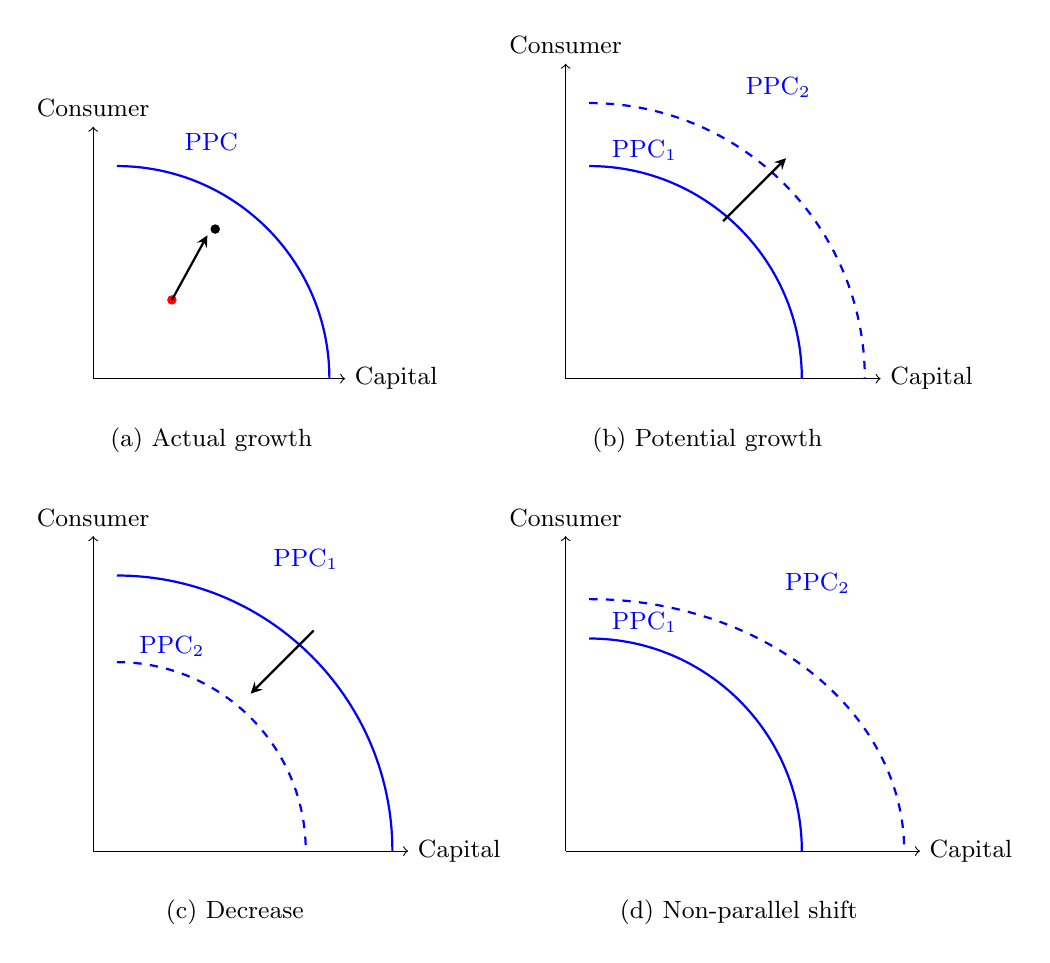
\begin{tikzpicture}
% (a) Actual growth: movement from inside to the curve
\begin{scope}[xshift=0cm, yshift=0cm]
\draw[->] (0,0) -- (3.2,0) node[right, font=\small] {Capital};
\draw[->] (0,0) -- (0,3.2) node[above, font=\small] {Consumer};
\draw[thick, blue] (0.3,2.7) arc (90:0:2.7 and 2.7);
\node[blue, font=\small] at (1.5,3.0) {PPC};
\filldraw[red] (1.0,1.0) circle (1.5pt);
\filldraw (1.55,1.9) circle (1.5pt);
\draw[->, >=stealth, thick] (1.0,1.0) -- (1.45,1.82);
\node[font=\small, below] at (1.5,-0.5) {(a) Actual growth};
\end{scope}
% (b) Growth in production possibilities: outward shift
\begin{scope}[xshift=6cm, yshift=0cm]
\draw[->] (0,0) -- (4.0,0) node[right, font=\small] {Capital};
\draw[->] (0,0) -- (0,4.0) node[above, font=\small] {Consumer};
\draw[thick, blue] (0.3,2.7) arc (90:0:2.7 and 2.7);
\draw[thick, blue, dashed] (0.3,3.5) arc (90:0:3.5 and 3.5);
\node[blue, font=\small] at (1.0,2.9) {PPC$_1$};
\node[blue, font=\small] at (2.7,3.7) {PPC$_2$};
\draw[->, >=stealth, thick] (2.0,2.0) -- (2.8,2.8);
\node[font=\small, below] at (1.8,-0.5) {(b) Potential growth};
\end{scope}
% (c) Decrease in production possibilities: inward shift
\begin{scope}[xshift=0cm, yshift=-6cm]
\draw[->] (0,0) -- (4.0,0) node[right, font=\small] {Capital};
\draw[->] (0,0) -- (0,4.0) node[above, font=\small] {Consumer};
\draw[thick, blue] (0.3,3.5) arc (90:0:3.5 and 3.5);
\draw[thick, blue, dashed] (0.3,2.4) arc (90:0:2.4 and 2.4);
\node[blue, font=\small] at (2.7,3.7) {PPC$_1$};
\node[blue, font=\small] at (1.0,2.6) {PPC$_2$};
\draw[->, >=stealth, thick] (2.8,2.8) -- (2.0,2.0);
\node[font=\small, below] at (1.8,-0.5) {(c) Decrease};
\end{scope}
% (d) Non-parallel shift
\begin{scope}[xshift=6cm, yshift=-6cm]
\draw[->] (0,0) -- (4.5,0) node[right, font=\small] {Capital};
\draw[->] (0,0) -- (0,4.0) node[above, font=\small] {Consumer};
\draw[thick, blue] (0.3,2.7) arc (90:0:2.7 and 2.7);
\draw[thick, blue, dashed] (0.3,3.2) arc (90:0:4.0 and 3.2);
\node[blue, font=\small] at (1.0,2.9) {PPC$_1$};
\node[blue, font=\small] at (3.2,3.4) {PPC$_2$};
\node[font=\small, below] at (2.2,-0.5) {(d) Non-parallel shift};
\end{scope}
\end{tikzpicture}
\end{center}
\subsubsection*{Circular Flow of Income Model}
This model shows the interaction between households and firms.
\begin{itemize}
  \item The model illustrates a closed economy, meaning it has no links with other countries, and is also a model of an economy with no government and no banks or financial market.
  \item It is assumed that the only decision-makers are households and firms.
\end{itemize}
Flow in clockwise direction:
\begin{enumerate}
  \item Households are owners of the FoPs.
  \item Firms buy the FoPs in resource markets and use them to produce G\&S.
  \item They then sell the G\&S to consumers in product markets.
\end{enumerate}
In the counterclockwise direction, there is a flow of money used as payment in sales and purchases.
\begin{enumerate}
  \item When households sell their FoPs, they receive payments taking the form of rent, wages, interest, profit, and are all incomes of households.
  \item Households expenditures are money used to buy G\&S produced by firms.
  \item The payments that firms make to buy FoPs represent their CoP.
  \item The revenue is the payment received by selling G\&S.
\end{enumerate}
\begin{center}
  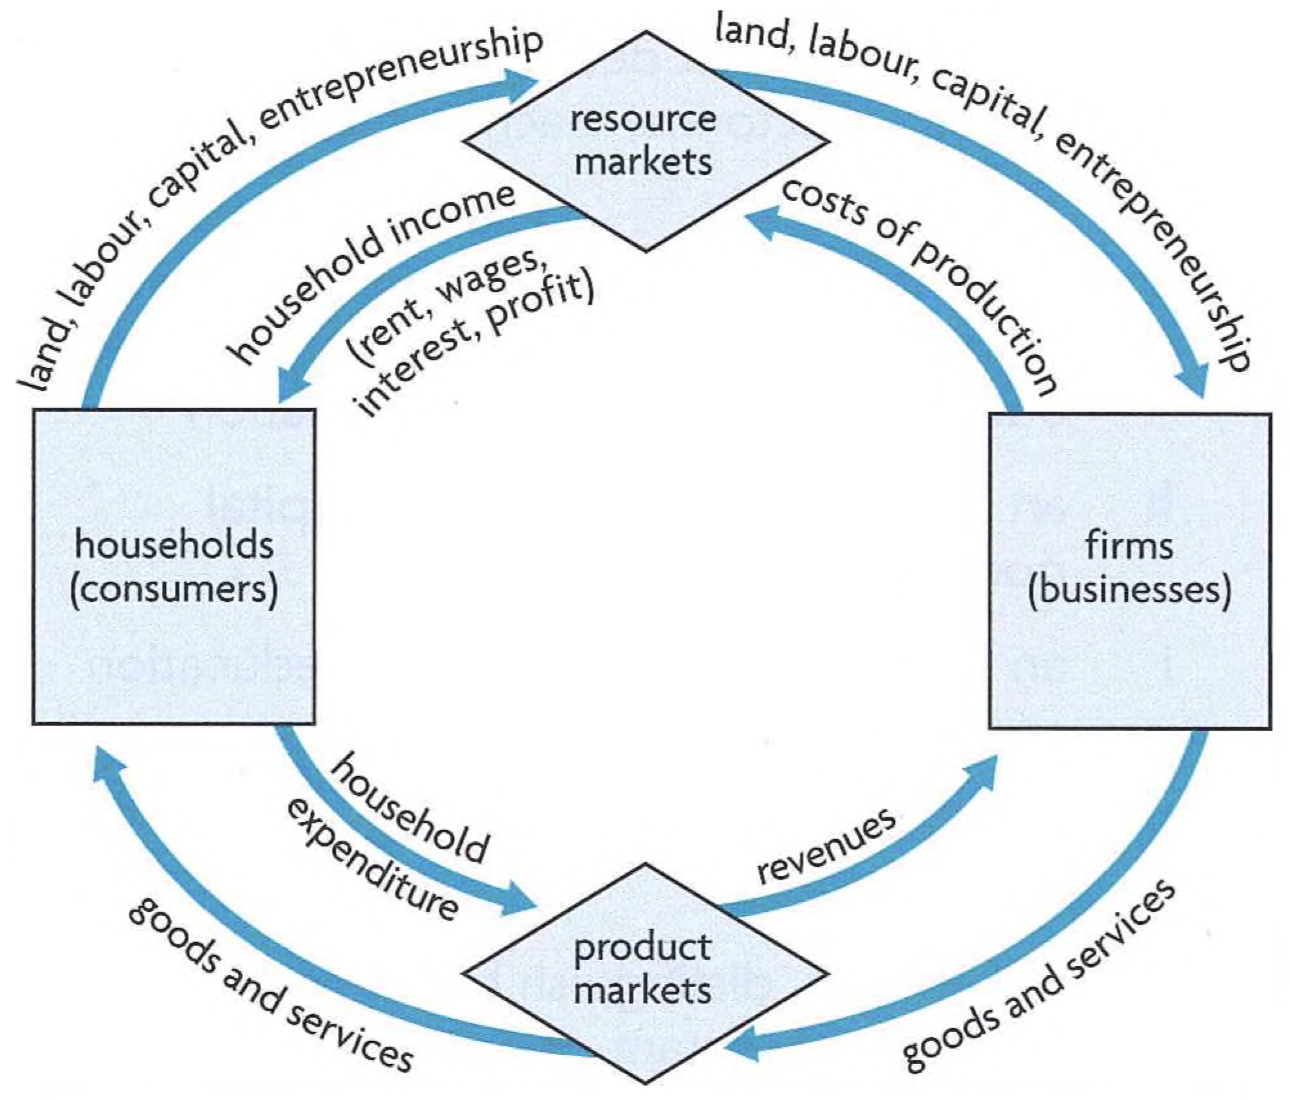
\includegraphics[width=0.55\linewidth]{Screenshot 2026-07-14 at 10.28.33.png}
\end{center}
The circular flow of income shows that in any given time period (say a year), the value of output produced in an economy is equal to the total income generated in producing that output, which is equal to the expenditures made to purchase that output.
\subsubsection*{Injections and leakages}
\textbf{Injection}: additional money added into the circular flow of income.\\
\textbf{Leakage}: money that is taken out of / withdrawn from the circular flow of income.\\
\textbf{Leakages} and \textbf{injections} are paired together so that what leaks out of the flow can come back in as an injection. Some examples include:
\begin{itemize}
  \item Saving \& Investment
  \begin{itemize}
    \item the part of consumer income that is not spent but rather is saved
    \item spending by firms for the production of capital goods
  \end{itemize}
  \item Taxes \& Government spending
  \item Imports \& Exports
  \begin{itemize}
    \item G\&S produced in other countries and purchased by domestic buyers.
    \item G\&S produced domestically and purchased by foreigners.
  \end{itemize}
\end{itemize}
\begin{center}
  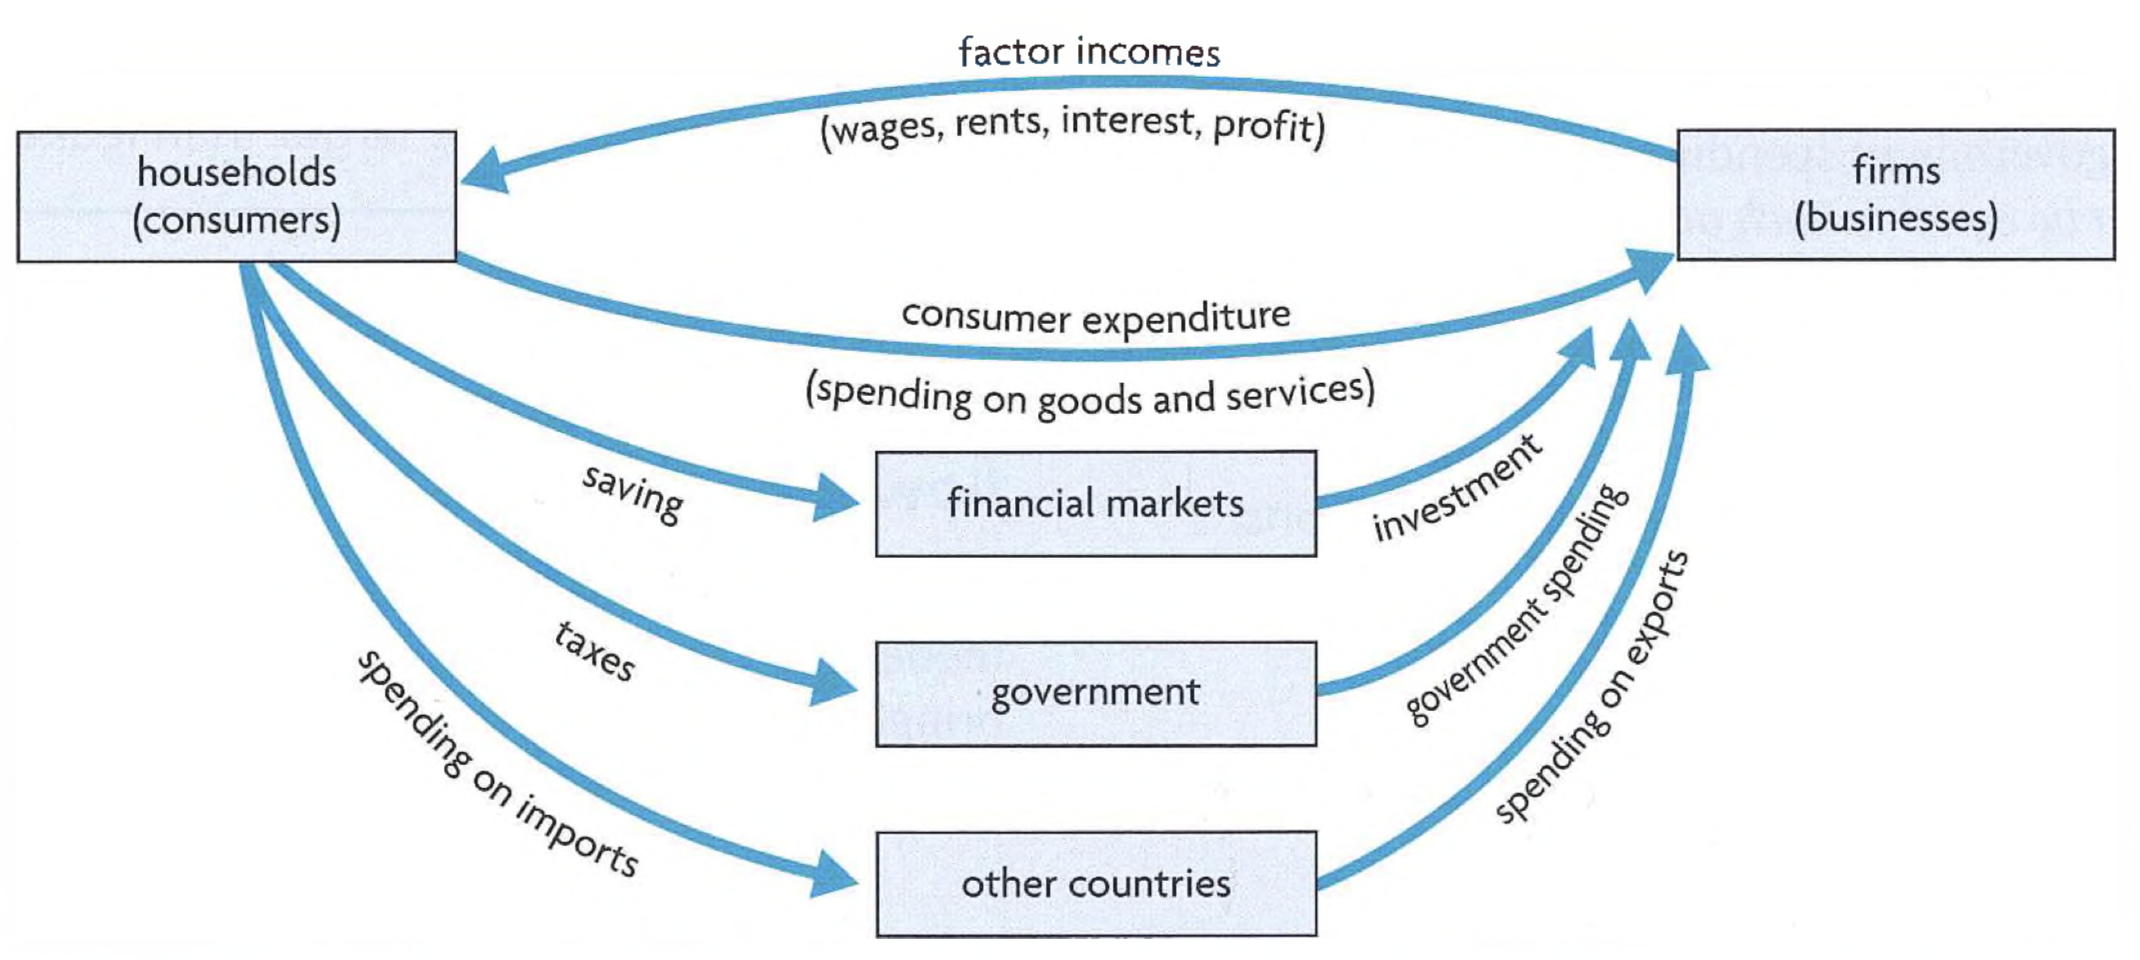
\includegraphics[width=0.75\linewidth]{Screenshot 2026-07-14 at 10.42.23.png}
\end{center}
In the circular flow of income model if injections are larger than leakages the size of the flow increases; if leakages are larger than injections the size of the flow shrinks. (The flow changes for the increase / decrease of domestic reserve of money, which is the total amount of money in the economy.)
\subsection{The method of economics}
\begin{itemize}
  \item \textbf{Positive economics}: study of economics based on the \textbf{scientific method}, to describe, explain and predict economic events. Based on \textbf{positive statements} (about what \textit{is}, \textit{was} or \textit{will be}) that can be tested and shown to be \textbf{true or false}. Uses logic, reasoning, hypotheses, models and theories. Incorporates empirical evidence.
  \item \textbf{Normative economics}: forms the basis of judgements about what economic goals and policies \textit{ought} to be. Based on \textbf{value judgements} (what is good/bad, right/wrong). Can only be \textbf{agreed or disagreed} with, not proven true/false. (看到 \textit{should} $\to$ normative)
\end{itemize}
\subsubsection*{The scientific method in positive economics}
Economists study cause-and-effect relationships between \textbf{variables}:
\begin{enumerate}
  \item \textbf{Identify variables} (e.g.\ price and quantity demanded). Make observations.
  \item Ask questions regarding the observations. 
  \item Form a \textbf{hypothesis} --- an educated guess about an ``if\dots then\dots'' relationship, involving a prediction.
  \item Make predictions. Apply the \textbf{\textit{\emph{ceteris paribus}} assumption} (Latin: ``other things equal'') --- all other variables are held constant so the cause-effect link can be isolated.
  \item Test the hypothesis against \textbf{empirical evidence} (real-world data).
  \item If data support the prediction $\to$ hypothesis accepted; if data contradict $\to$ hypothesis rejected.
\end{enumerate}
A \textbf{theory} is a general explanation of a set of interrelated events, usually based on several successfully tested hypotheses. A \textbf{law} is a well-established, widely accepted generalisation.\\
\textbf{Refutation (falsifiability)}: a hypothesis or theory must be \textit{testable} and capable of being \textbf{disproven}. No matter how many times a hypothesis is tested and accepted, it can never be proven definitively ``true'' --- only ``not yet refuted.'' This ensures economic knowledge is \textit{tentative} and open to revision.
\subsubsection*{The role of normative economics}
\begin{itemize}
  \item \textbf{Value judgements}: subjective beliefs about what is good/bad or right/wrong; underlie all normative statements and policy recommendations.
  \item \textbf{Equity vs equality}: \textbf{equity} = fairness (normative); \textbf{equality} = sameness (positive). Income equality may or may not be equitable depending on the equity principle used (e.g.\ equal distribution vs distribution proportional to work effort). In practice, ``more equitable'' usually means ``more equal'' --- i.e.\ reducing unfair inequalities in income, wealth and opportunity, typically through government intervention.
\end{itemize}
\subsection{A brief history of economic thought, with assist from AI}
\subsubsection*{The 18th century: Adam Smith and \textit{laissez-faire}}
\begin{itemize}
  \item Living at a time when authoritarian government control was increasingly questioned, Smith set out to show that an economy could not only function but thrive \textbf{without} strong government repression.
  \item \textbf{Self-interest + competition}: if each individual pursues self-interest, competition among them regulates behaviour and produces a greater good for society. Competition keeps prices low and directs production toward the goods most wanted.
  \item \textbf{The invisible hand of markets}: thousands of individual decisions, self-regulated through market interactions without government, result in a more efficient use of resources. This is also called a \textbf{\textit{laissez-faire}} economy (French for ``let it do'').
  \item \textbf{Role of government}: limited to three functions --- national defence, justice/security, and public infrastructure (roads, bridges, canals) financed by taxation.
  \item Smith feared monopolies and large corporations that would restrict competition and keep prices high. He believed competition would prevent monopolies from arising.
  \item \textbf{Theory of growth}: growth depends on the \textbf{division of labour} and \textbf{specialisation}, leading to greater output. Extended internationally, this gave rise to the idea of \textbf{absolute advantage} and advocacy of \textbf{free trade}.
  \item In \textit{The Theory of Moral Sentiments} (1759), Smith argued people can \textbf{empathise}; later critics who claimed he justified pure selfishness/greed misread him.
\end{itemize}
\subsubsection*{Supplementary: Specialisation and the division of labour (Edexcel Book 1 Ch 4)}
\needbold{Specialisation}: concentrating production on a limited range of tasks/goods. \needbold{Division of labour}: breaking production into separate tasks done by different workers. Benefits: higher productivity, skill development, time saving, use of machinery. Drawbacks: worker boredom/monotony, over-dependence on specialists, structural unemployment when skills become obsolete.

\subsubsection*{The 19th century --- classical economics}
\textbf{Utility theory in classical microeconomics --- Bentham \& Mill}
\begin{itemize}
  \item \textbf{Jeremy Bentham (1748--1832)} founded \textbf{utilitarianism}: an action is right if it promotes the greatest happiness of the greatest number.
  \item \textbf{John Stuart Mill (1806--1873)} extended Bentham's ideas by blending them with human rights (including minorities and women) and a belief in human freedom.
  \item Both defined \textbf{utility} as that property of an object whereby it produces benefit, pleasure, good or happiness (or prevents mischief, pain, evil). Utility, central to utilitarian ethics, evolved into a central concept of modern economics.
\end{itemize}
\textbf{The concept of the margin}
\begin{itemize}
  \item The \textbf{labour theory of value} (price determined by quantity of labour needed to produce a good) was popular until marginal analysis appeared.
  \item Three economists working independently --- \textbf{Stanley Jevons}, \textbf{Carl Menger} and \textbf{Leon Walras} --- arrived at a theory of prices based on two key ideas: (i) \textbf{utility} (satisfaction from consuming something) is central to value, and (ii) what matters is not total utility but the \textbf{extra/additional utility} of consuming one more unit, i.e.\ \textbf{marginal utility}.
  \item As more units are consumed, marginal utility keeps falling (e.g.\ each successive ice cream gives less satisfaction).
  \item \textbf{Alfred Marshall (1842--1924)}, in the early 20th century, used these ideas to derive the \textbf{law of demand} and the downward-sloping demand curve. The entire demand--supply--equilibrium framework studied today is attributable to Marshall.
\end{itemize}
\textbf{Say's Law in classical macroeconomics}
\begin{itemize}
  \item Named after \textbf{Jean-Baptiste Say (1767--1832)}, the law states simply that \textbf{supply creates its own demand}: overall spending cannot fall enough to prevent all output from being bought.
  \item In the circular flow, firms produce output, pay households income, and households spend that income buying the output; therefore the economy tends toward \textbf{full employment} without govt. intervention.
  \item This idea was seriously questioned during the Great Depression of the 1930s, which saw prolonged falling output and high unemployment --- leading to the birth of macroeconomics as a distinct branch.
\end{itemize}
\textbf{The Marxist critique of classical economics}
\begin{itemize}
  \item \textbf{Karl Marx (1818--1883)} presented a ``scientific'' account of the laws of capitalist development that would eventually result in capitalism's downfall.
  \item Using the labour theory of value, Marx observed that the price of a good usually far exceeded the value of labour (wages) used to produce it. The difference he called \textbf{surplus value}, corresponding to the capitalist's profit --- representing \textbf{exploitation} of workers.
  \item Marx predicted that competition would force capitalists to invest in machinery to cut labour costs; this would reduce surplus value and hence profits, while workers became unemployed and impoverished. The system would be overthrown and replaced by \textbf{communism} (collective ownership of the means of production).
  \item His predictions have \textbf{not} materialised --- capitalist profits have not fallen, and the 20th-century communist regimes arose by force rather than from capitalism's collapse.
  \item Yet Marx remains influential for his insights into capitalism: the recurrence of crises (the business cycle), the impoverishment of the middle class, stagnant real wages, rising income inequality, and job insecurity from technological change.
\end{itemize}
\subsubsection*{The 20th century}
\textbf{The Keynesian revolution}
\begin{itemize}
  \item \textbf{John Maynard Keynes (1883--1946)}, in \textit{The General Theory} (1936), overthrew Say's Law and classical economics by arguing that full employment is only a special case, not a guarantee.
  \item Classical economists thought falls in spending would lower prices and wages, automatically restoring full employment. Keynes countered that wages and prices are \textbf{sticky} (they cannot fall easily); falling wages also reduce workers' spending, further depressing demand.
  \item Therefore the economy cannot self-correct to full employment and requires \textbf{government intervention} --- increased government spending (roads, schools, etc.) that, via the \textbf{multiplier}, produces a multiplied increase in spending and helps the economy escape recession.
  \item Keynes dismissed \textit{laissez-faire} and justified government intervention to avoid prolonged recessions and high unemployment.
\end{itemize}
\textbf{The emergence of macroeconomic policy}
\begin{itemize}
  \item Macroeconomics as a field distinct from microeconomics did not exist until the term was coined by \textbf{Jacob Marschak} in 1945.
  \item Under classical thinking, no macroeconomic policy was needed because the economy was assumed to self-correct. Keynesian ideas inspired active \textbf{demand-side} macroeconomic policy.
\end{itemize}
\textbf{The monetarist/new classical counter-revolution}
\begin{itemize}
  \item In the early 1970s, the oil price crisis caused \textbf{stagflation} (cost-push inflation with stagnant output). Keynesian demand-side theory could not solve this type of inflation.
  \item Two schools gained popularity: \textbf{monetarism} (Milton Friedman, 1912--2006) emphasises the role of money --- changes in money supply affect output in the short run and the price level in the long run; and \textbf{new classical economics} (Robert Lucas, b.\ 1937) emphasises individuals' \textbf{rational expectations} of inflation and policy.
  \item Both share a unifying principle: \textbf{free markets on their own bring the economy back to full employment without government intervention}. Government intervention (minimum wage laws, trade unions, etc.) causes sticky wages/prices that block this automatic adjustment.
  \item This amounts to a \textbf{rejection of Keynesianism} and a return to the classical idea of automatic full employment under \textit{laissez-faire}; hence the term ``new classical.'' It inspired market-based SSP.
\end{itemize}
\subsubsection*{The 21st century}
\textbf{Behavioural economics and the dialogue with psychology}
\begin{itemize}
  \item A growing dialogue between economists and psychologists has produced \textbf{behavioural economics}, which questions the assumption that consumers are rational utility-maximisers.
  \item Consumers often lack the necessary information, and the human mind works in ways that are \textbf{not rational} as standard theory assumes.
  \item Rather than relying on a theory of consumer behaviour, behavioural economics relies on \textbf{experiments and evidence} about how consumers actually behave under varied circumstances, then uses this to design policies that steer consumers toward socially desirable outcomes.
\end{itemize}
\textbf{Interdependence of economy, society and environment; the circular economy}
\begin{itemize}
  \item Until recently economists worked in isolation from environmental and social concerns. There is now growing awareness of the need to consider the \textbf{three pillars of sustainability} together: \textbf{economy, society, environment} (``profit, people, planet'').
  \item The traditional \textbf{linear ``take--make--dispose''} model (extract resources, make products, throw them away) must be replaced by a \textbf{circular economy}: goods should be designed to be repaired rather than discarded, made of biological materials that return safely to the biosphere, keeping resources in use as long as possible and recovering/regenerating products and materials at the end of their life.
\end{itemize}
\newpage
% ------------------------------------------------------------

\section*{Unit 2 Microeconomics}

\section{Competitive markets: Demand and supply}
\subsection{Introduction to competitive markets}
Markets: buyers and sellers of goods, services or resources are linked together to carry out an exchange.\\
Goods and services are sold in product markets, while resources are sold in resource / factor markets.\\\\
Competition: process in which rivals compete in order to achieve some objective.\\
Competitive market: composed of large numbers of sellers and buyers acting independently, so that no one individual seller or small group of sellers has the ability to control the price of the product sold. (market / monopoly power) (through forces of demand and supply instead) Everyone is a price taker.\\\\
A market is any arrangement where those who are willing to and able to buy a good, service, or resource meet those who are willing and able to sell it, and a price is agreed.
\subsection{Demand}
Demand is concerned with the behaviour of buyers. (consumers generally, but can be applied to firms in resource market as well)\\
The demand of an individual consumer indicates the various quantities of a G\&S the consumer is willing (wants to buy the good) and able (can afford to buy it) to buy at different possible prices during a particular time period, \emph{ceteris paribus}.
\begin{center}
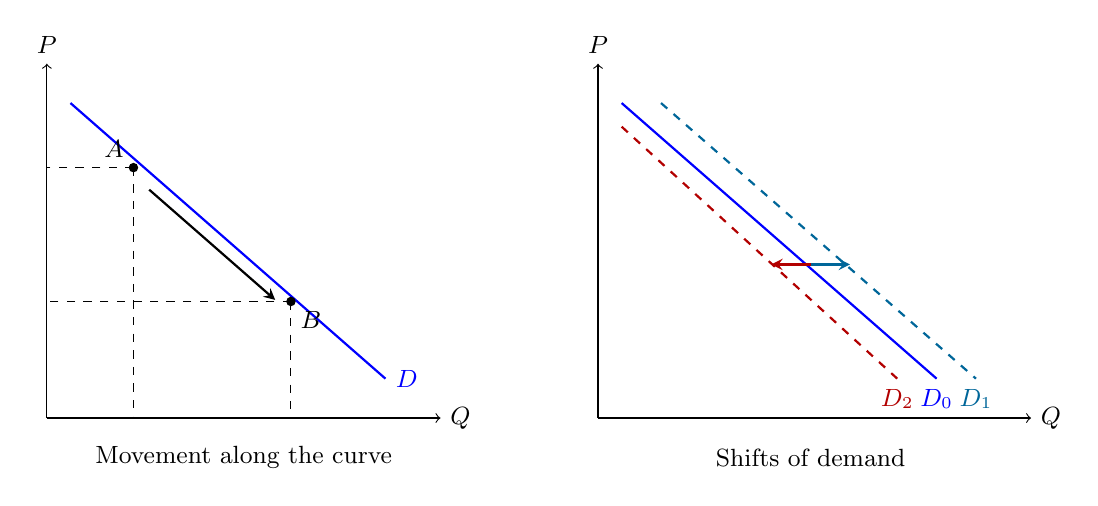
\begin{tikzpicture}
% --- Left panel: movement along the curve ---
\begin{scope}
\draw[->] (0,0) -- (5,0) node[right, font=\small] {$Q$};
\draw[->] (0,0) -- (0,4.5) node[above, font=\small] {$P$};
% Demand curve D
\draw[thick, blue] (0.3,4) -- (4.3,0.5) node[right, blue, font=\small] {$D$};
% Point A (high price, low Q) and B (low price, high Q)
\filldraw (1.1,3.18) circle (1.5pt) node[above left, font=\small] {$A$};
\filldraw (3.1,1.48) circle (1.5pt) node[below right, font=\small] {$B$};
% Dashed guides
\draw[dashed] (1.1,3.18) -- (1.1,0);
\draw[dashed] (1.1,3.18) -- (0,3.18);
\draw[dashed] (3.1,1.48) -- (3.1,0);
\draw[dashed] (3.1,1.48) -- (0,1.48);
% Arrow A->B
\draw[->, >=stealth, thick] (1.3,2.9) -- (2.9,1.5);
\node[font=\small] at (2.5,-0.5) {Movement along the curve};
\end{scope}
% --- Right panel: shifts of the curve ---
\begin{scope}[xshift=7cm]
\draw[->] (0,0) -- (5.5,0) node[right, font=\small] {$Q$};
\draw[->] (0,0) -- (0,4.5) node[above, font=\small] {$P$};
% D0
\draw[thick, blue] (0.3,4) -- (4.3,0.5) node[below, blue, font=\small] {$D_0$};
% D1 (increase -> right shift)
\draw[thick, blue!60!green, dashed] (0.8,4) -- (4.8,0.5) node[below, blue!60!green, font=\small] {$D_1$};
% D2 (decrease -> left shift)
\draw[thick, red!70!black, dashed] (0.3,3.7) -- (3.8,0.5) node[below, red!70!black, font=\small] {$D_2$};
% Shift arrows
\draw[->, >=stealth, thick, blue!60!green] (2.7,1.95) -- (3.2,1.95);
\draw[->, >=stealth, thick, red!70!black] (2.7,1.95) -- (2.2,1.95);
\node[font=\small] at (2.7,-0.5) {Shifts of demand};
\end{scope}
\end{tikzpicture}
\end{center}
\needbold{Market demand} is the sum of all individual demands for a good. The market demand curve illustrates the law of demand, shown by the negative relationship between price and quantity demanded.
\subsubsection*{The law of demand}
There is a negative relationship between the price of a good and its quantity demanded over a particular time period, \emph{ceteris paribus}: as the price of the good increases, quantity demanded falls; as the price falls, quantity demanded increases, \emph{ceteris paribus}. This is reflected as the negative slope of the demand curve. The higher the price of a good, the less of it you are probably willing and able to buy. 
\subsubsection*{Non-price determinants of demand}
\begin{itemize}
  \item Income in the case of normal goods (demand for the good varies directly with income)
  \begin{itemize}
    \item An increase in income leads to a rightward shift in the demand curve.
    \item A decrease in income leads to a leftward shift.
  \end{itemize}
  \item Income in the case of inferior goods (demand for the good varies inversely with income)
  \begin{itemize}
    \item As income increases, consumers switch to more expensive alternatives, demand falls, leftward shift.
    \item As income decreases, occurs in rightward shift.
  \end{itemize}
  \item Preferences and tastes
  \begin{itemize}
    \item If ... change IN favor of the product, demand increases and the demand curve shifts to the right.
    \item If tastes change against the product, demand decreases and the demand curve shifts to the left.
  \end{itemize}
  \item Prices of substitute goods (satisfy similar needs)
  \begin{itemize}
    \item A fall in the price of one results in a fall in the demand for the other.
    \item An increase in the price of one results in an increase in the demand for the other. (switching products)
  \end{itemize}
  \item Prices of complementary goods (tend to be used together)
  \begin{itemize}
    \item A fall in the price of one leads to an increase in the demand for the other.
    \item An increase in the price of one leads to a fall in the demand for the other.
  \end{itemize}
  \item The number of consumers
  \begin{itemize}
    \item If there is an increase in the number of consumers, demand increases and therefore the market demand curve shifts to the right.
    \item If the number of consumers decreases, demand decreases and the curve shifts to the left.
  \end{itemize}
  \item Future expectation of the price
	\begin{itemize}
\item If consumers expect the price of a good to rise in the future, some may purchase the good at the current time period at a comparatively lower price $\rightarrow$ increase in current demand.
\item Vice versa: if consumers expect the price of a product to fall in the future, they may delay their purchase of the good $\rightarrow$ decrease in current demand.
\end{itemize}
\end{itemize}
Any change in price produces a change in quantity demanded, shown as a movement on the demand curve. Any change in a non-price determinant
of demand leads to a change in demand, represented by a shift of the entire demand curve.
\subsubsection*{Assumptions underlying the law of demand: the law of diminishing marginal utility}
\needbold{Utility} is the satisfaction that consumers gain from consuming something. \\
\needbold{Total utility} is the total satisfaction that consumers get from consuming something, while \needbold{marginal utility} is the extra satisfaction that consumers receive from consuming one more unit of a good.
\begin{center}
\begin{tabular}{c|c|c}
\toprule
\textbf{Quantity consumed} & \textbf{Total utility (utils)} & \textbf{Marginal utility (utils)} \\
\midrule
0 & 0 & --- \\
1 & 10 & 10 \\
2 & 18 & 8 \\
3 & 24 & 6 \\
4 & 28 & 4 \\
5 & 30 & 2 \\
6 & 30 & 0 \\
7 & 28 & $-2$ \\
\bottomrule
\end{tabular}
\end{center}
According to the \needbold{law of diminishing marginal utility}, as consumption of a good increases, marginal utility, or the extra utility the consumer receives, decreases with each additional unit consumed. This underlies the law of demand, as it shows that a consumer will be willing to buy an additional unit of a good only if its price falls.
\subsubsection*{Income and substitution effect}
\begin{itemize}
  \item \needbold{The substitution effect}
  \begin{itemize}
    \item If the price of a good falls, the consumer substitutes (buys more) of the now less expensive good. Therefore quantity demanded increases. 
  \end{itemize}
  \item \needbold{The income effect}
  \begin{itemize}
    \item If the real income (purchasing power) increases and price falls, quantity demanded of the good increases.
  \end{itemize}
\end{itemize}
In the case of most goods, whose price is a small fraction of income, the substitution effect is the most important part of the explanation of the law of demand, because being a small fraction of income, the effect that a price change has on real income will be tiny. The income effect becomes important only in the case of purchases of goods whose price take up a large fraction of income.
The above analysis refers to \textbf{normal goods}. In the case of \textbf{inferior goods}, as price falls and real income increases, consumers switch to better alternatives, so the \textbf{income effect is negative} (works \textit{against} the substitution effect). For most inferior goods, the substitution effect still \textit{dominates} the income effect, so the demand curve remains downward sloping.\\
Very rarely, the negative income effect may \textbf{exceed} the substitution effect, so that a fall in price leads to a \textit{decrease} in quantity demanded. This produces an \textbf{upward-sloping demand curve}, and the good is called a \textbf{Giffen good} --- extremely rare in practice.
\begin{center}
\begin{tikzpicture}
\draw[->] (0,0) -- (5,0) node[right, font=\small] {$Q$};
\draw[->] (0,0) -- (0,4.5) node[above, font=\small] {$P$};
\draw[thick, red!70!black] (0.5,0.8) -- (4.0,3.8) node[above left, red!70!black, font=\small] {$D$ (Giffen good)};
\end{tikzpicture}
\end{center}
\subsection{Supply}
Supply is concerned with the behaviour of sellers, which include firms in the product markets and households in resource markets. \\
The supply of an individual firm indicates the various quantities of a G\&S a firm is willing and able to produce and supply to the market for sale at different possible prices, during a particular time period, \emph{ceteris paribus}.\\
Market supply indicates the total quantities of a good that firms are willing and able to supply in the market at different possible prices and is given by the sum of all individual supplies of that good.\\
As with demand, the firm's supply can be presented as a \needbold{supply schedule} (a table listing quantity supplied at various prices), which is then plotted as the \needbold{supply curve}. Market supply is the horizontal sum of all individual firms' supply schedules.
\begin{center}
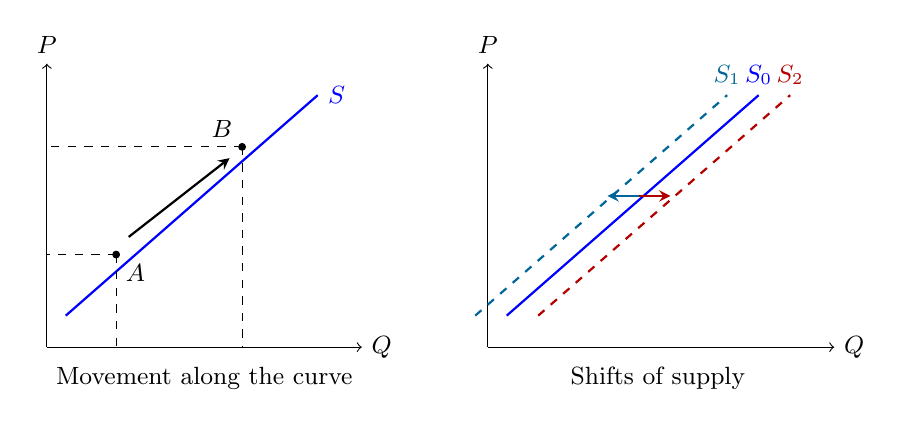
\begin{tikzpicture}[scale=0.8]
% --- Left panel: movement along the curve ---
\begin{scope}
\draw[->] (0,0) -- (5,0) node[right, font=\small] {$Q$};
\draw[->] (0,0) -- (0,4.5) node[above, font=\small] {$P$};
% Supply curve S (upward sloping)
\draw[thick, blue] (0.3,0.5) -- (4.3,4) node[right, blue, font=\small] {$S$};
% Point A (low price, low Q) and B (high price, high Q)
\filldraw (1.1,1.47) circle (1.5pt) node[below right, font=\small] {$A$};
\filldraw (3.1,3.18) circle (1.5pt) node[above left, font=\small] {$B$};
% Dashed guides
\draw[dashed] (1.1,1.47) -- (1.1,0);
\draw[dashed] (1.1,1.47) -- (0,1.47);
\draw[dashed] (3.1,3.18) -- (3.1,0);
\draw[dashed] (3.1,3.18) -- (0,3.18);
% Arrow A->B
\draw[->, >=stealth, thick] (1.3,1.75) -- (2.9,3.0);
\node[font=\small] at (2.5,-0.5) {Movement along the curve};
\end{scope}
% --- Right panel: shifts of the curve ---
\begin{scope}[xshift=7cm]
\draw[->] (0,0) -- (5.5,0) node[right, font=\small] {$Q$};
\draw[->] (0,0) -- (0,4.5) node[above, font=\small] {$P$};
% S0
\draw[thick, blue] (0.3,0.5) -- (4.3,4) node[above, blue, font=\small] {$S_0$};
% S1 (increase -> right shift)
\draw[thick, blue!60!green, dashed] (-0.2,0.5) -- (3.8,4) node[above, blue!60!green, font=\small] {$S_1$};
% S2 (decrease -> left shift)
\draw[thick, red!70!black, dashed] (0.8,0.5) -- (4.8,4) node[above, red!70!black, font=\small] {$S_2$};
% Shift arrows
\draw[->, >=stealth, thick, blue!60!green] (2.4,2.4) -- (1.9,2.4);
\draw[->, >=stealth, thick, red!70!black] (2.4,2.4) -- (2.9,2.4);
\node[font=\small] at (2.7,-0.5) {Shifts of supply};
\end{scope}
\end{tikzpicture}
\end{center}
\subsubsection*{The law of supply}
There is a positive relationship between the quantity of a good supplied over a particular time period and its price, \emph{ceteris paribus}: as the price of the good increases, the quantity of the good supplied also increases; as the price falls, the quantity supplied also falls, \emph{ceteris paribus}. (As price increases, there's more incentive for producers to produce due to increasing profit earned)
\subsubsection*{The vertical supply curve}
A vertical supply curve tells us that even as price increases, the quantity supplied cannot increase; it remains constant. The quantity supplied is independent of price. There are two reasons why this may occur:
\begin{itemize}
  \item There is a fixed quantity of the good supplied because there is no time to produce more of it.
  \item There is a fixed quantity of the good because there is no possibility of ever producing more of it. 
\end{itemize}
\subsubsection*{Non-price determinants of supply curve}
\begin{itemize}
  \item Costs of resources / FoPs
  \item Technological improvements
  \item Price of related goods: Competitive supply
  \begin{itemize}
    \item Competitive supply of two or more products refers to production of one or the other by a firm.
    \item Resources are often limited, therefore producers must choose which type of product should the resource be devoted to.
  \end{itemize}
  \item Prices of related goods: Joint supply
  \begin{itemize}
    \item Joint supply of two or more products refers to production of goods that are derived from a single product, so that it is not possible to produce more of one without producing more of the other.
  \end{itemize}
  \item Producer price expectation
  \begin{itemize}
    \item If firms expect the price of their product to rise, they may withhold some of their current supply from the market, expecting that they will be able to sell it at the higher price in the future.
  \end{itemize}
  \item Taxes (indirect / taxes on profits) (treated as increase in CoP)
  \item Subsidies: a payment made to the firm by the government, = decrease in CoP
  \item Size of the market / the number of firms (increase leads to rightward shift of supply curve)
  \item 'Shocks' or sudden unpredictable events
  \begin{itemize}
    \item e.g. War, weather condition change, catastrophes
  \end{itemize}
\end{itemize}
Any change in price produces a change in quantity supplied, shown as a movement on the supply curve. Any change in a determinant of supply (other than price) produces a change in supply, represented by a shift of the whole supply curve.
\subsubsection*{Assumptions underlying the law of supply: law of diminishing marginal returns}
Difference between short-run SR and long-run LR:
\begin{itemize}
  \item The short run is a time period during which at least one input is fixed and cannot be changed by the firm.
  \item The long run is a time period when all inputs can be changed.
\end{itemize}

\begin{center}
\begin{tabular}{ccc}
\toprule
\textbf{Units of variable input} & \textbf{Total product (TP)} & \textbf{Marginal product (MP)} \\
\midrule
0 & 0 & --- \\
1 & 10 & 10 \\
2 & 22 & 12 \\
3 & 36 & 14 \\
4 & 48 & 12 \\
5 & 58 & 10 \\
6 & 66 & 8 \\
7 & 70 & 4 \\
8 & 70 & 0 \\
9 & 66 & $-4$ \\
\bottomrule
\end{tabular}
\end{center}
According to the law of diminishing marginal returns, as more and more units of a variable input (such as labour) are added to one or more fixed inputs (such as land), the marginal product of the variable input at first increases, but there comes a point when it begins to decrease.
This relationship presupposes that the fixed input(s) remain fixed, and that the technology of production is also fixed.
\subsubsection*{Marginal cost and marginal product}
\needbold{Marginal cost} is the extra or additional cost of producing one more unit of output. It tells us by how much total costs increase if there is an increase in output by one unit.

\begin{center}
\begin{tabular}{ccc}
\toprule
\textbf{Output ($Q$)} & \textbf{Total cost (TC)} & \textbf{Marginal cost (MC)} \\
\midrule
0 & 50 & --- \\
1 & 70 & 20 \\
2 & 85 & 15 \\
3 & 95 & 10 \\
4 & 105 & 10 \\
5 & 120 & 15 \\
6 & 140 & 20 \\
7 & 170 & 30 \\
8 & 210 & 40 \\
\bottomrule
\end{tabular}
\end{center}
When marginal product increases, marginal cost decreases; when marginal product is maximum, marginal cost is minimum; and when marginal product falls, marginal cost increases.
\\\\
$^*:$ It follows then that the firm will be willing and able to supply some quantity as long as the price is enough to cover its costs. Therefore we can think of the supply
curve as showing the price that the firm is willing to accept to produce one more unit of the good. The supply curve begins at the point on the marginal cost curve where the firm is making enough revenue so that it is better off producing than shutting down. (P>AVC)

\begin{center}
\begin{tikzpicture}
% --- Left panel: Marginal product (MP) ---
\begin{scope}
\draw[->] (0,0) -- (5,0) node[right, font=\small] {Units of variable input};
\draw[->] (0,0) -- (0,4.5) node[above, font=\small] {Marginal product};
% MP curve: rises then falls (inverted U)
\draw[thick, blue] (0.3,0.6) .. controls (1.5,3.6) and (3.0,3.6) .. (4.5,0.6)
  node[right, blue, font=\small] {$MP$};
\end{scope}
% --- Right panel: Marginal cost (MC) ---
\begin{scope}[xshift=10cm]
\draw[->] (0,0) -- (5,0) node[right, font=\small] {Output ($Q$)};
\draw[->] (0,0) -- (0,4.5) node[above, font=\small] {Marginal cost};
% MC curve: falls then rises (U-shape)
\draw[thick, red!70!black] (0.3,3.8) .. controls (1.5,0.8) and (3.0,0.8) .. (4.5,3.8)
  node[right, red!70!black, font=\small] {$MC$};
\end{scope}
\end{tikzpicture}
\end{center}
\subsection{Competitive market equilibrium}
Shortages: excess demand. Surplus: excess supply.\\
The existence of excess demand (a shortage)
or excess supply (a surplus) in a free market will cause the price to change so that the quantity demanded will be made equal to quantity supplied. In the event of excess demand, price will rise; in the event of excess supply, price will fall.、、、、
Market equilibrium occurs at a price where quantity demanded = quantity supplied; no surplus / shortage.
\begin{center}
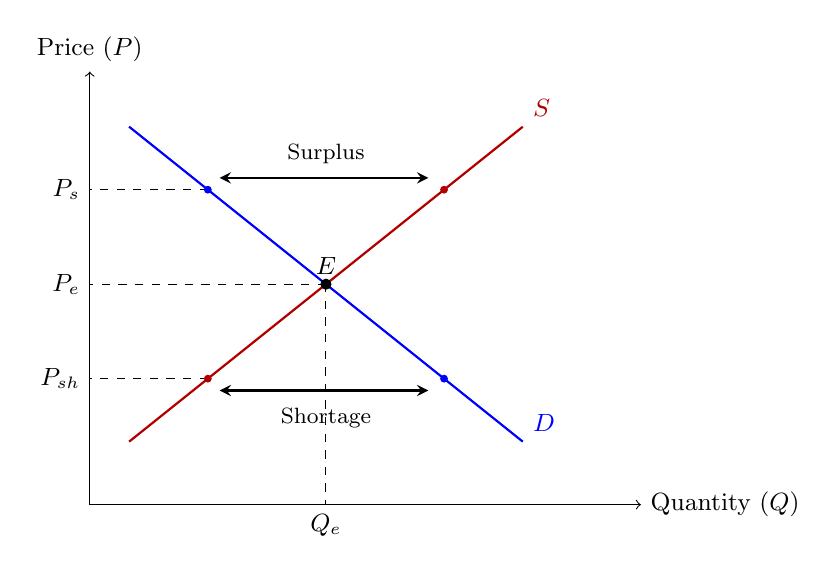
\begin{tikzpicture}
\draw[->] (0,0) -- (7,0) node[right, font=\small] {Quantity ($Q$)};
\draw[->] (0,0) -- (0,5.5) node[above, font=\small] {Price ($P$)};
% Demand curve D
\draw[thick, blue] (0.5,4.8) -- (5.5,0.8) node[above right, blue, font=\small] {$D$};
% Supply curve S
\draw[thick, red!70!black] (0.5,0.8) -- (5.5,4.8) node[above right, red!70!black, font=\small] {$S$};
% Equilibrium point
\filldraw (3.0,2.8) circle (1.8pt) node[above, font=\small] {$E$};
\draw[dashed] (3.0,2.8) -- (3.0,0) node[below, font=\small] {$Q_e$};
\draw[dashed] (3.0,2.8) -- (0,2.8) node[left, font=\small] {$P_e$};
% Surplus: high price P_s
\draw[dashed] (1.5,4.0) -- (0,4.0) node[left, font=\small] {$P_s$};
\filldraw[blue] (1.5,4.0) circle (1.2pt); % Qd at Ps
\filldraw[red!70!black] (4.5,4.0) circle (1.2pt); % Qs at Ps
\draw[<->, >=stealth, thick] (1.65,4.15) -- (4.3,4.15);
\node[font=\footnotesize] at (3,4.45) {Surplus};
% Shortage: low price P_sh
\draw[dashed] (1.5,1.6) -- (0,1.6) node[left, font=\small] {$P_{sh}$};
\filldraw[blue] (4.5,1.6) circle (1.2pt); % Qd at Psh
\filldraw[red!70!black] (1.5,1.6) circle (1.2pt); % Qs at Psh
\draw[<->, >=stealth, thick] (1.65,1.45) -- (4.3,1.45);
\node[font=\footnotesize] at (3,1.1) {Shortage};
\end{tikzpicture}
\end{center}
When quantity demanded is equal to quantity supplied, there is market equilibrium; the
forces of supply and demand are in balance, and there is no tendency for the price to change.
\subsubsection*{Changes in market equilibrium}

\begin{center}
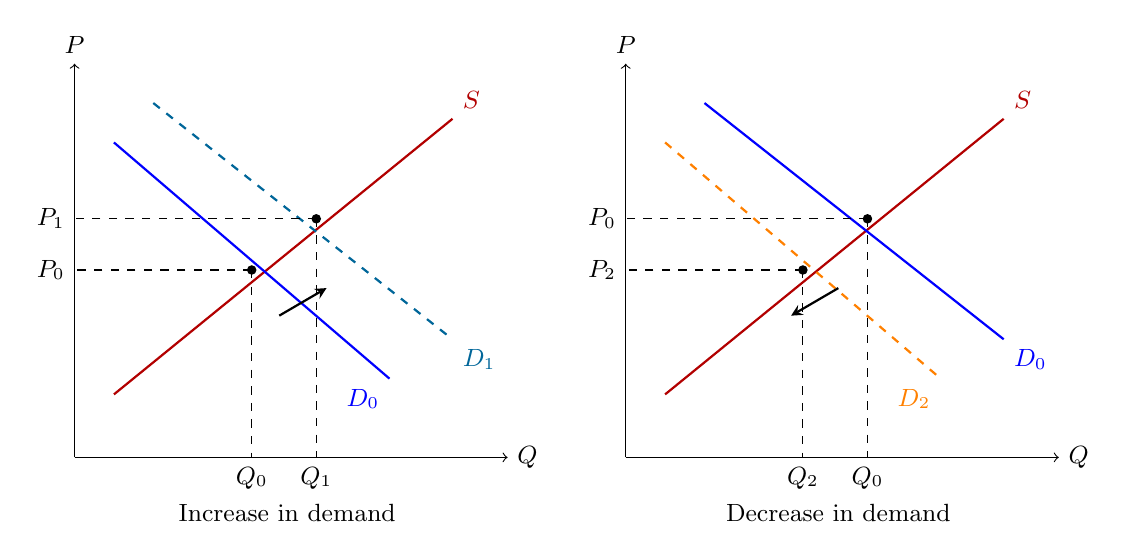
\begin{tikzpicture}
% --- Left panel: increase in demand (rightward shift) ---
\begin{scope}
\draw[->] (0,0) -- (5.5,0) node[right, font=\small] {$Q$};
\draw[->] (0,0) -- (0,5) node[above, font=\small] {$P$};
% Supply
\draw[thick, red!70!black] (0.5,0.8) -- (4.8,4.3) node[above right, red!70!black, font=\small] {$S$};
% D0
\draw[thick, blue] (0.5,4.0) -- (4.0,1.0) node[below left, blue, font=\small] {$D_0$};
% D1 (rightward shift)
\draw[thick, blue!60!green, dashed] (1.0,4.5) -- (4.8,1.5) node[below right, blue!60!green, font=\small] {$D_1$};
% Original equilibrium
\filldraw (2.25,2.38) circle (1.5pt);
\draw[dashed] (2.25,2.38) -- (2.25,0) node[below, font=\small] {$Q_0$};
\draw[dashed] (2.25,2.38) -- (0,2.38) node[left, font=\small] {$P_0$};
% New equilibrium
\filldraw (3.07,3.03) circle (1.5pt);
\draw[dashed] (3.07,3.03) -- (3.07,0) node[below, font=\small] {$Q_1$};
\draw[dashed] (3.07,3.03) -- (0,3.03) node[left, font=\small] {$P_1$};
% Shift arrow
\draw[->, >=stealth, thick] (2.6,1.8) -- (3.2,2.15);
\node[font=\small] at (2.7,-0.7) {Increase in demand};
\end{scope}
% --- Right panel: decrease in demand (leftward shift) ---
\begin{scope}[xshift=7cm]
\draw[->] (0,0) -- (5.5,0) node[right, font=\small] {$Q$};
\draw[->] (0,0) -- (0,5) node[above, font=\small] {$P$};
% Supply
\draw[thick, red!70!black] (0.5,0.8) -- (4.8,4.3) node[above right, red!70!black, font=\small] {$S$};
% D0
\draw[thick, blue] (1.0,4.5) -- (4.8,1.5) node[below right, blue, font=\small] {$D_0$};
% D2 (leftward shift)
\draw[thick, orange, dashed] (0.5,4.0) -- (4.0,1.0) node[below left, orange, font=\small] {$D_2$};
% Original equilibrium
\filldraw (3.07,3.03) circle (1.5pt);
\draw[dashed] (3.07,3.03) -- (3.07,0) node[below, font=\small] {$Q_0$};
\draw[dashed] (3.07,3.03) -- (0,3.03) node[left, font=\small] {$P_0$};
% New equilibrium
\filldraw (2.25,2.38) circle (1.5pt);
\draw[dashed] (2.25,2.38) -- (2.25,0) node[below, font=\small] {$Q_2$};
\draw[dashed] (2.25,2.38) -- (0,2.38) node[left, font=\small] {$P_2$};
% Shift arrow
\draw[->, >=stealth, thick] (2.7,2.15) -- (2.1,1.8);
\node[font=\small] at (2.7,-0.7) {Decrease in demand};
\end{scope}
\end{tikzpicture}

\vspace{0.8cm}

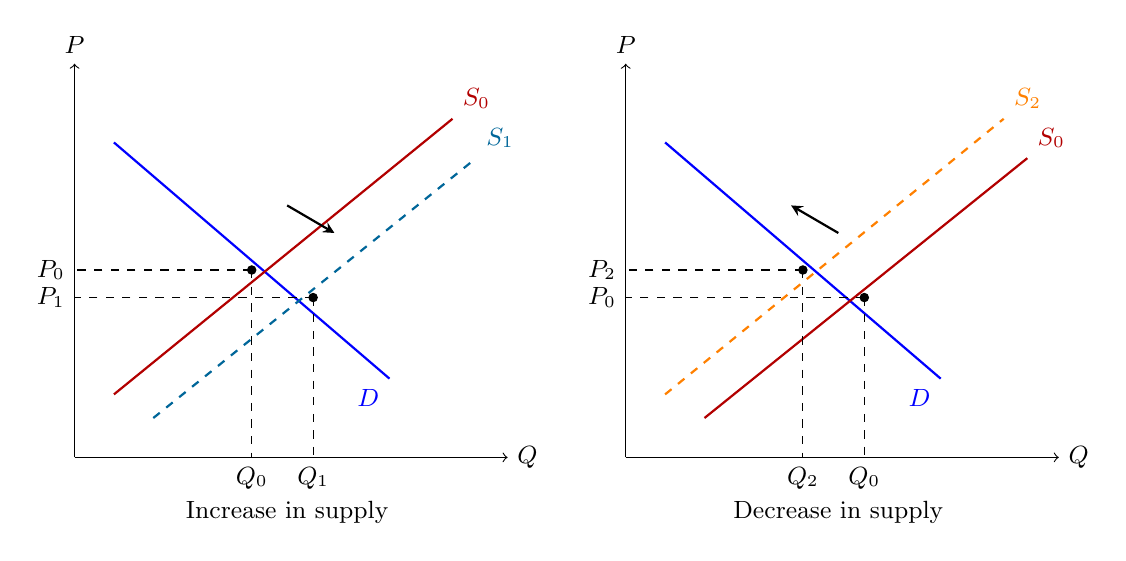
\begin{tikzpicture}
% --- Left panel: increase in supply (rightward shift) ---
\begin{scope}
\draw[->] (0,0) -- (5.5,0) node[right, font=\small] {$Q$};
\draw[->] (0,0) -- (0,5) node[above, font=\small] {$P$};
% Demand
\draw[thick, blue] (0.5,4.0) -- (4.0,1.0) node[below left, blue, font=\small] {$D$};
% S0
\draw[thick, red!70!black] (0.5,0.8) -- (4.8,4.3) node[above right, red!70!black, font=\small] {$S_0$};
% S1 (rightward shift)
\draw[thick, blue!60!green, dashed] (1.0,0.5) -- (5.1,3.8) node[above right, blue!60!green, font=\small] {$S_1$};
% Original equilibrium
\filldraw (2.25,2.38) circle (1.5pt);
\draw[dashed] (2.25,2.38) -- (2.25,0) node[below, font=\small] {$Q_0$};
\draw[dashed] (2.25,2.38) -- (0,2.38) node[left, font=\small] {$P_0$};
% New equilibrium
\filldraw (3.03,2.03) circle (1.5pt);
\draw[dashed] (3.03,2.03) -- (3.03,0) node[below, font=\small] {$Q_1$};
\draw[dashed] (3.03,2.03) -- (0,2.03) node[left, font=\small] {$P_1$};
% Shift arrow
\draw[->, >=stealth, thick] (2.7,3.2) -- (3.3,2.85);
\node[font=\small] at (2.7,-0.7) {Increase in supply};
\end{scope}
% --- Right panel: decrease in supply (leftward shift) ---
\begin{scope}[xshift=7cm]
\draw[->] (0,0) -- (5.5,0) node[right, font=\small] {$Q$};
\draw[->] (0,0) -- (0,5) node[above, font=\small] {$P$};
% Demand
\draw[thick, blue] (0.5,4.0) -- (4.0,1.0) node[below left, blue, font=\small] {$D$};
% S0
\draw[thick, red!70!black] (1.0,0.5) -- (5.1,3.8) node[above right, red!70!black, font=\small] {$S_0$};
% S2 (leftward shift)
\draw[thick, orange, dashed] (0.5,0.8) -- (4.8,4.3) node[above right, orange, font=\small] {$S_2$};
% Original equilibrium
\filldraw (3.03,2.03) circle (1.5pt);
\draw[dashed] (3.03,2.03) -- (3.03,0) node[below, font=\small] {$Q_0$};
\draw[dashed] (3.03,2.03) -- (0,2.03) node[left, font=\small] {$P_0$};
% New equilibrium
\filldraw (2.25,2.38) circle (1.5pt);
\draw[dashed] (2.25,2.38) -- (2.25,0) node[below, font=\small] {$Q_2$};
\draw[dashed] (2.25,2.38) -- (0,2.38) node[left, font=\small] {$P_2$};
% Shift arrow
\draw[->, >=stealth, thick] (2.7,2.85) -- (2.1,3.2);
\node[font=\small] at (2.7,-0.7) {Decrease in supply};
\end{scope}
\end{tikzpicture}
\end{center}
\subsubsection*{Free goods revisited}
A free good is a good for which the quantity supplied is greater than the quantity demanded when the price is zero. Supply
is so large relative to demand that there is excess quantity supplied even at a zero price. A free good can change into an economic good as a result of a leftward shift in the supply curve (reduced supply)
or a rightward shift in the demand curve (increased demand). When demand and supply intersect at a price greater than zero, the good has become an economic good.

\begin{center}
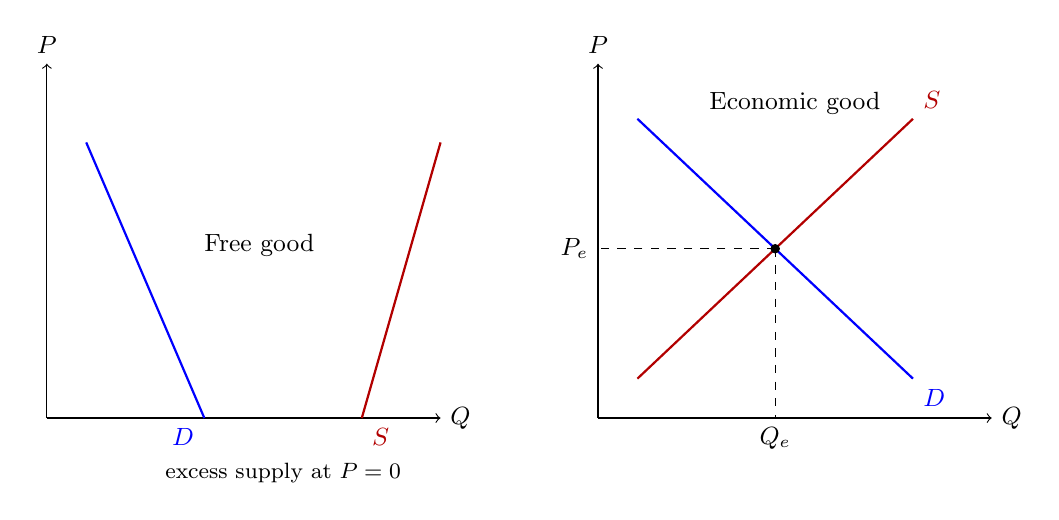
\begin{tikzpicture}
% --- Left: Free good ---
\begin{scope}
\draw[->] (0,0) -- (5,0) node[right, font=\small] {$Q$};
\draw[->] (0,0) -- (0,4.5) node[above, font=\small] {$P$};
% Demand curve (intersects x-axis at low Q)
\draw[thick, blue] (0.5,3.5) -- (2,0) node[below left, blue, font=\small] {$D$};
% Supply curve (far to the right, intersects x-axis at high Q)
\draw[thick, red!70!black] (5,3.5) -- (4,0) node[below right, red!70!black, font=\small] {$S$};
% Excess supply bracket at P=0
\node[font=\footnotesize] at (3,-0.7) {excess supply at $P=0$};
\node[font=\small] at (2.7,2.2) {Free good};
\end{scope}
% --- Right: Economic good ---
\begin{scope}[xshift=7cm]
\draw[->] (0,0) -- (5,0) node[right, font=\small] {$Q$};
\draw[->] (0,0) -- (0,4.5) node[above, font=\small] {$P$};
% Demand
\draw[thick, blue] (0.5,3.8) -- (4.0,0.5) node[below right, blue, font=\small] {$D$};
% Supply
\draw[thick, red!70!black] (0.5,0.5) -- (4.0,3.8) node[above right, red!70!black, font=\small] {$S$};
% Equilibrium
\filldraw (2.25,2.15) circle (1.5pt);
\draw[dashed] (2.25,2.15) -- (2.25,0) node[below, font=\small] {$Q_e$};
\draw[dashed] (2.25,2.15) -- (0,2.15) node[left, font=\small] {$P_e$};
\node[font=\small] at (2.5,4) {Economic good};
\end{scope}
\end{tikzpicture}
\end{center}
\subsection{The role of the price mechanism and market efficiency}
Prices determined by the forces of supply and demand in competitive markets are known as the \needbold{price mechanism}.\\
The invisible hand succeeds in coordinating the buying and selling decisions of thousands or millions of decision-makers in an economy without any central authority. 
\begin{itemize}
  \item The what / how much to produce question of resource allocation is answered because firms produce only those goods consumers are willing and able to buy, while consumers buy only those goods producers are willing and able to supply.
  \item The how to produce question of resource allocation is answered because firms use those resources and technologies in their production process that they are willing and able to pay for.
\end{itemize}
The key to the market's ability to allocate resources can be found in the signalling and incentive functions of prices in resource allocation. 
\begin{itemize}
  \item As signals, prices communicate information to decision-makers (shortage / surplus) for making production and consumption decisions in order to allocate resources.
  \item As incentives, prices motivate decision-makers to respond to the information. (increase / decrease production) This results in a reallocation of resources for maximizing benefits.
\end{itemize}
\needbold{Rationing}: a method of apportioning or parceling out goods and services among consumers or households. The market mechanism uses price rationing for this purpose, which involves the use of prices freely determined in markets. Serves to allocate scarce resources by increasing the market price to deter some consumers from buying the good.
\subsubsection*{Allocative efficiency}
Allocative efficiency refers to producing the quantity of goods mostly wanted by society, achieved when the economy allocates its resources so that the society gets the most benefits from consumption. 
\begin{itemize}
  \item Demand as marginal benefit curve
  \begin{itemize}
    \item Marginal benefit: the extra benefit that you get from each additional unit of something you buy
    \item The demand curve can also be thought of as showing the amount of money that the consumer is willing to pay to get one more unit of the good.
    \item Since marginal benefit decreases as the quantity of a good consumed increases, consumers will be willing to buy an extra unit of the good only if its price falls.
    \item $\therefore D=MB$
    \item (Marginal utility $\neq$ Marginal benefit (indicate the consumer's willingness to pay for the last or marginal unit bought / price))
  \end{itemize}
  \item Supply as marginal cost curve
  \begin{itemize}
    \item Marginal cost: the extra cost of producing one more unit of output
    \item The supply curve also shows the price that the firm is willing to accept in order to produce one more unit of the good.
    \item Since marginal cost increases as the quantity of a good produced increases, producers will be willing to produce and sell an extra unit of the good only of its price increases. 
    \item $\therefore S=MC$
  \end{itemize}
\end{itemize}
In order to achieve allocative efficiency, $MB=MC$. Practically, it means that the extra benefit to society of getting one more unit of the good is equal to the extra cost to society of producing one more unit of the good. When this happens, society's resources are being
used to produce the 'right' quantity of the good.
\begin{itemize}
  \item If $MB>MC$, society would be placing a greater value on the last unit of the good produced than it costs to produce it, and so more of it should be produced.
  \item If $MB<MC$, it would be costing society more to produce the last unit of the good produced than the value society puts on it, and so less should be produced.
\end{itemize}
\subsubsection*{Consumer and producer surplus}
Consumer surplus (for a specific quantity) is defined as the price consumers are willing to pay for a good minus the price actually paid. It is the area under the demand curve and below the price paid by the consumer, up to the quantity purchased.
\[\text{Consumer Surplus}=\dfrac{1}{2}(P_\text{intercept of D}-P_e)\times Q_e\]
Producer surplus (for a specific quantity) is defined as the price received by firms for selling their good minus the price that they are willing to accept to produce the good. It is shown as the area above the firms' supply curve and below the price received by the firm, up to the quantity produced.
\[\text{Producer Surplus}=\dfrac{1}{2}(P_e-P_\text{intercept of S})\times Q_e\left(=\dfrac{1}{2}(Q_\text{intercept of S}+Q_e)\times P_e\right)\]
(Note when supply curve has a Q-intercept, producer can be determined using formula for area of a trapezium)

\begin{center}
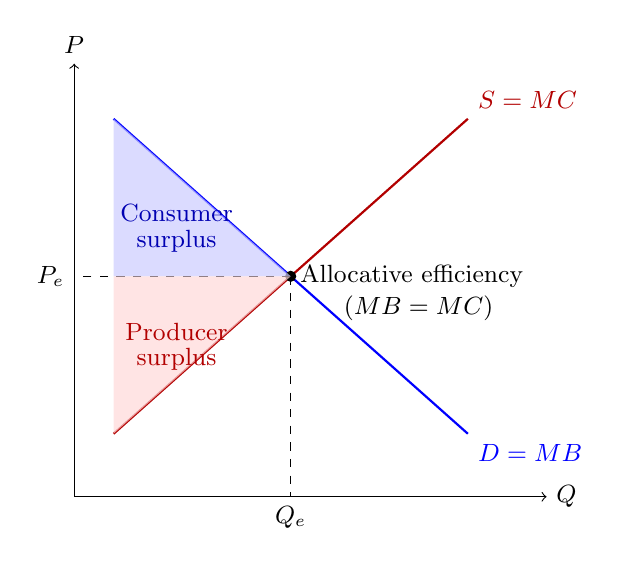
\begin{tikzpicture}
\draw[->] (0,0) -- (6,0) node[right, font=\small] {$Q$};
\draw[->] (0,0) -- (0,5.5) node[above, font=\small] {$P$};
% D = MB
\draw[thick, blue] (0.5,4.8) -- (5.0,0.8) node[below right, blue, font=\small] {$D = MB$};
% S = MC
\draw[thick, red!70!black] (0.5,0.8) -- (5.0,4.8) node[above right, red!70!black, font=\small] {$S = MC$};
% Equilibrium point
\filldraw (2.75,2.8) circle (1.8pt);
\node[right, font=\small] at (2.75,2.8) {Allocative efficiency};
\node[right, font=\small] at (3.3,2.4) {($MB=MC$)};
\draw[dashed] (2.75,2.8) -- (2.75,0) node[below, font=\small] {$Q_e$};
\draw[dashed] (2.75,2.8) -- (0,2.8) node[left, font=\small] {$P_e$};
% Consumer surplus: triangle above P_e, below D, up to Q_e
\fill[blue!20, opacity=0.7] (0.5,4.8) -- (2.75,2.8) -- (0.5,2.8) -- cycle;
\node[blue!70!black, font=\small] at (1.3,3.6) {Consumer};
\node[blue!70!black, font=\small] at (1.3,3.25) {surplus};
% Producer surplus: triangle below P_e, above S, up to Q_e
\fill[red!15, opacity=0.7] (0.5,0.8) -- (2.75,2.8) -- (0.5,2.8) -- cycle;
\node[red!70!black, font=\small] at (1.3,2.1) {Producer};
\node[red!70!black, font=\small] at (1.3,1.75) {surplus};
\end{tikzpicture}
\end{center}
At the point of competitive market equilibrium, the sum of consumer and producer surplus is maximum.\\
At equilibrium, social surplus, defined as the sum of consumer plus producer surplus, is maximum. Therefore maximum social surplus is just another way of saying that there is allocative efficiency.
Social welfare, the amount of consumer and producer surplus, is maximized as well.
\subsubsection*{Allocative efficiency of markets vs Govt. Intervention}
Issues with market allocative efficiency:
\begin{itemize}
  \item Efficiency can only arise under a number of very strict and highly unrealistic conditions that are practically never met in the real world.
  \begin{itemize}
    \item When markets fail to achieve allocative efficiency, this means that social surplus is reduced, resulting in what is known as welfare loss / deadweight loss.
    \item In other words, social welfare is no longer maximum on account of a portion of it being lost.
  \end{itemize}
  \item The competitive market is unable to provide a satisfactory answer to the for whom to produce question.
\end{itemize}
\subsubsection*{Supplementary: Pareto efficiency / Pareto optimality (welfare economics)}
\needbold{Pareto efficiency (Pareto optimality)} is a condition of resource allocation in which \textbf{it is impossible to make any one person better off without making at least one other person worse off}. A \needbold{Pareto improvement} is a reallocation that makes at least one person better off without making anyone worse off; an allocation is Pareto efficient when no Pareto improvement is possible.
\begin{itemize}
  \item \textbf{Link to allocative efficiency}: in the competitive market model, free-market equilibrium produces allocative efficiency ($MB = MC$ or $MSB = MSC$), meaning maximum social surplus --- and it is not possible to make anyone better off without making someone worse off. Thus allocative efficiency at the competitive equilibrium corresponds to \textbf{Pareto optimality}.
  \item \textbf{PPC interpretation}: points \textit{on} the PPC are Pareto efficient in production --- producing more of one good requires producing less of the other (someone must give up something); points \textit{inside} the PPC are Pareto inefficient because output can be increased without making anyone worse off.
  \item \textbf{Equity caveat (important for evaluation)}: Pareto efficiency says \textbf{nothing about the distribution of income}. An allocation can be Pareto optimal while being highly unequal (e.g.\ one person owns almost everything). It also embodies the value judgement that ``welfare'' equals maximum social surplus, ignoring the \textit{for whom} question --- so it should not be treated as a value-free standard for judging outcomes.
\end{itemize}
\subsection{Critique of the maximising behaviour of consumers and producers}
The assumption of \textbf{rational self-interest} --- that consumers maximise utility and firms maximise profit --- has come under serious challenge from \textbf{behavioural economics}.
\subsubsection*{Assumptions of rational consumer choice}
\begin{itemize}
  \item \textbf{Completeness}: the consumer can rank any two bundles (prefers A to B, B to A, or is indifferent).
  \item \textbf{Transitivity}: if A is preferred to B, and B to C, then A is preferred to C (preferences are consistent).
  \item \textbf{Non-satiation}: the consumer always prefers more of a good to less.
  \item \textbf{Perfect information}: consumers know all possible products, qualities and prices.
  \item \textbf{Utility maximisation}: consumers buy the combination of goods that yields the greatest total utility for a given budget.
\end{itemize}
\subsubsection*{Supplementary: Consumer choice theory (AP Barron Ch 5)}
IB discusses rational choice assumptions and behavioural economics, but AP/Edexcel exams add the \textbf{graphical/mathematical model}:
\begin{itemize}
  \item \needbold{Budget constraint (budget line)}: shows all combinations of two goods the consumer can afford, given income $M$ and prices $P_x, P_y$:
  \[P_x x + P_y y = M \qquad \text{slope} = -\dfrac{P_x}{P_y}\]
  A change in income shifts the line in parallel; a change in one price rotates it.
  \item \needbold{Indifference curve}: shows combinations of two goods giving the consumer the \textbf{same total utility}. Properties: downward-sloping; convex to the origin (diminishing marginal rate of substitution); indifference curves do not cross; higher curves represent higher utility.
  \item \needbold{Consumer optimum}: the best affordable bundle is where the budget line is \textbf{tangent} to the highest attainable indifference curve. At that point, the slope of the budget line equals the slope of the indifference curve:
  \[\dfrac{MU_x}{P_x}=\dfrac{MU_y}{P_y}\]
  (the \needbold{utility-maximization rule}: marginal utility per dollar is equalised across all goods).
  \item \textbf{Adjustment logic}: if $\frac{MU_x}{P_x} > \frac{MU_y}{P_y}$, the consumer gains utility by buying more $X$ and less $Y$; buying continues until equality holds.
\end{itemize}
\subsubsection*{Behavioural economics: limitations of rational behaviour}
\textbf{Behavioural economics} (influenced by psychology, sociology, neuroscience) argues human behaviour is far more complex than rationality assumes.\\
\textbf{Cognitive biases} --- systematic errors in thinking:
\begin{itemize}
  \item \textbf{Rules of thumb}: simple mental shortcuts based on experience that simplify complex decisions (e.g.\ estimating a portion size by a handful).
  \item \textbf{Anchoring}: relying on irrelevant initial information when making decisions (e.g.\ a ``was \$150, now \$100'' sign makes \$100 seem cheap even if the good is worth \$50).
  \item \textbf{Framing}: choices are affected by how options are presented (e.g.\ ``80\% lean'' is preferred to ``20\% fat'' despite being identical information).
  \item \textbf{Availability}: over-reliance on the most recently available information rather than all relevant data (e.g.\ choosing a brand due to recent heavy advertising).
\end{itemize}
\textbf{Alternative concepts challenging full rationality:}
\begin{itemize}
  \item \textbf{Bounded rationality} (Herbert Simon, Nobel 1978): consumers are rational only \textit{within limits}, constrained by insufficient information, the cost of acquiring information, and the brain's limited processing capacity. Rather than maximise, consumers \textbf{satisfice} --- they seek a \textit{satisfactory} rather than optimal outcome.
  \item \textbf{Bounded self-control}: people exercise self-control only within limits (e.g.\ eating too much, saving too little) --- inconsistent with rational behaviour.
  \item \textbf{Bounded selfishness}: people are selfish only within limits; altruism, charity and fairness cannot be explained by pure self-interest.
  \item \textbf{Imperfect information}: in reality consumers never have full information, so choices are based on incomplete and faulty data --- utility cannot be maximised.
\end{itemize}
\subsubsection*{Behavioural economics in policy: nudge theory and choice architecture}
\textbf{Nudge theory}: a \textbf{nudge} influences consumers' choices in a predictable way \textit{without} financial incentives, sanctions, or restricting freedom of choice. Many governments have established \textbf{nudge units}.
\\
\textbf{Choice architecture}: the design of the context/environment in which people make choices. Key types:
\begin{itemize}
  \item \textbf{Default choice}: the option that results if one does nothing; people often stick with defaults out of habit or inertia (e.g.\ opt-out organ donation $\to$ far higher donor rates than opt-in).
  \item \textbf{Restricted choice}: choices limited by government or social norms (e.g.\ speed limits, smoking bans) to prevent poor decisions.
  \item \textbf{Mandated choice}: a free choice that is compulsory to make (e.g.\ must declare organ-donor status to renew a driver's licence).
\end{itemize}
\textit{Note:} nudges can backfire if people feel manipulated (e.g.\ the Netherlands' opt-out organ donation law led to a surge in non-donors).
\subsubsection*{Mainstream response and evaluation}
\begin{itemize}
  \item \textbf{In defence of rationality}: despite imperfections, utility theory explains and predicts consumer behaviour well \textit{on average} (e.g.\ downward-sloping demand curves are empirically confirmed).
  \item \textbf{Critique of nudges}: may be \textbf{manipulative}, exploiting incomplete information at a sub-conscious level; choice architecture may be disguised government regulation. There should be \textbf{transparency} about nudges used in policy.
  \item \textbf{Advantages} of behavioural policies: low-cost, freedom-preserving, evidence-based (tested through experiments), flexible.
  \item \textbf{Disadvantages}: no unifying theory of behaviour; results may not generalise across cultures/time; may substitute for more effective traditional policies (taxes, subsidies); risk of manipulation.
\end{itemize}
\subsubsection*{Firm business objectives}
\textbf{Rational producer behaviour}: standard theory assumes firms pursue \textbf{profit maximisation} --- producing the output level that makes $\text{profit} = \text{total revenue} - \text{total cost}$ as large as possible.
\\
\textbf{Alternative business objectives}:
\begin{itemize}
  \item \textbf{Corporate social responsibility}: firms engage in ethical/environmentally responsible behavior (avoiding pollution, shunning child labour, charitable donations) because irresponsible behaviour can reduce revenues via consumer backlash and invite government regulation.
  \item \textbf{Market share}: the percentage of total market sales earned by a firm. A high/growing share indicates strong performance relative to competitors and may allow \textbf{economies of scale}; firms may sacrifice some profit (lower prices, R\&D spending, advertising) to maintain or grow market share.
  \item \textbf{Growth maximisation}: maximising the firm's size rather than profit. Growth brings economies of scale, diversification, greater market power, reduced risk of takeover, and reconciles interests of both owners and managers.
  \item \textbf{Revenue maximisation}: managers (as distinct from owners) may pursue maximum sales revenue, as it is more easily measured and linked to managerial rewards. (Not in syllabus.)
  \item \textbf{Satisficing}: large firms have many conflicting internal groups with multiple objectives; rather than maximising any single variable, firms pursue a \textbf{satisfactory} level of profit alongside satisfactory results on many objectives.
\end{itemize}
\section{Elasticities}
In economics, elasticity refers to the overall responsiveness of a variable as a result of a change in another variable.
\subsection{Price elasticity of demand (PED)}
Price elasticity of demand is a measure of the responsiveness of the quantity of a good demanded to changes in its price. (Note that although the value calculated is going to be negative, the common practice is to drop the minus sign and consider PED as a positive number / take the absolute value)
\begin{itemize}
  \item If quantity demanded is highly responsive to a change in price, $PED>1$ demand is price elastic; change in price leads to a proportionally larger change in $Q_d$
  \item If quantity demanded is not very responsive, $PED<1$ demand is price inelastic; change in price leads to a proportionally smaller change in $Q_d$
  \item Demand is unit elastic when $PED=1$, also called unitary PED.
  \item Demand is perfectly inelastic when $PED=0$.
  \item Demand is perfectly elastic when $PED=\infty$.
\end{itemize}
\[PED=\dfrac{\%\Delta Q_d}{\%\Delta P}=\dfrac{\dfrac{Q_2-Q_1}{Q_1}}{\dfrac{P_2-P_1}{P_1}}\]
Midpoint formula for PED calculation:
\[PED=\dfrac{\dfrac{\Delta Q_d}{Q_\text{avg}}}{\dfrac{\Delta P_d}{P_\text{avg}}}=\dfrac{\dfrac{\Delta Q}{\dfrac{1}{2}(Q_1+Q_2)}}{\dfrac{\Delta P}{\dfrac{1}{2}(P_1+P_2)}}\]
In general, when demand curves intersect, then for any given price, the flatter the demand curve, the more elastic is the demand. The steeper the demand curve, the less elastic the demand.
\subsubsection*{Changing PED and the straight-line demand curve}
Along any downward-sloping, straight-line demand curve, the PED varies (changes) as we move along the curve.

\begin{center}
\begin{tikzpicture}[scale=1.1]
\draw[->] (0,0) -- (7,0) node[right, font=\small] {$Q$};
\draw[->] (0,0) -- (0,5.5) node[above, font=\small] {$P$};
% Demand line from (0,5) to (5,0)
\draw[thick, blue] (0,5) -- (5,0) node[below right, blue, font=\small] {$D$};
% Midpoint at (2.5, 2.5)
\filldraw (2.5,2.5) circle (1.5pt);
% Top half: elastic
\filldraw (1.25,3.75) circle (1.2pt);
% Bottom half: inelastic
\filldraw (3.75,1.25) circle (1.2pt);
% Labels
\draw[dashed] (2.5,2.5) -- (2.5,0);
\node[below, font=\small] at (2.5,-0.3) {$Q_m$};
\draw[dashed] (2.5,2.5) -- (0,2.5);
\node[left, font=\small] at (-0.3,2.5) {$P_m$};
% Price labels for 10 and 5
\node[left, font=\small] at (0,5) {$10$};
\node[left, font=\small] at (0,0) {$0$};
\node[below, font=\small] at (5,0) {$10$};
\node[left, font=\small] at (0,2.5) {$5$};
\node[below, font=\small] at (2.5,0) {$5$};
% PED regions
\node[blue!70!black, font=\small] at (1.6,4.3) {$PED > 1$};
\node[font=\small] at (1.3,4.75) {(elastic)};
\node[blue!70!black, font=\small] at (3.3,2.7) {$PED = 1$};
\node[font=\small] at (3.3,3.2) {(unit elastic)};
\node[blue!70!black, font=\small] at (4.8,1.1) {$PED < 1$};
\node[font=\small] at (4.5,1.5) {(inelastic)};
\end{tikzpicture}
\end{center}
On a straight-line demand curve, \textbf{slope is constant} but \textbf{PED is not}. PED depends on the ratio $P/Q$ (since $PED = \dfrac{\Delta Q\big/Q}{\Delta P \big/ P}=\dfrac{\Delta Q}{\Delta P}\times\dfrac{P}{Q}=\dfrac{P}{Q} \times \dfrac{1}{\text{slope}}$, and that $\dfrac{1}{\text{slope}}$ is a constant). Near the top of the curve, $P$ is high and $Q$ is low, so $\dfrac{P}{Q}$ is large $\to$ \textbf{elastic} ($PED > 1$). At the \textbf{midpoint}, $PED = 1$ (\textbf{unit elastic}). Near the bottom, $P$ is low and $Q$ is high, so $\dfrac{P}{Q}$ is small $\to$ \textbf{inelastic} ($PED < 1$).
The terms 'elastic' and 'inelastic' should not be used to refer to an entire demand curve, but only to a portion of the demand curve corresponding to a particular price or price range.
\subsubsection*{Determinants of PED}
\begin{itemize}
  \item Number and closeness of substitutes
  \begin{itemize}
    \item The more substitutes a good (or service) has, the more elastic is its demand.
    \item The closer two substitutes are to each other, the greater the responsiveness of quantity demanded to a change in the price of the substitute, hence the greater the PED.
    \item The narrower the definition of a good (how narrow an industry is defined), the greater the number of close substitutes and the more elastic the demand.
  \end{itemize}
  \item Necessities versus luxuries
  \begin{itemize}
    \item The demand for necessities is less elastic than the demand for luxuries.
    \item The greater the degree of addiction to a substance, the more inelastic is the demand. 
  \end{itemize}
  \item Length of time for making decisions / time for consideration
  \begin{itemize}
    \item The longer the time period in which a consumer makes a purchasing decision, the more elastic the demand.
  \end{itemize}
  \item Proportion of \textbf{income} spent on a good
  \begin{itemize}
    \item The larger the proportion of one's income needed to buy a good, the more elastic the demand.
  \end{itemize}
	\item Habit-forming?
	\begin{itemize}
	    \item Yes: more inelastic; no: more elastic.
	\end{itemize}
\end{itemize}
\subsubsection*{Applications of PED}
\begin{itemize}
  \item PED and TTR ($=P\times Q$)
  \begin{itemize}
    \item Demand is elastic ($PED>1$): an increase in price causes a fall in total revenue, while a decrease in price causes a rise in total revenue. 
    \item Demand is inelastic ($PED<1$): an increase in price causes an increase in total revenue, while a decrease in price causes a fall in total revenue.
    \item Demand is unit elastic ($PED=1$): a change in price does not cause any change in total revenue.
  \end{itemize}
  \item PED and firm pricing decisions
  \begin{itemize}
    \item If a business wants to increase total revenue, it must drop its price if demand is elastic, or increase its price if demand is inelastic.
  \end{itemize}
  \item PED and indirect taxes
  \begin{itemize}
    \item If governments are interested in increasing their tax revenues, they must consider the PED of the goods to be taxed: The lower the price elasticity of demand for the taxed good, the greater the government tax revenues.
    \item This result follows from the principle that when demand is inelastic (0 < PED < 1), an increase in price (here due to the increase in the tax) leads to a proportionately smaller decrease in quantity demanded, and hence to an increase in total revenue (i.e. tax revenue).
  \end{itemize}
\end{itemize}
\subsubsection*{PED in relation to primary commodities and manufactured products}
Primary commodities are goods arising directly from the use of natural resources. Many primary commodities have a low PED (due to the absence of substitutes). Price fluctuations are larger (price volatility) for primary commodities because of low PED.\\
Manufactured products are goods produced by labour usually working together with capital as well as raw materials. By contrast, the demand for manufactured products tends to be more price elastic (due to taking higher portion of income, the existence of substitutes and lower degree of necessity). (Medication is an example for exceptions)\\
Results follow from this:
\begin{itemize}
  \item As primary commodity prices fluctuate widely, so do producers' incomes, which depend on the revenues producers receive.
  \item A fall in the supply of a primary commodity with inelastic demand leads to an increase in total revenue of producers.
  \item Frequent and large supply changes in the production of primary commodities results in unstable producer revenue.
\end{itemize}
\subsection{Income elasticity of demand (YED)}
Income elasticity of demand (YED) is a measure of the responsiveness of demand to changes
in \textbf{real} income, and involves demand curve shifts. It provides information on the direction of change of demand given a change in income (increase or decrease) and the size of the change (size of demand curve shifts).
\[YED=\dfrac{\%\Delta Q_d}{\%\Delta Y}=\dfrac{\dfrac{Q_2-Q_1}{Q_1}}{\dfrac{Y_2-Y_1}{Y_1}}\]
\begin{itemize}
  \item $YED>0$: The good is normal.
  \begin{itemize}
    \item $YED<1$: Income inelastic demand, a percentage increase in income creates a smaller percentage increase in quantity demanded. (e.g. necessities)
    \item $YED>1$: Income elastic demand, a percentage increase in income produces a larger percentage increase in quantity demanded. (e.g. luxuries)
  \end{itemize}
  \item $YED<0$: The good is inferior.
\end{itemize}
\subsubsection*{The Engel curve}
An \textbf{Engel curve} shows the relationship between consumer income and the quantity demanded of a good. 注意是同一个物品；举个不恰当的例子，冰红茶+桶装泡面+沙县小吃：
\begin{itemize}
    \item 如果你一个月都不赚钱，你都没钱买这个，YED>1，太奢侈了兄弟！
    \item 如果你一个月赚<¥1000，终于有点资本买这个了，YED<1，开始日常享受；
    \item 如果你月入百万（不是差距是不是有点大了），你每天都吃小龙虾+鱼子酱吃个屁的泡面！YED<0
\end{itemize}
\begin{center}
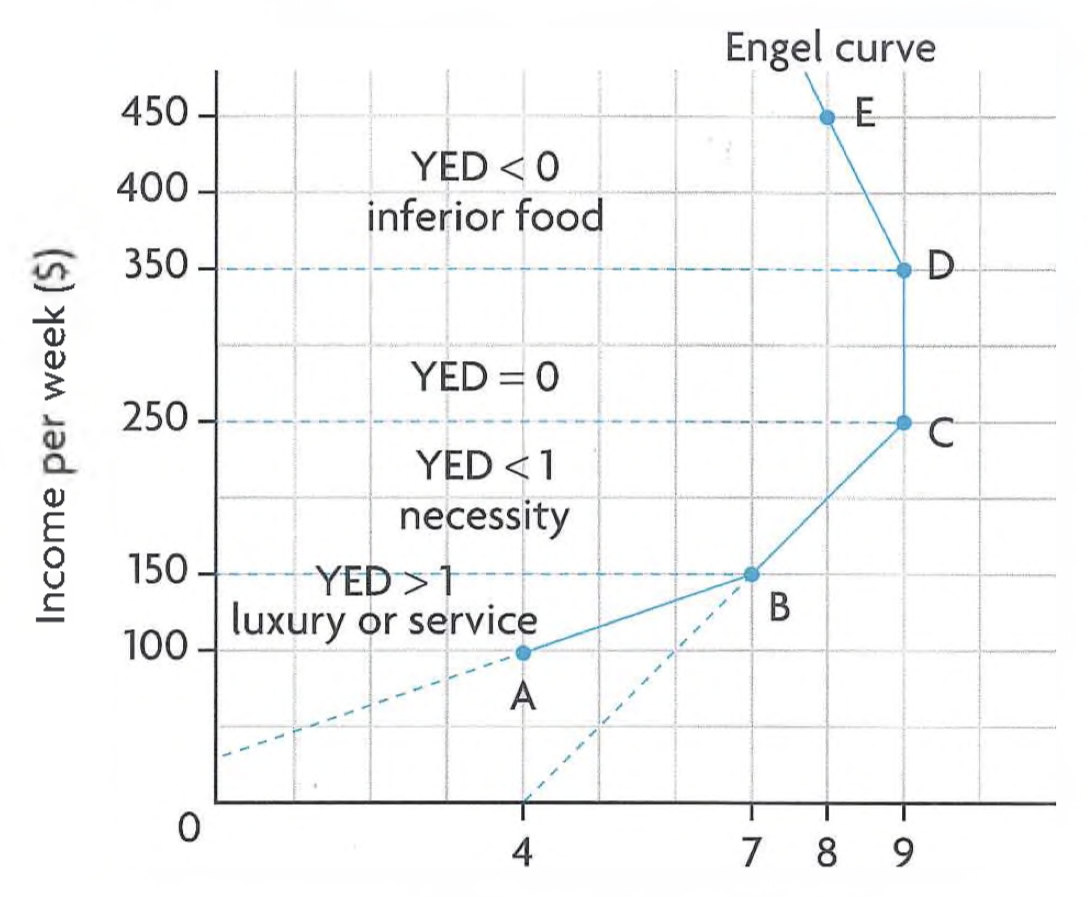
\includegraphics[width=0.45\linewidth]{Pasted 2026-07-16 at 09.46.47.png}
\end{center}
\begin{itemize}
  \item \textbf{Necessity} ($0 < YED < 1$): quantity demanded rises with income but at a \textit{decreasing} rate; the curve bends toward the income axis.
  \item \textbf{Luxury} ($YED > 1$): quantity demanded rises \textit{faster} than income; the curve steepens as income grows.
  \item \textbf{Inferior good} ($YED < 0$): quantity demanded initially rises but, beyond a critical income level $Y^*$, \textit{falls} as consumers switch to better alternatives; the curve bends backward.
\end{itemize}
The Engel curve shows a continuum: at very low incomes a good may be a luxury; as income increases it becomes a necessity and finally at high income levels it becomes inferior.
\[YED=\dfrac{\dfrac{\Delta Q}{Q}}{\dfrac{\Delta Y}{Y}}=\dfrac{\Delta Q}{\Delta Y}\times\dfrac{Y}{Q}=\dfrac{\dfrac{Y}{Q}}{\dfrac{\Delta Y}{\Delta Q}}\]
(YED then could be written as $\dfrac{k_\text{OX}}{k_\text{Engel}}$, $X\in\{A,B,C,D,E,...\}$. The numerical value of YED on each section depends on the relative size of the slope of the line segment.)
\subsubsection*{Applications of YED}
\begin{itemize}
    \item Estimation of the impact of changes in the business cycle, hence income, on different markets
  \item The rate of expansion of industries
  \begin{itemize}
    \item The higher the YED for a good or service, the greater the expansion of its market is likely to be in the future / the contraction in economic recessions.
    \item The lower the YED, the smaller the expansion / contraction (negative YED / inferior goods may even have increased demand in economic recession).
  \end{itemize}
  \item Sectoral structure of the economy
  \begin{itemize}
      \item Primary sector: agriculture, forestry, fishing and extractive industries
      \begin{itemize}
        \item Usually income inelastic
      \end{itemize}
      \item Secondary sector: manufacture goods from extracted raw material
      \begin{itemize}
        \item Usually income elastic
      \end{itemize}
      \item Tertiary sector: services sector (including entertainment, travel, banking, insurance, health care, education, and so on)
      \begin{itemize}
        \item Income elastic, YED greater than that of secondary sector products
      \end{itemize}
  \end{itemize}
\end{itemize}
Over time, the share of agricultural output in total output in the economy shrinks, while the share of manufactured output grows. With continued growth, the services sector expands at the expense of both agriculture and manufacturing.
\subsection{Supplementary: Cross-price elasticity of demand (XED)}
\needbold{Cross-price elasticity of demand (XED)} measures the responsiveness of the quantity demanded of good $X$ to a change in the price of good $Y$:
\[XED=\dfrac{\%\Delta Q_d(X)}{\%\Delta P(Y)}\]
\begin{itemize}
  \item $XED>0$: goods are \textbf{substitutes} (a rise in the price of $Y$ raises demand for $X$; e.g.\ Coke and Pepsi). The larger the positive value, the closer the substitutes.
  \item $XED<0$: goods are \textbf{complements} (a rise in the price of $Y$ lowers demand for $X$; e.g.\ cars and petrol). The larger the absolute value, the stronger the complementarity.
  \item $XED=0$: goods are \textbf{unrelated}.
\end{itemize}
Applications: helps firms identify actual competitors (relevant market definition); helps governments see the likely cross-market effects of taxes (e.g.\ taxing cigarettes raises demand for e-cigarettes if they are substitutes).
\subsection{Price elasticity of supply (PES)}
Price elasticity of supply is a measure of the responsiveness of the quantity of a good supplied to changes in its price. 
\begin{itemize}
  \item If there is a relatively large responsiveness of quantity supplied, supply is referred to as being elastic. ($PES>1$)
  \item If there is a relatively small responsiveness, supply is inelastic. ($PES<1$)
  \item Supply is unit elastic when $PES = 1$.
  \item Supply is perfectly inelastic when $PES = 0$.
  \item Supply is perfectly elastic when $PES =\infty$.
\end{itemize}
\[PES=\dfrac{\%\Delta Q_s}{\%\Delta P}=\dfrac{\dfrac{Q_2-Q_1}{Q_1}}{\dfrac{P_2-P_1}{P_1}}\]
\subsubsection*{Determinants of PES}
\begin{itemize}
  \item Length of time (to adjust resources and $Q_s$)
  \begin{itemize}
    \item Short time: highly inelastic
    \item Long time: elastic
  \end{itemize}
  \item Mobility of FoPs
  \begin{itemize}
    \item The more easily and quickly resources can be shifted out of one line of production and into another, PES is larger, supply is more elastic.
  \end{itemize}
  \item Spare / unused capacity of firms
  \begin{itemize}
    \item Larger spare capacity: PES larger, more elastic supply
    \item Lower / no spare capacity: PES smaller, more inelastic supply
  \end{itemize}
  \item Ability to store stocks
  \begin{itemize}
    \item Able to store stocks: High PES, more elastic supply
    \item Unable to store stocks: Low PES, more inelastic supply
  \end{itemize}
  \item Rate at which costs increase
  \begin{itemize}
    \item If the costs of producing extra output increase rapidly, then supply will be inelastic, PES would be small.
    \item If the costs of producing more output rise slowly, it will be easier for firms to expand their output so supply will be elastic, PES would be large.
  \end{itemize}
\end{itemize}
\subsubsection*{Applications of PES: PES in relation to primary commodities and manufactured products}
In general, primary commodities usually have a lower PES than manufactured products. The main reason
is the time needed for quantity supplied to respond to price changes. If put in a long-term scenario, the PES of the primary products would be more elastic that short-term scenarios. Inelastic supply of agricultural and other primary products also contributes to price and income instability for
primary product producers.
\section{Government intervention in microeconomics}
\subsection{Government intervention in markets}
\subsubsection*{Why government intervene in markets}
\begin{itemize}
  \item Earn revenue for the government (from indirect taxes, usually imposed on goods with inelastic demand)
  \item Provide support for firms (small firms / firms that government may want to encourage)
  \item Provide support to households on low incomes
  \item Influence the levels of production of firms
  \item Influence levels of consumption of individuals (encourage merit goods consumption, discourage demerit goods consumption)
  \item Correct market failure (failing to achieve allocative efficiency, overproduction / underproduction)
  \item Promote equity (equality) (through ways including income redistribution)
\end{itemize}
\subsubsection*{Forms of government intervention}
These are undertaken at a microeconomic level.
\begin{itemize}
  \item Price controls: Price ceilings / floors
  \item Indirect taxes
  \item Subsidies
  \item Direct provision of services
  \item Command and control regulation and legislation
  \item Consumer nudges
\end{itemize}
\subsection{Price controls}
Price controls refer to the setting of minimum or maximum prices by the government (or private organisations) so that prices are unable to adjust to their equilibrium level determined by demand and supply. Price controls result in market disequilibrium, and therefore in shortages 
(excess demand) or surpluses (excess supply).

\begin{center}
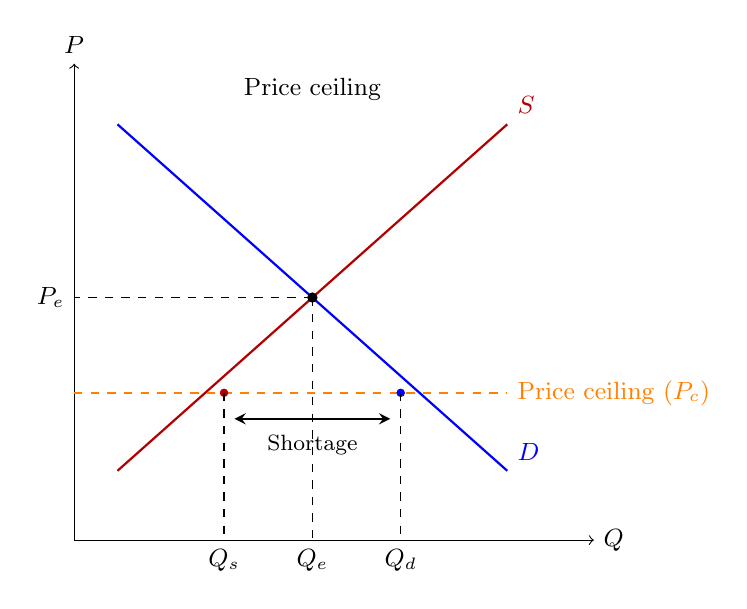
\begin{tikzpicture}[scale=1.1]
% --- Left: Price ceiling ---
\begin{scope}
\draw[->] (0,0) -- (6,0) node[right, font=\small] {$Q$};
\draw[->] (0,0) -- (0,5.5) node[above, font=\small] {$P$};
% Demand
\draw[thick, blue] (0.5,4.8) -- (5.0,0.8) node[above right, blue, font=\small] {$D$};
% Supply
\draw[thick, red!70!black] (0.5,0.8) -- (5.0,4.8) node[above right, red!70!black, font=\small] {$S$};
% Equilibrium
\filldraw (2.75,2.8) circle (1.5pt);
\draw[dashed] (2.75,2.8) -- (2.75,0) node[below, font=\small] {$Q_e$};
\draw[dashed] (2.75,2.8) -- (0,2.8) node[left, font=\small] {$P_e$};
% Price ceiling (below equilibrium)
\draw[thick, orange, dashed] (0,1.7) -- (5.0,1.7) node[right, orange, font=\small] {Price ceiling ($P_c$)};
% Qd and Qs at ceiling
\filldraw[blue] (3.77,1.7) circle (1.2pt);
\filldraw[red!70!black] (1.73,1.7) circle (1.2pt);
\draw[dashed] (3.77,1.7) -- (3.77,0) node[below, font=\small] {$Q_d$};
\draw[dashed] (1.73,1.7) -- (1.73,0) node[below, font=\small] {$Q_s$};
% Shortage bracket
\draw[<->, >=stealth, thick] (1.85,1.4) -- (3.65,1.4);
\node[font=\footnotesize] at (2.75,1.1) {Shortage};
\node[font=\small] at (2.75,5.2) {Price ceiling};
\end{scope}
\end{tikzpicture}
\end{center}
A \needbold{price ceiling} is a maximum price set below the equilibrium price, in order to make goods more affordable to people on low incomes. Examples: rent and food controls. Consequences of price ceilings:
\begin{itemize}
  \item For markets
  \begin{itemize}
    \item Creation of shortage $=Q_d-Q_s$
    \item Non-price rationing in order to distribute $Q_s$ among all interested buyers
    \item Underground / parallel markets (buying a good at legal max price, sell it at price higher than that)
    \item Underallocation of resources to the good (underproduction, $Q_s<Q_e$) and allocative inefficiency
    \item Negative welfare impacts: Welfare loss (also known as deadweight loss) represents social surplus or welfare benefits that are lost to society because resources are not allocated efficiently.

\begin{center}
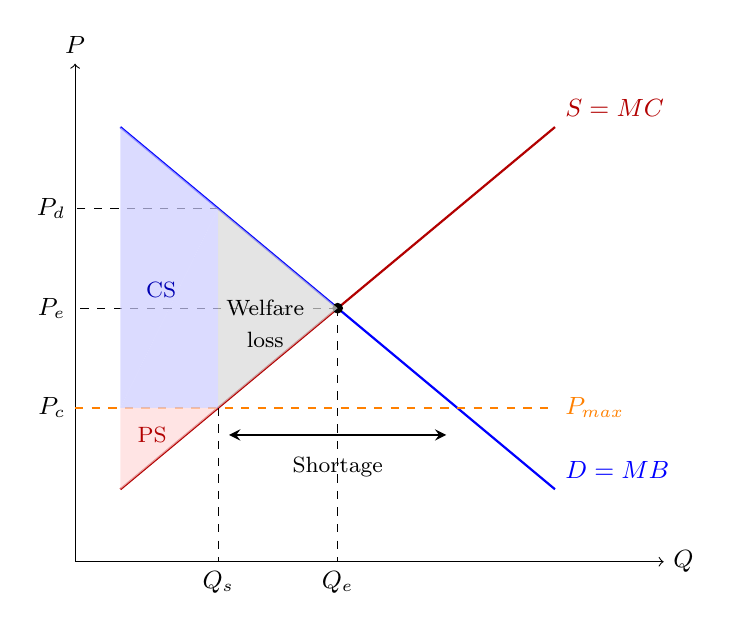
\begin{tikzpicture}[scale=1.15]
\draw[->] (0,0) -- (6.5,0) node[right, font=\small] {$Q$};
\draw[->] (0,0) -- (0,5.5) node[above, font=\small] {$P$};
% D = MB
\draw[thick, blue] (0.5,4.8) -- (5.3,0.8) node[above right, blue, font=\small] {$D = MB$};
% S = MC
\draw[thick, red!70!black] (0.5,0.8) -- (5.3,4.8) node[above right, red!70!black, font=\small] {$S = MC$};
% Equilibrium
\filldraw (2.9,2.8) circle (1.5pt);
\draw[dashed] (2.9,2.8) -- (2.9,0) node[below, font=\small] {$Q_e$};
\draw[dashed] (2.9,2.8) -- (0,2.8) node[left, font=\small] {$P_e$};
\node[left, font=\small] at (0,1.7) {$P_c$};
\node[left, font=\small] at (0,3.9) {$P_d$};
\draw[dashed] (1.58,3.9) -- (0,3.9);
% Price ceiling
\draw[thick, orange, dashed] (0,1.7) -- (5.3,1.7) node[right, orange, font=\small] {$P_{max}$};
% Qs at ceiling (on S curve): P=1.7, Q = 0.5 + (1.7-0.8)/4*4.8 = 0.5+1.08 = 1.58
% Qd at ceiling (on D curve): P=1.7, Q = 5.3 - (4.8-1.7)/4*4.8 = 5.3-0.775*4.8 ... let me compute directly
% D: P = 4.8 - (4/4.8)(Q-0.5), at P=1.7: 1.7=4.8-0.833(Q-0.5), 3.1=0.833(Q-0.5), Q=0.5+3.72=4.22
% S: P = 0.8 + (4/4.8)(Q-0.5), at P=1.7: 0.9=0.833(Q-0.5), Q=0.5+1.08=1.58
% Actual quantity transacted = Qs = 1.58
\draw[dashed] (1.58,1.7) -- (1.58,0) node[below, font=\small] {$Q_s$};
% Consumer surplus: triangle above P_max, below D, up to Qs
% At Qs=1.58, D height = 1.7; D intercept = 4.8
\fill[blue!20, opacity=0.7] (0.5,4.8) -- (1.58,3.9) -- (0.5,1.7) -- cycle;
\fill[blue!20, opacity=0.7] (0.5,1.7) -- (1.58,1.7) -- (1.58,3.9) -- cycle;
\node[blue!70!black, font=\footnotesize] at (0.95,3.0) {CS};
% Producer surplus: triangle below P_max, above S, up to Qs
\fill[red!15, opacity=0.7] (0.5,0.8) -- (1.58,1.7) -- (0.5,1.7) -- cycle;
\node[red!70!black, font=\footnotesize] at (0.85,1.4) {PS};
% Welfare loss (deadweight loss): triangle between D and S, from Qs to Qe
\fill[gray!30, opacity=0.7] (1.58,3.9) -- (1.58,1.7) -- (2.9,2.8) -- cycle;
\node[font=\footnotesize] at (2.1,2.8) {Welfare};
\node[font=\footnotesize] at (2.1,2.45) {loss};
% Shortage bracket
\draw[<->, >=stealth, thick] (1.7,1.4) -- (4.1,1.4);
\node[font=\footnotesize] at (2.9,1.05) {Shortage};
% P_max label on axis
\node[left, font=\small] at (0,1.7) {};
\end{tikzpicture}
\end{center}
At the price ceiling $P_{max}$, only $Q_s$ is supplied (and transacted). \textbf{Consumer surplus (CS)} is the area above $P_{max}$ and below the $D=MB$ curve up to $Q_s$. \textbf{Producer surplus (PS)} is the area below $P_{max}$ and above the $S=MC$ curve up to $Q_s$. The shaded triangle between $Q_s$ and $Q_e$ is the \textbf{welfare loss (deadweight loss)} --- output that would have benefited society ($MB > MC$) is not produced due to the price ceiling.
  \end{itemize}
  \item For stakeholders
  \begin{itemize}
    \item Consumers: some consumers are able to buy the good at the lower price are better off. However, some consumers remain unsatisfied since they don't get to buy the good at all.
    \item Producers: worse off, they sell a lower quantity of goods at a lower price, resulting in decreased revenue.
    \item Workers: resulting in unemployment
  \end{itemize}
\end{itemize}
\subsubsection*{Calculating the effects of price ceilings on stakeholders and welfare}
Change in consumer spending / firm revenue: $P_e\times Q_e-P_c\times Q_s$.\\
Change in consumer and producer welfare and welfare loss:
\[\Delta \text{Consumer surplus}=\dfrac{1}{2}Q_e\times (P_\text{intercept of D}-P_e)-\dfrac{1}{2}Q_s\times((P_d-P_c)+(P_\text{intercept of D}-P_c))\]
\[\Delta \text{Producer surplus}=\dfrac{1}{2}Q_e\times(P_e-P_\text{intercept of S})-\dfrac{1}{2}(P_e-P_c)\times (Q_s+Q_e)\]
\[\text{Welfare loss}=-(\Delta \text{Consumer surplus}+\Delta \text{Producer surplus})=\dfrac{1}{2}(P_d-P_c)\times (Q_e-Q_s)\]
\begin{center}
  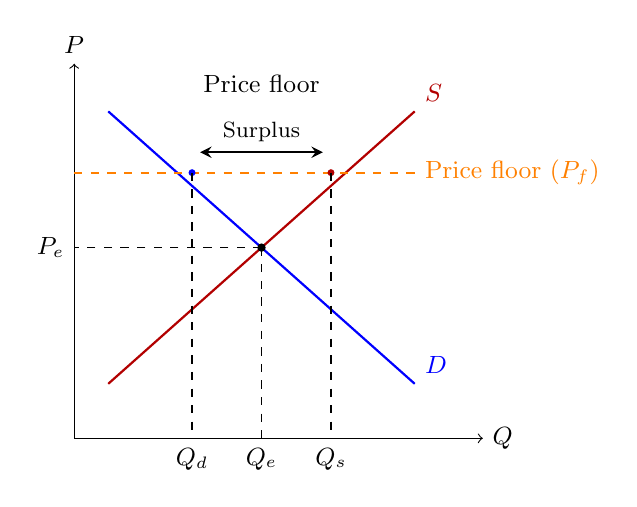
\begin{tikzpicture}[scale=0.865]
  % --- Right: Price floor ---
\begin{scope}[xshift=8cm]
\draw[->] (0,0) -- (6,0) node[right, font=\small] {$Q$};
\draw[->] (0,0) -- (0,5.5) node[above, font=\small] {$P$};
% Demand
\draw[thick, blue] (0.5,4.8) -- (5.0,0.8) node[above right, blue, font=\small] {$D$};
% Supply
\draw[thick, red!70!black] (0.5,0.8) -- (5.0,4.8) node[above right, red!70!black, font=\small] {$S$};
% Equilibrium
\filldraw (2.75,2.8) circle (1.5pt);
\draw[dashed] (2.75,2.8) -- (2.75,0) node[below, font=\small] {$Q_e$};
\draw[dashed] (2.75,2.8) -- (0,2.8) node[left, font=\small] {$P_e$};
% Price floor (above equilibrium)
\draw[thick, orange, dashed] (0,3.9) -- (5.0,3.9) node[right, orange, font=\small] {Price floor ($P_f$)};
% Qd and Qs at floor
\filldraw[blue] (1.73,3.9) circle (1.2pt);
\filldraw[red!70!black] (3.77,3.9) circle (1.2pt);
\draw[dashed] (1.73,3.9) -- (1.73,0) node[below, font=\small] {$Q_d$};
\draw[dashed] (3.77,3.9) -- (3.77,0) node[below, font=\small] {$Q_s$};
% Surplus bracket
\draw[<->, >=stealth, thick] (1.85,4.2) -- (3.65,4.2);
\node[font=\footnotesize] at (2.75,4.5) {Surplus};
\node[font=\small] at (2.75,5.2) {Price floor};
\end{scope}
\end{tikzpicture}
\end{center}
A \needbold{price floor} is a minimum price set above the equilibrium price, in order to provide income support to farmers or to increase the wages of low-skilled workers. Consequences of price floors:
\begin{itemize}
  \item For markets
  \begin{itemize}
    \item Creation of surplus: $Q_s-Q_d$
    \item A common practice is for the government to buy the excess supply, and this causes the demand curve for the product to shift to the right.

\begin{center}
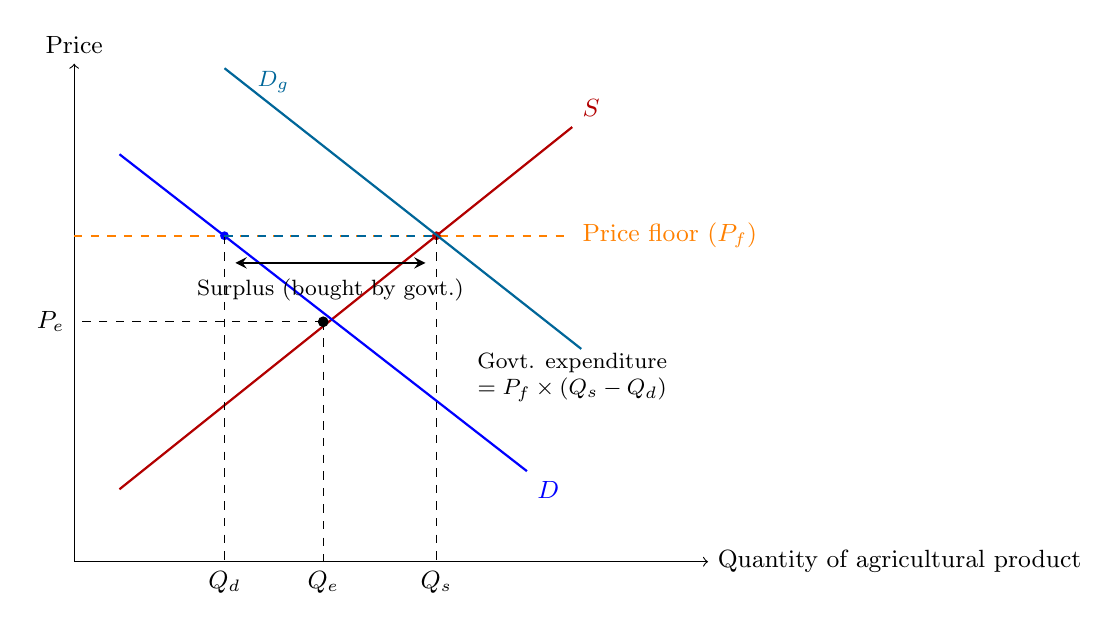
\begin{tikzpicture}[scale=1.15]
\draw[->] (0,0) -- (7,0) node[right, font=\small] {Quantity of agricultural product};
\draw[->] (0,0) -- (0,5.5) node[above, font=\small] {Price};
% Supply S
\draw[thick, red!70!black] (0.5,0.8) -- (5.5,4.8) node[above right, red!70!black, font=\small] {$S$};
% Original demand D
\draw[thick, blue] (0.5,4.5) -- (5.0,1.0) node[below right, blue, font=\small] {$D$};
% Equilibrium (no intervention)
\filldraw (2.75,2.65) circle (1.5pt);
\draw[dashed] (2.75,2.65) -- (2.75,0) node[below, font=\small] {$Q_e$};
\draw[dashed] (2.75,2.65) -- (0,2.65) node[left, font=\small] {$P_e$};
% Price floor
\draw[thick, orange, dashed] (0,3.6) -- (5.5,3.6) node[right, orange, font=\small] {Price floor ($P_f$)};
% Qd on original D at Pf: P=3.6, D: P=4.5-3.5/4.5*(Q-0.5), 3.6=4.5-0.778(Q-0.5), 0.9=0.778(Q-0.5), Q=1.657
\filldraw[blue] (1.66,3.6) circle (1.2pt);
\draw[dashed] (1.66,3.6) -- (1.66,0) node[below, font=\small] {$Q_d$};
% Qs on S at Pf: P=3.6, S: P=0.8+4/5*(Q-0.5), 3.6=0.8+0.8(Q-0.5), 2.8=0.8(Q-0.5), Q=4.0
\filldraw[red!70!black] (4.0,3.6) circle (1.2pt);
\draw[dashed] (4.0,3.6) -- (4.0,0) node[below, font=\small] {$Q_s$};
% Government demand D_g (horizontal at Pf from Qd to Qs, then up along D)
% New effective demand: D from 0.5 to Qd, then horizontal at Pf to Qs
\draw[thick, blue!60!green, dashed] (1.66,3.6) -- (4.0,3.6);
\node[blue!60!green, font=\footnotesize] at (2.2,5.3) {$D_g$};
\draw[thick, blue!60!green] (1.66, 5.45) -- (5.6,2.35);
% Surplus label
\draw[<->, >=stealth, thick] (1.78,3.3) -- (3.88,3.3);
\node[font=\footnotesize] at (2.83,3.0) {Surplus (bought by govt.)};
% Government expenditure
\node[font=\footnotesize] at (5.5,2.2) {Govt. expenditure};
\node[font=\footnotesize] at (5.5,1.9) {$= P_f \times (Q_s - Q_d)$};
\end{tikzpicture}
\end{center}
    \item The government must make a decision about what to do with the surplus: store / export?
    \item Firm inefficiency: inefficient firms with high costs of production do not face incentives to cut costs because the high price offers them protection against lower-cost competitors.
    \item Overallocation of resources to the production of the good and allocative inefficiency
    \item Negative welfare impacts:

\begin{center}
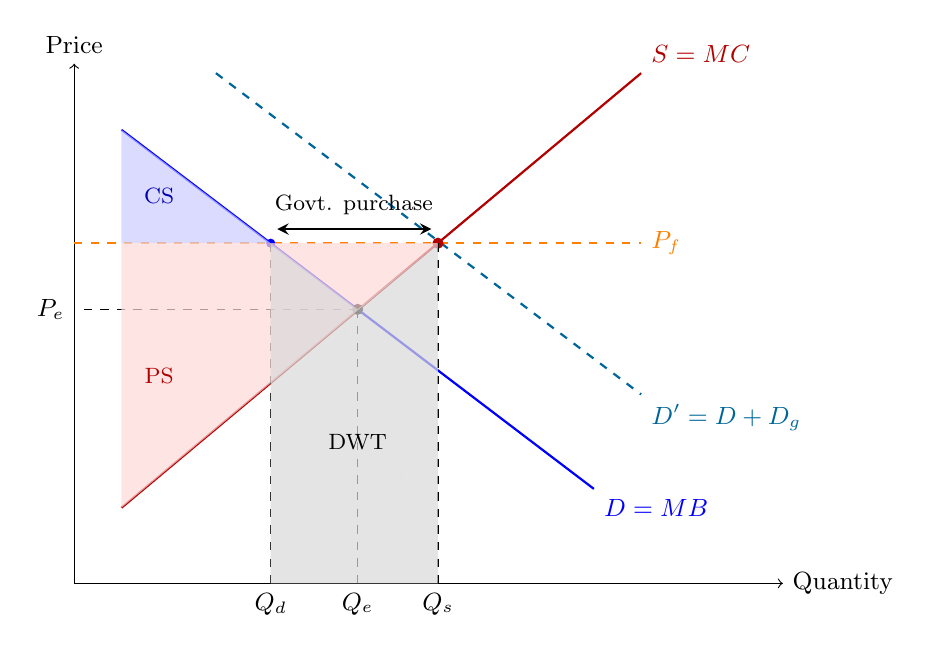
\begin{tikzpicture}[scale=1.2]
\draw[->] (0,0) -- (7.5,0) node[right, font=\small] {Quantity};
\draw[->] (0,0) -- (0,5.5) node[above, font=\small] {Price};
% S = MC
\draw[thick, red!70!black] (0.5,0.8) -- (6.0,5.4) node[above right, red!70!black, font=\small] {$S = MC$};
% D = MB (original demand)
\draw[thick, blue] (0.5,4.8) -- (5.5,1.0) node[below right, blue, font=\small] {$D = MB$};
% D' = MB + govt purchase (rightward shifted)
\draw[thick, blue!60!green, dashed] (1.5,5.4) -- (6.0,2.0) node[below right, blue!60!green, font=\small] {$D' = D + D_g$};
% Original equilibrium (D intersect S)
\filldraw (3.0,2.9) circle (1.5pt);
\draw[dashed] (3.0,2.9) -- (3.0,0) node[below, font=\small] {$Q_e$};
\draw[dashed] (3.0,2.9) -- (0,2.9) node[left, font=\small] {$P_e$};
% Price floor
\draw[thick, orange, dashed] (0,3.6) -- (6.0,3.6) node[right, orange, font=\small] {$P_f$};
% Qd on original D at Pf
\filldraw[blue] (2.08,3.6) circle (1.2pt);
\draw[dashed] (2.08,3.6) -- (2.08,0) node[below, font=\small] {$Q_d$};
% Qs: D' intersect S
\filldraw[red!70!black] (3.85,3.6) circle (1.5pt);
\draw[dashed] (3.85,3.6) -- (3.85,0) node[below, font=\small] {$Q_s$};
% Consumer surplus
\fill[blue!20, opacity=0.7] (0.5,4.8) -- (2.08,3.6) -- (0.5,3.6) -- cycle;
\node[blue!70!black, font=\footnotesize] at (0.9,4.1) {CS};
% Producer surplus
% \fill[red!15, opacity=0.7] (0.5,0.8) -- (2.08,2.1) -- (0.5,3.6) -- cycle;
% \fill[red!15, opacity=0.7] (2.08,3.6) -- (2.08,2.1) -- (0.5,3.6) -- cycle;
\fill[red!15, opacity=0.7] (0.5,0.8) -- (3.85,3.6) -- (0.5,3.6) -- cycle;
\node[red!70!black, font=\footnotesize] at (0.9,2.2) {PS};
% Welfare loss triangle
\fill[gray!30, opacity=0.7] (2.08,3.6) -- (3.0,2.9) -- (2.08,0) -- cycle;
\fill[gray!30, opacity=0.7] (2.08,0) -- (3.85,0) -- (3.0,2.9) -- cycle;
\fill[gray!30, opacity=0.7] (3.85,0) -- (3.0,2.9) -- (3.85,3.6) -- cycle;
\node[font=\footnotesize] at (3,1.5) {DWT};
% Surplus bought by government
\draw[<->, >=stealth, thick] (2.15,3.75) -- (3.78,3.75);
\node[font=\footnotesize] at (2.96,4) {Govt. purchase};
\end{tikzpicture}
\end{center}
Government spending to maintain the price floor involves losses for society. The grey shaded area is the DWT (while the producers gain the additional red triangle, the government pays a price of the grey rectangle) $MB<MC$, indicating that society would be better off if less of the good were produced.
\end{itemize}
  \item For stakeholders
  \begin{itemize}
    \item Consumers: worse off, pay a higher price for the good
    \item Producers: better, gain as they receive a higher price and produce a larger quantity
    \item Workers: employment increases
    \item Government: a burden on its budget, also incur OPC
  \end{itemize}
\end{itemize}
\subsubsection*{Calculating effects of price floors on stakeholders and social welfare}
Changes in consumer expenditure: $P_f\times Q_d-P_e\times Q_e$\\
Changes in producer revenue: $P_f\times Q_s-P_e\times Q_e$\\
Changes in government expenditure: $P_f\times (Q_s-Q_d)$
\[\Delta \text{Consumer surplus}=\dfrac{1}{2}(Q_d+Q_e)\times (P_f-P_e)\]
\[\Delta \text{Producer surplus}=\dfrac{1}{2}(Q_e+Q_s)\times (P_f-P_e)\]
\[\Delta \text{Welfare loss}=(Q_s-Q_d)\times P_f-\dfrac{1}{2}(Q_s-Q_d)\times (P_f-P_e)\]
\subsubsection*{Minimum wages}

\begin{center}
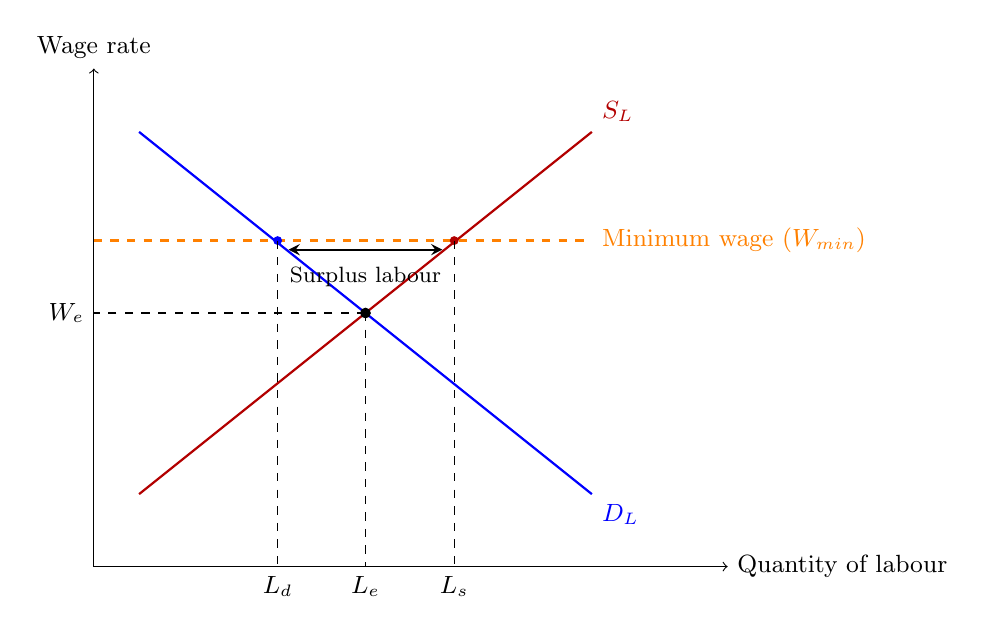
\begin{tikzpicture}[scale=1.15]
\draw[->] (0,0) -- (7,0) node[right, font=\small] {Quantity of labour};
\draw[->] (0,0) -- (0,5.5) node[above, font=\small] {Wage rate};
% Supply of labour S_L (upward sloping)
\draw[thick, red!70!black] (0.5,0.8) -- (5.5,4.8) node[above right, red!70!black, font=\small] {$S_L$};
% Demand for labour D_L (downward sloping)
\draw[thick, blue] (0.5,4.8) -- (5.5,0.8) node[below right, blue, font=\small] {$D_L$};
% Equilibrium
\filldraw (3.0,2.8) circle (1.5pt);
\draw[dashed] (3.0,2.8) -- (3.0,0) node[below, font=\small] {$L_e$};
\draw[dashed] (3.0,2.8) -- (0,2.8) node[left, font=\small] {$W_e$};
% Minimum wage (above equilibrium)
\draw[thick, orange, dashed] (0,3.6) -- (5.5,3.6) node[right, orange, font=\small] {Minimum wage ($W_{min}$)};
% Quantity of labour demanded at Wmin
\filldraw[blue] (2.03,3.6) circle (1.2pt);
\draw[dashed] (2.03,3.6) -- (2.03,0) node[below, font=\small] {$L_d$};
% Quantity of labour supplied at Wmin
\filldraw[red!70!black] (3.98,3.6) circle (1.2pt);
\draw[dashed] (3.98,3.6) -- (3.98,0) node[below, font=\small] {$L_s$};
% Surplus labour bracket
\draw[<->, >=stealth, thick] (2.15,3.5) -- (3.85,3.5);
\node[font=\footnotesize] at (3.0,3.2) {Surplus labour};
\end{tikzpicture}
\end{center}
A \needbold{minimum wage} ($W_{min}$) is a price floor in the labour market, set above the equilibrium wage $W_e$. Consequences of minimum wages:
\begin{itemize}
  \item Labour surplus (excess supply) and unemployment
  \item Illegal workers at wages below the minimum wage
  \item Misallocation of labour resources
  \item Misallocation in product markets
\end{itemize}
Consequences for various stakeholders:
\begin{itemize}
  \item Firms: worse off, increase CoP
  \item Workers: some receive higher wages, some experience unemployment
  \item Consumers: extra CoP reflected in higher prices
\end{itemize}
The level of unemployment created largely depends on the minimum wage set. It may even increase labor productivity due to an increase in incentive for work.
\subsubsection*{Setting fixed prices}
Sometimes prices may be fixed at a particular level by the government (e.g.\ tickets for a sports event with a fixed number of seats). The supply curve is \textbf{vertical}. If the fixed price is set below the equilibrium, it creates a \textbf{shortage}; if set above, it creates a \textbf{surplus}.

\begin{center}
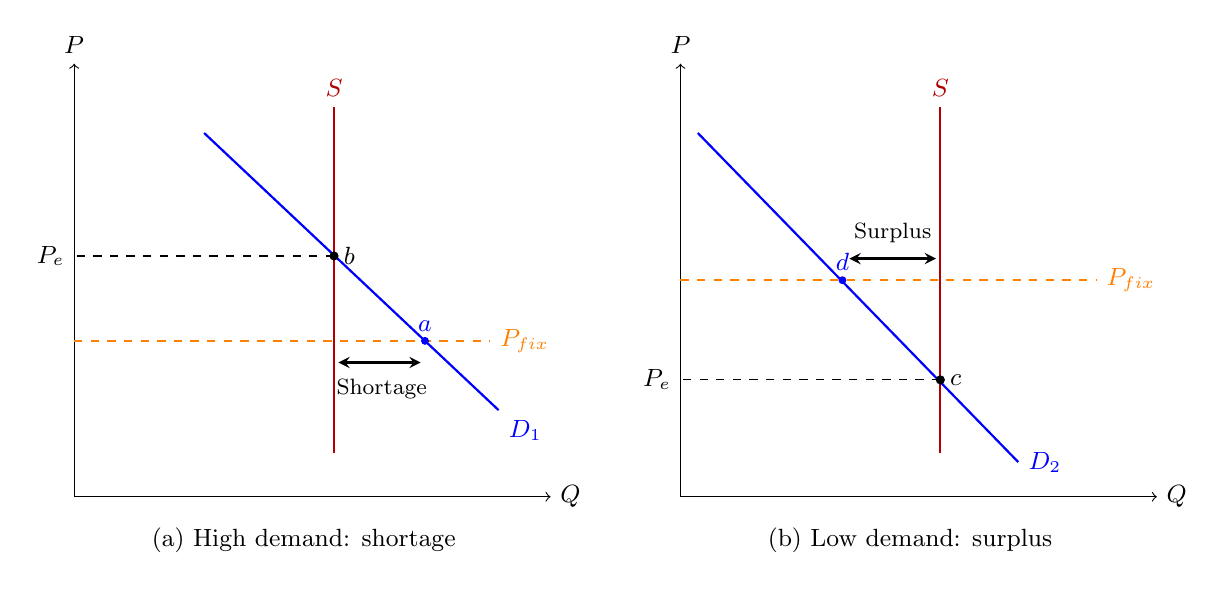
\begin{tikzpicture}[scale=1.1]
% --- Left: high demand, fixed price below equilibrium -> shortage ---
\begin{scope}
\draw[->] (0,0) -- (5.5,0) node[right, font=\small] {$Q$};
\draw[->] (0,0) -- (0,5) node[above, font=\small] {$P$};
% Vertical supply at Q=3
\draw[thick, red!70!black] (3.0,0.5) -- (3.0,4.5) node[above, red!70!black, font=\small] {$S$};
% High demand D1
\draw[thick, blue] (1.5,4.2) -- (4.9,1.0) node[below right, blue, font=\small] {$D_1$};
% Equilibrium (D1 intersects S at Q=3)
\filldraw (3.0,2.78) circle (1.3pt) node[right, font=\small] {$b$};
\draw[dashed] (3.0,2.78) -- (0,2.78) node[left, font=\small] {$P_e$};
% Fixed price below equilibrium
\draw[thick, orange, dashed] (0,1.8) -- (4.8,1.8) node[right, orange, font=\small] {$P_{fix}$};
% Qd at Pfix on D1
\filldraw[blue] (4.05,1.8) circle (1.1pt) node[above, font=\small] {$a$};
% Shortage bracket
\draw[<->, >=stealth, thick] (3.05,1.55) -- (4.0,1.55);
\node[font=\footnotesize] at (3.55,1.25) {Shortage};
\node[font=\small] at (2.65,-0.5) {(a) High demand: shortage};
\end{scope}
% --- Right: low demand, fixed price above equilibrium -> surplus ---
\begin{scope}[xshift=7cm]
\draw[->] (0,0) -- (5.5,0) node[right, font=\small] {$Q$};
\draw[->] (0,0) -- (0,5) node[above, font=\small] {$P$};
% Vertical supply at Q=3
\draw[thick, red!70!black] (3.0,0.5) -- (3.0,4.5) node[above, red!70!black, font=\small] {$S$};
% Low demand D2
\draw[thick, blue] (0.2,4.2) -- (3.9,0.4) node[right, blue, font=\small] {$D_2$};
% Equilibrium (D2 intersects S at Q=3)
\filldraw (3.0,1.35) circle (1.3pt) node[right, font=\small] {$c$};
\draw[dashed] (3.0,1.35) -- (0,1.35) node[left, font=\small] {$P_e$};
% Fixed price above equilibrium
\draw[thick, orange, dashed] (0,2.5) -- (4.8,2.5) node[right, orange, font=\small] {$P_{fix}$};
% Qd at Pfix on D2
\filldraw[blue] (1.87,2.5) circle (1.1pt) node[above, font=\small] {$d$};
% Surplus bracket
\draw[<->, >=stealth, thick] (1.95,2.75) -- (2.95,2.75);
\node[font=\footnotesize] at (2.45,3.05) {Surplus};
\node[font=\small] at (2.65,-0.5) {(b) Low demand: surplus};
\end{scope}
\end{tikzpicture}
\end{center}
\subsection{Indirect taxes}
\needbold{Indirect taxes} are imposed on spending to buy goods and services. Types of indirect tax include:
\begin{itemize}
  \item excise taxes, imposed on particular goods and services, such as petrol, cigarettes and alcohol
  \item taxes on spending on all (or most) goods and services, such as general sales taxes and value added taxes.
\end{itemize}
Why do governments impose excise taxes?
\begin{itemize}
  \item Indirect taxes are a source of government revenue.
  \item Indirect taxes are a method to discourage consumption of goods that are harmful for the individual.
  \item Indirect taxes can be used to redistribute income.
  \item Indirect taxes are a method to improve the allocation of resources (reduce allocative inefficiencies) by correcting negative externalities.
\end{itemize}
Indirect, excise taxes can be:
\begin{itemize}
  \item \needbold{specific taxes}, a fixed amount of tax per unit of the good or service sold;
  \item \needbold{ad valorem taxes}, a fixed percentage of the price of the good or service.
\end{itemize}
\begin{center}
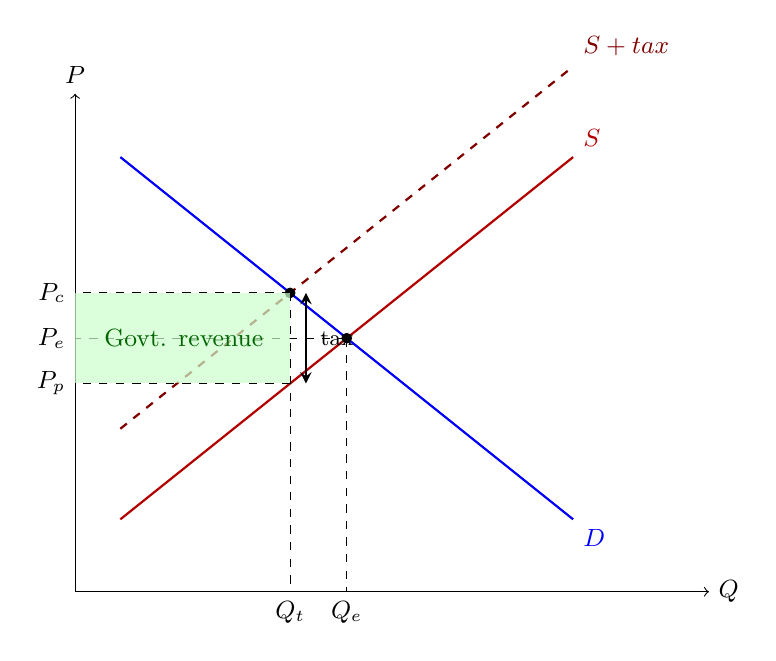
\begin{tikzpicture}[scale=1.15]
\draw[->] (0,0) -- (7,0) node[right, font=\small] {$Q$};
\draw[->] (0,0) -- (0,5.5) node[above, font=\small] {$P$};
% Original supply S
\draw[thick, red!70!black] (0.5,0.8) -- (5.5,4.8) node[above right, red!70!black, font=\small] {$S$};
% New supply S + tax (parallel shift upward)
\draw[thick, red!50!black, dashed] (0.5,1.8) -- (5.5,5.8) node[above right, red!50!black, font=\small] {$S + tax$};
% Demand D
\draw[thick, blue] (0.5,4.8) -- (5.5,0.8) node[below right, blue, font=\small] {$D$};
% Original equilibrium
\filldraw (3.0,2.8) circle (1.5pt);
\draw[dashed] (3.0,2.8) -- (3.0,0) node[below, font=\small] {$Q_e$};
\draw[dashed] (3.0,2.8) -- (0,2.8) node[left, font=\small] {$P_e$};
% New equilibrium (D intersects S+tax)
% S+tax: P = 1.8 + 4/5*(Q-0.5); D: P = 4.8 - 4/5*(Q-0.5)
% 1.8+0.8(Q-0.5) = 4.8-0.8(Q-0.5), 1.6(Q-0.5)=3.0, Q-0.5=1.875, Q=2.375
\filldraw (2.375,3.3) circle (1.5pt);
\draw[dashed] (2.375,3.3) -- (2.375,0) node[below, font=\small] {$Q_t$};
% Price paid by consumers Pc
\draw[dashed] (2.375,3.3) -- (0,3.3) node[left, font=\small] {$P_c$};
% Price received by producers Pp (on original S at Qt)
% S at Q=2.375: P = 0.8+0.8(1.875) = 0.8+1.5 = 2.3
\draw[dashed] (2.375,2.3) -- (0,2.3) node[left, font=\small] {$P_p$};
% Government revenue: rectangle (Pc - Pp) * Qt
\fill[green!20, opacity=0.7] (0,2.3) rectangle (2.375,3.3);
\node[green!40!black, font=\small] at (1.2,2.8) {Govt. revenue};
% Tax wedge label
\draw[<->, >=stealth, thick] (2.55,2.3) -- (2.55,3.3);
\node[font=\footnotesize, right] at (2.6,2.8) {tax};
\end{tikzpicture}
\end{center}
An indirect (excise) tax shifts the supply curve \textbf{upward} from $S$ to $S + tax$. The new equilibrium has a \textbf{lower quantity} $Q_t < Q_e$. Consumers pay a \textbf{higher price} $P_c$; producers receive a \textbf{lower price} $P_p$ (after paying the tax). The green rectangle $= (P_c - P_p) \times Q_t$ is the \textbf{government tax revenue}.
Consequences of indirect taxes for various stakeholders:
\begin{itemize}
  \item Consumers: Increase in price, decrease in quantity bought
  \item Firms: fall of output and fall of revenue they receive (decreased price)
  \item Governments: Gains revenue
  \item Workers: leads to some unemployment
  \item Society as a whole: CS, PS, DWT\\
  In this case, welfare loss appears because the tax causes a smaller than optimum quantity to be produced, which is an indication of underproduction.
\end{itemize}

\begin{center}
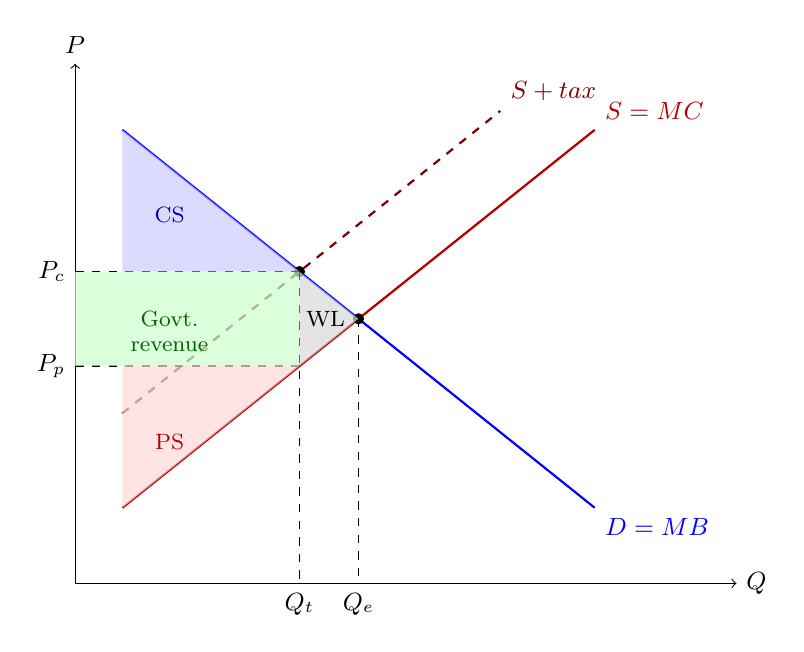
\begin{tikzpicture}[scale=1.2]
\draw[->] (0,0) -- (7,0) node[right, font=\small] {$Q$};
\draw[->] (0,0) -- (0,5.5) node[above, font=\small] {$P$};
% S = MC
\draw[thick, red!70!black] (0.5,0.8) -- (5.5,4.8) node[above right, red!70!black, font=\small] {$S = MC$};
% S + tax (parallel shift up by 1 unit)
\draw[thick, red!50!black, dashed] (0.5,1.8) -- (4.5,5.0) node[above right, red!50!black, font=\small] {$S + tax$};
% D = MB
\draw[thick, blue] (0.5,4.8) -- (5.5,0.8) node[below right, blue, font=\small] {$D = MB$};
% Original equilibrium
\filldraw (3.0,2.8) circle (1.5pt);
\draw[dashed] (3.0,2.8) -- (3.0,0) node[below, font=\small] {$Q_e$};
% New equilibrium (D intersects S+tax): Q=2.375
\filldraw (2.375,3.3) circle (1.5pt);
\draw[dashed] (2.375,3.3) -- (2.375,0) node[below, font=\small] {$Q_t$};
% Pc and Pp
\draw[dashed] (2.375,3.3) -- (0,3.3) node[left, font=\small] {$P_c$};
\draw[dashed] (2.375,2.3) -- (0,2.3) node[left, font=\small] {$P_p$};
% Consumer surplus: above Pc, below D, up to Qt
\fill[blue!20, opacity=0.7] (0.5,4.8) -- (2.375,3.3) -- (0.5,3.3) -- cycle;
\node[blue!70!black, font=\footnotesize] at (1.0,3.9) {CS};
% Producer surplus: below Pp, above S, up to Qt
\fill[red!15, opacity=0.7] (0.5,0.8) -- (2.375,2.3) -- (0.5,2.3) -- cycle;
\node[red!70!black, font=\footnotesize] at (1.0,1.5) {PS};
% Government revenue: rectangle (Pc - Pp) * Qt
\fill[green!20, opacity=0.7] (0,2.3) rectangle (2.375,3.3);
\node[green!40!black, font=\footnotesize] at (1.0,2.8) {Govt.};
\node[green!40!black, font=\footnotesize] at (1.0,2.5) {revenue};
% Welfare loss: triangle between D(MB) and S(MC) from Qt to Qe
\fill[gray!30, opacity=0.7] (2.375,3.3) -- (3.0,2.8) -- (2.375,2.3) -- cycle;
\node[font=\footnotesize] at (2.65,2.8) {WL};
\end{tikzpicture}
\end{center}
\subsubsection*{Calculating the effects of indirect taxes on stakeholders and social welfare}
Change in consumer expenditure: $P_e\times Q_e-P_c\times Q_t$\\
Change in producer revenue: $P_e\times Q_e-P_p\times Q_t$\\
Government revenue: $(P_c-P_p)\times Q_t$\\
Change in CS: $\dfrac{1}{2}(P_\text{intercept of D}-P_e)\times Q_e-\dfrac{1}{2}(P_\text{intercept of D}-P_c)\times Q_t$\\
Change in PS: $\dfrac{1}{2}(P_e-P_\text{intercept of S})\times Q_e-\dfrac{1}{2}(P_p-P_\text{intercept of S})\times Q_t$\\
DWT / welfare loss: $\dfrac{1}{2}(P_c-P_p)\times(Q_e-Q_t)$
\subsubsection*{Tax incidence and price elasticities of demand and supply}
\textbf{Tax incidence} refers to the distribution of the burden of a tax between consumers and producers. When a good is taxed, consumers pay a higher price ($P_c > P_e$) and producers receive a lower price ($P_p < P_e$). The total tax revenue $= (P_c - P_p) \times Q_t$ is shared between the two groups:
\begin{itemize}
  \item \textbf{Tax burden on consumers} $= (P_c - P_e) \times Q_t$
  \item \textbf{Tax burden on producers} $= (P_e - P_p) \times Q_t$
\end{itemize}
The distribution depends on \textbf{PED and PES}:
\begin{itemize}
  \item \textbf{Inelastic demand} (steep $D$): consumers are unresponsive to price changes, so they bear \textbf{most} of the tax burden. The drop in quantity ($Q_e \to Q_t$) is small.
  \item \textbf{Elastic demand} (flat $D$): consumers are responsive and can easily switch to substitutes, so producers bear \textbf{most} of the tax burden. The drop in quantity is larger.
\end{itemize}
Similarly for \textbf{PES}:
\begin{itemize}
  \item \textbf{Inelastic supply} (steep $S$): producers bear most of the tax burden.
  \item \textbf{Elastic supply} (flat $S$): consumers bear most of the tax burden.
\end{itemize}

\begin{center}
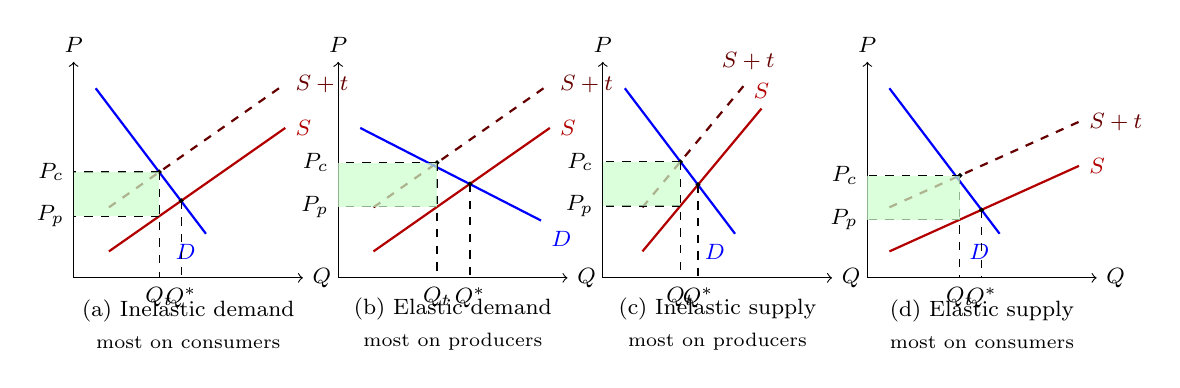
\begin{tikzpicture}[scale=0.56]
% (a) Inelastic demand
\begin{scope}
\draw[->] (0,0) -- (5.2,0) node[right, font=\footnotesize] {$Q$};
\draw[->] (0,0) -- (0,4.9) node[above, font=\footnotesize] {$P$};
\draw[thick, red!70!black] (0.8,0.6) -- (4.8,3.4) node[right, red!70!black, font=\footnotesize] {$S$};
\draw[thick, red!40!black, dashed] (0.8,1.6) -- (4.8,4.4) node[right, red!40!black, font=\footnotesize] {$S+t$};
\draw[thick, blue] (0.5,4.3) -- (3.0,1.0) node[below left, blue, font=\footnotesize] {$D$};
\filldraw (2.44,1.75) circle (1.2pt);
\filldraw (1.94,2.40) circle (1.2pt);
\draw[dashed] (2.44,1.75) -- (2.44,0) node[below, font=\footnotesize] {$Q^*$};
\draw[dashed] (1.94,2.40) -- (1.94,0) node[below, font=\footnotesize] {$Q_t$};
\draw[dashed] (1.94,2.40) -- (0,2.40) node[left, font=\footnotesize] {$P_c$};
\draw[dashed] (1.94,1.40) -- (0,1.40) node[left, font=\footnotesize] {$P_p$};
\fill[green!20, opacity=0.7] (0,1.40) rectangle (1.94,2.40);
\node[font=\footnotesize, align=center] at (2.6,-1.05) {(a) Inelastic demand\\[2pt]{\scriptsize most on consumers}};
\end{scope}
% (b) Elastic demand
\begin{scope}[xshift=6.0cm]
\draw[->] (0,0) -- (5.2,0) node[right, font=\footnotesize] {$Q$};
\draw[->] (0,0) -- (0,4.9) node[above, font=\footnotesize] {$P$};
\draw[thick, red!70!black] (0.8,0.6) -- (4.8,3.4) node[right, red!70!black, font=\footnotesize] {$S$};
\draw[thick, red!40!black, dashed] (0.8,1.6) -- (4.8,4.4) node[right, red!40!black, font=\footnotesize] {$S+t$};
\draw[thick, blue] (0.5,3.4) -- (4.6,1.3) node[below right, blue, font=\footnotesize] {$D$};
\filldraw (2.99,2.13) circle (1.2pt);
\filldraw (2.24,2.61) circle (1.2pt);
\draw[dashed] (2.99,2.13) -- (2.99,0) node[below, font=\footnotesize] {$Q^*$};
\draw[dashed] (2.24,2.61) -- (2.24,0) node[below, font=\footnotesize] {$Q_t$};
\draw[dashed] (2.24,2.61) -- (0,2.61) node[left, font=\footnotesize] {$P_c$};
\draw[dashed] (2.24,1.61) -- (0,1.61) node[left, font=\footnotesize] {$P_p$};
\fill[green!20, opacity=0.7] (0,1.61) rectangle (2.24,2.61);
\node[font=\footnotesize, align=center] at (2.6,-1.05) {(b) Elastic demand\\[2pt]{\scriptsize most on producers}};
\end{scope}
% (c) Inelastic supply
\begin{scope}[xshift=12.0cm]
\draw[->] (0,0) -- (5.2,0) node[right, font=\footnotesize] {$Q$};
\draw[->] (0,0) -- (0,4.9) node[above, font=\footnotesize] {$P$};
\draw[thick, red!70!black] (0.9,0.6) -- (3.6,3.84) node[above, red!70!black, font=\footnotesize] {$S$};
\draw[thick, red!40!black, dashed] (0.9,1.6) -- (3.3,4.48) node[above, red!40!black, font=\footnotesize] {$S+t$};
\draw[thick, blue] (0.5,4.3) -- (3.0,1.0) node[below left, blue, font=\footnotesize] {$D$};
\filldraw (2.16,2.11) circle (1.2pt);
\filldraw (1.76,2.63) circle (1.2pt);
\draw[dashed] (2.16,2.11) -- (2.16,0) node[below, font=\footnotesize] {$Q^*$};
\draw[dashed] (1.76,2.63) -- (1.76,0) node[below, font=\footnotesize] {$Q_t$};
\draw[dashed] (1.76,2.63) -- (0,2.63) node[left, font=\footnotesize] {$P_c$};
\draw[dashed] (1.76,1.63) -- (0,1.63) node[left, font=\footnotesize] {$P_p$};
\fill[green!20, opacity=0.7] (0,1.63) rectangle (1.76,2.63);
\node[font=\footnotesize, align=center] at (2.6,-1.05) {(c) Inelastic supply\\[2pt]{\scriptsize most on producers}};
\end{scope}
% (d) Elastic supply
\begin{scope}[xshift=18.0cm]
\draw[->] (0,0) -- (5.2,0) node[right, font=\footnotesize] {$Q$};
\draw[->] (0,0) -- (0,4.9) node[above, font=\footnotesize] {$P$};
\draw[thick, red!70!black] (0.5,0.6) -- (4.8,2.54) node[right, red!70!black, font=\footnotesize] {$S$};
\draw[thick, red!40!black, dashed] (0.5,1.6) -- (4.8,3.54) node[right, red!40!black, font=\footnotesize] {$S+t$};
\draw[thick, blue] (0.5,4.3) -- (3.0,1.0) node[below left, blue, font=\footnotesize] {$D$};
\filldraw (2.59,1.54) circle (1.2pt);
\filldraw (2.10,2.32) circle (1.2pt);
\draw[dashed] (2.59,1.54) -- (2.59,0) node[below, font=\footnotesize] {$Q^*$};
\draw[dashed] (2.10,2.32) -- (2.10,0) node[below, font=\footnotesize] {$Q_t$};
\draw[dashed] (2.10,2.32) -- (0,2.32) node[left, font=\footnotesize] {$P_c$};
\draw[dashed] (2.10,1.32) -- (0,1.32) node[left, font=\footnotesize] {$P_p$};
\fill[green!20, opacity=0.7] (0,1.32) rectangle (2.10,2.32);
\node[font=\footnotesize, align=center] at (2.6,-1.05) {(d) Elastic supply\\[2pt]{\scriptsize most on consumers}};
\end{scope}
\end{tikzpicture}
\end{center}

\textbf{Summary rule:} the group with the more \textbf{inelastic} response (lower elasticity) pays the \textbf{higher share} of the tax. Therefore:
\begin{itemize}
  \item If $PES > PED$ $\to$ tax incidence mainly on \textbf{consumers}.
  \item If $PED > PES$ $\to$ tax incidence mainly on \textbf{producers}.
\end{itemize}
The less responsive group cannot easily adjust its behaviour and so absorbs more of the tax.
\subsection{Subsidies}
A \needbold{subsidy}, in a general sense, refers to assistance by the government to individuals or groups of individuals, such as firms, consumers, industries or sectors of an economy.
A subsidy granted to a firm (or group of firms) has the effect of increasing the price received by producers, causing them to produce more, and lowering the price paid by consumers, causing them to buy more.
\subsubsection*{Why government grant subsidies}
\begin{itemize}
  \item Subsidies can be used to increase revenues (and hence incomes) of producers.
  \item Subsidies can be used to make certain goods (necessities) affordable to low-income consumers.
  \item Subsidies can be used to encourage production and consumption of particular goods and services that are believed to be desirable for consumers.
  \item Subsidies can be used to support the growth of particular industries in an economy.  
  \item Subsidies can be used to encourage exports of particular goods.
  \item Subsidies area method to improve the allocation of resources (reduce allocative inefficiencies) by correcting positive externalities.
\end{itemize}

\begin{center}
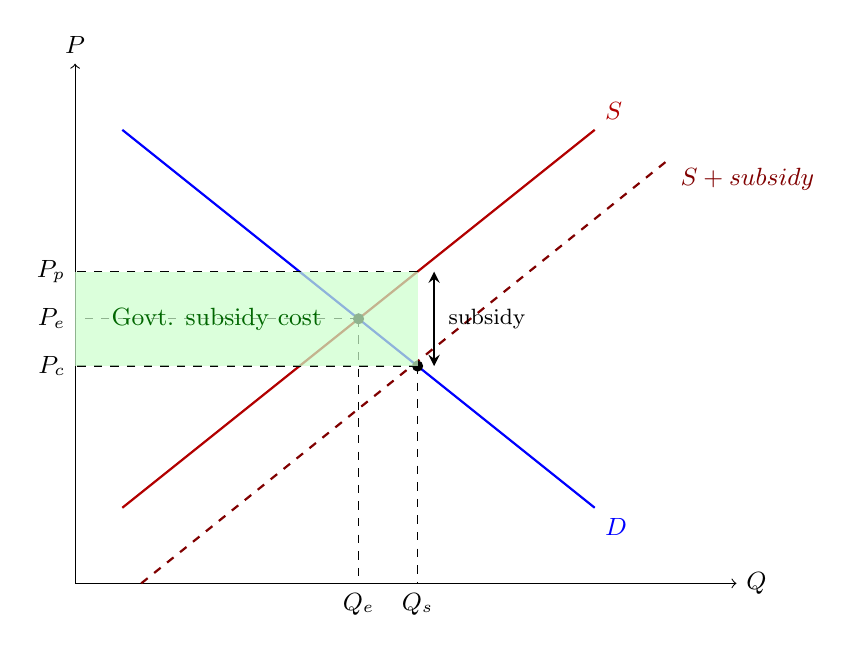
\begin{tikzpicture}[scale=1.2]
\draw[->] (0,0) -- (7,0) node[right, font=\small] {$Q$};
\draw[->] (0,0) -- (0,5.5) node[above, font=\small] {$P$};
% Original supply S
\draw[thick, red!70!black] (0.5,0.8) -- (5.5,4.8) node[above right, red!70!black, font=\small] {$S$};
% New supply S + subsidy (parallel shift downward/rightward)
\draw[thick, red!50!black, dashed] (0.7,0) -- (6.3,4.5) node[below right, red!50!black, font=\small] {$S + subsidy$};
% Demand D
\draw[thick, blue] (0.5,4.8) -- (5.5,0.8) node[below right, blue, font=\small] {$D$};
% Original equilibrium
\filldraw (3.0,2.8) circle (1.5pt);
\draw[dashed] (3.0,2.8) -- (3.0,0) node[below, font=\small] {$Q_e$};
\draw[dashed] (3.0,2.8) -- (0,2.8) node[left, font=\small] {$P_e$};
% New equilibrium (D intersects S+subsidy): shift down by 1
% S+sub: P = -0.2 + 0.8(Q-0.5); D: P = 4.8 - 0.8(Q-0.5)
% -0.2+0.8(Q-0.5) = 4.8-0.8(Q-0.5), 1.6(Q-0.5)=5.0, Q=3.625
\filldraw (3.625,2.3) circle (1.5pt);
\draw[dashed] (3.625,2.3) -- (3.625,0) node[below, font=\small] {$Q_s$};
% Price paid by consumers Pc (lower)
\draw[dashed] (3.625,2.3) -- (0,2.3) node[left, font=\small] {$P_c$};
% Price received by producers Pp (on original S at Q=3.625): P=0.8+0.8(3.125)=3.3
\draw[dashed] (3.625,3.3) -- (0,3.3) node[left, font=\small] {$P_p$};
% Government subsidy cost: rectangle (Pp - Pc) * Qs
\fill[green!20, opacity=0.7] (0,2.3) rectangle (3.625,3.3);
\node[green!40!black, font=\small] at (1.5,2.8) {Govt. subsidy cost};
% Subsidy wedge
\draw[<->, >=stealth, thick] (3.8,2.3) -- (3.8,3.3);
\node[font=\footnotesize, right] at (3.85,2.8) {subsidy};
\end{tikzpicture}
\end{center}
A subsidy shifts the supply curve \textbf{downward} (rightward) from $S$ to $S + subsidy$. The equilibrium quantity \textbf{increases} from $Q_e$ to $Q_s$. Consumers pay a \textbf{lower price} $P_c$; producers receive a \textbf{higher price} $P_p$ (the government pays the difference). The green rectangle $= (P_p - P_c) \times Q_s$ is the total \textbf{cost of the subsidy to the government}. There is an overallocation of resources to the production of the good.
Consequences for various stakeholders:
\begin{itemize}
  \item Consumers: decrease in price, increase in quantity bought
  \item Producers: increase in quantity supplied, increase in revenue (receives $P_p$)
  \item Government: pays $(P_p-P_c)\times Q_s$ to the producer.
  \item Workers: increased employment
  \item Society as a whole:

\begin{center}
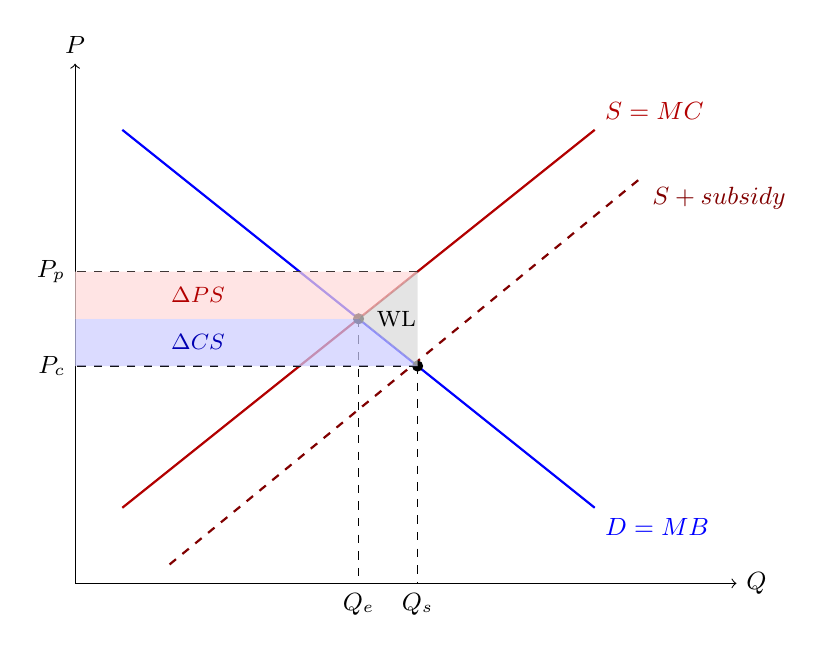
\begin{tikzpicture}[scale=1.2]
\draw[->] (0,0) -- (7,0) node[right, font=\small] {$Q$};
\draw[->] (0,0) -- (0,5.5) node[above, font=\small] {$P$};
% S = MC (original)
\draw[thick, red!70!black] (0.5,0.8) -- (5.5,4.8) node[above right, red!70!black, font=\small] {$S = MC$};
% S + subsidy (shifted down by 1)
\draw[thick, red!50!black, dashed] (1,0.2) -- (6,4.3) node[below right, red!50!black, font=\small] {$S + subsidy$};
% D = MB
\draw[thick, blue] (0.5,4.8) -- (5.5,0.8) node[below right, blue, font=\small] {$D = MB$};
% Original equilibrium
\filldraw (3.0,2.8) circle (1.5pt);
\draw[dashed] (3.0,2.8) -- (3.0,0) node[below, font=\small] {$Q_e$};
% New equilibrium (D intersects S+subsidy): Q=3.625
\filldraw (3.625,2.3) circle (1.5pt);
\draw[dashed] (3.625,2.3) -- (3.625,0) node[below, font=\small] {$Q_s$};
% Pc (price consumers pay)
\draw[dashed] (3.625,2.3) -- (0,2.3) node[left, font=\small] {$P_c$};
% Pp (price producers receive, on original S at Q=3.625)
\draw[dashed] (3.625,3.3) -- (0,3.3) node[left, font=\small] {$P_p$};
% Change in CS: trapezoid between Pe and Pc, under D, from 0 to Qs
\fill[blue!20, opacity=0.7] (0,2.3) -- (0,2.8) -- (3.0,2.8) -- (3.625,2.3) -- cycle;
\node[blue!70!black, font=\footnotesize] at (1.3,2.55) {$\Delta CS$};
% Change in PS: trapezoid between Pe and Pp, above S, from 0 to Qs
\fill[red!15, opacity=0.7] (0,2.8) -- (0,3.3) -- (3.625,3.3) -- (3.0,2.8) -- cycle;
\node[red!70!black, font=\footnotesize] at (1.3,3.05) {$\Delta PS$};
% Welfare loss: triangle between S(MC) and D(MB) from Qe to Qs
\fill[gray!30, opacity=0.7] (3.0,2.8) -- (3.625,2.3) -- (3.625,3.3) -- cycle;
\node[font=\footnotesize] at (3.4,2.8) {WL};
\end{tikzpicture}
\end{center}
The granting of a subsidy results in greater consumer and producer surplus; however, society loses due to government spending on the subsidy. Since the loss from government spending is greater than the gain in consumer and producer surplus, welfare loss results, reflecting allocative inefficiency, which in this case is due to overallocation of resources to the production of the good (overproduction).
\end{itemize}
\subsubsection*{Calculating the effects of subsidies on market outcomes and social welfare}
Change in consumer expenditure: $P_c\times Q_s-P_e\times Q_e$\\
Change in producer revenue: $P_p\times Q_s-P_e\times Q_e$\\
Government expenditure: $(P_p-P_c)\times Q_s$\\
Change in CS: $\dfrac{1}{2}(Q_e+Q_s)\times (P_e-P_c)$\\
Change in PS: $\dfrac{1}{2}(Q_e+Q_s)\times (P_p-P_c)$\\
DWT / welfare loss: $\dfrac{1}{2}(Q_s-Q_e)\times (P_p-P_c)$

\subsection{Supplementary: Government failure (Edexcel Book 1 Ch 20)}
\needbold{Government failure} occurs when government intervention creates a \textbf{worse} outcome than the market failure it was meant to correct (or causes a new inefficiency, leading to a net welfare loss). Causes:
\begin{itemize}
  \item \textbf{Information failure / inadequate information}: governments cannot possess full knowledge of consumer preferences, true costs, or market dynamics, leading to wrong tax/subsidy levels or misallocation.
  \item \textbf{Regulatory capture}: regulatory bodies set up to protect public interest end up serving the commercial interests of the dominant firms they are supposed to regulate.
  \item \textbf{Policy myopia / short-termism}: politicians prioritise short-term electoral cycles over long-run economic efficiency (e.g.\ populist spending or tax cuts).
  \item \textbf{Unintended consequences}: policies frequently produce unanticipated side-effects (e.g.\ rent controls leading to severe housing shortages and black markets; generous unemployment benefits reducing work incentives).
  \item \textbf{Administrative and bureaucratic costs}: the enforcement, monitoring, and compliance costs of intervention may outweigh the social benefits generated.
  \item \textbf{Equity--efficiency trade-offs}: aggressive redistribution policies (high progressive taxes and transfer payments) can distort market price signals and reduce incentives to work and invest.
\end{itemize}
\section{Market failure and socially undesirable outcomes I}
\subsection{The meaning of common pool resources}
\needbold{Common pool resources} are resources that are not owned by anyone, do not have a price and are available for anyone to use without payment or any other restriction.\\\\
Two important concepts:
\begin{itemize}
  \item \needbold{Rivalrous}: its consumption by one person reduces its availability for someone else.
  \item \needbold{Excludable}: it is possible to exclude people from using the good (by charging a price)
\end{itemize}
Common pool resources are rivalrous but non­excludable. 
\subsubsection*{Sustainability and common pool resources}
\textbf{Sustainable resource use} means using a resource at a rate that allows it to regenerate, so its quantity and quality are maintained over time. For biological resources (forests, fish stocks), the key concept is the \textbf{maximum sustainable yield (MSY)} --- the largest quantity that can be harvested indefinitely without depleting the resource.

\begin{center}
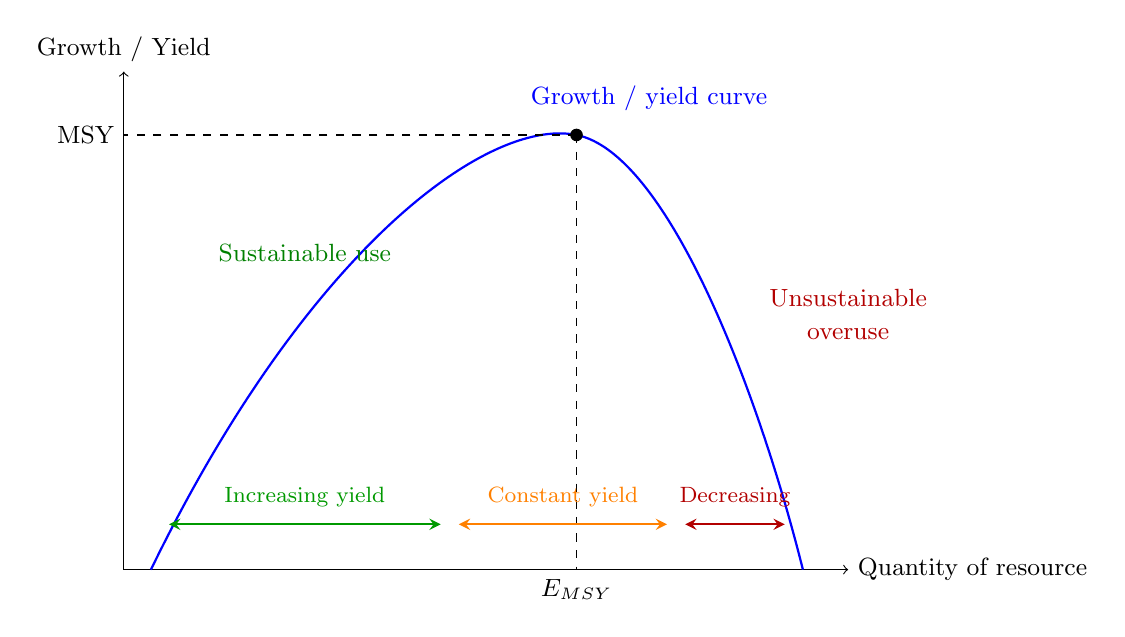
\begin{tikzpicture}[scale=1.15]
\draw[->] (0,0) -- (8,0) node[right, font=\small] {Quantity of resource};
\draw[->] (0,0) -- (0,5.5) node[above, font=\small] {Growth / Yield};
% Growth curve: rises, peaks (MSY), then falls
% S-shaped then inverted: y = a*x*(b-x) type, but let's use a bezier
\draw[thick, blue] (0.3,0) .. controls (2.0,3.5) and (4.0,5.0) .. (5.0,4.8);
\draw[thick, blue] (5.0,4.8) .. controls (6.0,4.6) and (7.0,2.0) .. (7.5,0);
\node[blue, font=\small, right] at (7.5,0) {};
\node[blue, font=\small] at (5.8,5.2) {Growth / yield curve};
% MSY point
\filldraw (5.0,4.8) circle (1.8pt);
\draw[dashed] (5.0,4.8) -- (5.0,0) node[below, font=\small] {$E_{MSY}$};
\draw[dashed] (5.0,4.8) -- (0,4.8) node[left, font=\small] {MSY};
% Phase 1: increasing yield (below MSY, underuse)
\draw[<->, >=stealth, thick, green!60!black] (0.5,0.5) -- (3.5,0.5);
\node[green!60!black, font=\footnotesize] at (2.0,0.8) {Increasing yield};
% Phase 2: maximum sustainable (constant, near peak)
\draw[<->, >=stealth, thick, orange] (3.7,0.5) -- (6.0,0.5);
\node[orange, font=\footnotesize] at (4.85,0.8) {Constant yield};
% Phase 3: decreasing yield (overuse, beyond MSY)
\draw[<->, >=stealth, thick, red!70!black] (6.2,0.5) -- (7.3,0.5);
\node[red!70!black, font=\footnotesize] at (6.75,0.8) {Decreasing};
% Sustainable vs unsustainable labels
\node[green!50!black, font=\small] at (2,3.5) {Sustainable use};
\node[red!70!black, font=\small] at (8.0,3.0) {Unsustainable};
\node[red!70!black, font=\small] at (8.0,2.6) {overuse};
\end{tikzpicture}
\end{center}
\begin{itemize}
  \item \textbf{Increasing yield phase} (low effort): as harvesting effort increases, yield increases. The resource is being used below its regenerative capacity (\textbf{underuse}).
  \item \textbf{Maximum sustainable yield (MSY)}: the peak of the growth curve. Harvesting at $E_{MSY}$ allows the resource to regenerate indefinitely --- this is \textbf{sustainable use}.
  \item \textbf{Decreasing yield phase} (effort beyond $E_{MSY}$): over-harvesting reduces the resource's ability to reproduce, so yield falls even as effort increases. Eventually the resource is depleted (\textbf{unsustainable overuse}).
\end{itemize}
Sustainable resource use means that resources are used at a rate that allows them to reproduce themselves, so that they do not become degraded or depleted.
\subsection{Market failure and externalities}
\needbold{Market failure} refers to the failure of the market to allocate resources efficiently. Market failure results in allocative inefficiency, where too much or too little of goods or services are produced and consumed from the point of view of what is socially most desirable. 
\begin{itemize}
  \item Overprovision of a good means too many resources are allocated to its production (overallocation);
  \item Underprovision means that too few resources are allocated to its production (underallocation).
\end{itemize}
An \needbold{externality} occurs when the actions of consumers or producers give rise to negative or positive side-effects on other people who are not part of these actions, and whose interests are not taken into consideration. 
\begin{itemize}
  \item If the side-effects on third parties involve benefits, there arises a positive externality, also known as external (or spillover) benefit;
  \item If they involve costs, in the form of negative side-effects, there arises a negative externality, also known as external (or spillover) costs. 
\end{itemize} 
Externalities can result either from consumption activities or production activities.
When there are \textbf{no externalities}, private costs/benefits and social costs/benefits coincide:
\begin{itemize}
  \item \textbf{Demand} $= MPB = MSB$ (marginal private benefit $=$ marginal social benefit)
  \item \textbf{Supply} $= MPC = MSC$ (marginal private cost $=$ marginal social cost)
\end{itemize}

\begin{center}
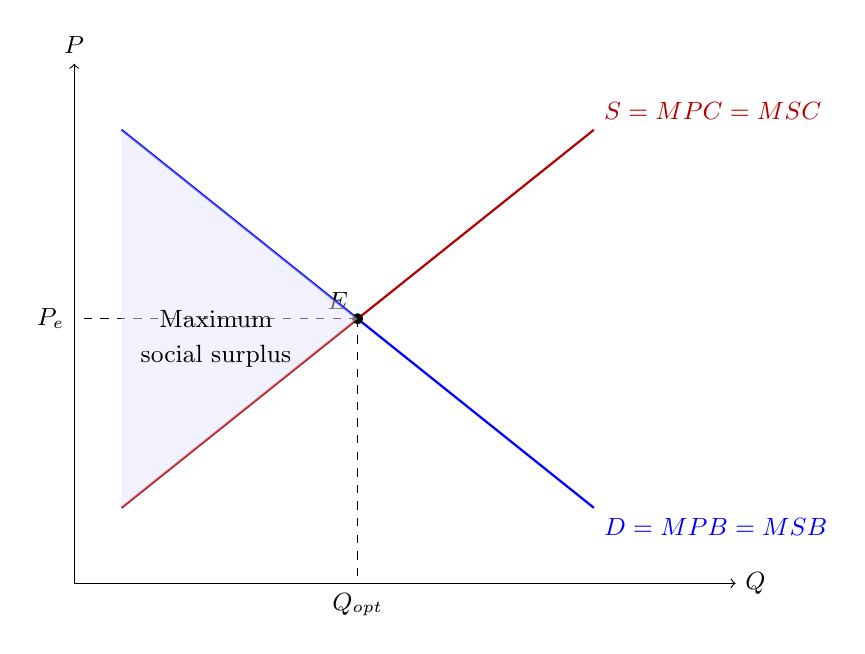
\begin{tikzpicture}[scale=1.2]
\draw[->] (0,0) -- (7,0) node[right, font=\small] {$Q$};
\draw[->] (0,0) -- (0,5.5) node[above, font=\small] {$P$};
% D = MPB = MSB
\draw[thick, blue] (0.5,4.8) -- (5.5,0.8) node[below right, blue, font=\small] {$D = MPB = MSB$};
% S = MPC = MSC
\draw[thick, red!70!black] (0.5,0.8) -- (5.5,4.8) node[above right, red!70!black, font=\small] {$S = MPC = MSC$};
% Equilibrium
\filldraw (3.0,2.8) circle (1.5pt) node[above left, font=\small] {$E$};
\draw[dashed] (3.0,2.8) -- (3.0,0) node[below, font=\small] {$Q_{opt}$};
\draw[dashed] (3.0,2.8) -- (0,2.8) node[left, font=\small] {$P_e$};
% Social surplus region
\fill[blue!10, opacity=0.5] (0.5,4.8) -- (3.0,2.8) -- (0.5,0.8) -- cycle;
\node[font=\small] at (1.5,2.8) {Maximum};
\node[font=\small] at (1.5,2.4) {social surplus};
\end{tikzpicture}
\end{center}
With no externalities, the free-market equilibrium at $Q_{opt}$ achieves \textbf{allocative efficiency}: $MSB = MSC$, social surplus is maximised, and there is no welfare loss. The socially optimal quantity $Q_{opt}$ is identical to the market equilibrium quantity.
\\If, however, there is an externality, additional benefits 
or additional costs affecting third parties arise, and the full benefits or full costs to society differ from the private ones. When this occurs, the equilibrium price and quantity determined by the intersection of the demand (MPB) curve and supply (MPC) curve is no longer a social optimum.
\begin{itemize}
  \item MPC: costs to producers of producing one more unit of a good.
  \item MSC: costs to society of producing one more unit of a good.
  \item MPB: benefits to consumers from consuming one more unit of a good.
  \item MSB: benefits to society from consuming one more unit of a good.
\end{itemize}
\subsection{Negative production externalities}
\textbf{Negative production externalities} occur when production imposes \textbf{external costs} on third parties (e.g.\ pollution from a factory). The social cost of production exceeds the private cost:
\begin{itemize}
  \item $MSC = MPC + MEC$ (marginal external cost)
  \item Since $MEC > 0$, $MSC > MPC$ $\Rightarrow$ the $MSC$ curve lies \textbf{above} the $MPC$ ($S$) curve.
  \item Demand is unaffected: $MPB = MSB$.
\end{itemize}

\begin{center}
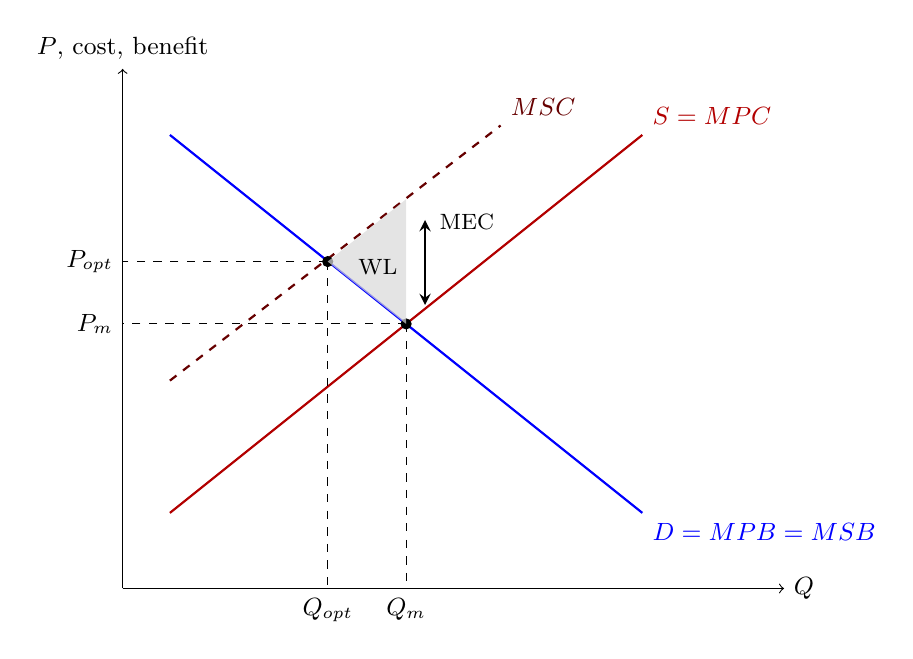
\begin{tikzpicture}[scale=1.2]
\draw[->] (0,0) -- (7,0) node[right, font=\small] {$Q$};
\draw[->] (0,0) -- (0,5.5) node[above, font=\small] {$P$, cost, benefit};
% D = MPB = MSB
\draw[thick, blue] (0.5,4.8) -- (5.5,0.8) node[below right, blue, font=\small] {$D = MPB = MSB$};
% S = MPC
\draw[thick, red!70!black] (0.5,0.8) -- (5.5,4.8) node[above right, red!70!black, font=\small] {$S = MPC$};
% MSC (steeper, above MPC)
\draw[thick, red!40!black, dashed] (0.5,2.2) -- (4.0,4.9) node[above right, red!40!black, font=\small] {$MSC$};
% Market equilibrium (D intersect S=MPC): Q=3.0
\filldraw (3.0,2.8) circle (1.5pt);
\draw[dashed] (3.0,2.8) -- (3.0,0) node[below, font=\small] {$Q_m$};
\draw[dashed] (3.0,2.8) -- (0,2.8) node[left, font=\small] {$P_m$};
% Social optimum (D intersect MSC): solve MSC intersect D
% MSC: P = 1.8 + 3.5/3.5*(Q-0.5) = 1.8 + (Q-0.5) = Q + 1.3; D: P = 4.8 - 0.8*(Q-0.5) = 5.2 - 0.8Q
% Q+1.3 = 5.2-0.8Q, 1.8Q = 3.9, Q = 2.17
\filldraw (2.17,3.46) circle (1.5pt);
\draw[dashed] (2.17,3.46) -- (2.17,0) node[below, font=\small] {$Q_{opt}$};
\draw[dashed] (2.17,3.46) -- (0,3.46) node[left, font=\small] {$P_{opt}$};
% Welfare loss triangle: between Q_opt and Q_m, bounded by MSC above and MSB below
\fill[gray!30, opacity=0.7] (2.17,3.46) -- (3.0,2.8) -- (3.0,4.12) -- cycle;
\node[font=\footnotesize] at (2.7,3.4) {WL};
% MEC bracket
\draw[<->, >=stealth, thick] (3.2,3.0) -- (3.2,3.9);
\node[font=\footnotesize, above right] at (3.25,3.7) {MEC};
\end{tikzpicture}
\end{center}
The \textbf{free market overproduces}: $Q_m > Q_{opt}$, because producers ignore the external costs. The shaded triangle (WL) is the \textbf{welfare loss} --- units between $Q_{opt}$ and $Q_m$ have $MSC > MSB$, meaning society would be better off if they were not produced. The vertical gap between $MSC$ and $MPC$ is the \textbf{marginal external cost (MEC)} per unit.
\[\text{Welfare loss}=\dfrac{1}{2}(Q_\text{m}-Q_\text{opt})\times (MSC-MPC)\]
The welfare loss could also be understood as a change in total social benefits (change in CS and PS)
\subsubsection*{Policies to correct negative production externalities and evaluation}
\begin{itemize}
  \item Market policies
  \begin{itemize}
    \item Indirect taxes / pigouvian taxes: imposing a tax equal to the \textbf{external cost} ($MEC$) per unit, so the $S = MPC$ curve shifts upward to overlap with $MSC$. The new equilibrium is at the intersection of $MSC$ and $D = MPB = MSB$, yielding the \textbf{optimal} quantity $Q_{opt}$ and price $P_{opt}$.

\begin{center}
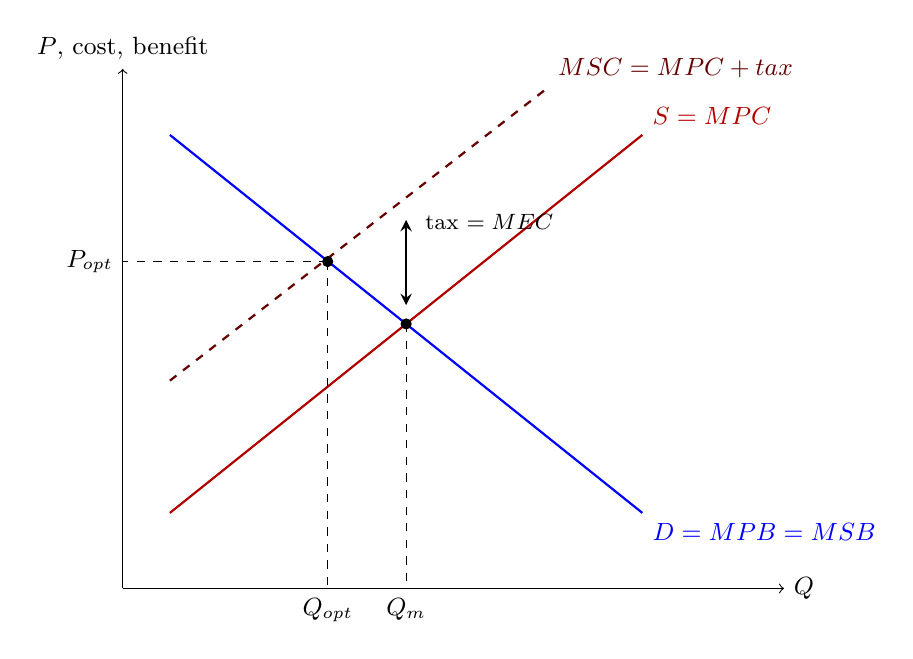
\begin{tikzpicture}[scale=1.2]
\draw[->] (0,0) -- (7,0) node[right, font=\small] {$Q$};
\draw[->] (0,0) -- (0,5.5) node[above, font=\small] {$P$, cost, benefit};
% D = MPB = MSB
\draw[thick, blue] (0.5,4.8) -- (5.5,0.8) node[below right, blue, font=\small] {$D = MPB = MSB$};
% S = MPC (original supply)
\draw[thick, red!70!black] (0.5,0.8) -- (5.5,4.8) node[above right, red!70!black, font=\small] {$S = MPC$};
% MSC (= MPC + tax, parallel shift up)
\draw[thick, red!40!black, dashed] (0.5,2.2) -- (4.5,5.3) node[above right, red!40!black, font=\small] {$MSC = MPC + tax$};
% Market equilibrium (before tax): D intersect S=MPC
\filldraw (3.0,2.8) circle (1.5pt);
\draw[dashed] (3.0,2.8) -- (3.0,0) node[below, font=\small] {$Q_m$};
% Optimal equilibrium (after tax): D intersect MSC
\filldraw (2.17,3.46) circle (1.5pt);
\draw[dashed] (2.17,3.46) -- (2.17,0) node[below, font=\small] {$Q_{opt}$};
\draw[dashed] (2.17,3.46) -- (0,3.46) node[left, font=\small] {$P_{opt}$};
% Tax per unit label
\draw[<->, >=stealth, thick] (3.0,3.0) -- (3.0,3.9);
\node[font=\footnotesize, above right] at (3.1,3.7) {tax $= MEC$};
\end{tikzpicture}
\end{center}
    \item Carbon taxes: tax per unit of carbon emissions of fossil fuels. Following the imposition of the tax, firms must pay the higher price to buy the fossil fuel. The increase in the price of the high-carbon fuel creates incentives for firms to switch to other, less polluting or non-polluting energy sources. If a firm switches to less polluting resources, the external costs of production fall, so the $MSC$ curve shifts \textbf{downward} (from $MSC_1$ to $MSC_2$). With lower external costs, the optimal quantity \textbf{increases} from $Q_{opt,1}$ to $Q_{opt,2}$, and the optimal tax needed (the gap between $MSB$ and $MSC_2$) is smaller.

\begin{center}
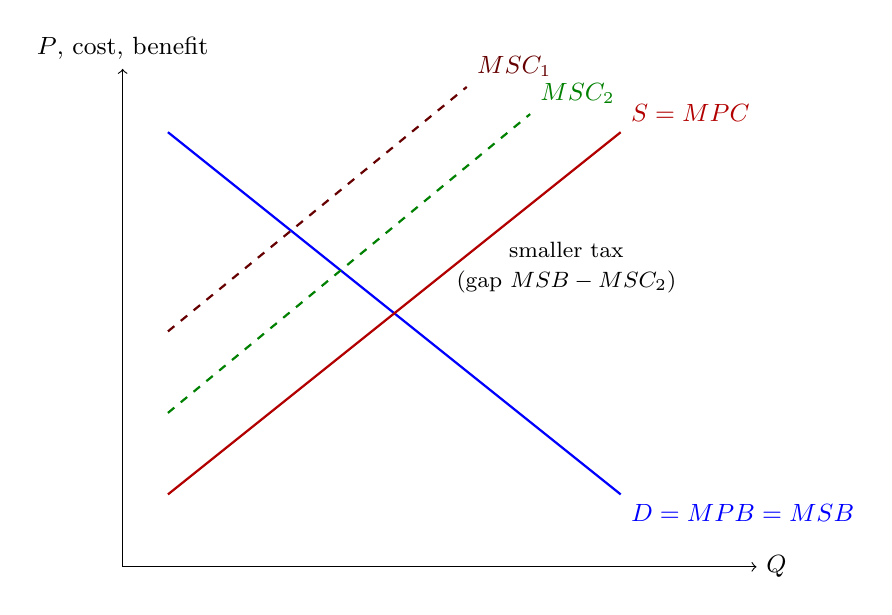
\begin{tikzpicture}[scale=1.15]
\draw[->] (0,0) -- (7,0) node[right, font=\small] {$Q$};
\draw[->] (0,0) -- (0,5.5) node[above, font=\small] {$P$, cost, benefit};
% D = MPB = MSB
\draw[thick, blue] (0.5,4.8) -- (5.5,0.8) node[below right, blue, font=\small] {$D = MPB = MSB$};
% S = MPC
\draw[thick, red!70!black] (0.5,0.8) -- (5.5,4.8) node[above right, red!70!black, font=\small] {$S = MPC$};
% MSC_1 (original, higher external cost)
\draw[thick, red!40!black, dashed] (0.5,2.6) -- (3.8,5.3) node[above right, red!40!black, font=\small] {$MSC_1$};
% MSC_2 (after switching to cleaner resources, lower external cost)
\draw[thick, green!50!black, dashed] (0.5,1.7) -- (4.5,5.0) node[above right, green!50!black, font=\small] {$MSC_2$};
% Smaller tax label
\node[font=\footnotesize] at (4.9,3.5) {smaller tax};
\node[font=\footnotesize] at (4.9,3.15) {(gap $MSB - MSC_2$)};
\end{tikzpicture}
\end{center}
 \item Tradable permits: policy involving permits to pollute issued to firms by a government or an international body. The total pollution allowed must be \textbf{less} than the unregulated level for the scheme to reduce pollution. Permits can be traded between firms.
    \begin{itemize}
      \item The \textbf{supply of permits is perfectly inelastic}, fixed by the government.
      \item The \textbf{demand for permits} determines the equilibrium price.
      \item If a firm can produce with lower emissions than its permits allow, it can \textbf{sell} the extras $\to$ profit.
      \item If a firm needs to emit more than its permits allow, it must \textbf{buy} more $\to$ cost.
      \item As the economy grows and output rises, demand for permits shifts \textbf{rightward} ($D_1 \to D_2$), so the permit price rises ($P_1 \to P_2$).
      \item Like carbon taxes, tradable permits incentivise producers to switch to less polluting resources, reducing the externality and shifting $MSC$ downward toward $MPC$ (as in Figure 5.5(b)).
    \end{itemize}

\begin{center}
\begin{tikzpicture}[scale=1.2]
\draw[->] (0,0) -- (7,0) node[right, font=\small] {Quantity of permits};
\draw[->] (0,0) -- (0,5.5) node[above, font=\small] {Price of permits};
% Vertical supply (fixed)
\draw[thick, red!70!black] (3.0,0.5) -- (3.0,5.0) node[above, red!70!black, font=\small] {$S$ (fixed)};
% Demand curve D1
\draw[thick, blue] (0.5,4.5) -- (5.5,1.0) node[below right, blue, font=\small] {$D_1$};
% Demand curve D2 (shifted right)
\draw[thick, blue!60!green, dashed] (1.5,4.6) -- (5.5,1.8) node[below right, blue!60!green, font=\small] {$D_2$};
% Equilibrium 1 (S intersect D1)
\filldraw (3.0,2.78) circle (1.5pt);
\draw[dashed] (3.0,2.78) -- (0,2.78) node[left, font=\small] {$P_1$};
% Equilibrium 2 (S intersect D2)
\filldraw (3.0,3.6) circle (1.5pt);
\draw[dashed] (3.0,3.6) -- (0,3.6) node[left, font=\small] {$P_2$};
% Fixed quantity label
\draw[dashed] (3.0,0.5) -- (3.0,0) node[below, font=\small] {$Q_{permits}$};
\end{tikzpicture}
\end{center}
  \end{itemize}
  \begin{itemize}
    \item \textbf{Pros (advantages of market-based policies):}
    \begin{itemize}
      \item \textbf{Internalise the externality}: external costs become paid for by producers/consumers, aligning private with social costs.
      \item \textbf{Taxes on pollutants $>$ taxes on output}: emission taxes (e.g.\ carbon taxes) incentivise firms to \textit{economise on polluting inputs} and switch to cleaner technology, whereas output taxes only reduce quantity produced with the same dirty technology.
      \item \textbf{Least-cost pollution reduction}: firms facing lower clean-up costs cut pollution first; high-cost firms pay the tax or buy permits $\to$ society achieves a given emission cut at the \textit{lowest overall cost}.
      \item \textbf{Tradable permits} similarly reward low-cost abaters (they sell excess permits) and penalise high-cost ones (they must buy).
      \item \textbf{Government revenue}: taxes generate revenue that can be used for related spending (e.g.\ clean energy investment).
    \end{itemize}
    \item \textbf{Cons (disadvantages of market-based policies):}
    \begin{itemize}
      \item \textbf{Technical difficulty of measuring harm}: enormous uncertainty over which production methods/pollutants cause what damage, and how to attach a monetary value to the harm.
      \item \textbf{Taxes}: must equal $MEC$ per unit, which is unknown. 
      \begin{itemize}
        \item What production methods produce pollutants?
        \item Which pollutants are harmful?
        \item What is the value of the harm?
        \item What is the appropriate amount of tax? 
        \item How will consumers be affected? 
      \end{itemize}
      In practice, carbon taxes are usually set \textit{too low} for political reasons, limiting their impact.
      \item \textbf{Indirect taxes are regressive}: lower-income households pay a higher proportion of their income in tax than higher-income households $\to$ \textbf{inequitable}.
      \item \textbf{Firms may keep polluting}: even if they pay the tax, some firms do not reduce emissions.
      \item \textbf{Tradable permits:} setting the maximum acceptable pollution level requires technical info often unavailable. Too high $\to$ ineffective; too low $\to$ permits become very costly for firms. This results in permits developed for only a few types of pollutants. 
      \item \textbf{Distribution of permits} may involve political favouritism.
      \item In practice, the best achievable outcome is usually only a partial shift of $MPC$ toward $MSC$ and some reduction in the externality; full optimality is unlikely.
    \end{itemize}
  \end{itemize}
  \item Government legislation and regulation: intended to reduce the effects of production externalities and limit environmental damage typically involve emissions standards, quotas, licences, permits or outright restrictions. Examples: 
  \begin{itemize}
    \item restrictions on emissions of pollutants from
factories and industrial production by setting a maximum level of pollutants permitted
\item requirements for steel mills and electricity
generating plants to install smokestack scrubbers to reduce emissions
\item banning the use of harmful substances (e.g.
asbestos, a group of minerals that are very toxic that is banned in many countries)
\item issuing licences or permits for particular activities (such as hunting)
\item prohibiting construction (such as housing) or industry or agriculture in protected areas
\item restrictions on the quantity of logging
\item restrictions in the form of quotas for fishing (maximum permissible quantity of fish that can be caught) or in the form of the size of shipping fleets, or total bans for specific areas or specific times of the year
\item establishment of protected areas for the protection of biodiversity and endangered ecosystems.
  \end{itemize}
  This results in shifting the MPC curve upward towards the MSC curve.
  \begin{itemize}
    \item \textbf{Pros:}
    \begin{itemize}
      \item \textbf{Simple to implement and oversee}; avoid the technical difficulties of market-based policies.
      \item \textbf{Can be very effective}: banning harmful substances, prohibiting hunting in certain areas, or restricting logging may be the \textit{most effective} way to deal with certain problems.
      \item \textbf{Force compliance}: firms must reduce harmful activities (market-based policies may not always achieve this).
      \item \textbf{Most widely used} method to limit negative externalities worldwide.
    \end{itemize}
    \item \textbf{Cons:}
    \begin{itemize}
      \item \textbf{No incentive} to reduce emissions via cleaner resources, energy efficiency, or alternative fuels --- firms only comply with the set standard.
      \item \textbf{Cannot distinguish between firms} with low vs.\ high pollution-reduction costs $\to$ pollution is reduced at a \textit{higher overall cost} than market-based policies.
      \item \textbf{Same technical limitations} as market-based policies (lack of information on pollutant types and quantities) $\to$ only \textit{partially effective}.
      \item \textbf{Costly monitoring and supervision} to detect violations; OPC and enforcement problems.
      \item Effectiveness varies with the situation --- more effective in some contexts than others.
    \end{itemize}
  \end{itemize}
  \item \textbf{Collective self-governance}: a solution where \textbf{users themselves} take control of common pool resources and manage them sustainably --- countering the \textbf{tragedy of the commons}, where each user exploits the resource at the expense of others until it is degraded/depleted.
  \begin{itemize}
    \item \textbf{Pros:}
    \begin{itemize}
      \item Demonstrates people can solve overuse problems \textbf{cooperatively}, without govt. intervention or private ownership.
      \item Works in the absence of both private property (free-market solution) and government property (command-economy solution).
      \item Communities craft \textbf{locally-tailored rules and enforcement mechanisms} that fit their specific resource setting.
      \item Requires only that users can \textbf{communicate} and that the resource has \textbf{clear boundaries}.
    \end{itemize}
    \item \textbf{Cons:}
    \begin{itemize}
      \item Requires \textbf{effective communication} among users to create and agree on rules --- fails if communication is poor or self-organisation costs are too high.
      \item Requires \textbf{well-defined boundaries} for the resource (e.g.\ a pasture, lake, or wood).
      \item \textbf{Ill-suited to global resources} such as the oceans or the global climate, where boundaries are hard to define and users cannot easily communicate or enforce rules (Ostrom herself despaired over the oceans).
      \item Requires a supporting \textbf{legal system of land/resource rights} to function effectively.
    \end{itemize}
  \end{itemize}
  \item \textbf{Education and awareness creation}: educating the public and providing information about firms' polluting activities can lead consumers to \textbf{turn away} from offending firms' products, forcing firms to change their production methods.
  \begin{itemize}
    \item \textbf{Pros}: firms are strongly influenced by customer opinions and want to avoid drops in sales.
    \item \textbf{Cons}: only makes a \textbf{small difference}; effective for localised, high-profile issues (e.g.\ an oil spill) where consumers may boycott, but broad problems like fossil-fuel-driven climate change require solutions on a far larger scale (carbon taxes, tradable permits are far more effective).
  \end{itemize}
  \item \textbf{International agreements}: negative production externalities and overuse of common pool resources often have \textbf{international repercussions}, requiring \textbf{cooperation among govts}. Co-operation may be \textit{global} or \textit{regional}, and is also crucial for the development and diffusion of new green technologies.\\
  \textbf{Key challenge}: global common pool resources (oceans, climate, ozone) are owned by no one, so no single country can claim damages for their destruction --- responsibility is diffuse and consequences are felt worldwide, making enforcement difficult.
\end{itemize}
\subsection{Negative consumption externalities}
\textbf{Negative consumption externalities} occur when consumption imposes \textbf{external costs} on third parties (e.g.\ second-hand smoke, litter). The social benefit of consumption is less than the private benefit:
\begin{itemize}
  \item $MSB = MPB - MEB$ (marginal external benefit is negative; i.e.\ there is a marginal external cost)
  \item Since there is an external cost, $MSB < MPB$ $\Rightarrow$ the $MSB$ curve lies \textbf{below} the $MPB$ ($D$) curve.
  \item Supply is unaffected: $MPC = MSC$.
\end{itemize}

\begin{center}
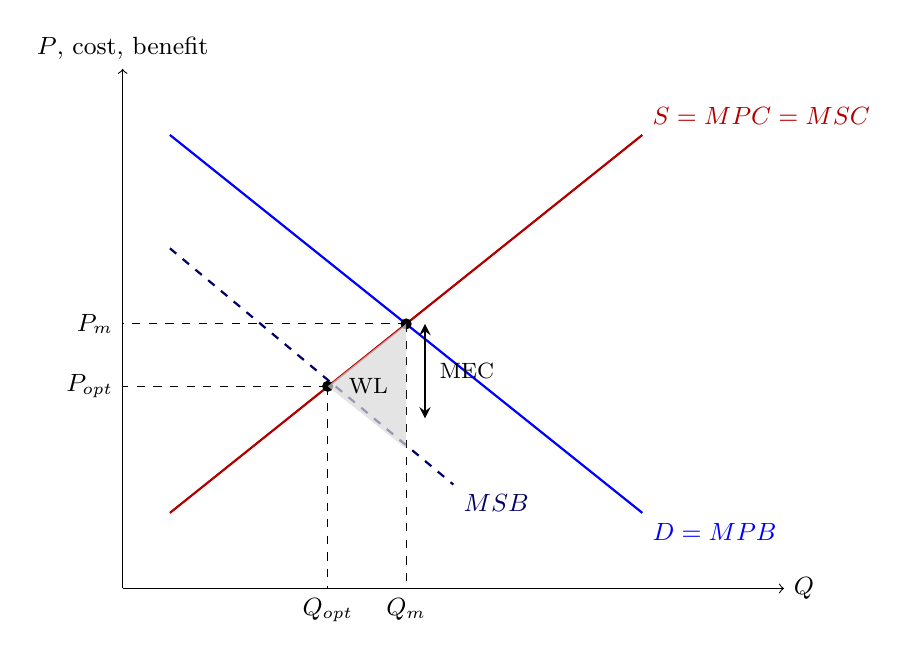
\begin{tikzpicture}[scale=1.2]
\draw[->] (0,0) -- (7,0) node[right, font=\small] {$Q$};
\draw[->] (0,0) -- (0,5.5) node[above, font=\small] {$P$, cost, benefit};
% S = MPC = MSC
\draw[thick, red!70!black] (0.5,0.8) -- (5.5,4.8) node[above right, red!70!black, font=\small] {$S = MPC = MSC$};
% D = MPB
\draw[thick, blue] (0.5,4.8) -- (5.5,0.8) node[below right, blue, font=\small] {$D = MPB$};
% MSB (below MPB, steeper downward)
\draw[thick, blue!40!black, dashed] (0.5,3.6) -- (3.5,1.1) node[below right, blue!40!black, font=\small] {$MSB$};
% Market equilibrium (D intersect S): Q=3.0
\filldraw (3.0,2.8) circle (1.5pt);
\draw[dashed] (3.0,2.8) -- (3.0,0) node[below, font=\small] {$Q_m$};
\draw[dashed] (3.0,2.8) -- (0,2.8) node[left, font=\small] {$P_m$};
% Social optimum (MSB intersect S=MSC): MSB: P=3.8-3/3*(Q-0.5)=3.8-(Q-0.5)=4.3-Q; S: P=0.8+0.8(Q-0.5)=0.4+0.8Q
% 4.3-Q = 0.4+0.8Q, 3.9=1.8Q, Q=2.17
\filldraw (2.17,2.14) circle (1.5pt);
\draw[dashed] (2.17,2.14) -- (2.17,0) node[below, font=\small] {$Q_{opt}$};
\draw[dashed] (2.17,2.14) -- (0,2.14) node[left, font=\small] {$P_{opt}$};
% Welfare loss triangle: between Q_opt and Q_m, bounded by MSC above and MSB below
\fill[gray!30, opacity=0.7] (2.17,2.14) -- (3.0,2.8) -- (3.0,1.48) -- cycle;
\node[font=\footnotesize] at (2.6,2.14) {WL};
% MEC bracket
\draw[<->, >=stealth, thick] (3.2,1.8) -- (3.2,2.8);
\node[font=\footnotesize, right] at (3.25,2.3) {MEC};
\end{tikzpicture}
\end{center}
The \textbf{free market overconsumes}: $Q_m > Q_{opt}$, because consumers ignore the external costs of their consumption. The shaded triangle (WL) is the \textbf{welfare loss} --- units between $Q_{opt}$ and $Q_m$ have $MSC > MSB$, meaning society would be better off if they were not consumed. The vertical gap between $MPB$ and $MSB$ is the \textbf{marginal external cost (MEC)} per unit.\\
Welfare loss can be calculated as
\[\text{Welfare loss}=\dfrac{1}{2}(Q_m-Q_{opt})\times (MPB-MSB)\]
It could also be thought as total social surplus (CS+PS) - total social benefits (CS+PS-external cost)
\subsubsection*{Demerit goods and overuse of CPR}
\needbold{Demerit goods} are goods that are considered to be undesirable for consumers, but which are overprovided by the market. One common reason that they are overprovided is because of negative consumption externalities. Overuse of common pool resources is seen as resulting more from production activities than consumption activities, therefore relating more to negative production rather than consumption externalities. However, overuse of common pool resources also results from negative consumption externalities.
\subsubsection*{Policies to correct NCE and prevent overuse of CPR}
\begin{itemize}
  \item Market-based
  \begin{itemize}
    \item \textbf{Indirect (Pigouvian) taxes}: imposed on goods whose consumption creates external costs (e.g.\ cigarettes, petrol/gasoline). The tax shifts the supply curve \textbf{upward} from $S = MPC$ to $MPC + tax$. If the tax equals the external cost per unit, the $MPC + tax$ curve intersects $D = MPB$ at the socially optimal quantity $Q_{opt}$, where allocative efficiency is achieved. The quantity consumed falls from $Q_m$ to $Q_{opt}$, and the price rises from $P_m$ to $P_c$. (Note: the demand curve does \textit{not} shift.)

\begin{center}
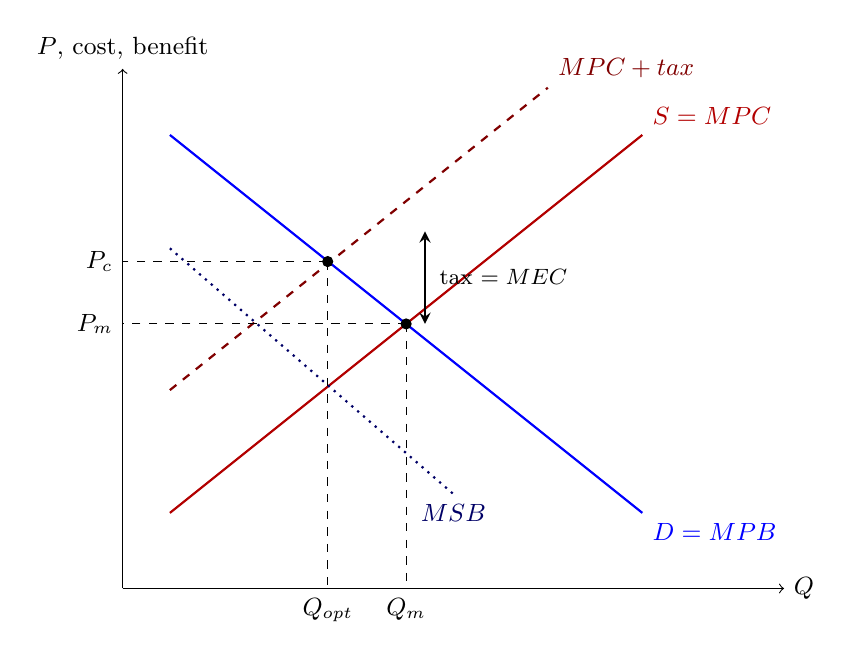
\begin{tikzpicture}[scale=1.2]
\draw[->] (0,0) -- (7,0) node[right, font=\small] {$Q$};
\draw[->] (0,0) -- (0,5.5) node[above, font=\small] {$P$, cost, benefit};
% S = MPC (original supply)
\draw[thick, red!70!black] (0.5,0.8) -- (5.5,4.8) node[above right, red!70!black, font=\small] {$S = MPC$};
% MPC + tax (shifted up to coincide with MSC level)
\draw[thick, red!50!black, dashed] (0.5,2.1) -- (4.5,5.3) node[above right, red!50!black, font=\small] {$MPC + tax$};
% D = MPB
\draw[thick, blue] (0.5,4.8) -- (5.5,0.8) node[below right, blue, font=\small] {$D = MPB$};
% MSB (below MPB)
\draw[thick, blue!40!black, dotted] (0.5,3.6) -- (3.5,1.0) node[below, blue!40!black, font=\small] {$MSB$};
% Market equilibrium (D intersect S=MPC): Q=3.0
\filldraw (3.0,2.8) circle (1.5pt);
\draw[dashed] (3.0,2.8) -- (3.0,0) node[below, font=\small] {$Q_m$};
\draw[dashed] (3.0,2.8) -- (0,2.8) node[left, font=\small] {$P_m$};
% Optimal equilibrium (D=MPB intersect MPC+tax): Q=2.17
\filldraw (2.17,3.46) circle (1.5pt);
\draw[dashed] (2.17,3.46) -- (2.17,0) node[below, font=\small] {$Q_{opt}$};
\draw[dashed] (2.17,3.46) -- (0,3.46) node[left, font=\small] {$P_c$};
% Tax per unit
\draw[<->, >=stealth, thick] (3.2,2.8) -- (3.2,3.78);
\node[font=\footnotesize, right] at (3.25,3.3) {tax $= MEC$};
\end{tikzpicture}
\end{center}
  \end{itemize}
  \begin{itemize}
    \item \textbf{Pros of indirect taxes (market-based policy):}
    \begin{itemize}
      \item \textbf{Internalise the externality}: external costs become paid for by consumers, aligning private with social costs.
      \item \textbf{Change relative prices}: the taxed good becomes relatively more expensive $\to$ consumers reduce consumption.
      \item \textbf{Preferred by economists} over regulation, as long as the situation permits market-based policy.
      \item \textbf{Generate government revenue.}
    \end{itemize}
    \item \textbf{Cons of indirect taxes:}
    \begin{itemize}
      \item \textbf{Difficult to measure external costs}: hard to assess who/what is affected and assign a monetary value (e.g.\ passive smoking, environmental pollution from petrol).
      \item \textbf{Inelastic demand problem}: goods like petrol and cigarettes have \textit{inelastic demand}, so a tax increases price but only slightly reduces quantity demanded $\to$ may mainly raise government revenue without significantly cutting consumption.
      \item Achieving $Q_{opt}$ may require a \textbf{very high tax}, which is often \textbf{politically unacceptable}.
    \end{itemize}
  \end{itemize}
  \subsubsection*{Tax on producers or consumers?}
  It may seem odd that a tax to correct a \textbf{negative consumption} externality is imposed on \textit{producers} (shifting the MPC curve upward) rather than on the consumers who actually create the externality. In fact, the two approaches produce \textbf{identical market outcomes}:
  \begin{itemize}
    \item \textbf{Tax on producers}: the $S = MPC$ curve shifts \textit{upward} to $MPC + tax$. At the new equilibrium, $Q_{opt}$ is produced; consumers pay $P_c$ and producers receive $P_p$.
    \item \textbf{Tax on consumers}: the $D = MPB$ curve shifts \textit{downward} by the amount of the tax. The new equilibrium again yields $Q_{opt}$, with the same $P_c$ (price consumers pay) and $P_p$ (price producers receive).
  \end{itemize}
  Whether the tax is levied on producers or consumers, the resulting $Q_{opt}$, $P_c$ and $P_p$ are the same. The \textbf{distribution of the tax burden} (incidence) between consumers and producers depends only on the \textbf{price elasticities} of demand and supply, not on whom the tax is formally imposed upon.
  \item Government legislation and regulation: If negative consumption externalities were corrected, $Q_{opt}$ quantity of the good would be produced, reflecting allocative efficiency. Regulations can be used to prevent or limit consumer activities that impose costs on third parties. This has the effect of shifting the $D = MPB$ curve towards the $MSB$ curve (until they overlap).
  \begin{itemize}
    \item \textbf{Pros}: can be \textbf{very effective} for certain activities --- e.g.\ prohibiting smoking in public places, restricting cars entering city centres.
    \item \textbf{Cons}: \textbf{cannot be used} for other negative consumption externalities --- e.g.\ it would be very difficult to regulate petrol/gasoline consumption directly. In such cases indirect taxes are more effective (though subject to inelastic demand limitations).
  \end{itemize}
  \item \textbf{Education and awareness creation}: government campaigns to persuade consumers to buy fewer goods with negative externalities (e.g.\ anti-smoking campaigns, unhealthy food warnings, encouraging public transport / home insulation / information on carbon from air travel). The objective is to \textbf{decrease demand} so that $MPB$ shifts leftward to coincide with $MSB$, achieving $Q_{opt}$ at lower price $P_{opt}$.
  \begin{itemize}
    \item \textbf{Pros}: \textbf{simpler} than other methods (taxes, regulation).
    \item \textbf{Cons}: campaigns are funded by \textbf{tax revenue} $\to$ \textbf{opportunity cost} (less funds for elsewhere); may \textbf{not be effective enough} to significantly reduce the externality.
  \end{itemize}
  \item \textbf{Nudges}: behavioural economics methods to influence consumer behaviour --- e.g.\ placing unhealthy foods in less accessible positions in shops, graphic pictures on cigarette packs, creating bicycle lanes to encourage cycling over driving. Like education, nudges aim to \textbf{shift $MPB$ toward $MSB$}; they can also encourage \textit{desirable} behaviour directly.
  \begin{itemize}
    \item \textbf{Cons}: nudges are still a \textbf{new method}; not enough is known about how consumers respond to particular nudges and choice architecture. Effects may \textbf{differ across income and cultural groups}, limiting generalizability.
  \end{itemize}
\end{itemize}
\section{Market failure and socially undesirable outcomes II}
\subsection{Positive production externalities}
\textbf{Positive production externalities} occur when production creates \textbf{external benefits} for third parties (e.g.\ R\&D leading to new technologies, vaccination production). The social cost of production is less than the private cost:
\begin{itemize}
  \item $MSC = MPC - MEB$ (marginal external benefit treated as a ``negative cost'')
  \item Since $MEB > 0$, $MSC < MPC$ $\Rightarrow$ the $MSC$ curve lies \textbf{below} the $MPC$ ($S$) curve.
  \item Demand is unaffected: $MPB = MSB$.
\end{itemize}

\begin{center}
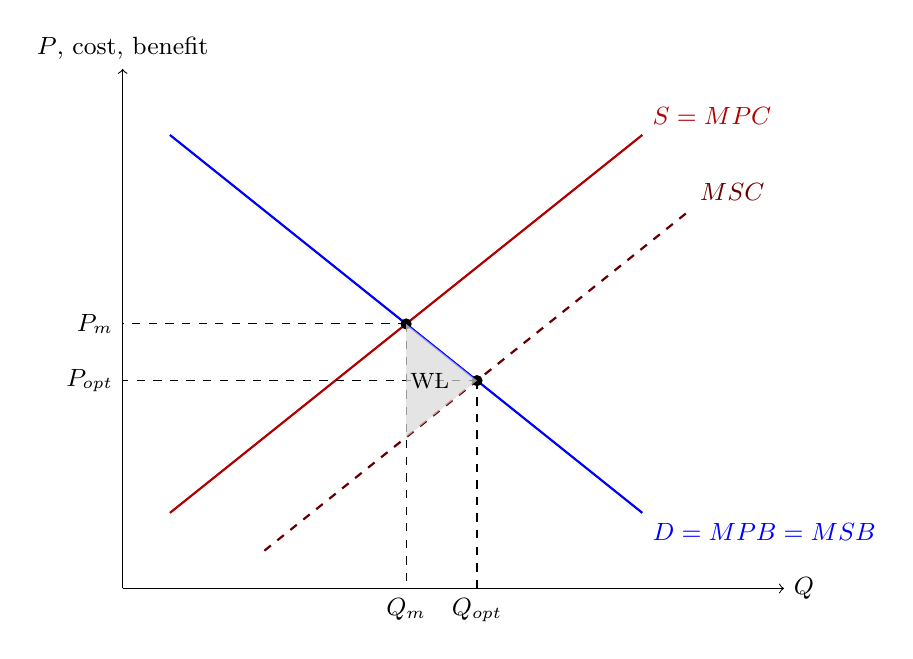
\begin{tikzpicture}[scale=1.2]
\draw[->] (0,0) -- (7,0) node[right, font=\small] {$Q$};
\draw[->] (0,0) -- (0,5.5) node[above, font=\small] {$P$, cost, benefit};
% D = MPB = MSB
\draw[thick, blue] (0.5,4.8) -- (5.5,0.8) node[below right, blue, font=\small] {$D = MPB = MSB$};
% S = MPC
\draw[thick, red!70!black] (0.5,0.8) -- (5.5,4.8) node[above right, red!70!black, font=\small] {$S = MPC$};
% MSC (well below MPC, shallower slope for clear separation)
% MSC through (0.5,-0.5) and (5.0,3.5): slope=4/4.5=0.889... keep parallel but shifted down by ~1.3
% Actually simplest: shift MPC down by 1.2 units -> MSC: P = (0.8-1.2) + 0.8(Q-0.5) = -0.8+0.8Q
% MSC through (0.5,-0.4) and (5.0,3.2)
\draw[thick, red!40!black, dashed] (1.5,0.4) -- (6.0,4.0) node[above right, red!40!black, font=\small] {$MSC$};
% Market equilibrium (D intersect S=MPC): Q=3.0
\filldraw (3.0,2.8) circle (1.5pt);
\draw[dashed] (3.0,2.8) -- (3.0,0) node[below, font=\small] {$Q_m$};
\draw[dashed] (3.0,2.8) -- (0,2.8) node[left, font=\small] {$P_m$};
% Social optimum (D=MSB intersect MSC): MSC: P=-0.4+0.8(Q-0.5)=-0.8+0.8Q
% D: 5.2-0.8Q = -0.8+0.8Q, 6.0=1.6Q, Q=3.75
\filldraw (3.75,2.2) circle (1.5pt);
\draw[dashed] (3.75,2.2) -- (3.75,0) node[below, font=\small] {$Q_{opt}$};
\draw[dashed] (3.75,2.2) -- (0,2.2) node[left, font=\small] {$P_{opt}$};
% Welfare loss triangle: between Q_m and Q_opt, bounded by MPC above and MSB below
\fill[gray!30, opacity=0.7] (3.0,2.8) -- (3.75,2.2) -- (3.0,1.6) -- cycle;
\node[font=\footnotesize] at (3.25,2.2) {WL};
\end{tikzpicture}
\end{center}
The \textbf{free market underproduces}: $Q_m < Q_{opt}$, because producers ignore the external benefits of their production. At $Q_m$, $MSB > MSC$, meaning society would benefit from producing more. The shaded triangle (WL) is the \textbf{welfare loss} --- units between $Q_m$ and $Q_{opt}$ where $MSB > MSC$ are not produced. The vertical gap between $MPC$ and $MSC$ is the \textbf{marginal external benefit (MEB)} per unit.
\\\\Welfare loss can be calculated as
\[\text{Welfare loss}=\dfrac{1}{2}(Q_{opt}-Q_m)\times (MPC-MSC)\]
It can also be interpreted by comparing total social benefits at market equilibrium and social optimum.
\subsubsection*{Correcting positive production externalities}
\begin{itemize}
  \item \textbf{Direct government provision}: the government itself provides the good/service creating the positive externality (e.g.\ R\&D for new technology, medicine/pharmaceuticals, worker training), funded by tax revenue. This shifts the $S = MPC$ curve \textbf{downward (rightward)} toward the $MSC$ curve, increasing quantity to $Q_{opt}$ and lowering price from $P_m$ to $P_{opt}$.
  \item \textbf{Subsidies}: the government grants a per-unit subsidy to producers equal to the \textbf{external benefit} ($MEB$). This shifts the $MPC$ curve \textbf{downward (rightward)} until it coincides with $MSC$, increasing output to $Q_{opt}$ and lowering price to $P_{opt}$. Allocative efficiency is achieved.
\end{itemize}
\begin{center}
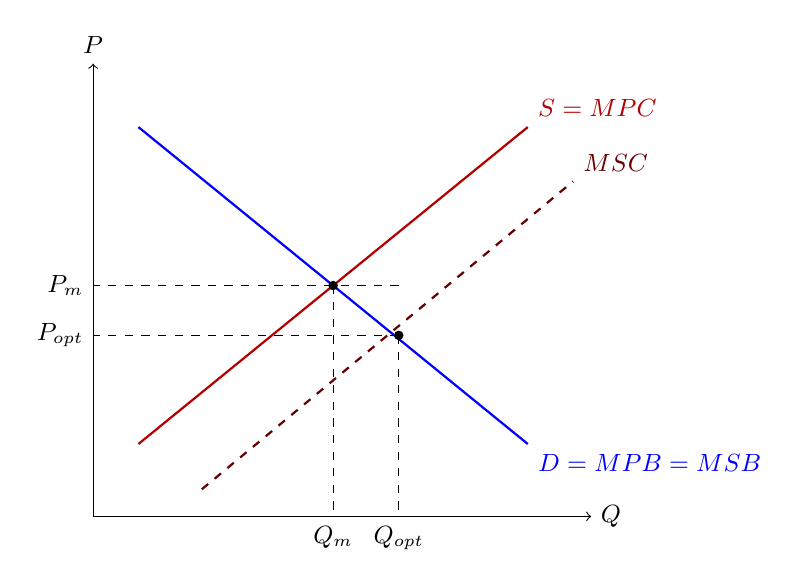
\begin{tikzpicture}[scale=1.15]
% --- (a) Direct government provision ---
\begin{scope}
\draw[->] (0,0) -- (5.5,0) node[right, font=\small] {$Q$};
\draw[->] (0,0) -- (0,5) node[above, font=\small] {$P$};
% D = MPB = MSB
\draw[thick, blue] (0.5,4.3) -- (4.8,0.8) node[below right, blue, font=\small] {$D = MPB = MSB$};
% S = MPC (original)
\draw[thick, red!70!black] (0.5,0.8) -- (4.8,4.3) node[above right, red!70!black, font=\small] {$S = MPC$};
% MSC (below MPC)
\draw[thick, red!40!black, dashed] (1.2,0.3) -- (5.3,3.7) node[above right, red!40!black, font=\small] {$MSC$};
% Market eq
\filldraw (2.65,2.55) circle (1.3pt);
\draw[dashed] (2.65,2.55) -- (2.65,0) node[below, font=\small] {$Q_m$};
% Optimal eq (D intersect MSC): MSC: P=-0.3+0.8(Q-0.5)=-0.7+0.8Q; D: 4.3-0.8(Q-0.5)=4.7-0.8Q
% -0.7+0.8Q = 4.7-0.8Q, 1.6Q=5.4, Q=3.375
\filldraw (3.375,2.0) circle (1.3pt);
\draw[dashed] (3.375,2.0) -- (3.375,0) node[below, font=\small] {$Q_{opt}$};
\draw[dashed] (3.375,2.0) -- (0,2.0) node[left, font=\small] {$P_{opt}$};
\draw[dashed] (3.375,2.55) -- (0,2.55) node[left, font=\small] {$P_m$};
\end{scope}
\end{tikzpicture}
\end{center}
\subsection{Positive consumption externalities}
\textbf{Positive consumption externalities} occur when consumption creates \textbf{external benefits} for third parties (e.g.\ vaccination, education). The social benefit of consumption exceeds the private benefit:
\begin{itemize}
  \item $MSB = MPB + MEB$ (marginal external benefit)
  \item Since $MEB > 0$, $MSB > MPB$ $\Rightarrow$ the $MSB$ curve lies \textbf{above} the $MPB$ ($D$) curve.
  \item Supply is unaffected: $MPC = MSC$.
\end{itemize}

\begin{center}
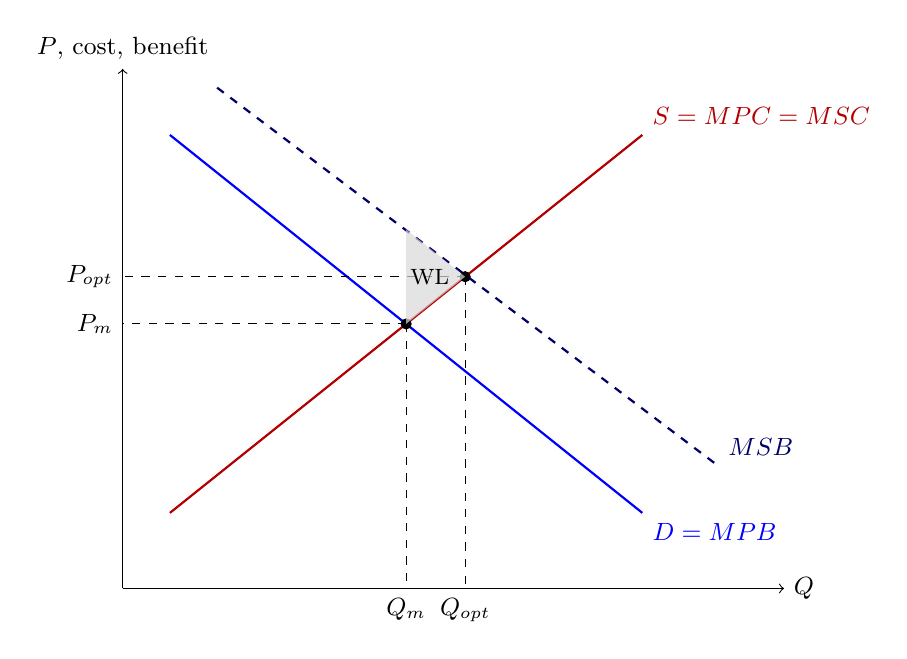
\begin{tikzpicture}[scale=1.2]
\draw[->] (0,0) -- (7,0) node[right, font=\small] {$Q$};
\draw[->] (0,0) -- (0,5.5) node[above, font=\small] {$P$, cost, benefit};
% S = MPC = MSC
\draw[thick, red!70!black] (0.5,0.8) -- (5.5,4.8) node[above right, red!70!black, font=\small] {$S = MPC = MSC$};
% D = MPB
\draw[thick, blue] (0.5,4.8) -- (5.5,0.8) node[below right, blue, font=\small] {$D = MPB$};
% MSB (above MPB, parallel shift up by 1.2)
\draw[thick, blue!40!black, dashed] (1.0,5.3) -- (6.3,1.3) node[above right, blue!40!black, font=\small] {$MSB$};
% Market equilibrium (D=MPB intersect S=MPC): Q=3.0
\filldraw (3.0,2.8) circle (1.5pt);
\draw[dashed] (3.0,2.8) -- (3.0,0) node[below, font=\small] {$Q_m$};
\draw[dashed] (3.0,2.8) -- (0,2.8) node[left, font=\small] {$P_m$};
% Social optimum (MSB intersect S=MSC): MSB: P=5.8-0.8(Q-0.5)=6.2-0.8Q; S: P=0.8+0.8(Q-0.5)=0.4+0.8Q
% 6.2-0.8Q = 0.4+0.8Q, 1.6Q=5.8, Q=3.625
\filldraw (3.625,3.3) circle (1.5pt);
\draw[dashed] (3.625,3.3) -- (3.625,0) node[below, font=\small] {$Q_{opt}$};
\draw[dashed] (3.625,3.3) -- (0,3.3) node[left, font=\small] {$P_{opt}$};
% Welfare loss triangle: between Q_m and Q_opt, bounded by MSB above and MSC below
\fill[gray!30, opacity=0.7] (3.0,2.8) -- (3.625,3.3) -- (3.0,3.8) -- cycle;
\node[font=\footnotesize] at (3.25,3.3) {WL};
\end{tikzpicture}
\end{center}
The \textbf{free market underconsumes}: $Q_m < Q_{opt}$, because consumers ignore the external benefits of their consumption. At $Q_m$, $MSB > MSC$, meaning society would benefit from consuming more. The shaded triangle (WL) is the \textbf{welfare loss} --- units between $Q_m$ and $Q_{opt}$ where $MSB > MSC$ are not consumed. The vertical gap between $MPB$ and $MSB$ is the \textbf{marginal external benefit (MEB)} per unit.\\\\
Welfare loss can be calculated as 
\[\text{Welfare loss}=\dfrac{1}{2}(Q_{opt}-Q_m)\times (MSB-MPB)\]
It could also be interpreted as the difference between social benefits at social optimum - market equilibrium. (CS+PS)
\subsubsection*{Merit goods}
\needbold{Merit goods} are goods that are held to be desirable for consumers, but which are underprovided by the market. Why?
\begin{itemize}
  \item The good may have positive externalities.
  \item Low levels of income and poverty. 
  \item Consumer ignorance.
\end{itemize}
\subsubsection*{Correcting positive consumption externalities}
\begin{itemize}
  \item Government legislation and regulation: Legislation can be used to promote greater consumption of goods with positive externalities. Demand shifts right and upward (ideally until it overlaps with the MSB curve)
  \item Education and awareness creation: Governments can use education of the public, awareness creation, to try to persuade consumers to buy more goods with positive externalities. (has same effect as government legislation)
  \item Direct government provision: Governments are frequently involved in the direct provision of goods and services with positive consumption externalities. Increases supply (shifts rightward), (new supply curve must intersect with MPB curve at $Q_{opt}$.)
  \item Nudges: have similar effects as education and awareness creation programmes. Increase demand.
  \item Subsidies: It results in increasing supply and shifting the supply curve rightward.
\end{itemize}
\subsubsection*{Evaluation of policies to correct positive externalities}
\begin{itemize}
  \item \textbf{Direct government provision \& subsidies} --- widely used, especially for positive consumption externalities:
  \begin{itemize}
    \item \textbf{Pros}: very effective at increasing quantity; both also \textbf{lower the price} to consumers.
    \item \textbf{Cons}:
    \begin{itemize}
      \item Use \textbf{government funds} (tax revenue) with \textbf{opportunity costs} --- cannot provide/subsidise all merit goods.
      \item Choices must be made on \textit{which} goods to support and \textit{how much}; ideally based on economic criteria (maximising social benefit per unit of cost), but in practice the size of external benefits is \textbf{very hard to measure}.
      \item Decisions are often \textbf{political} rather than economic, as groups compete for benefits.
    \end{itemize}
  \end{itemize}
  \item \textbf{Legislation, education \& awareness creation} --- same difficulty in measuring external benefits:
  \begin{itemize}
    \item Can be \textbf{very effective in certain cases} (e.g.\ compulsory schooling up to a minimum age; education on nutrition).
    \item But often \textbf{ineffective on their own} (e.g.\ cannot raise health care or education consumption to $Q_{opt}$ alone).
    \item May \textbf{raise the price} of the good, making it \textbf{unaffordable} for some groups.
    \item \textbf{Most effective when combined} with direct provision or subsidies (e.g.\ compulsory schooling $+$ free public schools).
  \end{itemize}
  \item \textbf{Nudges} --- subject to same limitations as with negative externalities: insufficient knowledge about how people respond; effects vary across income and cultural groups.
\end{itemize}
\subsubsection*{How to draw an externality diagram without memorizing}
\begin{enumerate}
  \item In a production externality, the supply curve splits into two; in a consumption externality, the demand curve splits into two.
  \item Supply reflects costs; demand reflects benefits.
  \item Market equilibrium reflects MPC and MPB; social optimum reflects MSC and MSB.
  \item Negative externality: $Q_m>Q_{opt}$, overproduction; positive externality: $Q_{opt}>Q_m$, underproduction.
\end{enumerate}
\begin{center}
  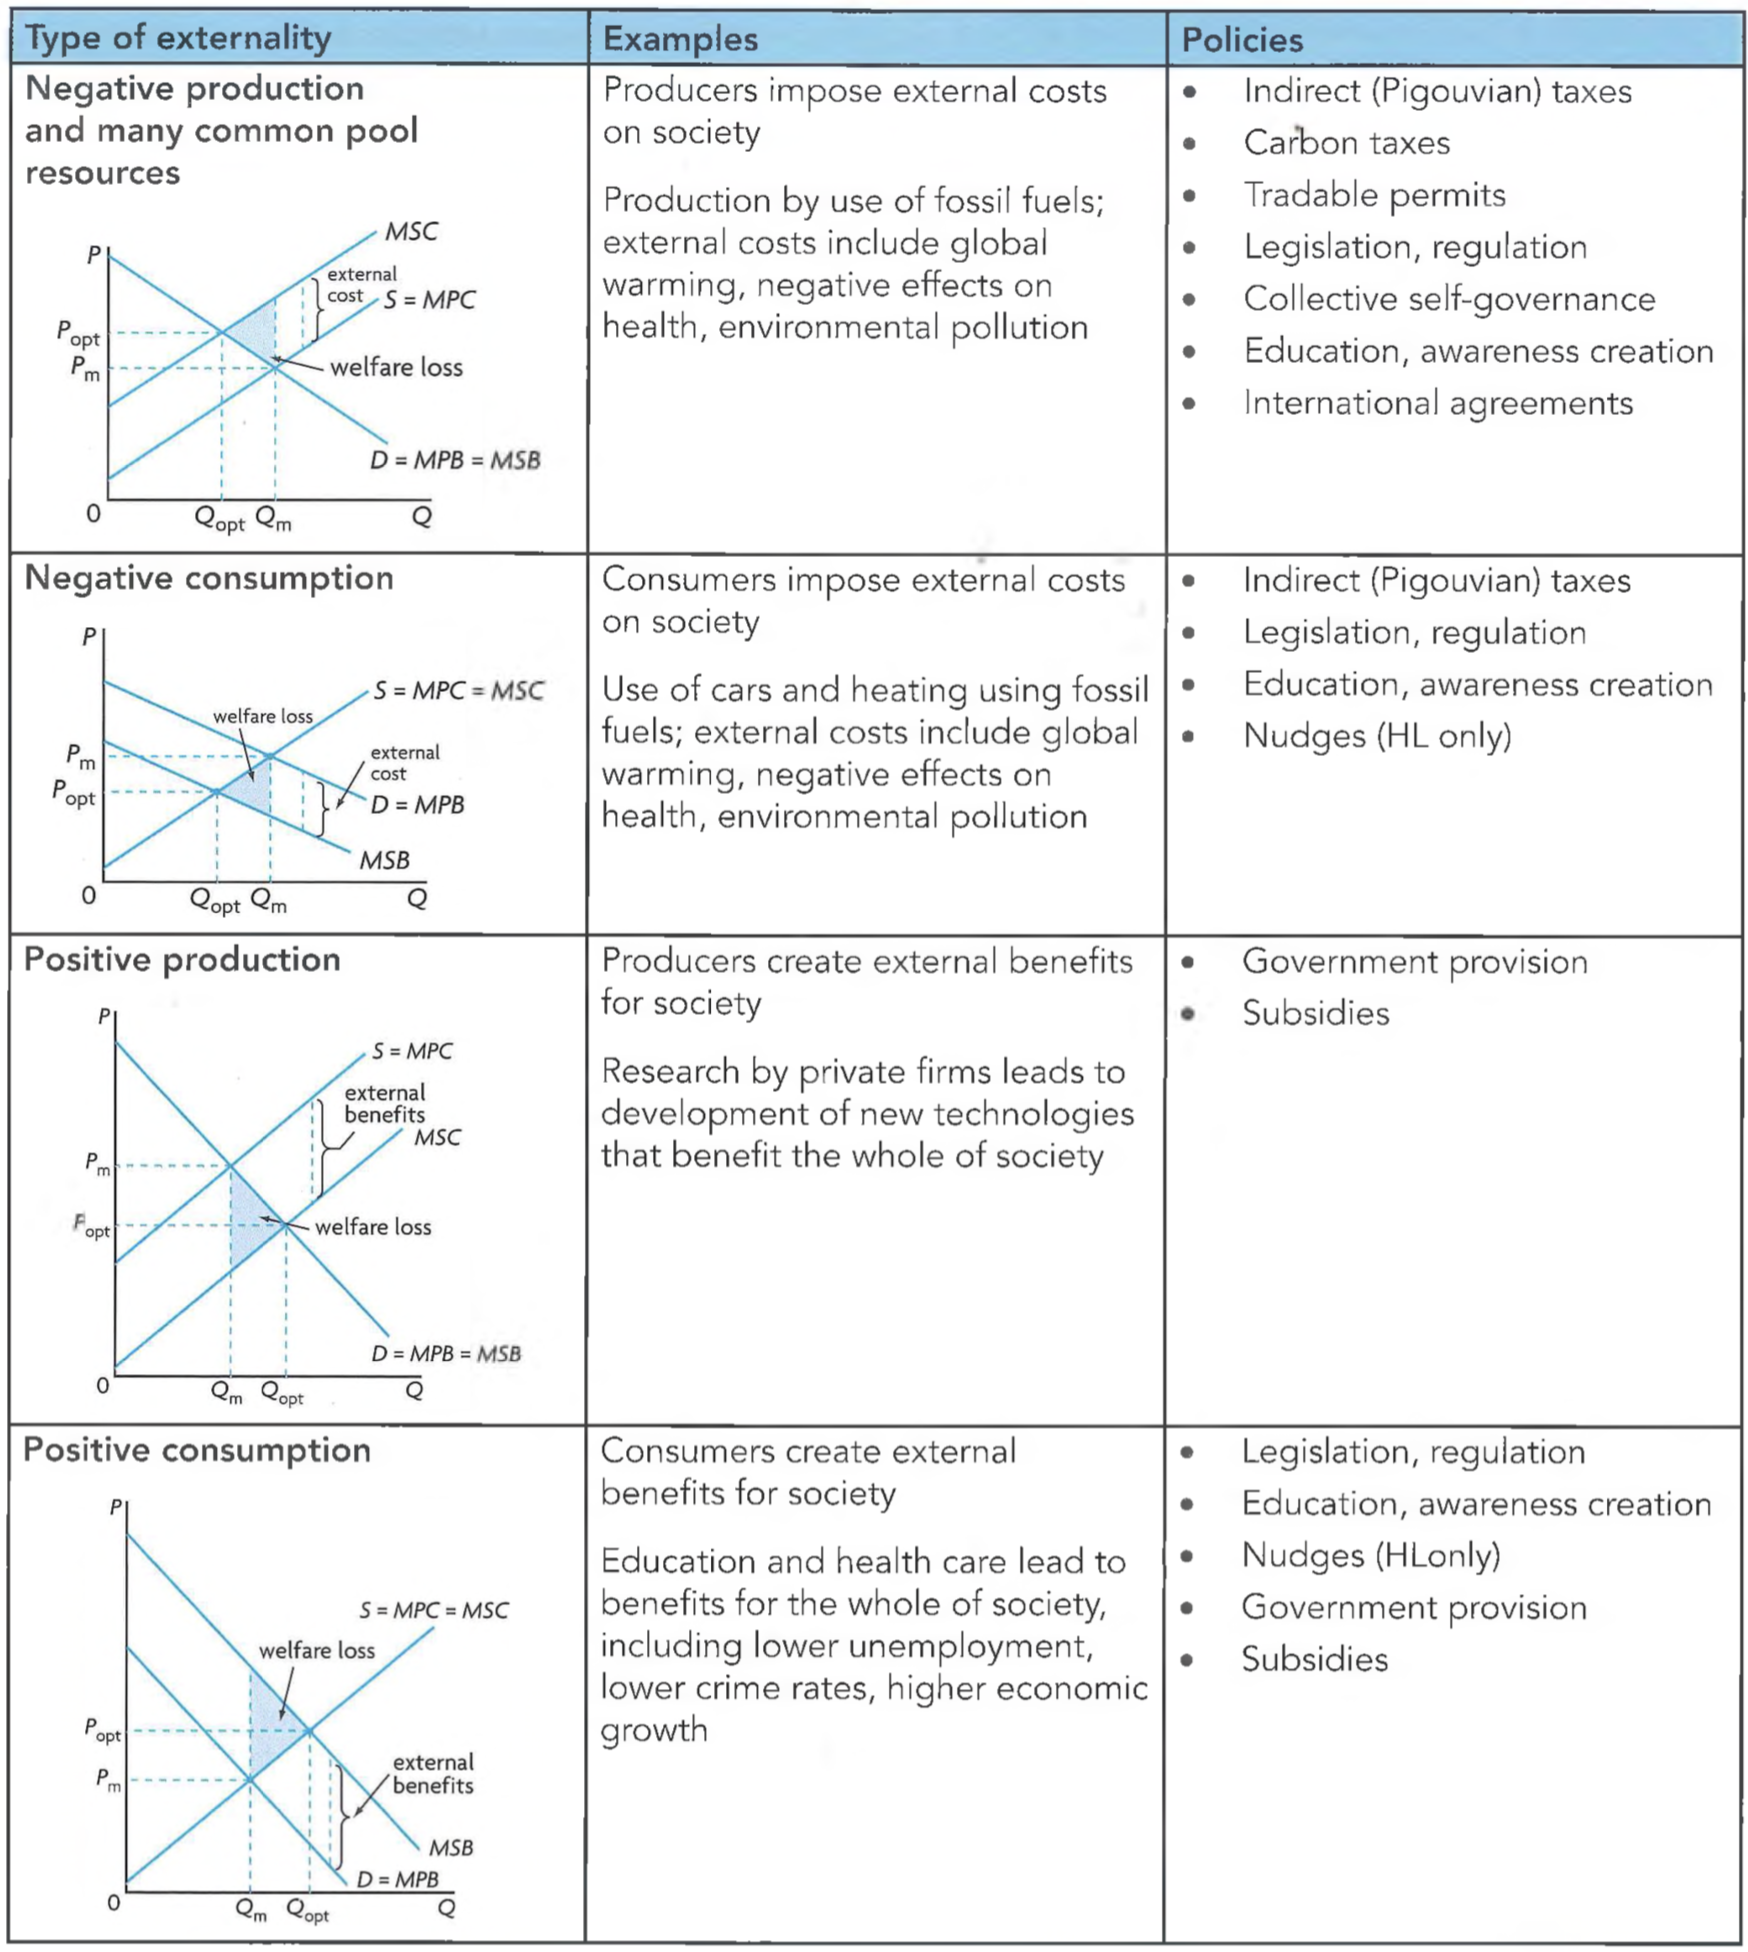
\includegraphics[width=0.99\linewidth]{Screenshot 2026-07-23 at 15.27.46.png}
\end{center}
\begin{itemize}
  \item When there are external costs, MSC > MSB at the point of production by the market.
  \item When there are external benefits MSB > MSC at the point of production by the market.
  \item All production externalities (positive and negative) create a divergence between private and social costs (MPC and MSC).
  \item All consumption externalities (positive and negative) create a divergence between private and social benefits (MPB and MSB).
\end{itemize}
\subsubsection*{Supplementary: The Coase theorem and transaction costs}
\needbold{Coase theorem}: if \textbf{property rights are well defined} and \textbf{transaction costs are low}, private parties can bargain to an efficient (socially optimal) outcome on their own --- even when externalities exist --- because the party that values the right most will buy it. Policy implication: assigning/enforcing property rights (e.g.\ pollution permits) can internalise externalities without direct government regulation. Fails when transaction costs are high, property rights are unclear, or many parties are involved.
\subsubsection*{Supplementary: Transaction costs (AP Ch 11 + Edexcel Book 2 Ch 26)}
\needbold{Transaction costs} are the extra costs involved in making an exchange of goods and services, over and above the price paid. They include:
\begin{itemize}
  \item \textbf{search and information costs} (finding buyers/sellers and learning about quality and prices);
  \item \textbf{bargaining and negotiation costs} (reaching an agreement);
  \item \textbf{monitoring and enforcement costs} (checking performance and enforcing contracts);
  \item in international trade: \textbf{currency conversion fees} and \textbf{exchange-rate risk} --- when countries use different currencies, exporters and importers do not know what the exchange rate will be in the future (under floating rates), and banks charge commissions for conversions.
\end{itemize}
Why transaction costs matter:
\begin{itemize}
  \item \textbf{Market failure / inefficiency}: high transaction costs prevent mutually beneficial exchanges from taking place. In externality problems, when transaction costs are low and property rights are clear, private bargaining can reach the efficient outcome (Coase theorem); when they are high (many affected parties, unclear rights, costly monitoring), the market fails and government intervention may be needed.
  \item \textbf{Trading blocs and monetary union}: a \textbf{monetary union} (single currency) \textbf{eliminates transaction costs} of currency conversion and exchange-rate risk --- a French firm buying from a German firm faces no currency costs, while buying from an American firm still involves currency conversion and exchange-rate risk. This encourages trade, investment and international financial flows. (Tragakes Ch 17.3 estimates euro-zone savings from eliminating these costs at about 1\% of combined GDP.)
\end{itemize}
\subsection{Market failure and public goods}
A \needbold{public good} has the two characteristics:
\begin{itemize}
  \item \needbold{Non-rivalry}: its consumption by one person does not reduce consumption by someone else.
  \item \needbold{Non-excludable}: it is not possible to exclude someone from using the good.
\end{itemize}
Public goods illustrate the \needbold{free rider problem}, occurring when people can enjoy the use of a good without paying for it. The free rider problem arises from non-excludability: people cannot be excluded from using the good. Public goods are a type of market failure because, due to the free rider problem, private firms do not produce these goods: the market fails to allocate resources to their production.
\begin{center}
\begin{tabular}{|p{0.22\linewidth}|p{0.35\linewidth}|p{0.35\linewidth}|}
\hline
 & \textbf{Rivalrous} & \textbf{Non-rivalrous} \\
\hline
\textbf{Excludable} & \textbf{Private goods} & \textbf{Quasi-public goods} \\
 & Goods sold for a price; may have positive or negative externalities (both production and consumption). Includes merit goods (if market-produced) and demerit goods. & Goods that do not fit neatly into the other categories; often have large positive externalities so may be provided by government. \\
\hline
\textbf{Non-excludable} & \textbf{Common pool resources} & \textbf{Public goods} \\
 & Natural resources not owned by anyone, not sold in markets, having no price; lack of price $\to$ overuse, depletion, degradation. & Socially desirable goods not produced by private firms because a price cannot be charged; subject to the \textit{free rider problem}; produced by government and provided free. \\
\hline
\end{tabular}
\end{center}
\subsubsection*{Government intervention to correct the market failure}
\begin{itemize}
  \item \textbf{Direct government provision}: Public goods are \textbf{directly provided}, financed by \textbf{tax revenue}, and made available \textbf{free of charge} (or nearly free).
  \begin{itemize}
    \item Government faces \textbf{choices} on which public goods to provide and in what quantities. Each choice has an OPC.
    \item Unlike private goods, public goods have \textbf{no market price}, so the government cannot easily estimate expected benefits.
    \item \textbf{Cost-benefit analysis}: compares estimated total benefits with total costs. If benefits $>$ costs $\to$ provide; if benefits $<$ costs $\to$ do not provide. The optimal quantity is where $MB = MC$.
    \item \textbf{Difficulties}: costs are relatively easy to estimate, but \textbf{benefits are hard to measure} --- surveys/votes may lead to \textbf{exaggeration} by people who want the good. Cost-benefit analysis is therefore a \textbf{rough and approximate} method.
    \item Provision is also \textbf{political} in nature --- groups compete for benefits, and governments may be swayed by political pressure.
  \end{itemize}
  \item \textbf{Contracting out to the private sector}: the government makes a contract with a private firm to carry out an activity the government would otherwise do itself. Financed by tax revenue.
  \begin{itemize}
    \item \textbf{Pros}:
    \begin{itemize}
      \item \textbf{Competitive tendering} $\to$ lowest-cost provider selected.
      \item Detailed specifications and performance criteria $\to$ potentially \textbf{better quality control}.
      \item Access to \textbf{broader skills and technology} of private firms.
      \item Private firms may be more \textbf{flexible and innovative}.
    \end{itemize}
    \item \textbf{Cons}:
    \begin{itemize}
      \item Government becomes \textbf{less accountable}; \textbf{loses control} over the service.
      \item Private firms may \textbf{charge high prices} $\to$ costs may exceed direct provision.
      \item Competition on cost may \textbf{reduce quality}.
      \item Risk of \textbf{poor contracts} $\to$ higher costs, lower quality, reduced accountability.
      \item \textbf{Monitoring costs} add to government expenditure.
    \end{itemize}
    \item Contracting out only addresses quality/cost/skills issues; it doesn't solve the difficulty of deciding \textit{what} public goods to produce and \textit{how much} (cost-benefit analysis is still needed).
  \end{itemize}
\end{itemize}
\subsection{Asymmetric information}
\needbold{Asymmetric information} refers to something more than just missing information; it refers to situations where buyers and sellers do not have equal access to information.
This usually results in an underallocation of resources to the production of goods or services, and therefore to allocative inefficiency.
\subsubsection*{Adverse selection}
\needbold{Adverse selection} refers to situations where one party in a transaction has more information about the quality of the product being sold than the other party.
\begin{itemize}
  \item Info is ONLY open to sellers:
  \begin{itemize}
    \item In a free unregulated market, the result is usually to underallocate resources to the production of the good or service. Consumers are likely to be aware of possible dangers to themselves, and will be cautious about buying the good or service, resulting in lower demand, less production and lower sales.
    \item However, if consumers are unaware of possible hidden dangers, such as with unsafe food or toys, there could result an overallocation of resources to the production of these goods and services.
  \end{itemize}
  \item According solution:
  \begin{itemize}
      \item \textbf{Government responses:}
      \begin{itemize}
        \item \textbf{Regulation}: laws ensuring quality/safety standards (food, medications, toys, construction). \textit{Difficulties}: time-consuming, bureaucratic, slows economic activity; huge OPC of monitoring across entire supply chains.
        \item \textbf{Provision of information}: government directly supplies information, or forces producers to provide it. \textit{Difficulties}: collecting accurate information has OPC; when private sellers provide information, accuracy is questionable. Some asymmetries cannot be fully eliminated $\to$ \textbf{supplier-induced demand}, where the supplier selectively reveals information to create unnecessary demand.
        \item \textbf{Licensure}: laws requiring proof of competence. \textit{Criticised} for potentially \textbf{limiting supply} in a profession, raising prices and incomes at consumers' expense.
      \end{itemize}
      \item \textbf{Private responses:}
      \begin{itemize}
        \item \textbf{Screening} (by the buyer): the party with limited information tries to learn more about the product/seller (e.g.\ online reviews, asking friends). \textit{Limitation}: cannot provide systematic, complete information to match the seller's knowledge.
        \item \textbf{Signalling} (by the seller): the party with more information tries to convince buyers of good quality (e.g.\ warranties, brand names, service records, fancy showrooms). \textit{Limitation}: unlikely to provide full information; may be inaccurate or misleading if sellers are eager to promote products.
      \end{itemize}
  \end{itemize}
  \item Info is ONLY open to buyers: this situation arises most often in the area of (health) insurance.
  \begin{itemize}
    \item Buyers of health insurance know more about the state of their health than sellers of insurance, and those with health problems are unlikely to tell the full truth to the insurance company.
    \item In a free unregulated market, adverse selection results in an underallocation of resources to health insurance services, as the insurance company reduces the supply of insurance to protect itself.
  \end{itemize}
  \item According solution:
  \begin{itemize}
    \item \textbf{Government responses:}
    \begin{itemize}
      \item \textbf{Direct provision of health care} at low or zero price to the entire population, financed by tax revenue.
      \item \textbf{Social health insurance}: may cover the entire population / selectively cover only vulnerable groups. Ensures no one in need goes without health care.
      \item \textit{Problem}: difficulties in \textbf{controlling costs} and growing burdens on the government/social insurance budget.
    \end{itemize}
    \item \textbf{Private responses:}
    \begin{itemize}
      \item Insurance companies offer a \textbf{range of policies with varying deductibles}: lower-cost policies have \textit{higher} deductibles, higher-cost policies have \textit{lower} deductibles. This is a form of \textbf{screening by the seller}, intended to separate low-risk from high-risk buyers.
      \item \textit{Limitations}: in practice, lower-income earners choose low-cost policies \textit{regardless of health}, creating \textbf{inequity}. Insurance companies also often \textbf{refuse to insure elderly people} (higher risk). The result: those who most need coverage (the poor and elderly) are left with little or no insurance.
    \end{itemize}
  \end{itemize}
\end{itemize}
\subsubsection*{Moral hazard}
\needbold{Moral hazard} refers to situations where one party takes risks, but does not face the full costs of these risks because the full costs of the risks are borne by the other party. In a free, unregulated market, the result of moral hazard is to underallocate resources to the production of (insurance) services.
\subsubsection*{Supplementary: Moral hazard, speculation and market bubbles (Edexcel Book 1 Ch 18)}
Beyond insurance, moral hazard applies to \textbf{speculation and bubbles}: if agents expect prices to keep rising and believe they are protected from losses (e.g.\ bailouts), they take excessive risks $\to$ asset price bubbles (prices far above fundamental values), which burst and cause financial/economic instability. Governments respond with regulation, disclosure requirements and macroprudential policy.
\subsection{Equity in the distribution of income and wealth}
\textbf{Equity} = fairness; \textbf{equality} = sameness. In most countries, the pursuit of equity is understood as reducing significant \textbf{inequalities} in income and wealth, based on the widely shared value judgement that the free market produces unfair inequalities.\\\\
\textbf{Why the market produces unequal incomes}: in a market economy, households' income depends on the \textbf{factors of production they own and sell}, and the \textbf{prices} of those factors. Since ownership of FoPs is \textbf{highly unequal} and factor prices vary enormously:
\begin{itemize}
  \item \textbf{Labour}: most people sell labour for wages, but special skills/education/talents earn very high wages, while the less skilled/educated may earn too little to meet basic needs.
  \item \textbf{Unemployment}: some cannot work (lack of skills, illness, age, disability) or there are not enough jobs.
  \item \textbf{Land, capital, entrepreneurship}: these additional FoPs are \textbf{very unequally distributed}; owners receive rent, interest and profit income.
\end{itemize}
The market \textbf{cannot ensure} everyone receives enough income to satisfy basic needs $\to$ governments intervene to \textbf{redistribute} income and output toward a more socially desirable outcome.\\\\
\textbf{Income vs wealth:}
\begin{itemize}
  \item \textbf{Income}: a \textit{flow} of money received by owners of FoPs (wages, rent, interest, profit).
  \item \textbf{Wealth}: a \textit{stock} of money/assets people \textit{own} (savings, stocks, bonds, land, property, valuables) \textit{minus} debts.
  \item Income and wealth are related (higher income $\to$ more saving $\to$ more wealth), but \textbf{not always closely linked}: high earners may have low wealth (high spenders); pensioners or inheritors may have high wealth but low income.
\end{itemize}
\textbf{Inequality and market failure}: the inability of the market to ensure everyone meets basic needs is \textbf{not strictly market failure}. Market failure is defined as the failure to achieve \textbf{allocative efficiency} ($MSB = MSC$, maximum social surplus). It is possible to have allocative efficiency \textit{and} maximum social surplus even while a large portion of the population is starving; allocative efficiency says nothing about \textbf{for whom} output is distributed.
\begin{center}
  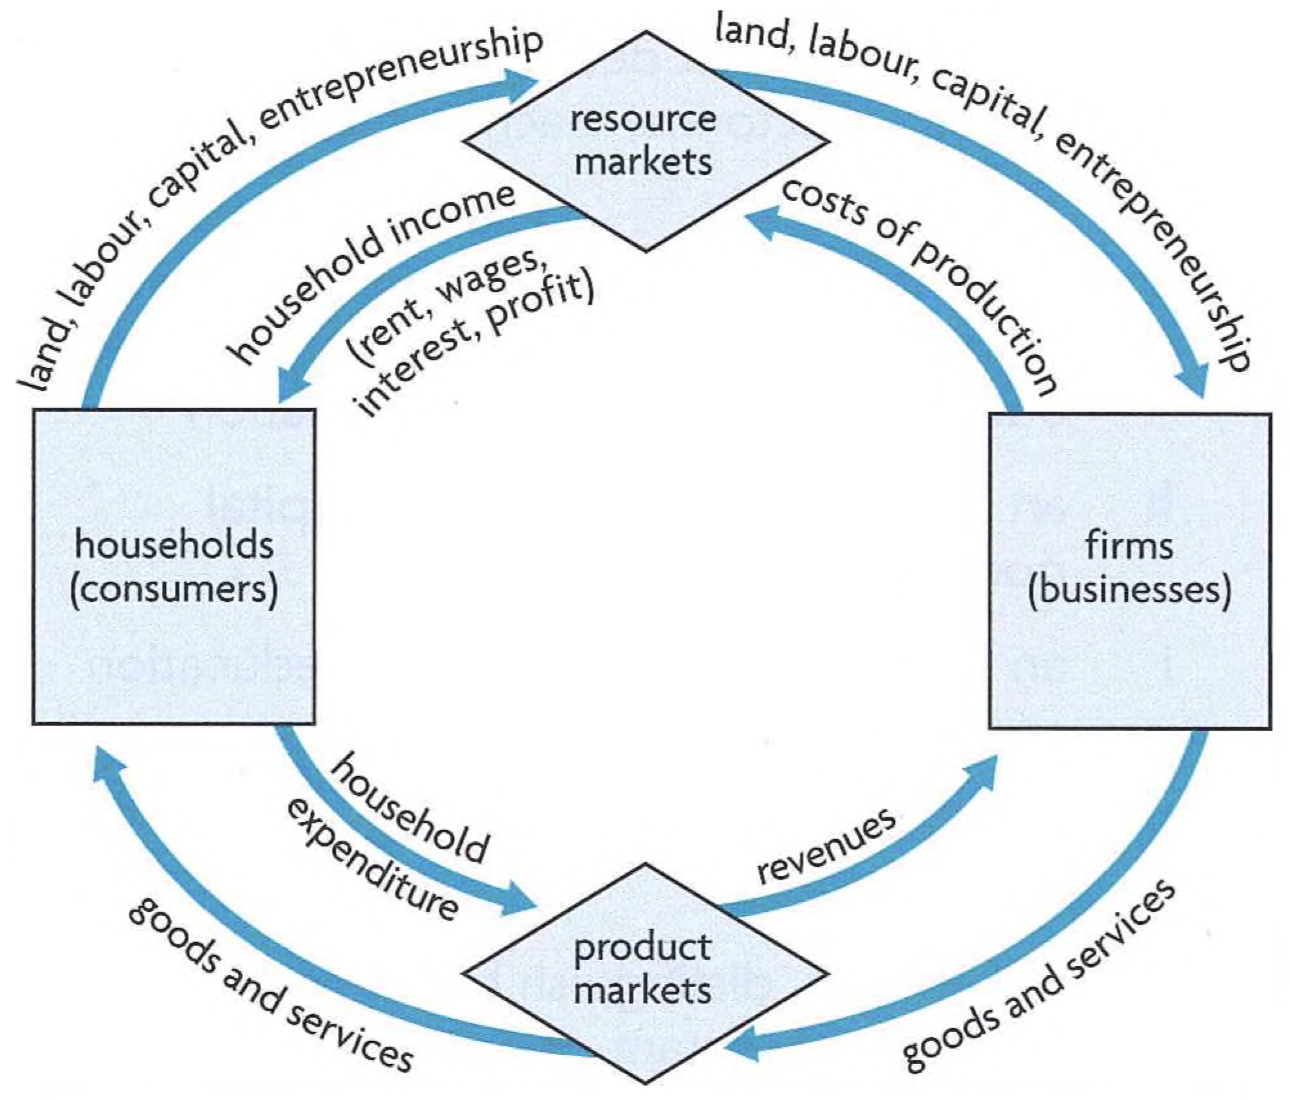
\includegraphics[width=0.55\linewidth]{Screenshot 2026-07-14 at 10.28.33.png}
\end{center}
\section{Market failure and socially undesirable outcomes III}
\subsection{Introduction to firms, industries and market structures}
Industries are analysed by use of models called \needbold{market structures}, which describe characteristics of a market organisation that determine the behaviour of firms.
\\\needbold{Market power}: the extent to which each individual firm in the industry is able to control the price at which it sells its product.\\
Market structure is defined based on these indicators:
\begin{itemize}
  \item the number of firms in the industry
  \item product differentiation: how similar or different are the goods or services produced
  \item barriers to entry: how easy or difficult it is for new firms to enter the industry and begin producing
\end{itemize}
Types of market structures to be studied:
\begin{itemize}
  \item Perfect competition: firms have no ability to control the price of their products; (price takers) such firms have zero market power.
  \begin{itemize}
    \item There is a very large number of firms in the industry.
    \item All the firms in the industry sell homogenous products.
    \item There are no barriers to entry.
\item Buyers and sellers know every price and every product.
  \end{itemize}
  \item Monopolistic competition
  \begin{itemize}
    \item There is a fairly large number of small (or medium-­sized) firms in the industry.
    \item There are no barriers to entry.
    \item There is product differentiation.
  \end{itemize}
  \item Oligopoly
  \begin{itemize}
    \item There is a small number of large firms in the industry, the firms are interdependent (form cartels).
    \item Products may be either differentiated (cars) or undifferentiated (oil).
    \item There are high barriers to entry.
  \end{itemize}
  \item Monopoly: there is single firm in the market; this firm has the greatest ability to control the price of its product, and therefore the greatest amount of market power.
  \begin{itemize}
    \item There is a single seller or dominant firm in the industry, so the single firm is the entire industry.
    \item The firm produces and sells a unique good or service, with no close substitutes.
    \item There are high barriers to entry in the industry.
  \end{itemize}
\end{itemize}
Firms in the other three market structures (other than perfect competition) result in market failure to varying degrees, with monopoly resulting in the greatest degree of allocative inefficiency.\\
\begin{center}
\renewcommand{\arraystretch}{1.6}
\begin{tabular}{|p{0.14\linewidth}|p{0.13\linewidth}|p{0.15\linewidth}|p{0.12\linewidth}|p{0.13\linewidth}|p{0.13\linewidth}|}
\hline
 & \textbf{Number of firms} & \textbf{Type of product} & \textbf{Ease of entry} & \textbf{Market power / control over price} & \textbf{Degree of competition} \\
\hline
\textbf{Perfect competition} & very many, very small & homogeneous / undifferentiated & very easy & none & perfect \\
\hline
\textbf{Monopolistic competition} & relatively many, relatively small & differentiated & very easy & some & a good amount \\
\hline
\textbf{Oligopoly} & few large & differentiated or undifferentiated & very difficult & significant & some (but far less than monopolistic competition) \\
\hline
\textbf{Monopoly} & one, large & one product with no close substitutes & difficult to impossible & very significant & none \\
\hline
\end{tabular}
\end{center}
\subsection{Profit maximisation by the rational producer}
\subsubsection*{Revenue}
\needbold{Revenues} are the payments firms receive when they sell the goods and services they produce. 
\begin{itemize}
  \item Total revenue, $TR=Q\times P$ maximized where $PED = 1$ and $MR = 0$.
  \item Average revenue, $AR=\dfrac{TR}{Q}=P$ 
  \item Marginal revenue, $MR=\dfrac{\Delta TR}{\Delta Q}$
\end{itemize}
Revenues in two different types of markets:
\begin{itemize}
  \item Perfect competition: the firm is unable to control price; price is constant as output varies
  \item Monopolistic competition, Oligopoly, Monopoly: the firm has control over price; price varies with output
\end{itemize}
\textbf{Perfect competition: revenue data} (price is constant; $P = AR = MR$):
\begin{center}
\begin{tabular}{ccccc}
\toprule
$Q$ & $P$ & $TR$ & $AR$ & $MR$ \\
\midrule
0 & 10 & 0  & 10 & 10 \\
1 & 10 & 10 & 10 & 10 \\
2 & 10 & 20 & 10 & 10 \\
3 & 10 & 30 & 10 & 10 \\
4 & 10 & 40 & 10 & 10 \\
5 & 10 & 50 & 10 & 10 \\
6 & 10 & 60 & 10 & 10 \\
\bottomrule
\end{tabular}
\end{center}
\begin{center}
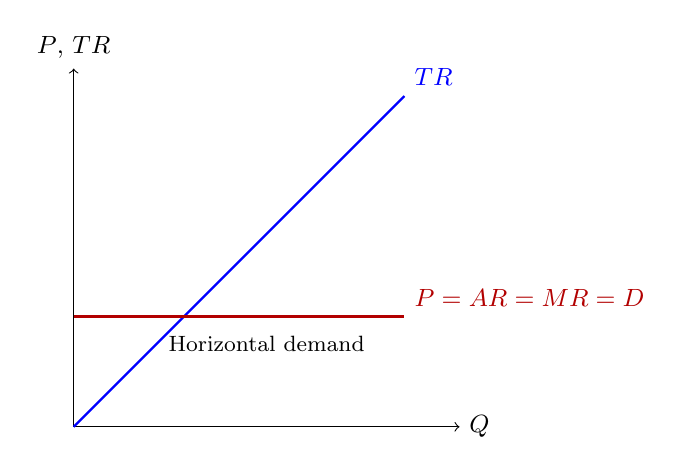
\begin{tikzpicture}[scale=0.7]
\draw[->] (0,0) -- (7,0) node[right, font=\small] {$Q$};
\draw[->] (0,0) -- (0,6.5) node[above, font=\small] {$P$, $TR$};
% TR line: TR = 10Q
\draw[thick, blue] (0,0) -- (6,6) node[above right, blue, font=\small] {$TR$};
% P = AR = MR horizontal line at P=10
\draw[thick, red!70!black] (0,2) -- (6,2) node[above right, red!70!black, font=\small] {$P = AR = MR = D$};
\node[font=\footnotesize] at (3.5,1.5) {Horizontal demand};
\end{tikzpicture}
\end{center}
In perfect competition, $P = AR = MR$ is a \textbf{horizontal line} (the firm is a price taker), and $TR$ is an \textbf{upward-sloping straight line} through the origin ($TR = P \times Q$).\\
\textbf{Imperfect competition (monopoly, monopolistic competition, oligopoly): revenue data} (firm faces downward-sloping demand; $P = AR > MR$):
\begin{center}
\begin{tabular}{ccccc}
\toprule
$Q$ & $P = AR$ & $TR$ & $AR$ & $MR$ \\
\midrule
0 & 11 & 0  & --- & --- \\
1 & 10 & 10 & 10 & 10 \\
2 & 9  & 18 & 9  & 8 \\
3 & 8  & 24 & 8  & 6 \\
4 & 7  & 28 & 7  & 4 \\
5 & 6  & 30 & 6  & 2 \\
6 & 5  & 30 & 5  & 0 \\
7 & 4  & 28 & 4  & $-2$ \\
\bottomrule
\end{tabular}
\end{center}
\begin{center}
\begin{tikzpicture}[scale=1.1]
\draw[->] (0,0) -- (7,0) node[right, font=\small] {$Q$};
\draw[->] (0,0) -- (0,6.5) node[above, font=\small] {$P$, $TR$};
% TR curve: inverted parabola
\draw[thick, blue, domain=0:7, samples=50] plot (\x, {0.65*\x*(7-\x)/7*2});
\node[blue, font=\small] at (5.2,2.6) {$TR$};
% AR = P = D line (downward sloping)
\draw[thick, red!70!black] (0,5.5) -- (6,0.5) node[below right, red!70!black, font=\small] {$P = AR = D$};
% MR line (steeper downward)
\draw[thick, green!50!black, dashed] (0,5.5) -- (3.5,0.5) -- (4.8,-1.1);
\node[green!50!black, font=\small] at (3.8,1.3) {$MR$};
\end{tikzpicture}
\end{center}
\subsubsection*{Costs of production}
When firms use inputs or resources to produce, they incur CoP which include money payments
to buy resources plus anything else given up by a firm for the use of resources.
\begin{itemize}
  \item Such payments made by a firm to outsiders to acquire resources for use in production are known as \needbold{explicit costs}.
  \item The sacrificed income arising from the use of self-owned resources by a firm is an \needbold{implicit cost}. (Considered as OPC?)
\end{itemize}
The sum of explicit and implicit costs incurred by a firm for its use of resources, whether purchased or self-owned, are known as \needbold{economic costs}.\\
Different types of cost: 
\begin{itemize}
  \item Total cost, $TC$, all the CoP incurred by a firm
  \item Marginal cost, $MC=\dfrac{\Delta TC}{\Delta Q}$
  \item Average cost, $AC=\dfrac{TC}{Q}$
\end{itemize}
Cost of production under short run and long run:
\begin{itemize}
  \item In the short run: the period of time when at least one factor of production is fixed\\
  \textbf{Key relationship between $MC$ and $AC$}:
\begin{itemize}
  \item When $MC < AC$, $AC$ is \textbf{falling} (the extra unit costs less than the average, pulling the average down).
  \item When $MC > AC$, $AC$ is \textbf{rising} (the extra unit costs more than the average, pulling the average up).
  \item When $MC = AC$, $AC$ is at its \textbf{minimum} ($MC$ cuts $AC$ at its lowest point).
  \item The same relationship holds between $MC$ and $AVC$ (average variable cost).
\end{itemize}
 
\begin{center}
\begin{tikzpicture}[scale=1]
\draw[->] (0,0) -- (7,0) node[right, font=\small] {Output ($Q$)};
\draw[->] (0,0) -- (0,5.5) node[above, font=\small] {Cost};
% MC curve: U-shaped, steep at first, falling then rising sharply
\draw[thick, red!70!black] plot[domain=0.6:6, samples=50] (\x, {0.4*(\x-2.2)^2 + 0.8});
\node[red!70!black, font=\small] at (5.5,3.5) {$MC$};
% AC curve: U-shaped, higher and flatter than MC
\draw[thick, blue] plot[domain=0.6:6.2, samples=50] (\x, {0.3*(\x-3)^2 + 1.5});
\node[blue, font=\small] at (5.6,2.8) {$AC$};
\end{tikzpicture}
\end{center}
 \item In the long run: the period of time when all factors of production are variable (increases all FoPs)
\end{itemize}

\begin{center}
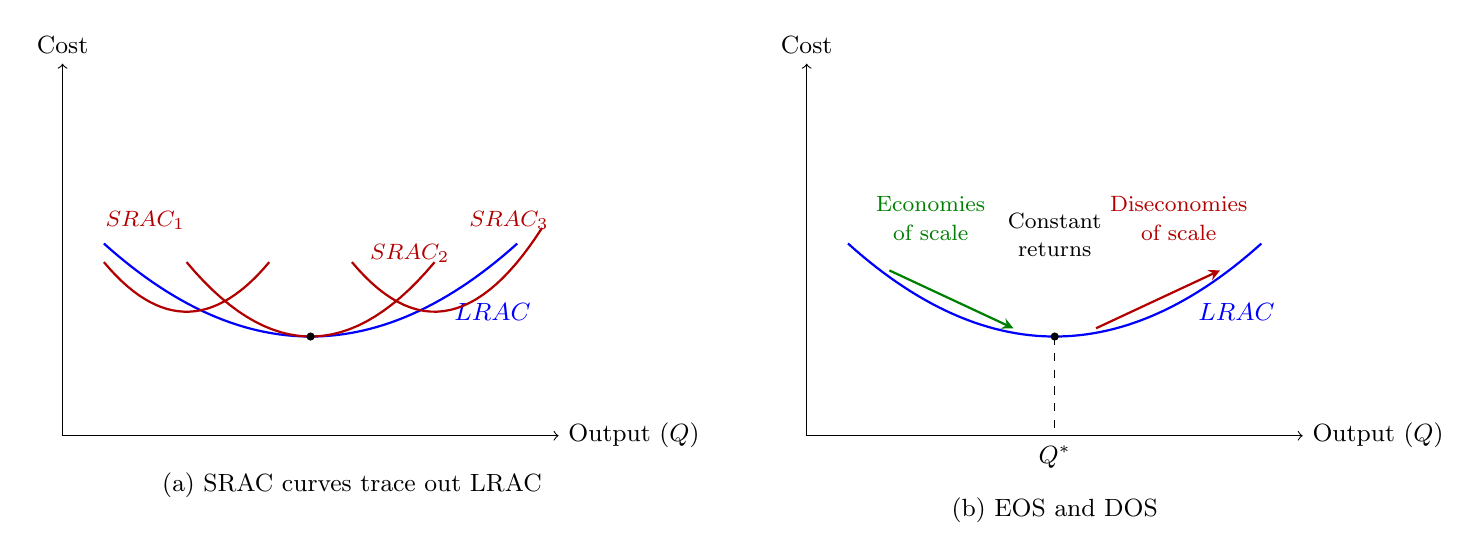
\begin{tikzpicture}[scale=1.05]
% --- (a) LRAC with SRAC curves ---
\begin{scope}
\draw[->] (0,0) -- (6,0) node[right, font=\small] {Output ($Q$)};
\draw[->] (0,0) -- (0,4.5) node[above, font=\small] {Cost};
% LRAC curve (U-shaped, broad)
\draw[thick, blue, domain=0.5:5.5, samples=60] plot (\x, {0.18*(\x-3)^2 + 1.2});
\node[blue, font=\small] at (5.2,1.5) {$LRAC$};
% SRAC1 (left, higher min)
\draw[thick, red!70!black, domain=0.5:2.5, samples=30] plot (\x, {0.6*(\x-1.5)^2 + 1.5});
\node[red!70!black, font=\footnotesize] at (1.0,2.6) {$SRAC_1$};
% SRAC2 (middle, lowest, tangent at LRAC minimum)
\draw[thick, red!70!black, domain=1.5:4.5, samples=30] plot (\x, {0.4*(\x-3)^2 + 1.2});
\node[red!70!black, font=\footnotesize] at (4.2,2.2) {$SRAC_2$};
% SRAC3 (right, higher min)
\draw[thick, red!70!black, domain=3.5:5.8, samples=30] plot (\x, {0.6*(\x-4.5)^2 + 1.5});
\node[red!70!black, font=\footnotesize] at (5.4,2.6) {$SRAC_3$};
% Minimum LRAC point
\filldraw (3.0,1.2) circle (1.2pt);
\node[font=\small] at (3.5,-0.6) {(a) SRAC curves trace out LRAC};
\end{scope}
% --- (b) Economies and diseconomies of scale ---
\begin{scope}[xshift=9cm]
\draw[->] (0,0) -- (6,0) node[right, font=\small] {Output ($Q$)};
\draw[->] (0,0) -- (0,4.5) node[above, font=\small] {Cost};
% LRAC curve
\draw[thick, blue, domain=0.5:5.5, samples=60] plot (\x, {0.18*(\x-3)^2 + 1.2});
\node[blue, font=\small] at (5.2,1.5) {$LRAC$};
% Minimum point
\filldraw (3.0,1.2) circle (1.2pt);
\draw[dashed] (3.0,1.2) -- (3.0,0) node[below, font=\small] {$Q^*$};
% Regions
\node[green!50!black, font=\footnotesize] at (1.5,2.8) {Economies};
\node[green!50!black, font=\footnotesize] at (1.5,2.45) {of scale};
\node[font=\footnotesize] at (3.0,2.6) {Constant};
\node[font=\footnotesize] at (3.0,2.25) {returns};
\node[red!70!black, font=\footnotesize] at (4.5,2.8) {Diseconomies};
\node[red!70!black, font=\footnotesize] at (4.5,2.45) {of scale};
% Arrow indicating falling then rising
\draw[->, >=stealth, thick, green!50!black] (1.0,2.0) -- (2.5,1.3);
\draw[->, >=stealth, thick, red!70!black] (3.5,1.3) -- (5.0,2.0);
\node[font=\small] at (3.0,-0.9) {(b) EOS and DOS};
\end{scope}
\end{tikzpicture}
\end{center}
\needbold{Economies of scale}: decreases in average costs of production over the long run as a firm increases all its factors of production.\\
Reasons for EoS to occur:
\begin{itemize}
  \item Specialization of labor (labor economies)
  \item Specialization of management (managerial economies)
  \item Bulk buying of inputs / FoPs (buying economies)
  \item Financing economies
  \item Spreading of certain costs, such as marketing, over larger volumes of output. (risk-bearing economies)
\end{itemize}
\needbold{Diseconomies of scale}: increases in the average costs of production in the long run as a firm increases its output by increasing all its inputs.\\
Reasons for DisEoS to occur: 
\begin{itemize}
  \item Co-ordination and monitoring difficulties
  \item Communication difficulties
  \item Poor worker motivation
\end{itemize}
\subsubsection*{Profit}
In general, profit = total revenue - economic cost (explicit costs + implicit costs).\\
\needbold{Profit maximization}: determining the level of output that the firm should produce to make profit as large as possible.\\
Two approaches to analyze profit maximization:
\begin{itemize}
  \item Total revenue - Total cost (economic costs fundamentally), make this value as large as possible
  \begin{itemize}
    \item Positive profit: TR > TC, earns abnormal profit
    \item Zero profit: TR = TC, earns normal profit (the minimum amount of revenue that the firm must receive so that it will keep the business running / the amount of revenue that covers all explicit and implicit costs)
    \item Negative profit: TR < TC, incurs a loss
  \end{itemize}
  \item Marginal revenue = Marginal cost (produces at this level of output to achieve profit maximization)
  \begin{itemize}
    \item MR > MC, underproduced at the moment
    \item MR < MC, overproduced at the moment
    \item MR = MC, profit maximizing level of output
  \end{itemize}
\end{itemize}
\subsubsection*{Supplementary: Costs of production, returns to scale and profit (AP Barron Ch 6)}
\begin{itemize}
  \item \needbold{Accounting profit} $= TR - \text{explicit costs}$; \needbold{economic profit} $= TR - \text{(explicit + implicit costs)}$. Economic profit is always $\leq$ accounting profit. Zero economic profit (\textbf{normal profit}) still yields positive accounting profit, covering the opportunity costs of self-owned resources.
  \item \needbold{Average product} $AP = TP/L$ (output per unit of labour); \needbold{marginal product} $MP = \Delta TP/\Delta L$. When $MP > AP$, $AP$ rises; when $MP < AP$, $AP$ falls; $MP = AP$ at $AP$'s maximum (the mirror image of the MC and AC relationship).
  \item \needbold{Returns to scale} (long run): increasing returns to scale (output rises proportionally more than all inputs) $\to$ falling LRAC; constant returns to scale $\to$ flat LRAC; decreasing returns to scale $\to$ rising LRAC.
  \item \needbold{Minimum efficient scale (MES)}: the lowest level of output at which long-run average cost ($LRAC$) reaches its minimum. Firms producing below MES suffer from higher average costs (relevant for excess capacity in monopolistic competition).
  \item \needbold{Internal economies of scale} arise from the firm's own growth in size (technical, managerial, financial, bulk-buying, risk-bearing); \needbold{external economies of scale} arise from the expansion of the entire industry (access to specialized suppliers, skilled labour pools, industry-specific infrastructure).
\end{itemize}
\subsection{Perfect competition}
\begin{itemize}
  \item The demand curve for a good facing the perfectly competitive firm is perfectly elastic (horizontal) at the price determined in the market for that good. This means the firm is a price-taker, as it accepts the price determined in the market. The firm has no ability to influence price therefore it has no market power.
  \item No matter how much output the perfectly competitive firm sells, P = MR = AR and these are constant at the level of the horizontal demand curve. This follows from the fact that price is constant regardless of the level of output sold.
  \item When the profit maximizing quantity $Q_{max}$ is determined using MC = MR:
  \begin{itemize}
    \item If AR > AC (or P > AC), the firm makes abnormal profit.
    \item If AR = AC (or P = AC), the firm makes normal profit.
    \item If AR < AC (or P < AC), the firm makes a loss.
  \end{itemize}
\end{itemize}
In the short run:
\begin{center}
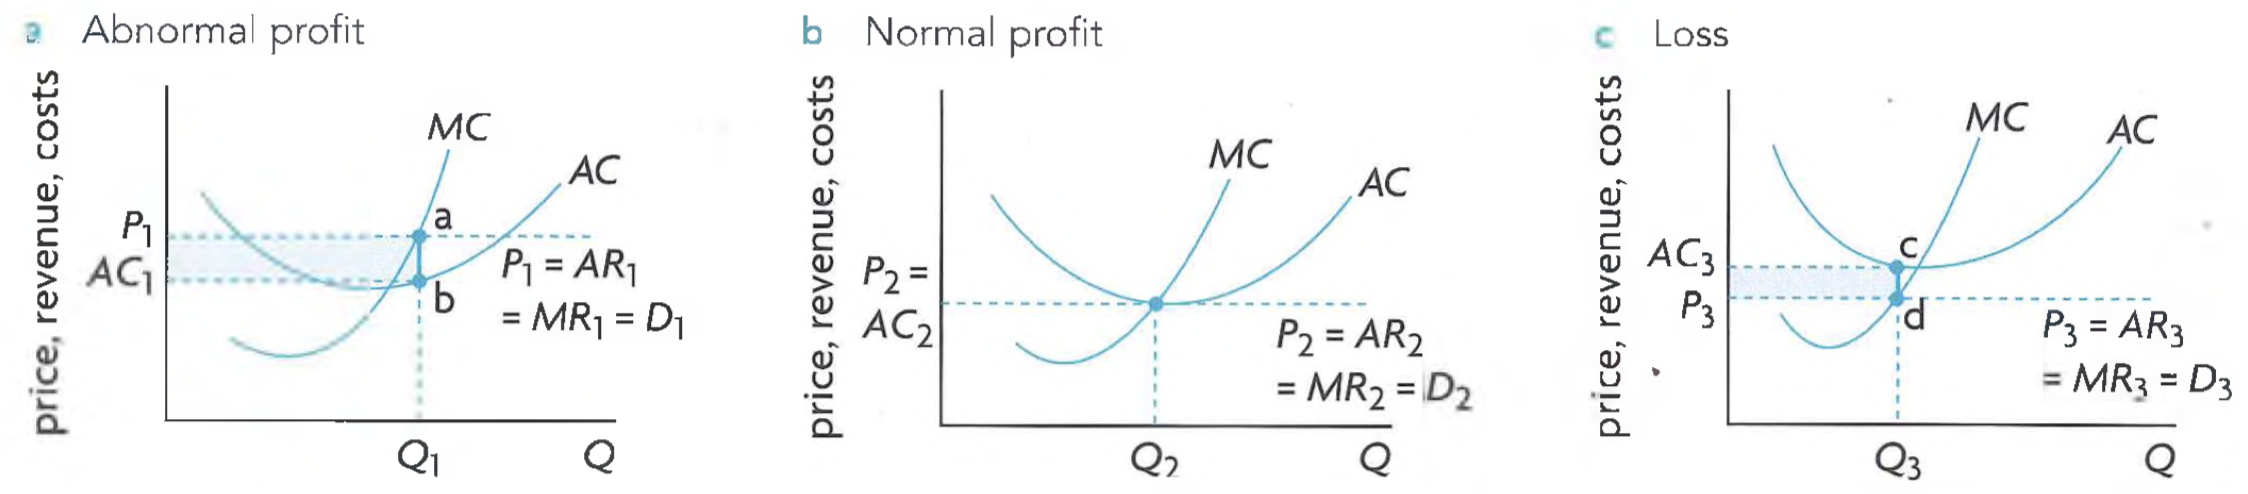
\includegraphics[width=0.95\linewidth]{Screenshot 2026-07-24 at 11.05.22.png}
\end{center}
\subsubsection*{Supplementary: The shut-down rule (AP Barron Ch 7)}
In the short run, a loss-making firm decides whether to continue operating by comparing price ($P$) with \textbf{average variable cost ($AVC$)}, not $ATC$:
\begin{itemize}
  \item $P > ATC$: firm earns abnormal profit.
  \item $AVC < P < ATC$: operate at a \textbf{loss} in the short run (losses are smaller than fixed costs if it continues producing, because revenue covers all variable costs and contributes toward paying fixed costs).
  \item $P < AVC$: \textbf{shut down immediately} (operating losses exceed total fixed costs).
  \item Thus, the perfectly competitive firm's short-run \textbf{supply curve is the marginal cost ($MC$) curve above the minimum point of $AVC$}.
\end{itemize}
In the long-run equilibrium of perfect competition, all firms earn zero profit. Firms' profits and losses are eliminated (due to firms joining and quitting in the industry, causing industry supply curve to change, leading the price to change), and revenues are just enough to cover all costs so that every firm earns normal profit.
\begin{center}
  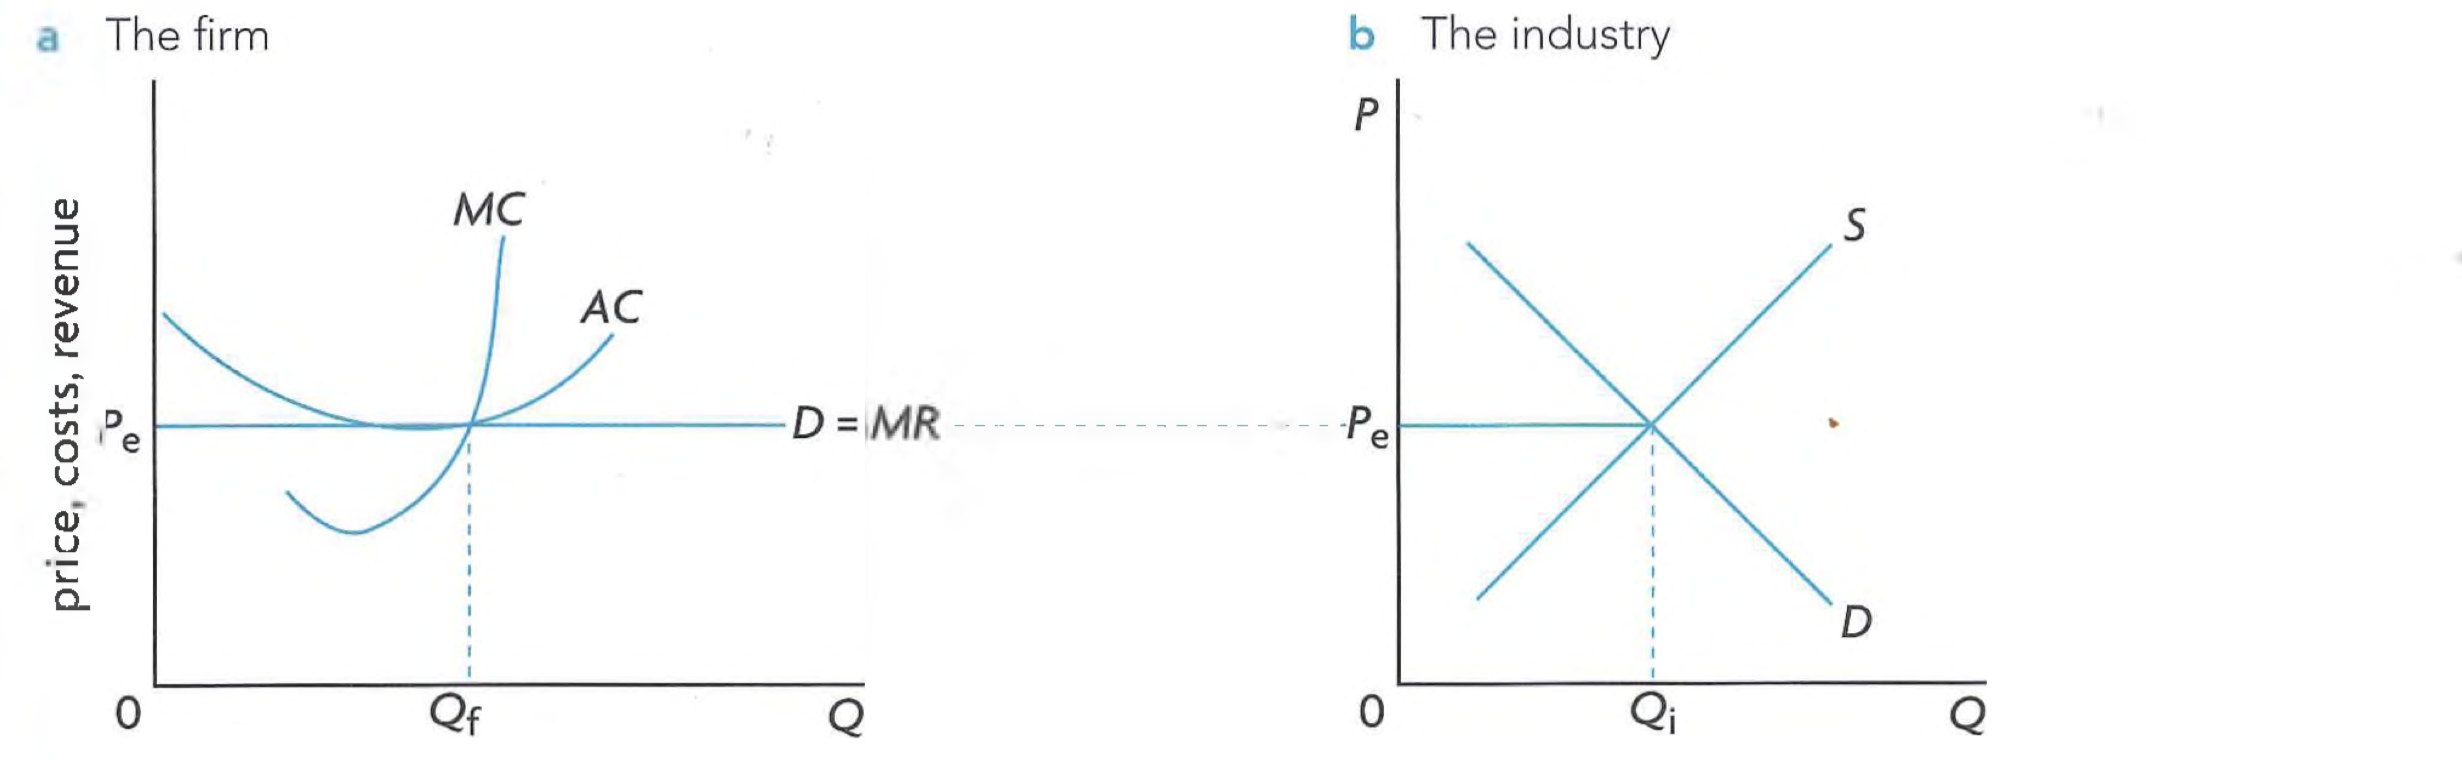
\includegraphics[width=0.8\linewidth]{Screenshot 2026-07-24 at 11.06.42.png}
\end{center}
\subsubsection*{From short-run equilibrium to long-run equilibrium (supplementary)}
\textbf{Abnormal profit in the short run $\to$ normal profit in the long run}:
\begin{enumerate}
  \item In the short run, price $P_1 >$ minimum ATC, so firms earn abnormal profit (per-unit profit $= a - b$ in the textbook figure).
  \item Abnormal profit attracts \textbf{entry of new firms} into the industry.
  \item Industry supply $S_1$ shifts \textbf{right} to $S_2$; industry output rises from $Q_1$ to $Q_2$ and market price falls from $P_1$ to $P_2$.
  \item Entry continues until abnormal profit is competed away: at $P_2$, every firm earns \textbf{normal profit} where $P = $ minimum ATC.
\end{enumerate}
\textbf{Losses in the short run $\to$ normal profit in the long run}:
\begin{enumerate}
  \item In the short run, price $P_1 <$ minimum ATC, so firms make losses (loss per unit $= a - b$ in the textbook figure).
  \item In the long run, firms are free to leave the industry; as some \textbf{exit}, industry supply $S_1$ shifts \textbf{left} to $S_2$.
  \item Price rises from $P_1$ to $P_2$; remaining firms' losses shrink until, at $P_2$, they earn \textbf{normal profit} ($P = $ minimum ATC).
\end{enumerate}
\begin{center}
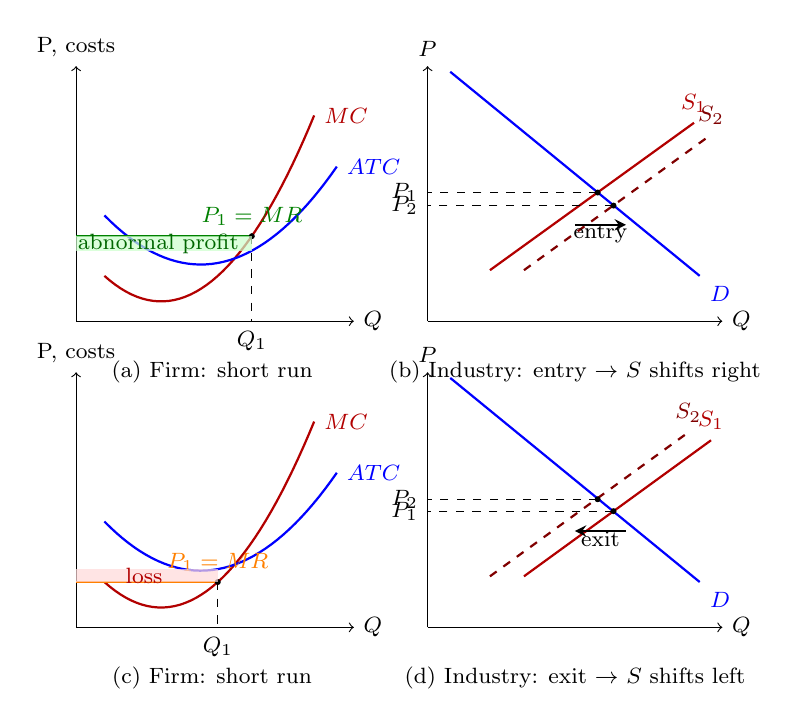
\begin{tikzpicture}[scale=0.72]
% Row 1: abnormal profit in SR -> entry -> normal profit in LR
\begin{scope}
\draw[->] (0,0) -- (4.9,0) node[right, font=\footnotesize] {$Q$};
\draw[->] (0,0) -- (0,4.5) node[above, font=\footnotesize] {P, costs};
\draw[thick, red!70!black] plot[domain=0.5:4.2, samples=40] (\x, {0.45*(\x-1.5)^2+0.35}) node[right, red!70!black, font=\footnotesize] {$MC$};
\draw[thick, blue] plot[domain=0.5:4.6, samples=40] (\x, {0.3*(\x-2.2)^2+1.0}) node[right, blue, font=\footnotesize] {$ATC$};
\draw[thick, green!50!black] (0,1.5) -- (3.1,1.5) node[above, green!50!black, font=\footnotesize] {$P_1 = MR$};
\filldraw (3.1,1.5) circle (1.2pt);
\draw[dashed] (3.1,1.5) -- (3.1,0) node[below, font=\footnotesize] {$Q_1$};
\fill[green!20, opacity=0.7] (0,1.24) rectangle (3.1,1.5);
\node[font=\footnotesize, green!40!black] at (1.45,1.37) {abnormal profit};
\node[font=\footnotesize, align=center] at (2.4,-0.9) {(a) Firm: short run};
\end{scope}
\begin{scope}[xshift=6.2cm]
\draw[->] (0,0) -- (5.2,0) node[right, font=\footnotesize] {$Q$};
\draw[->] (0,0) -- (0,4.5) node[above, font=\footnotesize] {$P$};
\draw[thick, blue] (0.4,4.4) -- (4.8,0.8) node[below right, blue, font=\footnotesize] {$D$};
\draw[thick, red!70!black] (1.1,0.9) -- (4.7,3.5) node[above, red!70!black, font=\footnotesize] {$S_1$};
\draw[thick, red!50!black, dashed] (1.7,0.9) -- (5.0,3.29) node[above, red!50!black, font=\footnotesize] {$S_2$};
\filldraw (3.0,2.27) circle (1.2pt);
\filldraw (3.28,2.04) circle (1.2pt);
\draw[dashed] (3.0,2.27) -- (0,2.27) node[left, font=\footnotesize] {$P_1$};
\draw[dashed] (3.28,2.04) -- (0,2.04) node[left, font=\footnotesize] {$P_2$};
\draw[->, >=stealth, thick] (2.6,1.7) -- (3.5,1.7);
\node[font=\footnotesize] at (3.05,1.55) {entry};
\node[font=\footnotesize, align=center] at (2.6,-0.9) {(b) Industry: entry $\to$ $S$ shifts right};
\end{scope}
% Row 2: losses in SR -> exit -> normal profit in LR
\begin{scope}[yshift=-5.4cm]
\draw[->] (0,0) -- (4.9,0) node[right, font=\footnotesize] {$Q$};
\draw[->] (0,0) -- (0,4.5) node[above, font=\footnotesize] {P, costs};
\draw[thick, red!70!black] plot[domain=0.5:4.2, samples=40] (\x, {0.45*(\x-1.5)^2+0.35}) node[right, red!70!black, font=\footnotesize] {$MC$};
\draw[thick, blue] plot[domain=0.5:4.6, samples=40] (\x, {0.3*(\x-2.2)^2+1.0}) node[right, blue, font=\footnotesize] {$ATC$};
\draw[thick, orange] (0,0.8) -- (2.5,0.8) node[above, orange, font=\footnotesize] {$P_1 = MR$};
\filldraw (2.5,0.8) circle (1.2pt);
\draw[dashed] (2.5,0.8) -- (2.5,0) node[below, font=\footnotesize] {$Q_1$};
\fill[red!15, opacity=0.7] (0,0.8) rectangle (2.5,1.03);
\node[font=\footnotesize, red!70!black] at (1.2,0.91) {loss};
\node[font=\footnotesize, align=center] at (2.4,-0.9) {(c) Firm: short run};
\end{scope}
\begin{scope}[xshift=6.2cm, yshift=-5.4cm]
\draw[->] (0,0) -- (5.2,0) node[right, font=\footnotesize] {$Q$};
\draw[->] (0,0) -- (0,4.5) node[above, font=\footnotesize] {$P$};
\draw[thick, blue] (0.4,4.4) -- (4.8,0.8) node[below right, blue, font=\footnotesize] {$D$};
\draw[thick, red!70!black] (1.7,0.9) -- (5.0,3.3) node[above, red!70!black, font=\footnotesize] {$S_1$};
\draw[thick, red!50!black, dashed] (1.1,0.9) -- (4.6,3.44) node[above, red!50!black, font=\footnotesize] {$S_2$};
\filldraw (3.28,2.05) circle (1.2pt);
\filldraw (3.0,2.26) circle (1.2pt);
\draw[dashed] (3.28,2.05) -- (0,2.05) node[left, font=\footnotesize] {$P_1$};
\draw[dashed] (3.0,2.26) -- (0,2.26) node[left, font=\footnotesize] {$P_2$};
\draw[->, >=stealth, thick] (3.5,1.7) -- (2.6,1.7);
\node[font=\footnotesize] at (3.05,1.55) {exit};
\node[font=\footnotesize, align=center] at (2.6,-0.9) {(d) Industry: exit $\to$ $S$ shifts left};
\end{scope}
\end{tikzpicture}
\end{center}
Both adjustment processes are driven by the \textbf{MC = MR} rule at every stage.
\subsubsection*{Allocative efficiency}
\needbold{Allocative efficiency} occurs when firms produce the particular combination of goods and services that consumers mostly prefer. Allocative efficiency is achieved when MB = MC; but since MB = P, it follows there is allocative efficiency when P = MC. Note that this condition holds only when there are no externalities, in which case it is also true that MSB = MSC.
\begin{itemize}
  \item If P > MC, underallocation of resources devoted for production
  \item If P < MC, overallocation of resources devoted for production
\end{itemize}
In long-run equilibrium under perfect competition, the firm achieves allocative efficiency where P = MC (or where MB = MC). At the level of the industry, social surplus (consumer plus producer surplus) is maximum, and MB = MC.
\begin{center}
  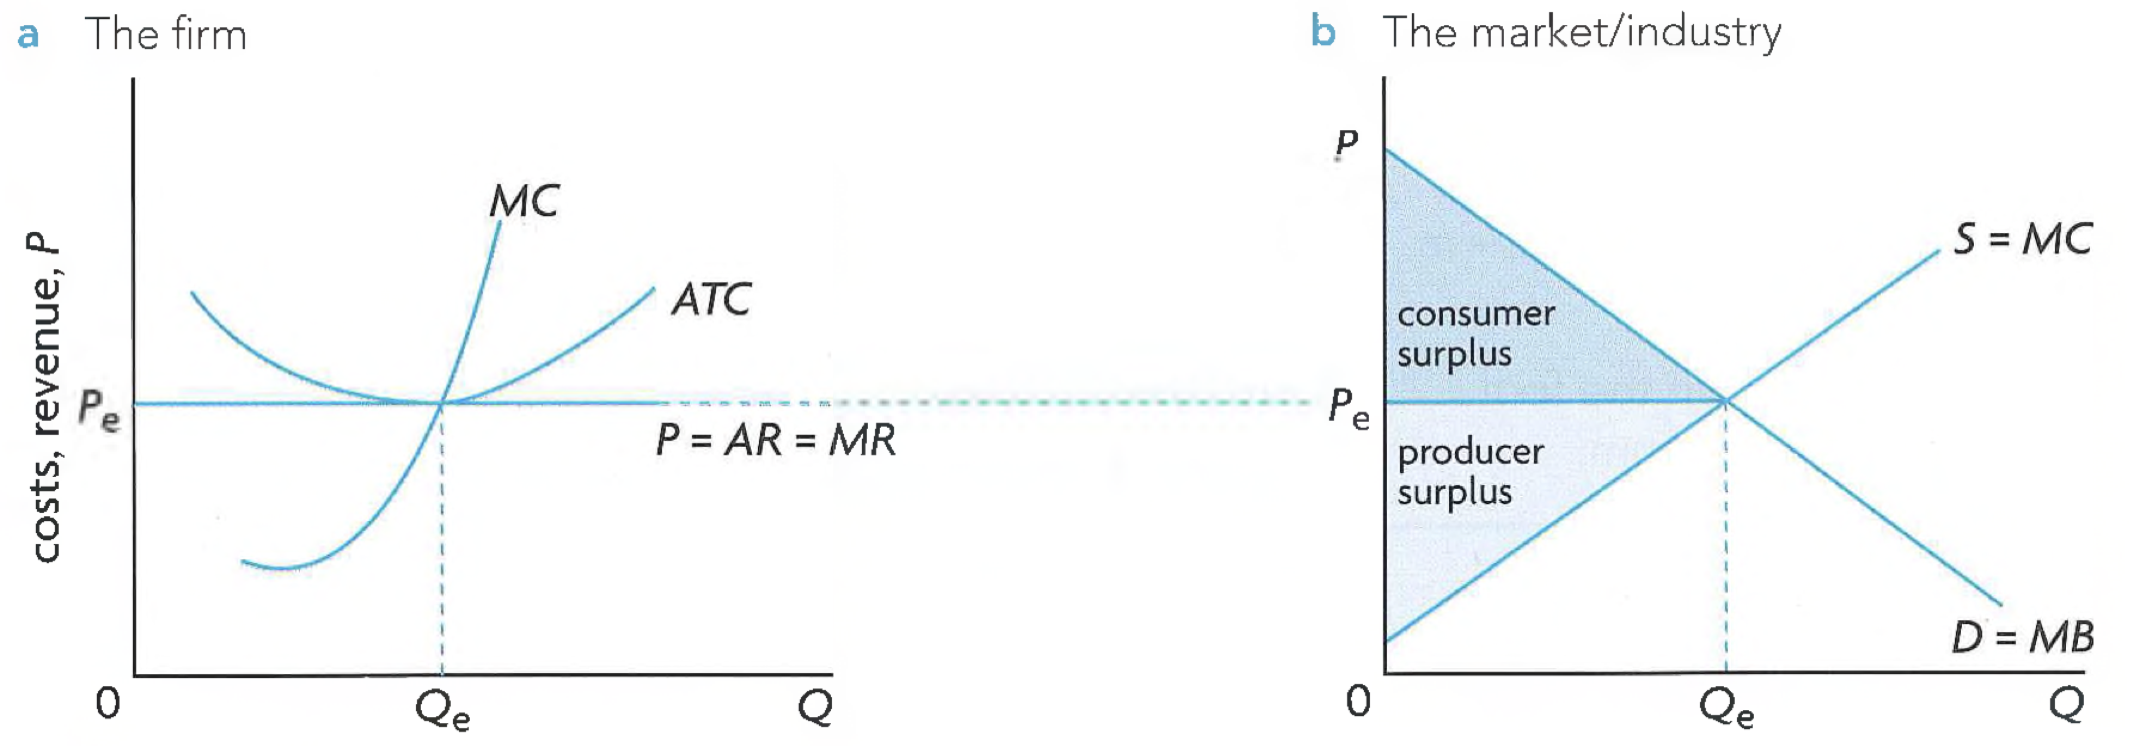
\includegraphics[width=0.8\linewidth]{Screenshot 2026-07-24 at 11.17.11.png}
\end{center}
\subsubsection*{Supplementary: Types of efficiency (Edexcel Book 2 Ch 8)}
\begin{itemize}
  \item \needbold{Productive efficiency}: production at the lowest possible average cost --- on the lowest point of the ATC curve ($P = $ minimum ATC). Achieved by perfect competition in the long run; not achieved by monopoly or monopolistic competition.
  \item \needbold{Allocative efficiency}: occurs where $P = MC$ (or $MSB = MSC$); society produces the particular mix of goods and services most wanted by consumers.
  \item \needbold{Dynamic efficiency}: efficiency over time through innovation, technological improvements, and new production processes. Typically associated with imperfectly competitive firms that have long-run abnormal profits to fund R\&D.
  \item \needbold{X-efficiency}: production with no organisational slack, keeping costs as low as possible. \textbf{X-inefficiency} occurs when lack of competitive pressure leads to organizational waste and unnecessary costs.
  \item \needbold{Social efficiency}: occurs where marginal social cost equals marginal social benefit ($MSC = MSB$), achieving the socially optimal output when externalities are taken into account.
\end{itemize}
\subsubsection*{Evaluation of the model}
\textbf{Insights (advantages):}
\begin{itemize}
  \item \textbf{Allocative efficiency}: $P = MC$ ($MB = MC$) in long-run equilibrium; social surplus is maximised.
  \item \textbf{Low prices for consumers}: absence of long-run abnormal profit keeps prices low.
  \item \textbf{Inefficient firms are driven out}: high-cost firms make losses and exit the industry in the long run.
  \item \textbf{Market responds to consumers}: demand shifts change price $\to$ short-run abnormal profits/losses $\to$ long-run adjustments in industry output.
\end{itemize}
\textbf{Limitations:}
\begin{itemize}
  \item \textbf{Unrealistic assumptions}: strict conditions rarely met in the real world.
  \item \textbf{No economies of scale}: firms are too small to grow large enough to benefit from falling average costs.
  \item \textbf{Lack of product variety}: all firms produce identical (homogeneous) goods, but consumers prefer variety.
  \item \textbf{No funds or incentive for R\&D}: zero long-run abnormal profit means no retained earnings for research; undifferentiated products remove the incentive to innovate.
\end{itemize}
\subsection{Monopoly}
\subsubsection*{Barriers to entry}
\begin{itemize}
  \item \textbf{Economies of scale}: a large firm's LRAC is substantially lower than a small firm's, so the large firm can charge a lower price and force smaller entrants out. New firms entering on a small scale cannot compete; entering on a large scale involves huge start-up costs and risk. Also significant in oligopolies.
  \item \textbf{Natural monopolies}: firms with economies of scale so large they can supply the entire market without exhausting them (see below).
  \item \textbf{Branding}: advertising creates a unique product image and \textbf{consumer loyalty}, making consumers unwilling to switch to substitutes. Limits new entrants even though it does not necessarily create a monopoly (also used in monopolistic competition and oligopoly).
  \item \textbf{Legal barriers}:
  \begin{itemize}
    \item \textbf{Patents}: government-granted exclusive right to produce a new product for a specified period (e.g.\ pharmaceuticals, microchips).
    \item \textbf{Licences}: required to operate in certain industries/professions (radio/TV, medicine, law) $\to$ limits competition.
    \item \textbf{Copyrights}: sole rights to print/publish/sell a work.
    \item \textbf{Tariffs, quotas and trade restrictions}: limit imports, reducing foreign competition.
  \end{itemize}
  \item \textbf{Control of essential resources}: monopoly arising from ownership of a key input (e.g.\ DeBeers' historical control of diamonds; Alcoa's control of bauxite). Also includes \textbf{local monopolies} --- a single supplier in a geographical area (e.g.\ a remote grocery store; sports leagues signing exclusive player/stadium contracts).
  \item \textbf{Aggressive tactics}: incumbent monopolist can deter entry by \textbf{cutting price, advertising heavily, threatening takeover}, or other dissuasive behaviour.
\end{itemize}
\subsubsection*{Demand, revenue, profit maximization}
\begin{itemize}
  \item Market power arises whenever a firm faces a downward-sloping demand curve. Firms in all market structures except perfect competition face a downward-sloping demand curve, and therefore have varying degrees of market power, or the ability to control the price at which they sell their output; they are therefore price-makers.
  \item When a firm faces a downward-sloping demand curve, price is no longer constant for all output: more output can only be sold at a lower price.
  \begin{itemize}
    \item As price falls, output increases giving rise to the downward-sloping demand curve.
    \item Marginal revenue, showing the change in total revenue resulting from a change in output, falls continuously; MR is equal to zero when total revenue is at its maximum.
    \item D = AR = P
  \end{itemize}
  \item The MR curve lies below the demand curve. 
  \item Profit-maximizing level of output determination: MC = MR
\end{itemize}
\begin{center}
  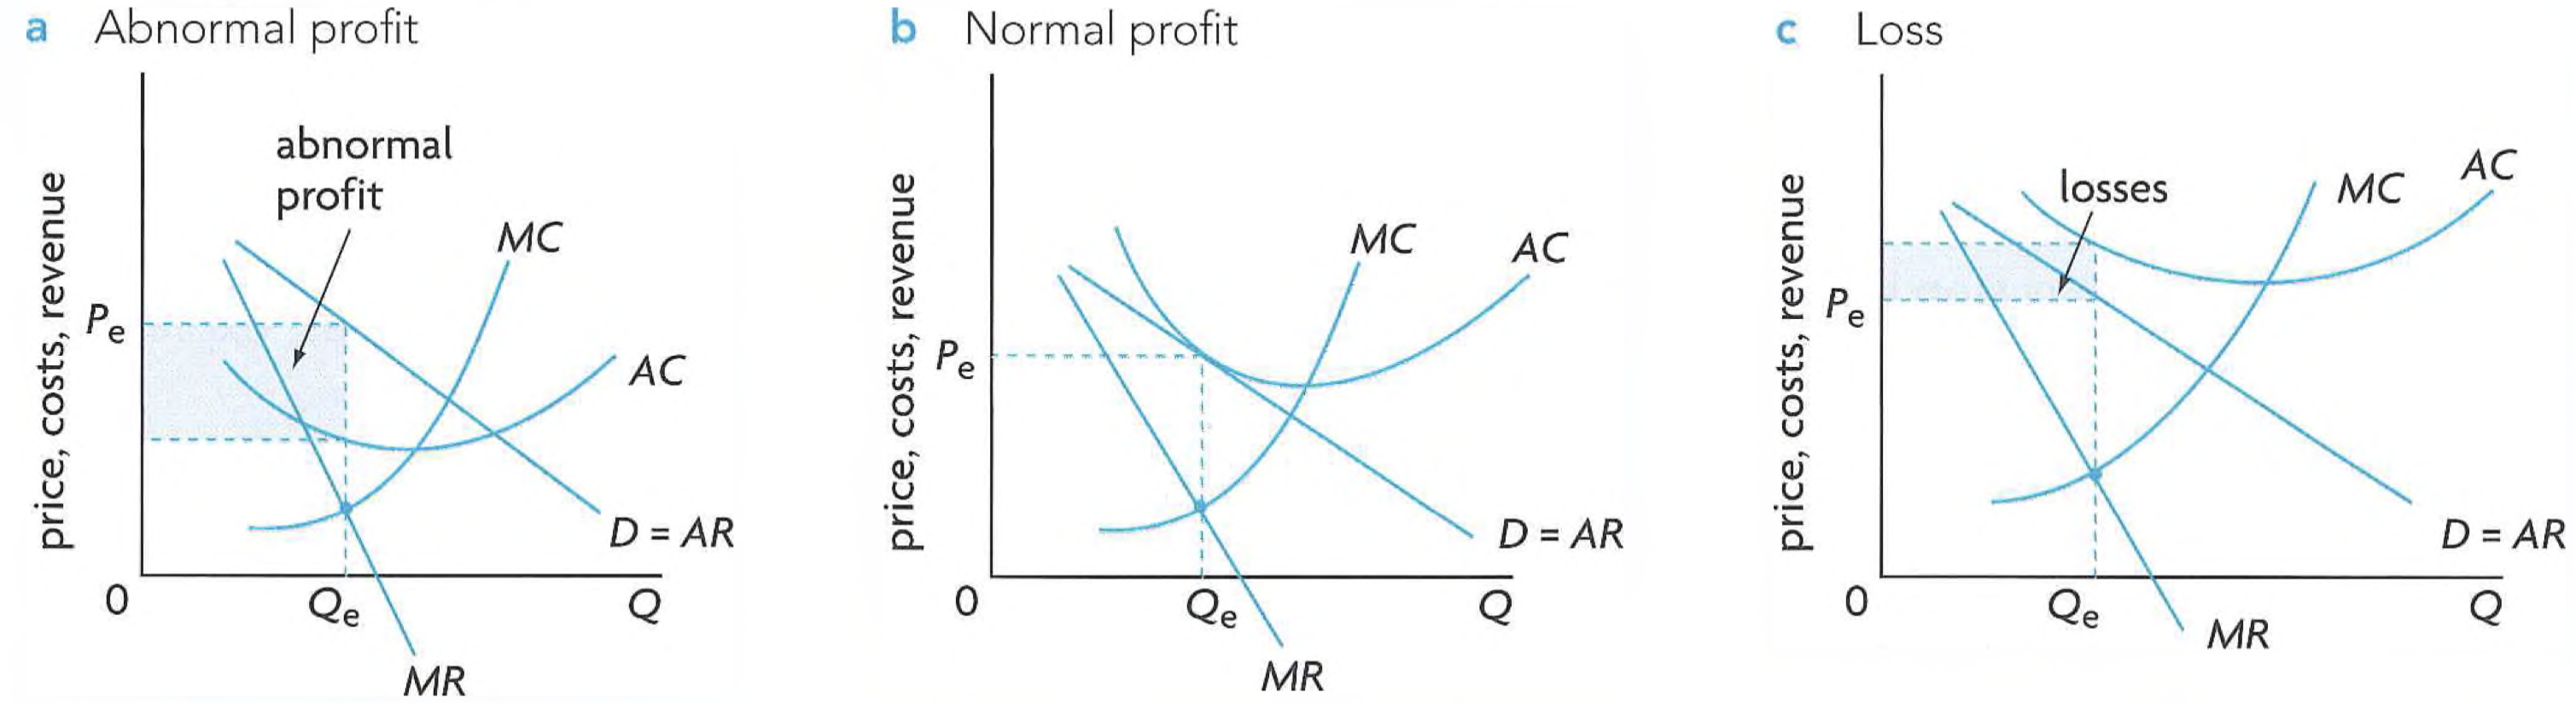
\includegraphics[width=0.99\linewidth]{Screenshot 2026-07-25 at 10.29.55.png}
\end{center}
Note that the distinction between the short run and the long run is not important in monopoly as it is in perfect competition.
\subsubsection*{Natural Monopoly}
A \needbold{natural monopoly} is a firm that has economies of scale so large that it is possible for the single firm alone to supply the entire market at a lower average cost than two or more firms.
If the market demand for a product cuts LRAC when this is falling, this means that a single large firm can produce for the entire market at a lower average total cost than two or more smaller firms. 
\begin{center}
  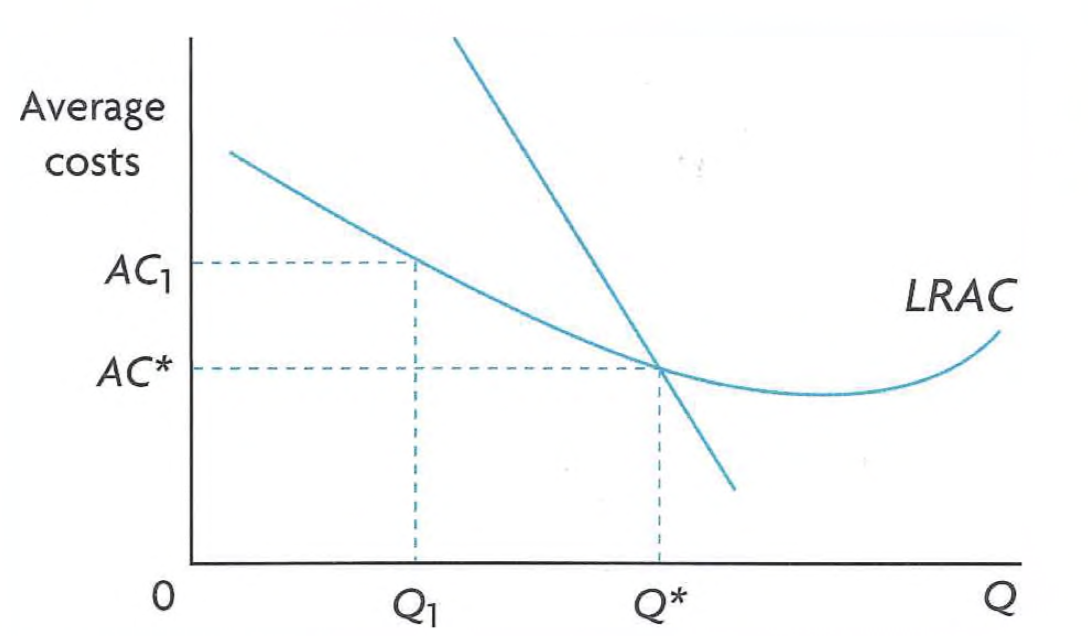
\includegraphics[width=0.4\linewidth]{Screenshot 2026-07-25 at 11.16.13.png}
\end{center}
At the level of output $Q^*$, there are still economies of scale. The figure shows that this firm cannot produce any output greater than $Q^*$ and not make a loss.\\
So if the firm is to earn normal profit or abnormal profit, it must produce a quantity less than or equal to $Q^*$ and set a price higher than $AC^*$.\\\\
A natural monopoly may stop being 'natural' if changing technologies create conditions that allow
new competitor firms to enter the industry and
begin production at a relatively low cost. 
\subsubsection*{Market outcomes and efficiency}
A comparison of monopoly with perfect competition at
the level of the industry reveals that price is higher and quantity of output produced lower in monopoly. Higher prices and lower output go against consumers' interests.
\begin{center}
  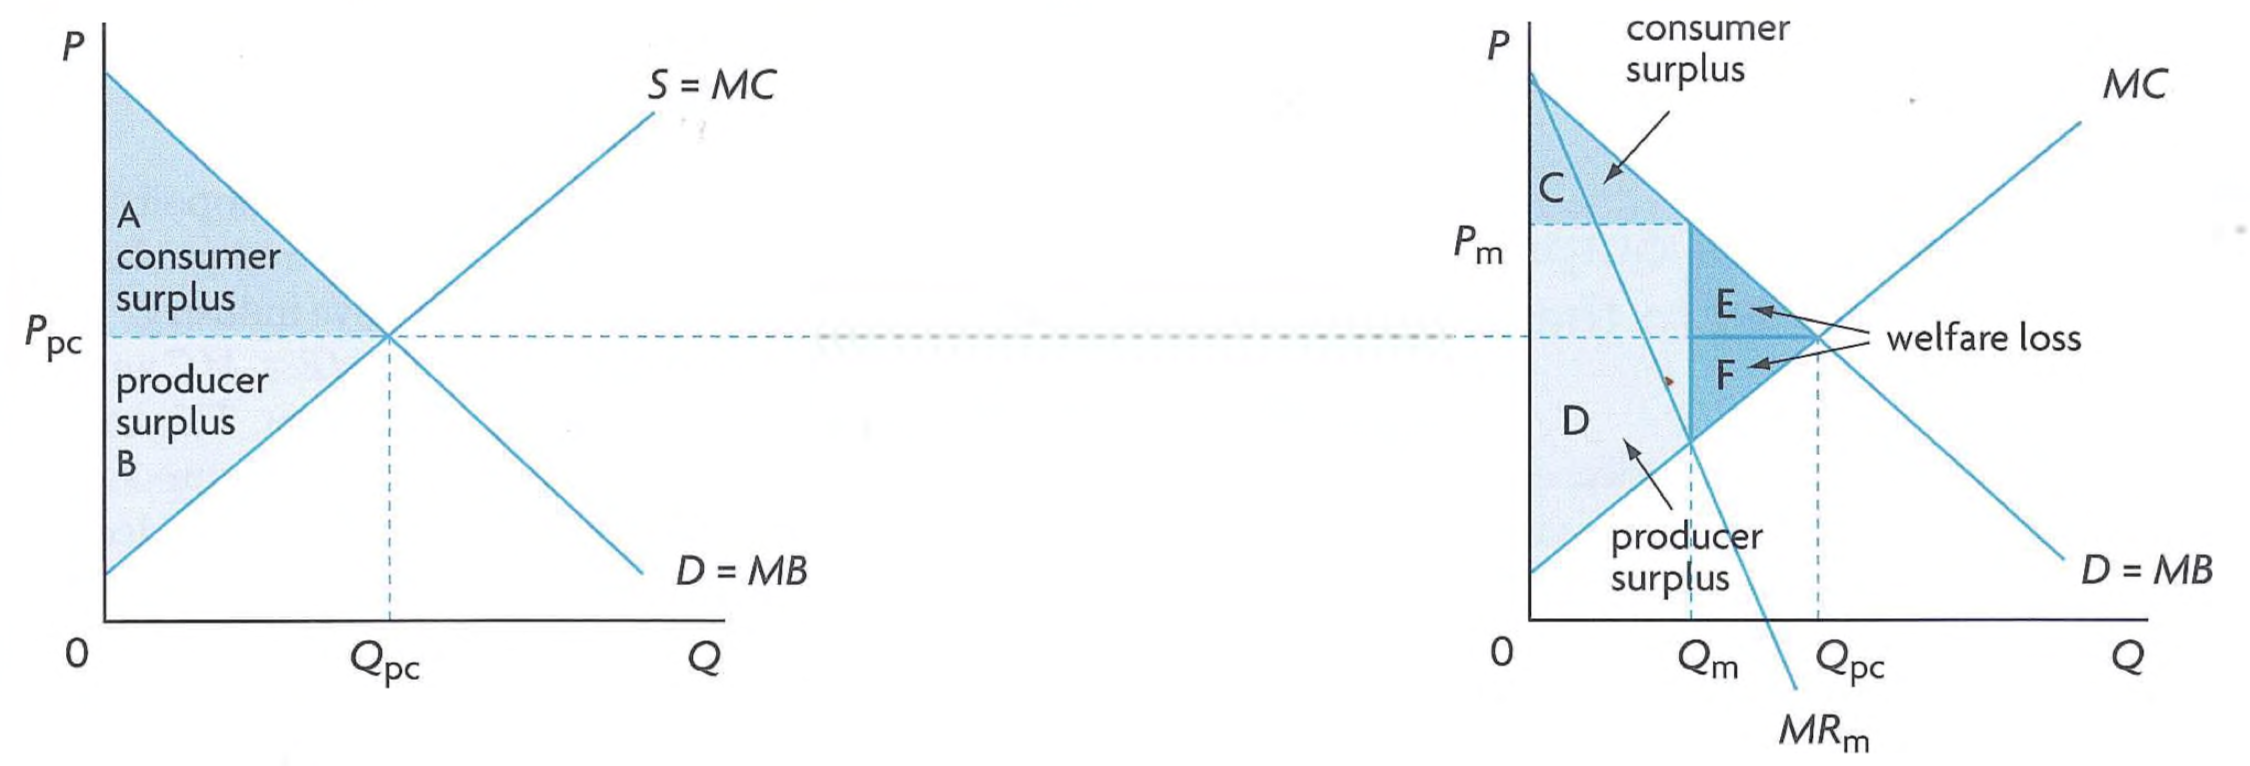
\includegraphics[width=0.8\linewidth]{Screenshot 2026-07-25 at 11.20.40.png}
\end{center}
At the point of monopoly production $Q_m$, MB > MC, meaning that it's currently underproduced (society would benefit from producing more of that good). Also, the monopolist gains at the expense of consumers as a portion of consumer surplus is converted into producer surplus.\\\\
There, at level of output $Q_m$, P > MC, meaning allocative inefficiency.\\\\
Clearly, it results in market failure (allocative inefficiency). Market power refers to the ability of a firm to charge a price greater than marginal cost, or P>MC. This can only occur when a firm faces a downward sloping demand curve.
\subsubsection*{Evaluating monopoly and comparing with perfect competition}
\textbf{Criticisms of monopoly:}
\begin{itemize}
  \item \textbf{Welfare loss \& allocative inefficiency}: $P > MC$ and $MB > MC$ at $Q_m$ $\to$ the monopolist \textbf{underallocates resources}; social surplus is reduced (market failure).
  \item \textbf{Higher price \& lower output}: compared to perfect competition, the monopolist sells \textit{less} at a \textit{higher} price $\to$ worse for consumers.
  \item \textbf{Loss of consumer surplus}: charging $P > MC$ transfers a portion of CS to the monopolist as producer surplus (monopolist gains at consumers' expense).
  \item \textbf{Negative income distribution effects}: higher prices redistribute income \textit{away from consumers} toward \textit{monopoly owners} (higher profits).
  \item \textbf{Higher costs / X-inefficiency}: lack of competitive pressure may lead to higher AC (poor motivation, lack of innovation, poor management). Long-run abnormal profits protected by barriers to entry reduce the incentive to minimise costs --- this is called \textbf{X-inefficiency}.
  \item \textbf{Possibly less innovative}: barriers to entry may shield monopolies from competition, reducing the incentive to innovate compared with firms under constant competitive pressure.
\end{itemize}
\textbf{Potential benefits of monopoly:}
\begin{itemize}
  \item \textbf{Economies of scale}: the monopolist's large size allows it to achieve \textit{lower AC} $\to$ potentially lower prices and higher output, approaching competitive levels. Society benefits from less resource waste. Perfectly competitive firms are too small to capture EOS.
  \item \textbf{Natural monopoly}: a single firm can achieve very low AC for the entire market (see natural monopolies above).
  \item \textbf{R\&D and innovation}: monopolies are better positioned to pursue R\&D because:
  \begin{itemize}
    \item \textbf{Abnormal profits} provide funds to finance R\&D projects (unavailable to perfectly competitive firms).
    \item \textbf{Barriers to entry} (including patent protection) allow the monopolist to enjoy the profits from innovation.
    \item Innovation creates \textbf{new barriers to entry} (new products rivals cannot produce), helping maintain long-run abnormal profits.
  \end{itemize}
\end{itemize}
\subsubsection*{Supplementary: Price discrimination (AP Barron Ch 8)}
\needbold{Price discrimination} is the practice of charging different prices to different consumers for the same good or service, when the price differences are \textbf{not} due to differences in the cost of production.
\\\textbf{Necessary conditions}:
\begin{itemize}
  \item The firm must possess a degree of \textbf{market power} (price-maker).
  \item The market must be separable into distinct groups with \textbf{different price elasticities of demand (PED)}. (different market segments, with differing PED)
  \item The firm must be able to \textbf{prevent resale} (arbitrage) between the markets/groups.
\end{itemize}
Firms can charge higher prices for price inelastic segments and lower prices for price elastic segments to try and maximize revenue.\\
\textbf{Degrees of price discrimination}:
\begin{itemize}
  \item \textbf{First-degree (perfect) price discrimination}: the firm charges each consumer their exact maximum willingness to pay. Consumer surplus is completely eliminated and converted into producer surplus; output expands to the competitive level where $P = MC$, eliminating deadweight loss (allocatively efficient in production, but highly unequal).
  \item \textbf{Second-degree price discrimination}: price varies according to quantity demanded or versioning (e.g.\ block pricing, quantity discounts, off-peak rates).
  \item \textbf{Third-degree price discrimination}: different prices are charged to distinct consumer groups separated by observable characteristics (e.g.\ student/senior discounts, business vs economy airline fares). The group with \textbf{more price-inelastic demand pays the higher price}.
\end{itemize}
补充：Dynamic Pricing: 根据时段、季节等外部综合因素进行定价（e.g.携程、Uber）
\subsection{Monopolistic competition}
既像Monopoly又像Perfectly competitive market的市场结构。
\subsubsection*{Product differentiation}
\begin{itemize}
  \item physical differences - products may differ in size, shape, materials, texture, taste, packaging, etc.
  \item quality differences - products can differ in quality.
  \item location - some firms attempt to differentiate their product by locating themselves in areas that allow easy access for customers, such as hotels near airports and convenience stores in residential areas.
  \item services - some firms offer specific services to make their products more attractive, such as home delivery, product demonstrations, free support, warranties and purchase terms
  \item product image - some firms attempt to create a favourable image by use of celebrity advertising or endorsements, by brand names, or attractive packaging.
\end{itemize}
It has a more elastic demand curve: it resembles perfect competition because there are many firms in the industry and there is freedom of entry. It is like monopoly because of product differentiation. ach firm in an industry is a 'mini-monopoly' in the specific version of the good that it produces. 
\\\\Monopolistically competitive firms compete with
each other on the basis of both price and non­
price competition. 
\begin{itemize}
  \item Price competition occurs when a firm lowers its price to attract customers away from rival firms, thus increasing sales at the expense of other firms.
  \item Non-price competition occurs when firms use methods other than price reductions to attract customers from rivals. (e.g., product differentiation, advertising)
\end{itemize}
\begin{center}
  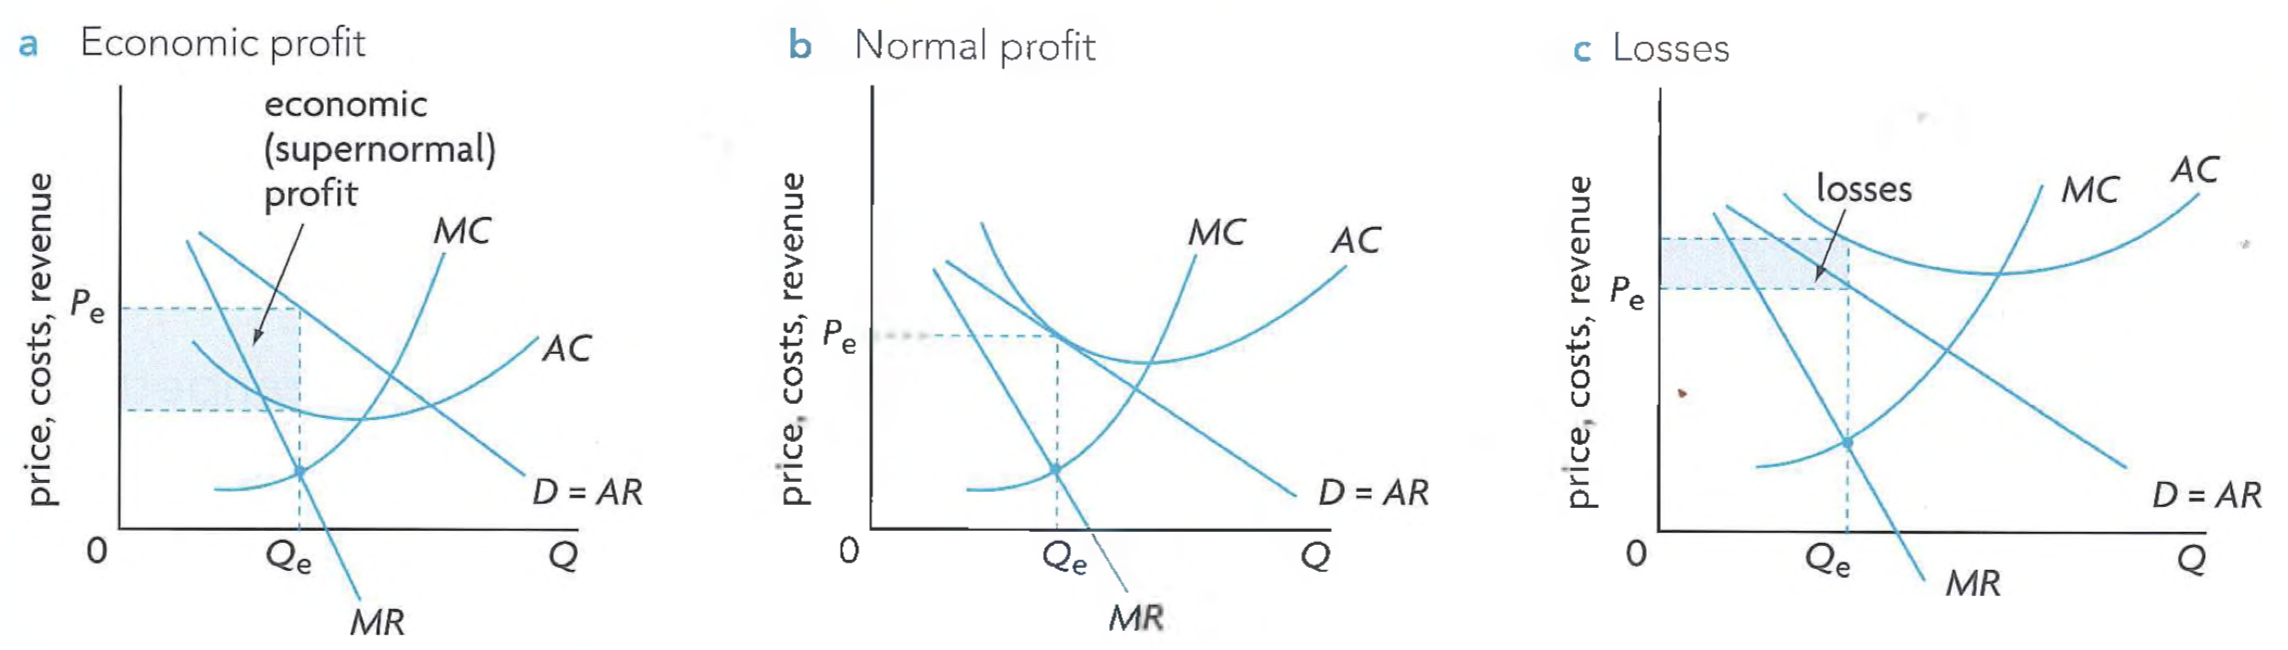
\includegraphics[width=0.95\linewidth]{Screenshot 2026-07-25 at 14.24.15.png}
\end{center}
In monopolistic competition, in the long run, profit-making industries attract new entrants; in loss-making industries, some firms shut down and exit the industry. The process of entry and exit of firms in the long run ensures that economic profit or loss is zero and all firms earn normal profit.\\\\
In monopolistic competition P>MC or alternatively MB > MC, indicating there is market failure. The market underallocates resources to the production of the good and too little of it is produced.
\subsubsection*{Supplementary: Excess capacity in monopolistic competition (AP Barron Ch 9)}
In the long-run equilibrium of monopolistic competition, free entry and exit ensure firms earn zero economic profit ($P = ATC$), but because the firm faces a downward-sloping demand curve, tangency occurs on the \textbf{downward-sloping portion of the ATC curve}:
\begin{itemize}
  \item \needbold{Excess capacity}: the firm produces an output level \textbf{below the minimum efficient scale (MES)} (the minimum of the ATC curve). The difference between the profit-maximising output and the output at minimum ATC is the excess capacity --- the industry has more firms producing smaller volumes than would minimise average cost.
  \item \needbold{Markup over marginal cost}: because demand is downward-sloping, $P > MR = MC$. The price markup reflects market power, meaning allocative efficiency is not achieved ($P > MC$).
\end{itemize}
\subsubsection*{Comparison with other market structures}
\textbf{Monopolistic competition vs.\ perfect competition --- similarities:}
\begin{itemize}
  \item Large number of firms; free entry (no barriers).
  \item Normal profit in the long run; abnormal profit or loss only in the short run.
\end{itemize}
\textbf{Differences:}
\begin{itemize}
  \item \textbf{Market power}: PC firms have none (horizontal $D$, price-takers); MC firms have some (downward-sloping $D$).
  \item \textbf{Allocative efficiency}: PC achieves it ($P = MC$); MC does not ($P > MC$) $\to$ market failure.
  \item \textbf{Product variety}: PC offers none (homogeneous goods); MC offers differentiation --- an advantage for consumers, though some inefficiency is the ``price'' paid for variety.
  \item \textbf{Economies of scale}: PC firms are too small; MC firms may achieve only small EOS.
\end{itemize}
\textbf{Monopolistic competition vs.\ monopoly --- similarities:}
\begin{itemize}
  \item Both face downward-sloping $D$ with $MR$ below it $\to$ $P > MC$ at the profit-maximising output $\to$ neither achieves allocative efficiency (both are forms of market failure).
\end{itemize}
\textbf{Differences:}
\begin{itemize}
  \item \textbf{Number \& size of firms}: MC has many small firms; monopoly has one large (or dominant) firm.
  \item \textbf{Barriers to entry}: MC has free entry; monopoly has high barriers.
  \item \textbf{Profits}: MC earns only normal profit in the long run; monopoly can maintain \textbf{abnormal profits} long run (due to barriers).
  \item \textbf{Prices \& output}: MC has lower prices and higher output than monopoly (free entry drives profits to zero) $\to$ more consumer-friendly.
  \item \textbf{Market power}: monopoly has more (no close substitutes); MC firms have less (consumers can switch to substitutes).
  \item \textbf{Costs}: competition in MC puts downward pressure on costs and drives out inefficient firms; monopoly lacks this pressure (risk of X-inefficiency).
  \item \textbf{R\&D}: monopoly is better funded (abnormal profits) for large R\&D; MC firms face competitive pressure to innovate for product development.
  \item \textbf{EOS / natural monopoly}: monopoly has far greater EOS potential; possible natural monopoly.
  \item \textbf{Product variety}: MC offers greater variety (many differentiated substitutes); monopoly typically offers less.
\end{itemize}
\subsection{Oligopoly}
\subsubsection*{Interdependence and game theory}
Implications for their behavior:
\begin{itemize}
  \item Strategic behavior: based on plans of action that take into account rivals' possible courses of action. (Like CHESS) 
  \item Conflicting incentives. Firms in oligopoly face incentives that conflict, or clash with each other:
  \begin{itemize}
    \item Incentive to collude: an agreement between firms to limit competition between them, usually by fixing price and therefore lowering quantity produced. This reduces uncertainty and maximize profits for the whole industry.
    \item Incentive to compete / cheat: each firm faces an incentive to compete with its rivals in the hope that it will capture a portion of its rivals’ market shares and profits, thereby increasing profits at the expense of other firms. 
  \end{itemize}
\end{itemize}
\subsubsection*{Oligopoly payoff matrix}
The game we will use here illustrates the prisoner's dilemma, showing how two rational decision-makers, who use strategic behaviour to maximise profits by
trying to guess the rival's behaviour, may end up being collectively worse off. The final position that results from the game is called a Nash equilibrium.\\\\
The Nash equilibrium shows that there is sometimes a conflict between the pursuit of individual self-interest and the collective firm interest. This conflict is the prisoner's dilemma. Although the firms could be better off by cooperating, each firm, trying to make itself better off, ends up making both itself and its rival worse off.
\\\\\textbf{How to read the matrix}: each cell shows the profit for Firm A (left) and Firm B (right) given their simultaneous choices.
\begin{itemize}
  \item If both charge a \textbf{high price} (collude), each earns \textbf{50} --- the best \textit{joint} outcome.
  \item If A \textbf{cheats} (low price) while B keeps high price, A captures market share: A earns \textbf{80}, B only \textbf{20}. Symmetrically for B cheating.
  \item If \textbf{both cheat} (both charge low price), each earns only \textbf{30} --- worse than if they had both kept high prices.
\end{itemize}
\begin{center}
\renewcommand{\arraystretch}{1.8}
\begin{tabular}{cc|c|c|}
  & \multicolumn{1}{c}{} & \multicolumn{2}{c}{\textbf{Firm B}} \\
  & \multicolumn{1}{c}{} & \textbf{High price} & \textbf{Low price} \\
  \cline{3-4}
\parbox[t]{2cm}{\centering\textbf{Firm A}} & \textbf{High price} & \makecell[cc]{$A$: 50\\$B$: 50} & \makecell[cc]{$A$: 20\\$B$: 80} \\
  \cline{3-4}
  & \textbf{Low price} & \makecell[cc]{$A$: 80\\$B$: 20} & \makecell[cc]{$A$: 30\\$B$: 30} \\
  \cline{3-4}
\end{tabular}
\end{center}
This game illustrates many real-world aspects of oligopolistic firms, which:
\begin{itemize}
  \item are independent
  \item display strategic behavior
  \item facing conflicting incentives
  \item become worse off as a result of price competition (price war)
  \item have a strong interest in avoiding price wars, because they realise that every one will become worse off through price cutting
\end{itemize}
\subsubsection*{Supplementary: Game theory concepts --- Dominant strategy and Nash equilibrium (AP Barron Ch 9)}
\begin{itemize}
  \item \needbold{Dominant strategy}: a strategy that yields the highest payoff for a player \textbf{regardless} of what the rival does.
  \item \needbold{Nash equilibrium}: a set of strategies where \textbf{no player can improve their payoff by unilaterally changing} their own strategy, given the rival's strategy. (In the prisoner's dilemma matrix above, each firm's dominant strategy is to choose the low price, making both choosing low price the Nash equilibrium even though both would prefer mutual cooperation.)
\end{itemize}
Common methods of non-price competition:
\begin{itemize}
  \item R\&D
  \item Advertising
  \item Branding
  \item numerous services like quality customer service, warranties, provision of credit, discounts on upgrades and others.
\end{itemize}
They are important because:
\begin{itemize}
  \item Oligopolistic firms often have considerable financial resources.
  \item The development of new products provides firms with a competitive edge, increase market power, have a less elastic demand curve
  \item Product differentiation can increase a firm's profit without creating risks for immediate retaliation by rivals.
\end{itemize}
Two types of oligopoly:
\begin{itemize}
  \item Collusive oligopoly: firms agree to collude, which means they form an agreement between themselves to limit competition, increase market power and increase profit. (e.g. setting a fixed price, limit the amount of price difference)
  \begin{itemize}
    \item Cartel: formal agreement between firms in an industry to take actions to limit competition in order to increase profits. Cartel members collectively behave like a monopoly.
    \item Benefits of Cartel:
    \begin{itemize}
      \item increased market power and hence the ability to control price of the product
      \item increased profits due to higher prices
      \item elimination of competition between the firms, and therefore no more uncertainty or need to outguess their rivals.
    \end{itemize}
    \item However, it's not easy to maintain due to:
    \begin{itemize}
      \item The incentive to cheat
      \item Cost differences between firms
      \item Number of firms
      \item The possibility of a price war
    \end{itemize}
    \item Other types of collusive oligopoly: informal collusion (no formal agreement) (including price leadership, in which the dominant firm sets a price and also initiates any price changes)
  \end{itemize}
  \item Non-collusive oligopoly: oligopolistic firms that do not collude in any way in order to fix or coordinate prices and limit competition. Each firm behaves independently.
  \begin{itemize}
    \item Firms that do not collude are forced to take into account the actions of their rivals in making pricing decisions.
    \item Even though the firms do not collude, there is still price stability.
    \item Firms do not compete with each other on the basis of price.
  \end{itemize}
\end{itemize}
A \needbold{concentration ratio} provides an indication of the percentage of output produced by the largest firms in an industry; it measures market concentration.
Concentration ratios provide an indication of the degree of competition in an industry. In general, an industry is considered to be oligopolistic if the four largest firms control 40\% (arbitrary) of output.\\
Weaknesses of concentration ratio as a method of determining market concentration:
\begin{itemize}
  \item Whereas concentration ratios reflect concentration in a national market, they do not reflect competition from abroad, arising from imports.
  \item Concentration ratios provide no indication of the importance of firms in the global market.
  \item Concentration ratios do not account for competition from other industries, which maybe important in the case of substitute goods.
  \item Concentration ratios do not distinguish between different possible sizes of the largest firms.
\end{itemize}
\subsubsection*{Evaluation of oligopoly}
\textbf{Criticisms} (similar to monopoly):
\begin{itemize}
  \item \textbf{Welfare loss, allocative inefficiency \& market failure}: $P > MC$, underallocation of resources.
  \item \textbf{Higher prices \& lower output} than under competitive conditions.
  \item \textbf{Loss of consumer surplus} transferred to oligopolists via higher prices.
  \item \textbf{Negative income distribution effects}: profits shift from consumers to oligopoly owners.
  \item \textbf{Possibly higher costs} due to lack of price competition (X-inefficiency).
  \item \textbf{Possibly less innovative}.
  \item \textbf{Collusion risk}: even with anti-monopoly legislation, collusion among oligopolists is hard to detect and prove --- firms may behave like monopolies yet escape regulation.
\end{itemize}
\textbf{Benefits} (similar to monopoly):
\begin{itemize}
  \item \textbf{Economies of scale}: large firm size $\to$ lower AC $\to$ potentially lower prices for consumers and less resource waste.
  \item \textbf{R\&D and innovation}: abnormal profits fund large research projects; non-price competition forces firms to innovate to maintain/gain market share (even more so than in monopoly).
  \item \textbf{Lower prices from efficiency gains}: technological improvements may be passed on to consumers.
  \item \textbf{Greater product variety}: product development leads to increased differentiation and consumer choice (an advantage over monopoly, which offers little variety).
\end{itemize}
\subsubsection*{Supplementary: Contestable markets (Edexcel Book 2 Ch 13--14)}
\needbold{Contestable market}: a market where entry and exit are very easy because \textbf{sunk costs are low}, even if only few firms currently operate. Potential competition (``hit-and-run'' entry) forces existing firms to behave efficiently, eliminate X-inefficiency, and keep prices near average cost, even without many actual rivals.
\subsection{Government intervention in response to abuse of market power}
Abuse of market power: firms engage in activities that result in reduced competition. Examples include:
\begin{itemize}
  \item charging unreasonably high prices
  \item depriving smaller competitors of customers by selling at artificially low prices they can't compete with
  \item obstructing competitors in the market (or in another related market) by forcing consumers to buy a product which is artificially related to a more popular, in-demand product
  \item refusing to deal with certain customers or offering special discounts to customers who buy all or most of their supplies from the dominant company
  \item making the sale of one product conditional on the sale of another product
\end{itemize}
\subsubsection*{Legislation to protect competition (competition policy)}
Most countries have laws to \textbf{prevent collusion} among oligopolists and \textbf{anti-competitive behaviour} by dominant firms. Firms found guilty face \textbf{fines} or may be \textbf{broken up} into smaller firms. Difficulties:
\begin{itemize}
  \item \textbf{Interpretation}: laws may be vague; distinguishing abuse of market power from legitimate action is highly controversial.
  \item \textbf{Enforcement varies} by government priorities/ideology --- some believe strict intervention is needed; others believe market forces self-correct over time (a normative issue).
  \item \textbf{Collusion is secret} and hard to discover/prove.
\end{itemize}
\textbf{Mergers}: a merger is an agreement by two or more firms to combine into one. Mergers may pursue EOS, growth, or market power. Competition policy limits mergers that would create too much market power. \textit{Difficulties}: uncertainties over which mergers to allow; ideological differences on acceptable market power.
\\
\textbf{Fines}: firms may calculate that profits from illegal behaviour exceed the fine (especially if they might not get caught). Big firms may ignore ethics if non-compliance is more profitable than compliance.
\subsubsection*{Regulation of natural monopolies}
Natural monopolies are not broken up (doing so would raise AC and waste resources). Two main regulatory approaches:
\begin{itemize}
  \item \textbf{Marginal cost pricing} ($P = MC$): achieves \textbf{allocative efficiency} (lowest $P$, highest $Q$). However, for a natural monopolist $P = MC < AC$, so the firm makes \textbf{losses} $\to$ requires government subsidy or the firm shuts down. Not a popular method.
  \item \textbf{Average cost pricing} ($P = AC$): the firm earns \textbf{normal profit} (no loss, no shutdown). Results in higher $P$ and lower $Q$ than marginal cost pricing, but still \textbf{better than the unregulated monopoly outcome}. Allocative efficiency is \textit{not} achieved but welfare loss is reduced.\\
  \textit{Disadvantages}: removes the incentive to keep costs low (if costs rise, the regulated price rises too); the firm may continue to be protected even if it is no longer a natural monopoly due to technological change (e.g.\ telecommunications).
\end{itemize}
\begin{center}
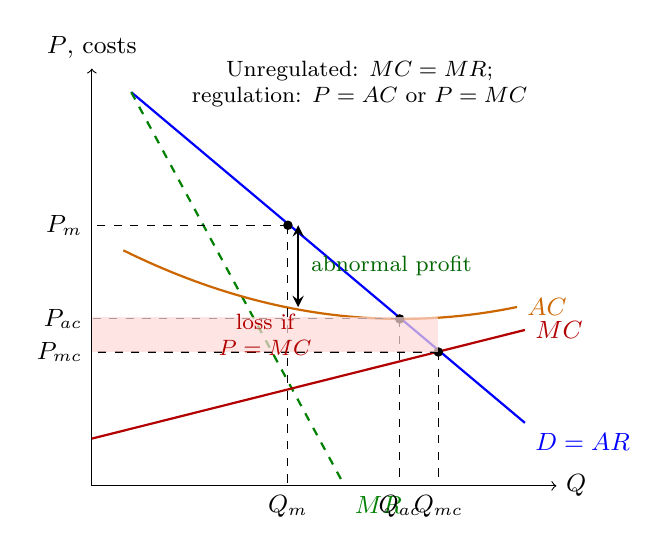
\begin{tikzpicture}[scale=1.0]
\draw[->] (0,0) -- (5.9,0) node[right, font=\small] {$Q$};
\draw[->] (0,0) -- (0,5.3) node[above, font=\small] {$P$, costs};
% D, MR, MC, AC
\draw[thick, blue] (0.5,5.0) -- (5.5,0.8) node[below right, blue, font=\small] {$D = AR$};
\draw[thick, green!50!black, dashed] (0.5,5.0) -- (3.21,0) node[below right, green!50!black, font=\small] {$MR$};
\draw[thick, red!70!black] (0,0.6) -- (5.5,1.98) node[right, red!70!black, font=\small] {$MC$};
\draw[thick, orange!80!black] plot[domain=0.4:5.4, samples=50] (\x, {3.2-0.55*\x+0.07*\x^2}) node[right, orange!80!black, font=\small] {$AC$};
% Unregulated monopoly: MR = MC
\filldraw (2.49,3.31) circle (1.5pt);
\draw[dashed] (2.49,3.31) -- (2.49,0) node[below, font=\small] {$Q_m$};
\draw[dashed] (2.49,3.31) -- (0,3.31) node[left, font=\small] {$P_m$};
% Average cost pricing: D = AC
\filldraw (3.91,2.12) circle (1.5pt);
\draw[dashed] (3.91,2.12) -- (3.91,0) node[below, font=\small] {$Q_{ac}$};
\draw[dashed] (3.91,2.12) -- (0,2.12) node[left, font=\small] {$P_{ac}$};
% Marginal cost pricing: D = MC
\filldraw (4.40,1.70) circle (1.5pt);
\draw[dashed] (4.40,1.70) -- (4.40,0) node[below, font=\small] {$Q_{mc}$};
\draw[dashed] (4.40,1.70) -- (0,1.70) node[left, font=\small] {$P_{mc}$};
% Loss rectangle at MC pricing
\fill[red!15, opacity=0.7] (0,1.70) rectangle (4.40,2.14);
\node[font=\footnotesize, red!70!black, align=center] at (2.2,1.92) {loss if\\$P = MC$};
% Abnormal profit at unregulated Qm (AC at Qm = 2.27)
\draw[<->, >=stealth, thick] (2.62,2.27) -- (2.62,3.31);
\node[font=\footnotesize, green!40!black, right] at (2.66,2.79) {abnormal profit};
\node[font=\footnotesize, align=center] at (3.4,5.1) {Unregulated: $MC=MR$;\\ regulation: $P=AC$ or $P=MC$};
\end{tikzpicture}
\end{center}
\textbf{Government ownership}: an alternative where the government owns the natural monopoly and can force lower prices / higher output. \textit{Disadvantage}: government firms lack profit-maximising incentives $\to$ inefficiency and higher costs. Global trend since the 1990s has been toward \textbf{privatization}.

\subsection{Supplementary: Factor (resource) markets and monopsony (AP Barron Ch 10 \& Edexcel Book 2 Ch 13--14)}
In factor (resource) markets, firms are the \textbf{buyers} of factors of production (such as labour, capital, and land) and households are the \textbf{sellers}.
\begin{itemize}
  \item \needbold{Derived demand}: demand for a factor of production is not demanded for its own sake, but is \textbf{derived} from the demand for the final goods and services it helps produce.
  \item \needbold{Marginal revenue product (MRP)}: the additional revenue generated by employing one more unit of an input:
  \[MRP = MP \times P \qquad \text{or} \qquad MRP = \dfrac{\Delta TR}{\Delta L}\]
  Because of the law of diminishing returns, $MP$ eventually falls, making the $MRP$ curve downward-sloping. The $MRP$ curve represents the firm's \textbf{demand curve for labour}.
  \item \needbold{Marginal factor cost (MFC)}: the additional cost incurred by employing one more unit of an input:
  \[MFC = \dfrac{\Delta TC}{\Delta L}\]
  \item \textbf{Profit-maximising hiring rule}: a firm hires labour up to the point where:
  \[MRP = MFC\]
  \item In a \textbf{perfectly competitive labour market}, each individual firm is a \textbf{wage taker} facing a horizontal labour supply curve at market wage $W$. Therefore $MFC = W$, and the firm hires where $MRP = W$.
  \item \textbf{Least-cost rule} for two inputs (labour $L$ and capital $K$):
  \[\dfrac{MP_L}{P_L} = \dfrac{MP_K}{P_K}\]
  To maximise total profits, the firm also ensures that:
  \[\dfrac{MRP_L}{P_L} = \dfrac{MRP_K}{P_K} = 1\]
\end{itemize}

\textbf{Perfectly competitive labour market} (many firms hiring workers with similar skills; each firm is a \textbf{wage taker}):
\begin{center}
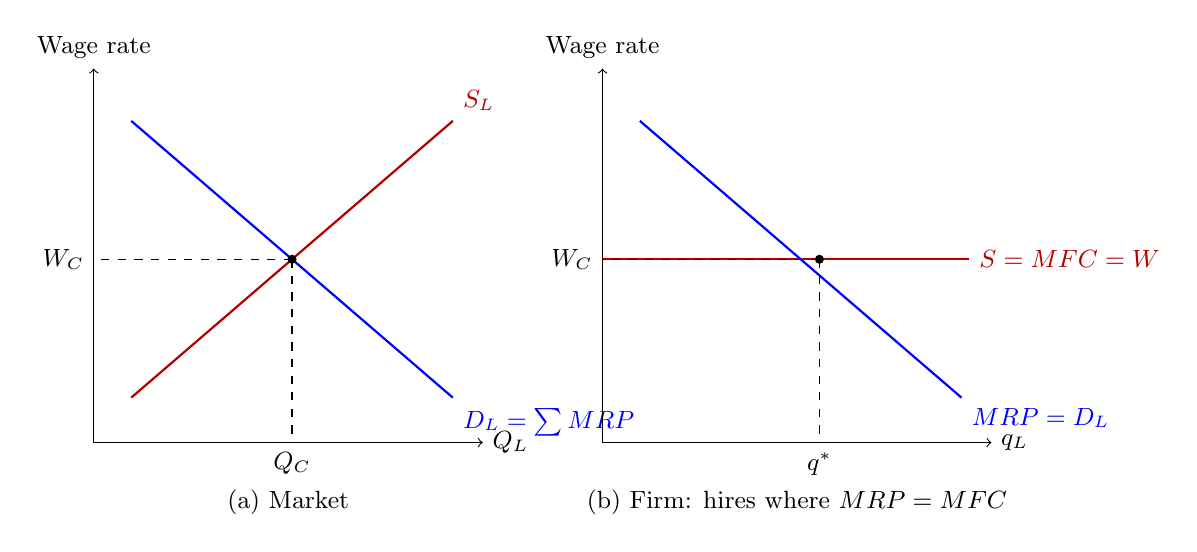
\begin{tikzpicture}[scale=0.95]
% --- Market ---
\begin{scope}
\draw[->] (0,0) -- (5.2,0) node[right, font=\small] {$Q_L$};
\draw[->] (0,0) -- (0,5.0) node[above, font=\small] {Wage rate};
\draw[thick, red!70!black] (0.5,0.6) -- (4.8,4.3) node[above right, red!70!black, font=\small] {$S_L$};
\draw[thick, blue] (0.5,4.3) -- (4.8,0.6) node[below right, blue, font=\small] {$D_L = \sum MRP$};
\filldraw (2.65,2.45) circle (1.5pt);
\draw[dashed] (2.65,2.45) -- (2.65,0) node[below, font=\small] {$Q_C$};
\draw[dashed] (2.65,2.45) -- (0,2.45) node[left, font=\small] {$W_C$};
\node[font=\small, align=center] at (2.6,-0.8) {(a) Market};
\end{scope}
% --- Firm ---
\begin{scope}[xshift=6.8cm]
\draw[->] (0,0) -- (5.2,0) node[right, font=\small] {$q_L$};
\draw[->] (0,0) -- (0,5.0) node[above, font=\small] {Wage rate};
\draw[thick, red!70!black] (0,2.45) -- (4.9,2.45) node[right, red!70!black, font=\small] {$S = MFC = W$};
\draw[thick, blue] (0.5,4.3) -- (4.8,0.6) node[below right, blue, font=\small] {$MRP = D_L$};
\filldraw (2.9,2.45) circle (1.5pt);
\draw[dashed] (2.9,2.45) -- (2.9,0) node[below, font=\small] {$q^*$};
\draw[dashed] (2.9,2.45) -- (0,2.45) node[left, font=\small] {$W_C$};
\node[font=\small, align=center] at (2.6,-0.8) {(b) Firm: hires where $MRP = MFC$};
\end{scope}
\end{tikzpicture}
\end{center}

\textbf{Monopsony} (single buyer of labour, e.g.\ the sole dominant employer in a town or an industry buyer):
\begin{itemize}
  \item Because the monopsonist faces the entire \textbf{upward-sloping market supply of labour}, hiring an additional worker requires paying a higher wage not only to the marginal worker but to \textbf{all previously hired workers}.
  \item Consequently, the marginal factor cost lies strictly \textbf{above} the labour supply curve: $MFC > W$.
  \item The monopsonist profit-maximises by hiring where $MFC = MRP$ (quantity $Q_M$), but pays the lower wage $W_M$ determined by the supply curve at $Q_M$.
  \item Outcome: the monopsonist hires \textbf{fewer workers at a lower wage} ($Q_M < Q_C$ and $W_M < W_C$) compared to a competitive market, creating deadweight loss and market failure.
  \item \textbf{Policy remedy}: setting a \textbf{minimum wage} between $W_M$ and $W_C$ makes the labour supply curve horizontal up to that minimum wage, eliminating the upward-sloping $MFC$ penalty. Under monopsony, a minimum wage can therefore \textbf{increase both wages and employment} toward the competitive level.
\end{itemize}
\begin{center}
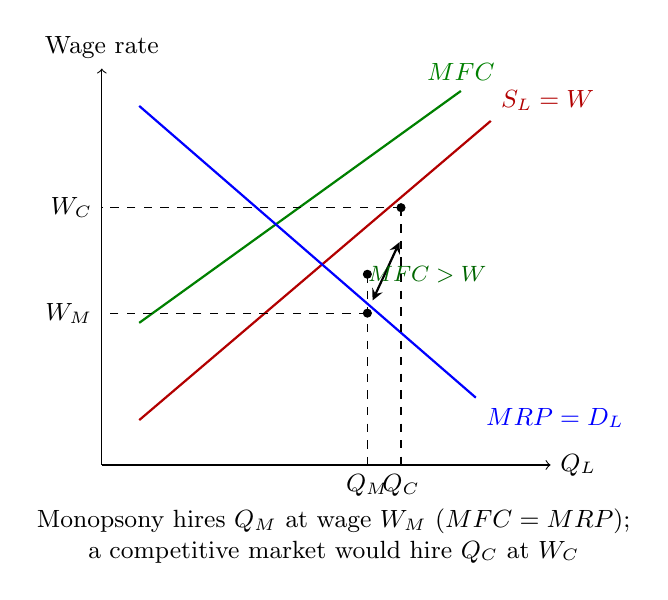
\begin{tikzpicture}[scale=0.95]
\draw[->] (0,0) -- (6.0,0) node[right, font=\small] {$Q_L$};
\draw[->] (0,0) -- (0,5.3) node[above, font=\small] {Wage rate};
% Supply and MFC (upward-sloping, MFC steeper)
\draw[thick, red!70!black] (0.5,0.6) -- (5.2,4.6) node[above right, red!70!black, font=\small] {$S_L = W$};
\draw[thick, green!50!black] (0.5,1.9) -- (4.8,5.0) node[above, green!50!black, font=\small] {$MFC$};
% MRP
\draw[thick, blue] (0.5,4.8) -- (5.0,0.9) node[below right, blue, font=\small] {$MRP = D_L$};
% Monopsony equilibrium: MFC = MRP
\filldraw (3.55,2.55) circle (1.5pt);
\draw[dashed] (3.55,2.55) -- (3.55,0) node[below, font=\small] {$Q_M$};
% Wage from supply at QM
\draw[dashed] (3.55,2.55) -- (3.55,2.03);
\filldraw (3.55,2.03) circle (1.5pt);
\draw[dashed] (3.55,2.03) -- (0,2.03) node[left, font=\small] {$W_M$};
% Competitive equilibrium: S = MRP
\filldraw (4.0,3.44) circle (1.5pt);
\draw[dashed] (4.0,3.44) -- (4.0,0) node[below, font=\small] {$Q_C$};
\draw[dashed] (4.0,3.44) -- (0,3.44) node[left, font=\small] {$W_C$};
\draw[<->, >=stealth, thick] (3.62,2.20) -- (3.98,2.98);
\node[font=\footnotesize, green!40!black] at (4.35,2.55) {$MFC > W$};
\node[font=\small, align=center] at (3.1,-0.95) {Monopsony hires $Q_M$ at wage $W_M$ ($MFC = MRP$);\\ a competitive market would hire $Q_C$ at $W_C$};
\end{tikzpicture}
\end{center}
\newpage
% ------------------------------------------------------------
\section*{Unit 3 Macroeconomics}
\section{The level of overall economic activity}
\subsection{Economic activity}
忘了就去复习Chapter 1.3.
\begin{center}
  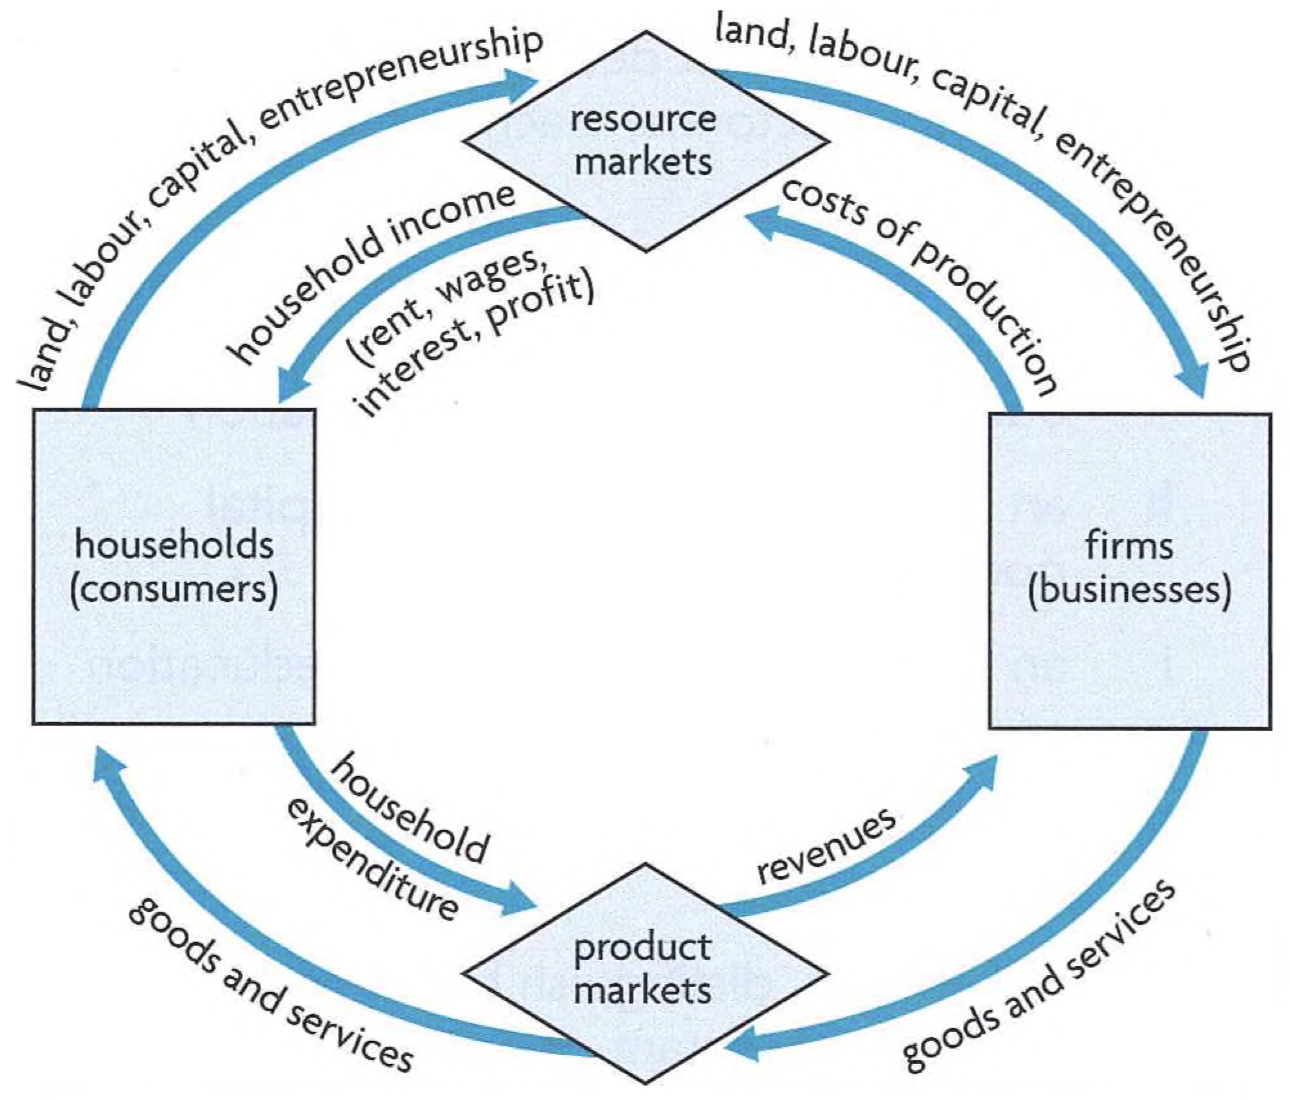
\includegraphics[width=0.36\linewidth]{Screenshot 2026-07-14 at 10.28.33.png}
  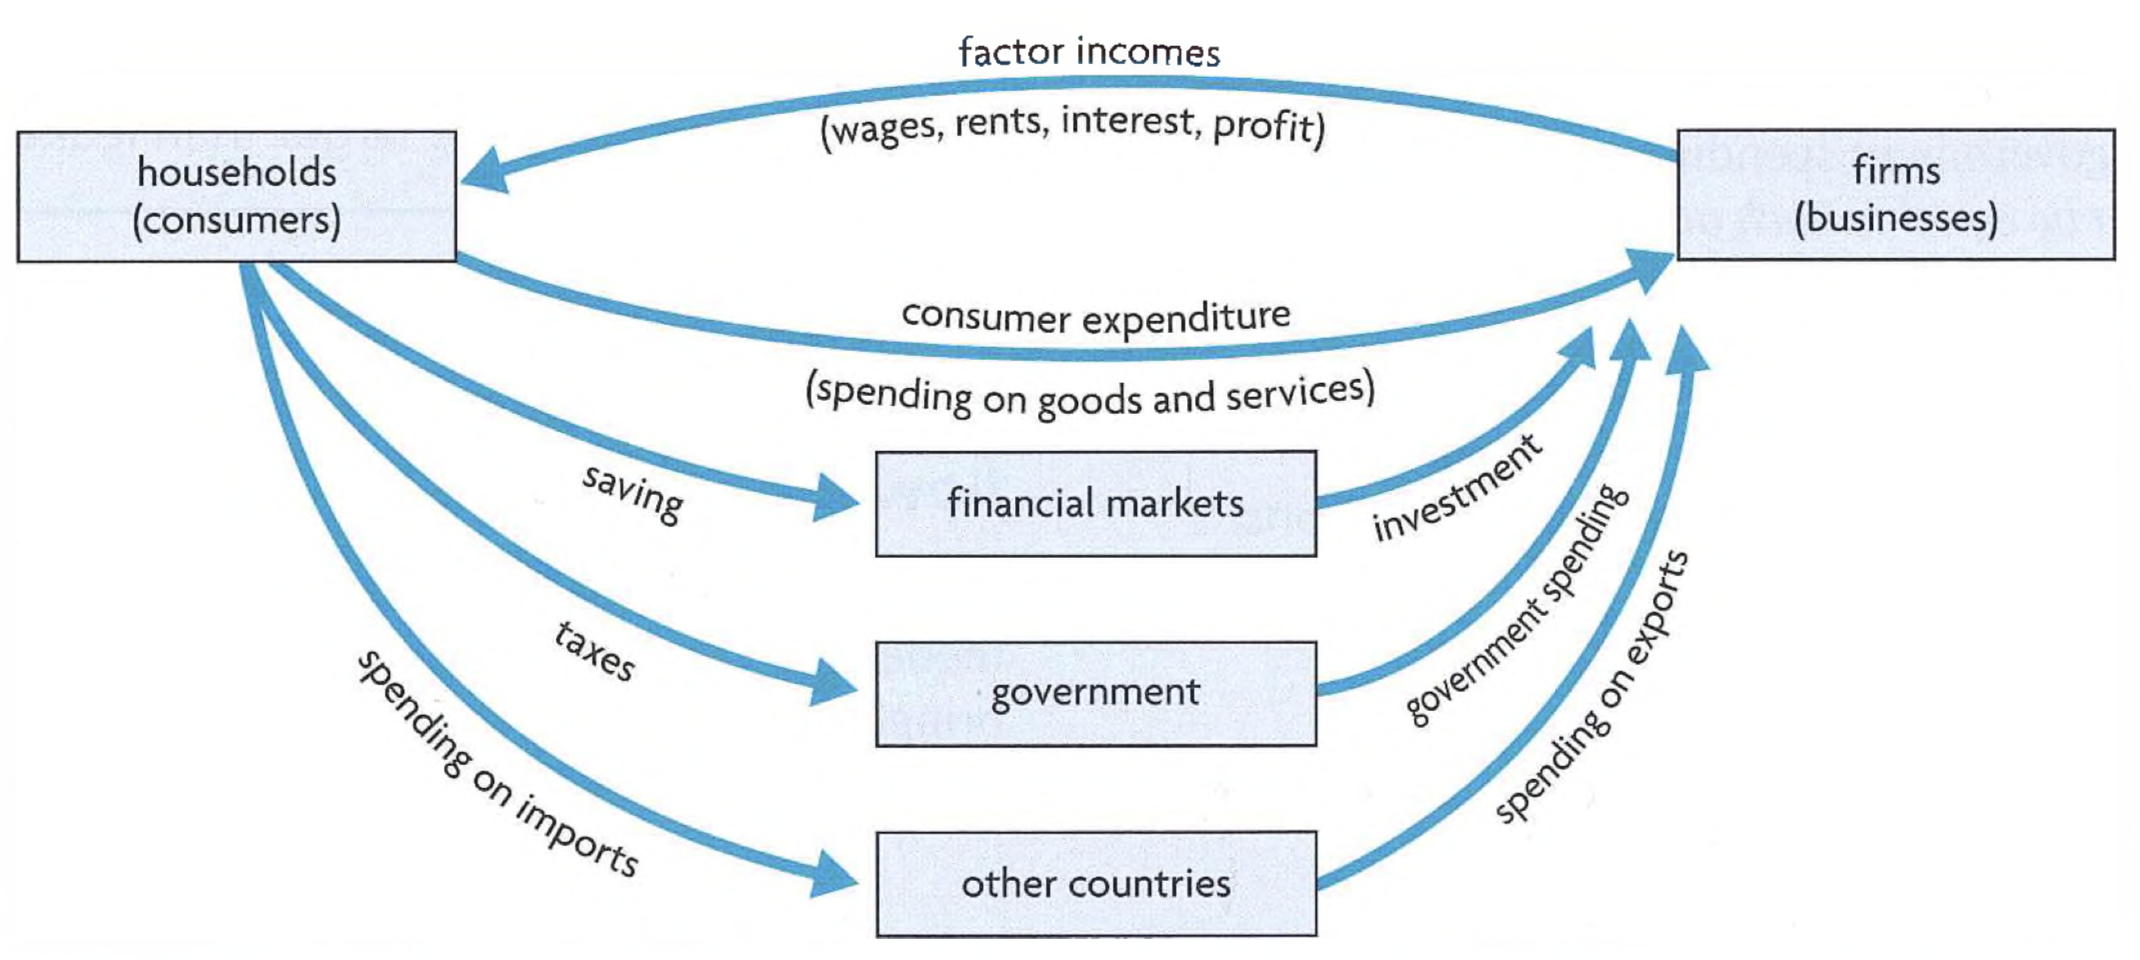
\includegraphics[width=0.6\linewidth]{Screenshot 2026-07-14 at 10.42.23.png}
\end{center}
The circular flow of income shows that in any given time period (say a year), the value of output produced in an economy is equal to the total income generated in producing that output, which is equal to the expenditures made to purchase that output.\\\\
Leakages from the circular flow of income (saving, taxes and imports) are matched by injections into the circular flow of income (investment, government spending and exports), though these need not be equal to each other. If injections are smaller than leakages, the income flow becomes smaller; if injections are larger
than leakages the income flow becomes larger.
\subsection{Measures of economic activity}
National income accounting: measuring an economy's national income or the value of output.\\
National output / aggregate output: total output of an economy.\\
There are three ways to measure the value of national output:
\begin{itemize}
  \item the expenditure approach adds up all spending to buy final (ready for final use) goods and services produced within a country over a time period
  \begin{itemize}
    \item Consumption, C, includes all purchases by households on final goods and services in a year.
    \item Investment spending, I, spending by firms on capital goods (i.e. buildings, machinery, equipment, etc.) and spending on new construction (housing and other buildings).
    \item Government expenditure, G, spending by governments within a country (national, regional, local).
    \item Net exports, (X-M), value of all exports (abbreviated as X) minus the value of all imports (abbreviated as M).
  \end{itemize}
  With all of these combined, you get $GDP=C+I+G+(X-M)$, the market value of all final goods and services produced in a country over a time period.
  \item the income approach adds up all income earned by the factors of production that produce all goods and services within a country over a time period (since the national income is equal to value of total output in the economy)
  \begin{itemize}
    \item Whereas national income is often used as a measure of the level of economic activity, it is not the same as GDP. 
    \item This approach allows economists to see the relative income shares of the different factors of production, how these might change over time, and to make comparisons over time or across countries.
  \end{itemize}
  \item the output approach calculates the value of all final goods and services produced in a country over a time period.
  \begin{itemize}
    \item The output approach calculates the value of output by economic sector.
    \item The value of output of each sector is then added up to obtain the total value of output for the entire economy.
    \item Sometimes the output of an economy is produced by factors of production that belong to foreigners.
  \end{itemize}
\end{itemize}
GNI, gross national income: the total income received by the residents of a country, equal to the value of all final goods and services produced by the factors of production supplied by the country's residents regardless where the factors are located.\\\\
The meaning of ``gross'' in GDP/GNI (supplementary): capital goods (buildings, machinery, equipment) wear out over time; the worn-out capital is called \needbold{depreciation} (also \textit{capital consumption}). In any year, total (gross) investment is split into:
\begin{itemize}
  \item the part that \textbf{replaces worn-out capital} (depreciation), and
  \item the part that is \textbf{new additions} of capital --- \needbold{net investment}.
\end{itemize}
\[\text{Gross investment} = \text{Depreciation} + \text{Net investment}\]
In $GDP = C + I + G + (X - M)$, the $I$ refers to \textbf{gross investment} (GDP measures total output, including replacement of worn-out capital). If instead we want net output, we use net investment $I_n$:
\[\text{NDP} = C + I_n + G + (X - M) = GDP - \text{depreciation}\]
Nominal values: money value, or value measured in terms of prices that prevail at the time of measurement. \\
Real value: a measure of value that takes into account changes in prices over time.\\\\
Total: measures of the value of output and income, provide a summary statement of the overall size of an economy.\\
Per capita: a summary measure of the standard of living in a country. (take population size into consideration)\\\\
PPP, purchasing power parities: the amount of a country's currency that is needed to buy the same quantity of local goods and services that can be bought with USD\$1 in the US (a measure of purchasing power)
\subsection{Calculations based on national income accounting}
Recall that $GDP=C+I+G+(X-M)$. \\
$GNI=GDP + \text{(income from abroad - income sent abroad)} / \text{net income from abroad}$.\\\\
Nominal GDP measures the value of current output valued at current prices, while real GDP measures the value of current output valued at constant (base year) prices.\\
A price index is a measure of average prices in one period relative to average prices in a base year.
\[\text{GDP Deflator}=\dfrac{\text{Nominal GDP}}{\text{Real GDP}}\times 100\]
Note that an increasing GDP deflator indicates rising prices on average, while a decreasing GDP deflator indicates falling prices on average.
\subsection{The business cycle}
Business cycles consist of short-term fluctuations in the growth of real output, which are alternating periods of expansion (increasing real output) and contraction (decreasing real output).
\begin{itemize}
  \item Expansion: occurs when there is positive growth in real GDP. During expansions, employment of resources increases, and the general price level of the economy usually begins to rise more rapidly.
  \item Peak: represents the cycle's maximum real GDP, and marks the end of the expansion. Unemployment of resources has fallen substantially, and the general price level maybe rising quite rapidly. Experiences inflation.
  \item Contraction: falling real GDP and growing unemployment of resources. (> 6 Months: recession)
  \item Trough: the cycle's minimum level of GDP, or the end of the contraction. Widespread unemployment.
\end{itemize}
While each cycle typically lasts several years, it is not possible to generalize, as there is wide variation in how long the cycle lasts, as well as in intensity.
\begin{center}
  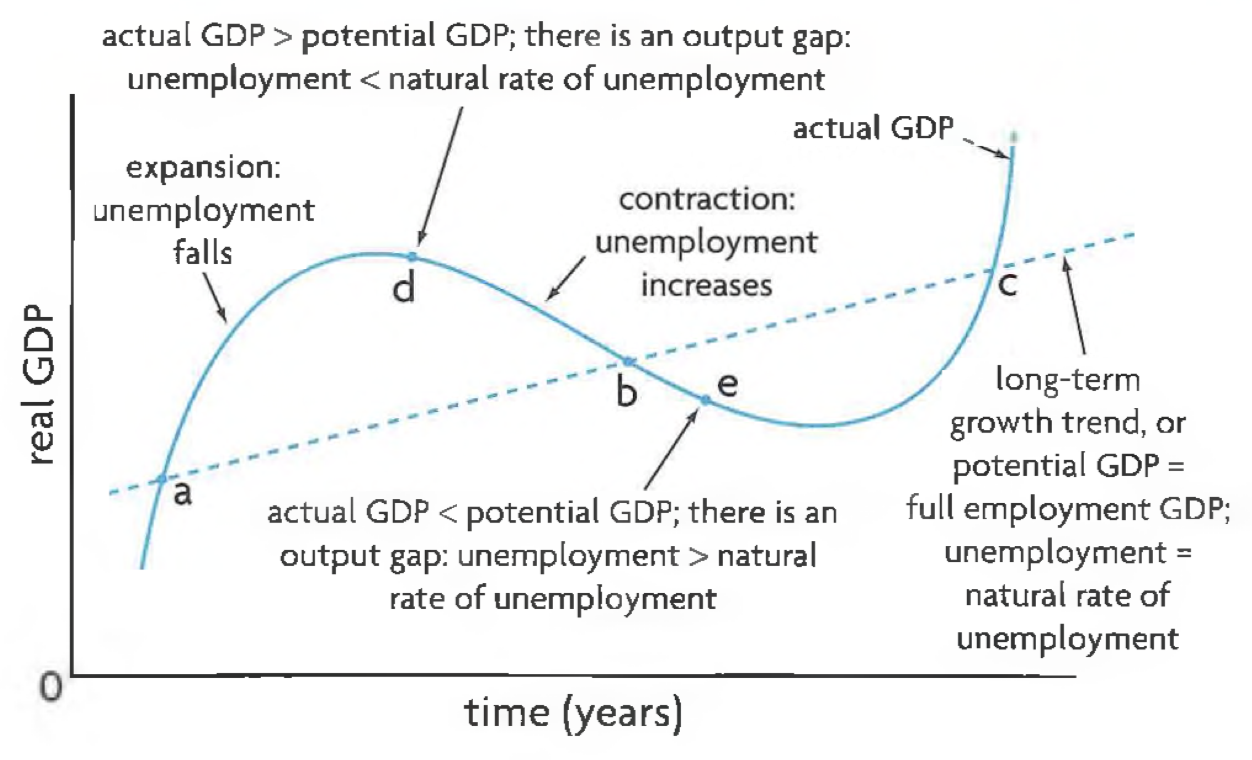
\includegraphics[width=0.6\linewidth]{Screenshot 2026-07-25 at 16.20.02.png}
\end{center}
The long-term growth trend shows how output grows over time when cyclical fluctuations are ironed out.\\\\
When real GDP fluctuates, it does so together with other macroeconomic variables, namely, unemployment of labor. Full employment is reached under the peak stage in the business cycle. \\
Whenever the economy produces its 'full employment level of output', there is still some unemployment, known as the 'natural rate of unemployment'. This is because at any time, there are some people who
are in between jobs, some who are moving from one geographical area to another, some people who are training or retraining to be able to get a new or better job, and some people who are temporarily out of work.\\\\
The output gap is simply actual GDP minus potential GDP, and may be positive or negative. \\\\
Using the business cycle, we can understand macroeconomic objectives to include:
\begin{itemize}
  \item Reducing the intensity of expansions and contractions: this is aimed at making output gaps as small as possible by flattening the cyclical curve.
  \item Increasing the steepness of the line representing potential output, meaning more rapid economic growth over long periods of time. 
\end{itemize}
\subsection{National income statistics and alternative measures}
\subsubsection*{Why GDP/GNI do not accurately measure the `true' value of output}
\begin{itemize}
  \item \textbf{Non-marketed output excluded}: goods/services not sold in markets (e.g.\ DIY home repairs, subsistence farming in developing countries) generate no income and are not recorded. Far larger in developing countries.
  \item \textbf{Underground (parallel) markets excluded}: legal transactions that go unreported (to avoid tax) plus illegal goods/services (drugs) are not recorded.
  \item \textbf{Quality improvements ignored}: technological advances improve products and lower prices, but GDP figures do not capture these consumer benefits.
  \item \textbf{Negative externalities not accounted for}: pollution, toxic waste and environmental degradation reduce well-being but are not deducted.
  \item \textbf{Depletion of natural resources ignored}: deforestation, loss of biodiversity and soil degradation lower future well-being but are not reflected.
  \item \textbf{Differing domestic price levels}: international comparisons are misleading unless adjusted using \textbf{purchasing power parities (PPP)} to account for differing price levels.
\end{itemize}
\subsubsection*{Why GDP/GNI cannot accurately measure economic well-being}
\begin{itemize}
  \item \textbf{No distinction in the composition of output}: military goods and merit goods (education, health care) both count equally in GDP; a country with lower GDP but more merit goods may have higher living standards.
  \item \textbf{Health, education and life expectancy unaccounted for}: two countries with equal GDP/GNI per capita may differ greatly in these dimensions.
  \item \textbf{No information on income distribution}: GDP per capita is an average --- it cannot reveal whether income is concentrated in a few hands or widely shared.
  \item \textbf{Leisure time excluded}: declining work hours increase well-being but do not appear in GDP.
  \item \textbf{Quality of life factors overlooked}: crime rates, security, political freedom, job security, stress, institutional quality.
\end{itemize}
\subsubsection*{Comparisons over time and between countries}
\begin{itemize}
  \item \textbf{Over time}: even using \textit{real} values, an increase in real GDP/GNI may over- or under-estimate true changes in well-being due to quality improvements, leisure, non-marketed output, underground markets, quality of life, etc.
  \item \textbf{Between countries}: one country may have higher GDP per capita but greater inequality, worse health/education, or more environmental damage than another with lower GDP.
\end{itemize}
\subsubsection*{Alternative measures of well-being}
图一乐 XD\\
\textbf{OECD Better Life Index}: developed by the OECD (36 member countries). Based on 11 indicators in two groups:
\begin{itemize}
  \item \textbf{Material conditions}: income \& wealth; jobs \& earnings; housing.
  \item \textbf{Quality of life}: health; work-life balance; education \& skills; social connections; \\civic engagement/governance; environmental quality; personal security; subjective well-being.
  \item Both depend on four types of \textbf{capital for future well-being}: natural, human, economic and social capital.
  \item \textit{Criticisms}: still under development; does not yet fully incorporate equity; some dimensions are hard to measure, limiting cross-country comparability.
\end{itemize}
\textbf{Happiness Index (World Happiness Report)}: compiled since 2012 by the UN Sustainable Development Network; covers 156+ countries. Based on:
\begin{itemize}
  \item real GDP per capita; social support; healthy life expectancy; freedom to make life choices; generosity; perceptions of corruption.
  \item Data from the \textbf{Gallup World Poll} (telephone surveys). Each country ranked 1--10 on each dimension plus an overall rank.
  \item \textit{Criticisms}: limitations of some data/variables; happiness is difficult to quantify and varies across cultures, weakening cross-country reliability.
\end{itemize}
\textbf{Happy Planet Index (HPI)}: developed by the New Economics Foundation (NEF), launched 2006 to challenge GDP growth as the primary policy goal. Measures \textbf{sustainable well-being}:
\[
\text{HPI} = \frac{\text{life expectancy} \times \text{well-being} \times \text{(inequality-adjusted)}}{\text{ecological footprint}}
\]
\begin{itemize}
  \item \textbf{Life expectancy}: average years a person expects to live (UN data).
  \item \textbf{Well-being}: population's life satisfaction (Gallup World Poll).
  \item \textbf{Inequality of outcomes}: decreases well-being and life expectancy.
  \item \textbf{Ecological footprint}: per-capita land needed for consumption + CO$_2$ absorption. Higher footprint $\to$ lower HPI.
  \item Covers 140--150 countries; scored 0--100.
  \item \textit{Focus}: sustainability, not personal happiness (unlike the Happiness Index).
  \item \textit{Criticisms}: well-being measure is controversial; the ecological footprint concept is debated.
\end{itemize}
\section{Aggregate demand and aggregate supply}
\subsection{Aggregate demand (AD) and the aggregate demand curve}
\needbold{Aggregate demand} is the total quantity of aggregate (total) output, or real GDP, that all buyers in an economy want to buy at different possible price levels, \emph{ceteris paribus}.
The aggregate demand (AD) curve shows the relationship between the total amount of real output demanded by the four components and the economy's price level over a particular time period. It is downward-sloping, indicating a negative relationship between the price level and aggregate output demanded.
\subsubsection*{Why the AD curve is downward-sloping (supplementary)}
In microeconomics, the downward slope of a demand curve is explained by diminishing marginal benefits; this reasoning \textbf{does not apply} to the aggregate demand curve. Instead, the negative slope is explained by three effects of a \textbf{change in the price level} (each is a \textit{movement along} AD):
\begin{itemize}
  \item \textbf{The wealth effect}: a higher price level reduces the \textit{real value of wealth} (savings, houses, stocks, bonds). People feel poorer and cut spending $\to$ less output demanded.
  \item \textbf{The interest rate effect}: a higher price level means consumers and firms need more money for transactions $\to$ demand for money rises $\to$ interest rates rise $\to$ borrowing is costlier $\to$ consumption and investment fall $\to$ less output demanded.
  \item \textbf{The international trade effect}: a higher domestic price level (with foreign price levels unchanged) makes exports more expensive and imports relatively cheaper $\to$ exports fall, imports rise $\to$ net exports $X - M$ fall $\to$ less output demanded.
\end{itemize}
\textbf{Clarification}: do not confuse these effects (price-level changes $\to$ \textbf{movements along} AD) with changes in wealth or interest rates that occur \textbf{without} a change in the price level (e.g.\ a stock-market boom, or the central bank changing interest rates) --- those cause \textbf{shifts} of the AD curve.
\subsubsection*{Determinants of AD curve shifts}
Meaning: for a certain price level, the amount of real GDP demanded increases / decreases.
\begin{itemize}
  \item \textbf{Consumption ($C$)} shifts:
  \begin{itemize}
    \item \textbf{Consumer confidence}: optimism $\to$ more spending $\to$ AD shifts right; pessimism (fear of unemployment/wage cuts) $\to$ AD shifts left.
    \item \textbf{Interest rates} (monetary policy): higher rates $\to$ borrowing more expensive $\to$ less spending $\to$ AD left; lower rates $\to$ AD right.
    \item \textbf{Wealth}: increase in asset values (houses, stocks) $\to$ feel wealthier $\to$ more spending $\to$ AD right; decrease $\to$ AD left.
    \item \textbf{Income taxes} (fiscal policy): higher taxes $\to$ lower disposable income $\to$ less spending $\to$ AD left; lower taxes $\to$ AD right.
    \item \textbf{Household indebtedness}: high debt $\to$ pressure to repay $\to$ cut spending $\to$ AD left; low debt $\to$ AD right.
    \item \textbf{Expected future prices}: expect prices to fall $\to$ postpone spending $\to$ AD left; expect prices to rise $\to$ buy now $\to$ AD right.
  \end{itemize}
  \item \textbf{Investment ($I$)} shifts:
  \begin{itemize}
    \item \textbf{Business confidence}: optimism about future sales $\to$ more investment $\to$ AD right; pessimism $\to$ AD left.
    \item \textbf{Interest rates} (monetary policy): higher rates $\to$ borrowing costlier $\to$ less investment $\to$ AD left; lower rates $\to$ AD right.
    \item \textbf{Technology improvements}: stimulate investment $\to$ AD right.
    \item \textbf{Business taxes} (fiscal policy): higher corporate taxes $\to$ lower after-tax profits $\to$ less investment $\to$ AD left; lower taxes $\to$ AD right.
    \item \textbf{Corporate indebtedness}: high debt $\to$ less willing to invest $\to$ AD left; low debt $\to$ AD right.
    \item \textbf{Legal/institutional changes}: improved access to credit, secured property rights $\to$ more investment $\to$ AD right (especially relevant in developing economies).
  \end{itemize}
  \item \textbf{Government spending ($G$)} shifts:
  \begin{itemize}
    \item \textbf{Political priorities}: changes in provision of merit/public goods, subsidies, pensions, salaries, etc.
    \item \textbf{Economic priorities}: deliberate use of government spending to influence AD (\textbf{fiscal policy}).
    \item Increase in $G$ $\to$ AD right; decrease in $G$ $\to$ AD left.
  \end{itemize}
  \item \textbf{Net exports ($X - M$)} shifts:
  \begin{itemize}
    \item \textbf{National income abroad}: higher foreign income $\to$ foreigners buy more exports $\to$ $X$ increases $\to$ AD right; lower foreign income $\to$ AD left.
    \item \textbf{Exchange rates}: domestic currency appreciates $\to$ exports more expensive (fall), imports cheaper (rise) $\to$ $X - M$ falls $\to$ AD left; currency depreciates $\to$ $X - M$ rises $\to$ AD right.
    \item \textbf{Trade protection}: foreign country imposes restrictions on imports $\to$ domestic exports fall $\to$ AD left; domestic country imposes restrictions $\to$ imports fall $\to$ $X - M$ rises $\to$ AD right.
  \end{itemize}
\end{itemize}
Note that income is not included among the factors that can shift the AD curve.
\subsection{SRAS and short-run equilibrium in the AD-AS model}
\needbold{Aggregate supply} is the total quantity of goods and services produced in an economy (real GDP) over a particular time period at different price levels.\\
The short-run aggregate supply curve (SRAS) shows the relationship between the price level and the quantity of real output (real GDP) produced by firms when resource prices (especially wages) do not change / in the short run. The SRAS curve is upward-sloping (linked with firm profitability), indicating that there is a positive (or direct) relationship between the price level and real GDP supplied.
\subsubsection*{Determinants of SRAS curve shifts}
Meaning: for any particular price level, firms produce a larger / smaller quantity of real GDP.
\begin{itemize}
  \item \textbf{Changes in wages}: higher wages (price level constant) $\to$ higher costs of production $\to$ SRAS shifts \textbf{left}; lower wages $\to$ SRAS shifts \textbf{right}.
  \item \textbf{Changes in non-labour resource prices}: increases in prices of oil, equipment, capital goods, land, etc.\ affect SRAS the same way as wages $\to$ higher prices shift SRAS \textbf{left}; lower prices shift SRAS \textbf{right}.
  \item \textbf{Changes in indirect taxes}: treated by firms as production costs $\to$ higher indirect taxes $\to$ SRAS \textbf{left}; lower taxes $\to$ SRAS \textbf{right}.
  \item \textbf{Changes in subsidies to businesses}: opposite effect of taxes $\to$ increased subsidies $\to$ SRAS \textbf{right}; decreased subsidies $\to$ SRAS \textbf{left}.
  \item \textbf{Supply shocks}: sudden, strong impacts on aggregate supply. Negative shocks $\to$ SRAS shifts \textbf{left}; positive shocks $\to$ SRAS shifts \textbf{right}.
\end{itemize}
In the AD-AS model, the equilibrium level of output occurs where aggregate demand intersects aggregate supply. Short-run equilibrium is given by the point of intersection of the AD and SRAS curves, and determines the price level, the level of real GDP and the level of employment.
\begin{center}
  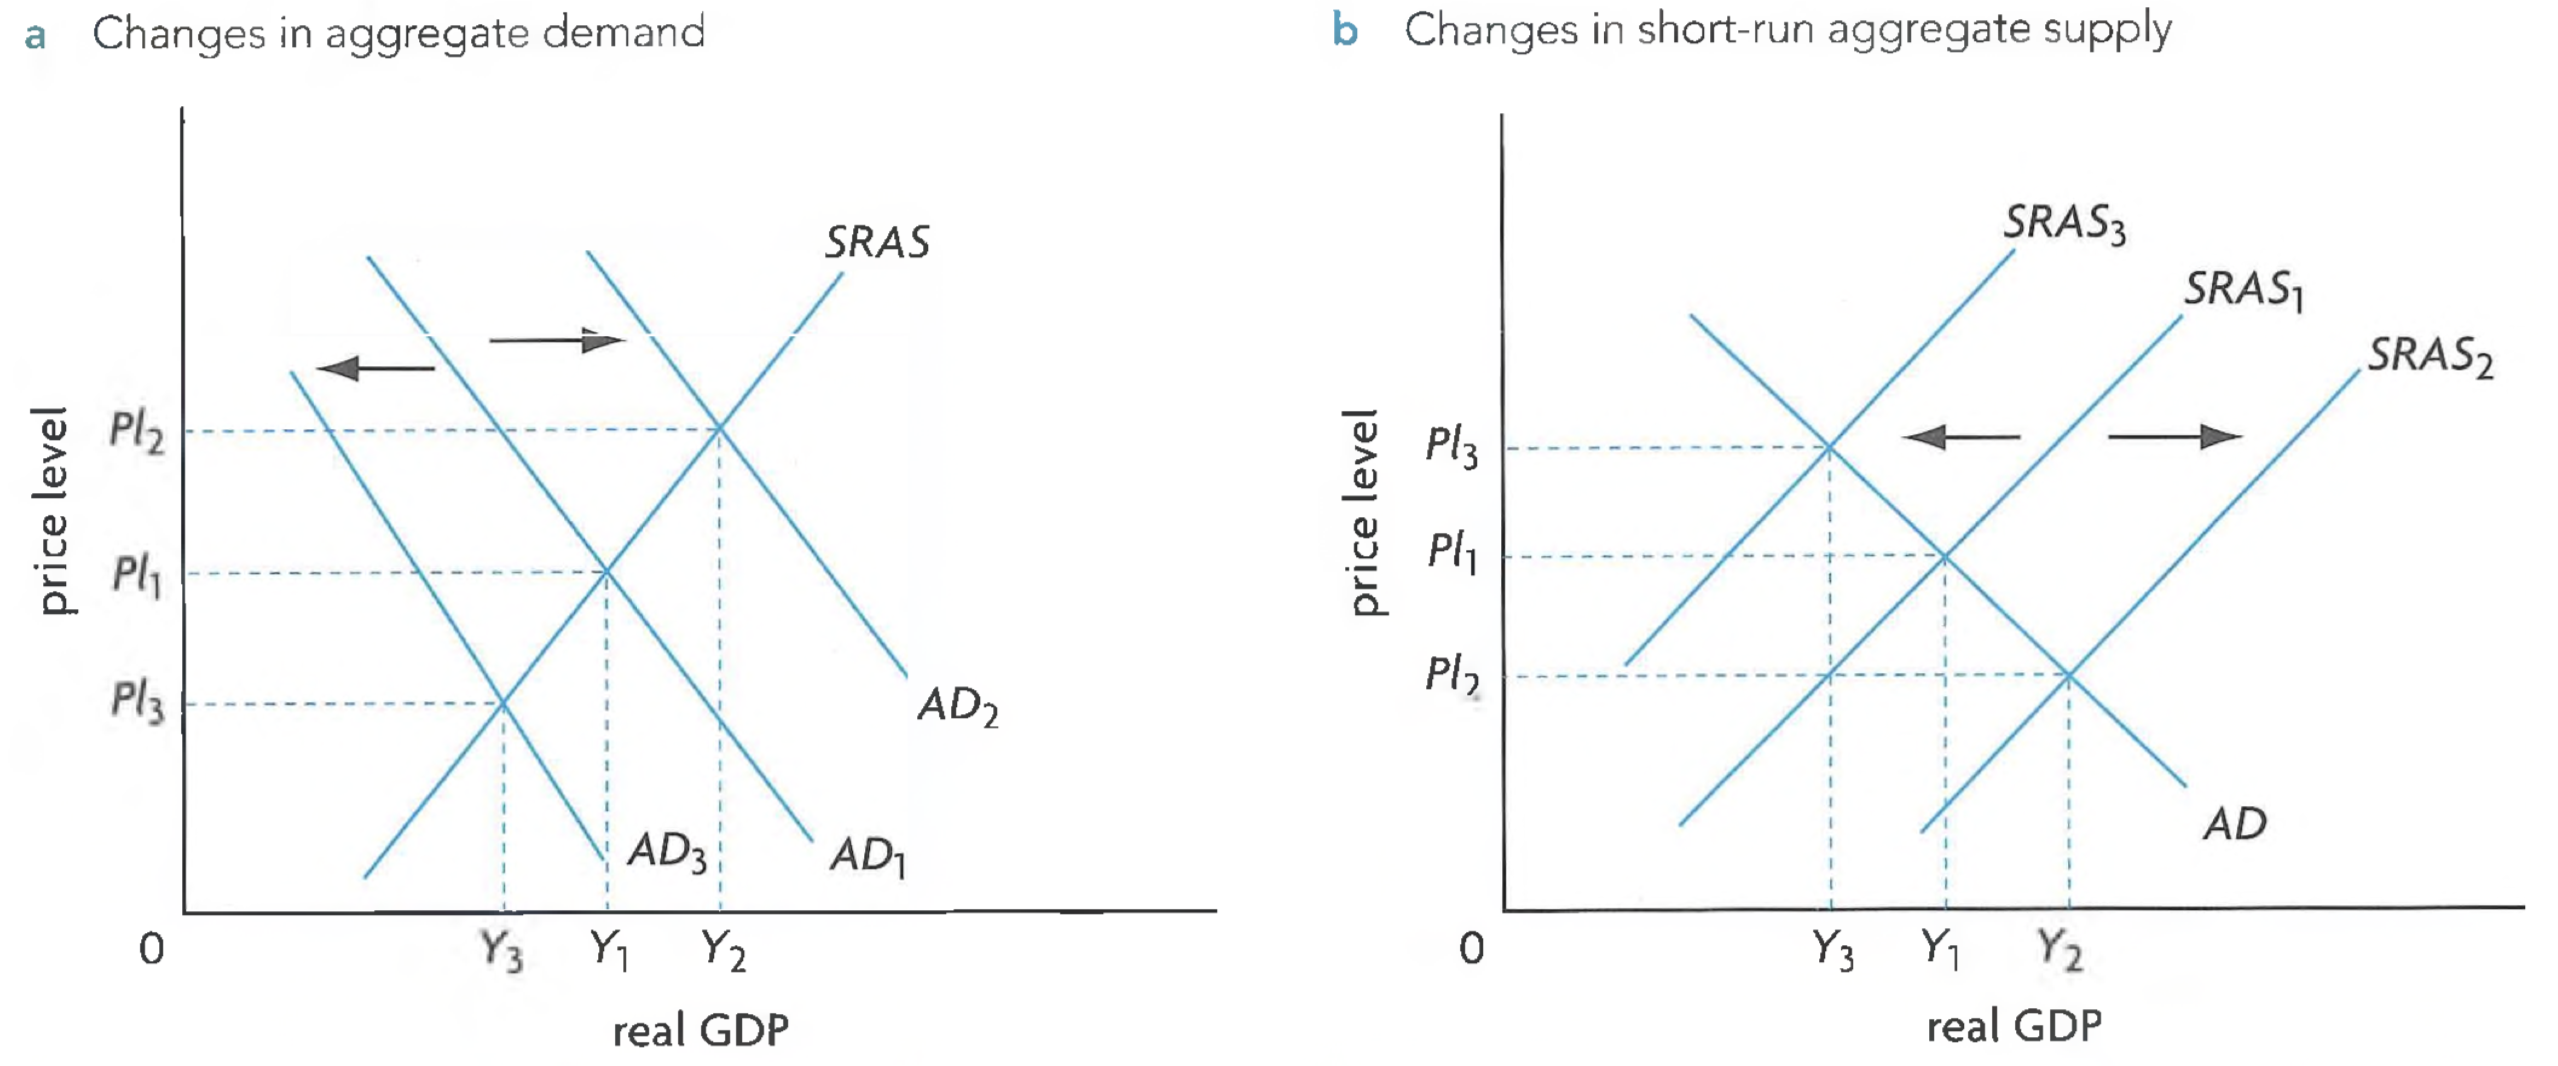
\includegraphics[width=0.99\linewidth]{Screenshot 2026-07-25 at 17.01.31.png}
\end{center}
Note that the level of employment is directly correlated with the real GDP.
\subsection{LRAS and long-run equilibrium in the monetarist/new classical model}
LRAS curve is vertical at potential GDP, also known as the full employment level of real GDP. A vertical LRAS curve means that in the long run any change in AD results only in changes in the price level while the quantity of real GDP produced remains the same. The economy is in long-run equilibrium
when the AD curve and the SRAS curve intersect at any point on the LRAS curve.
\begin{center}
  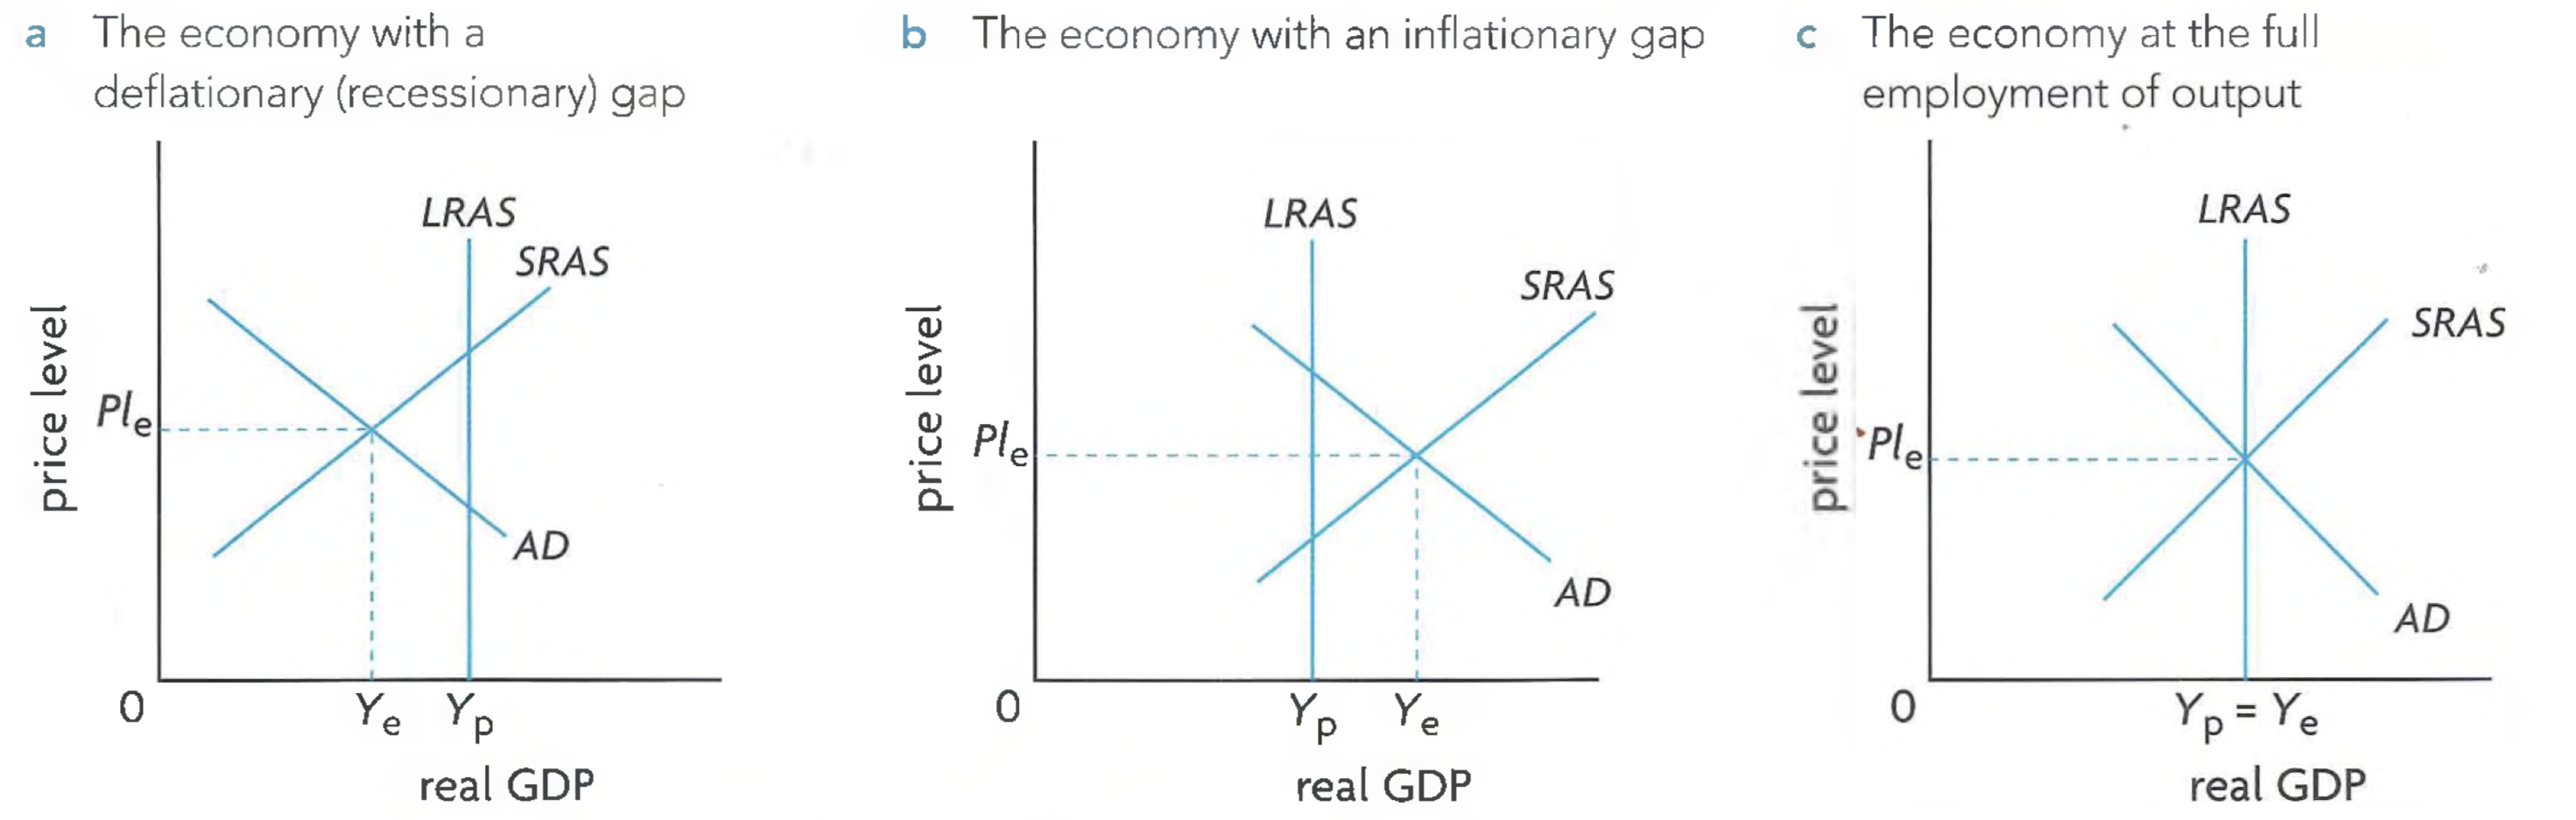
\includegraphics[width=0.9\linewidth]{Screenshot 2026-07-25 at 17.05.21.png}
\end{center}
The unemployment that exists when the economy is producing its full employment output is known as the natural rate of unemployment.
Explanation for the vertical shape of the LRAS curve: since wages (and other resource prices) are now changing to match output price changes, firms' costs of production remain constant even as the price level changes.
\subsubsection*{Short-run equilibrium positions in relation to long-run equilibrium}
\begin{itemize}
  \item deflationary gaps: real GDP is less than potential GDP, unemployment is greater than the natural rate of unemployment. There is not enough total demand in the economy to make it worthwhile for firms to produce potential GDP.
  \item inflationary gap: real GDP is larger than potential GDP, unemployment is less than the natural rate of unemployment. There is too much total demand in the economy, and firms respond by producing a greater quantity of real GDP than potential GDP.
  \item Full employment level of real GDP, or potential output: real GDP is equal to full employment or potential GDP. 
\end{itemize}
\subsubsection*{Causes of business cycle / short term fluctuations}
Shifts in AD (more frequent) and SRAS curves.
\begin{center}
  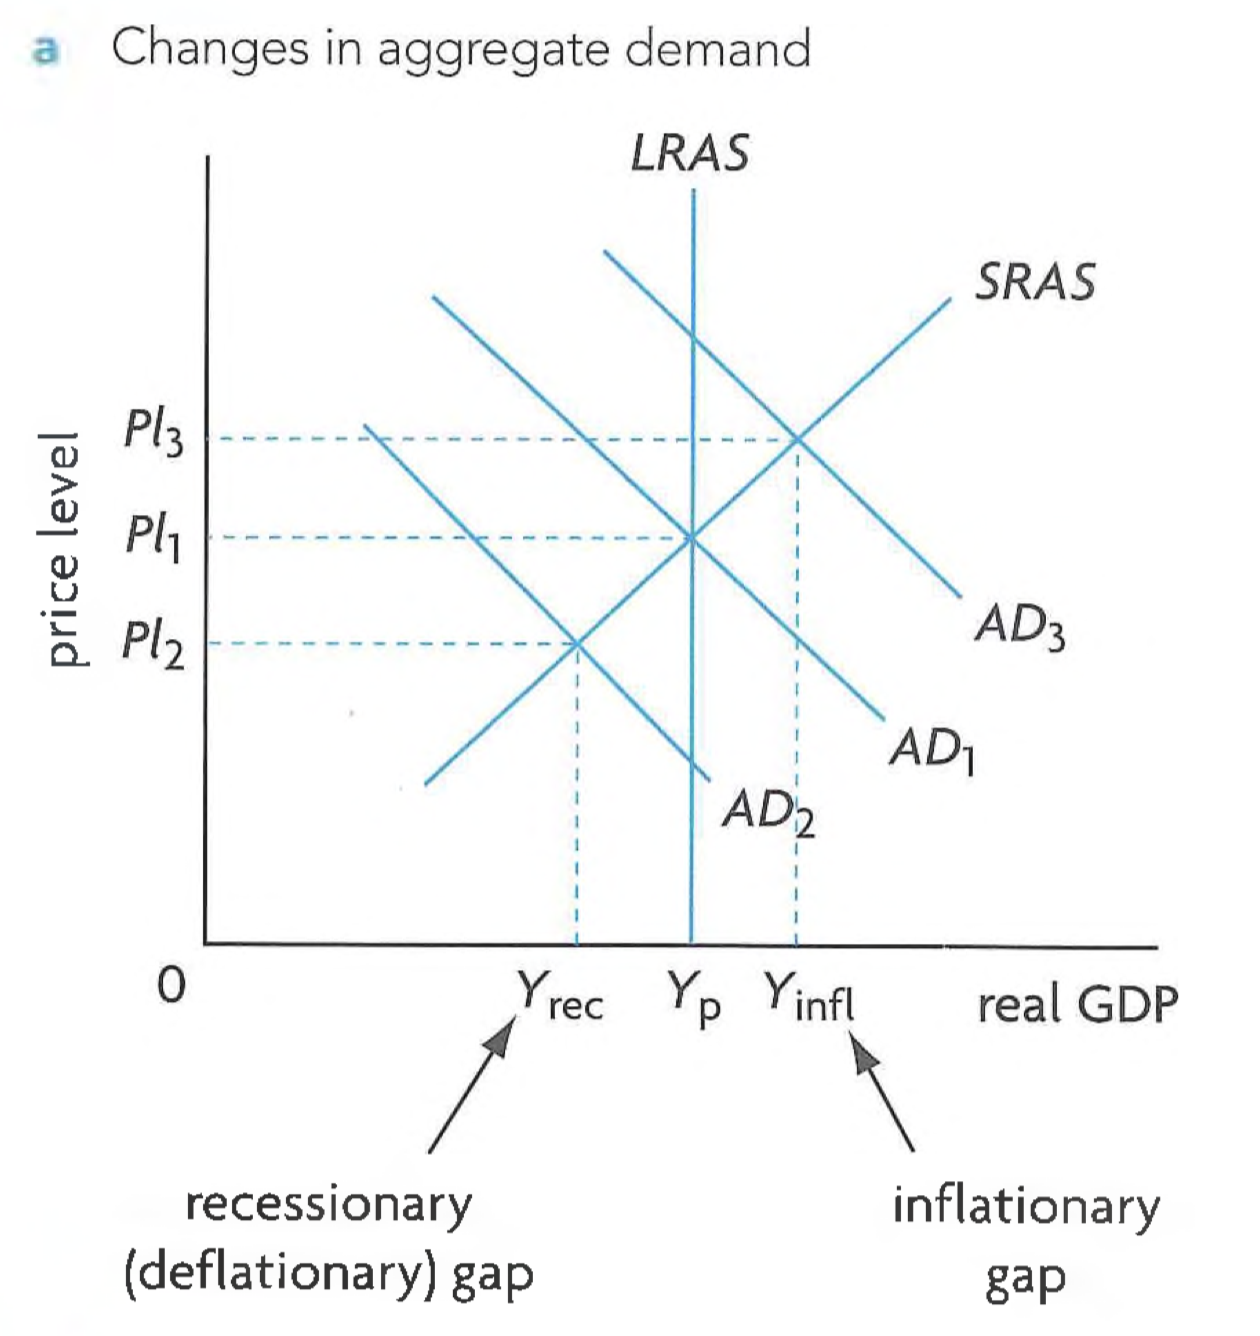
\includegraphics[width=0.4\linewidth]{Screenshot 2026-07-25 at 20.13.22.png}
  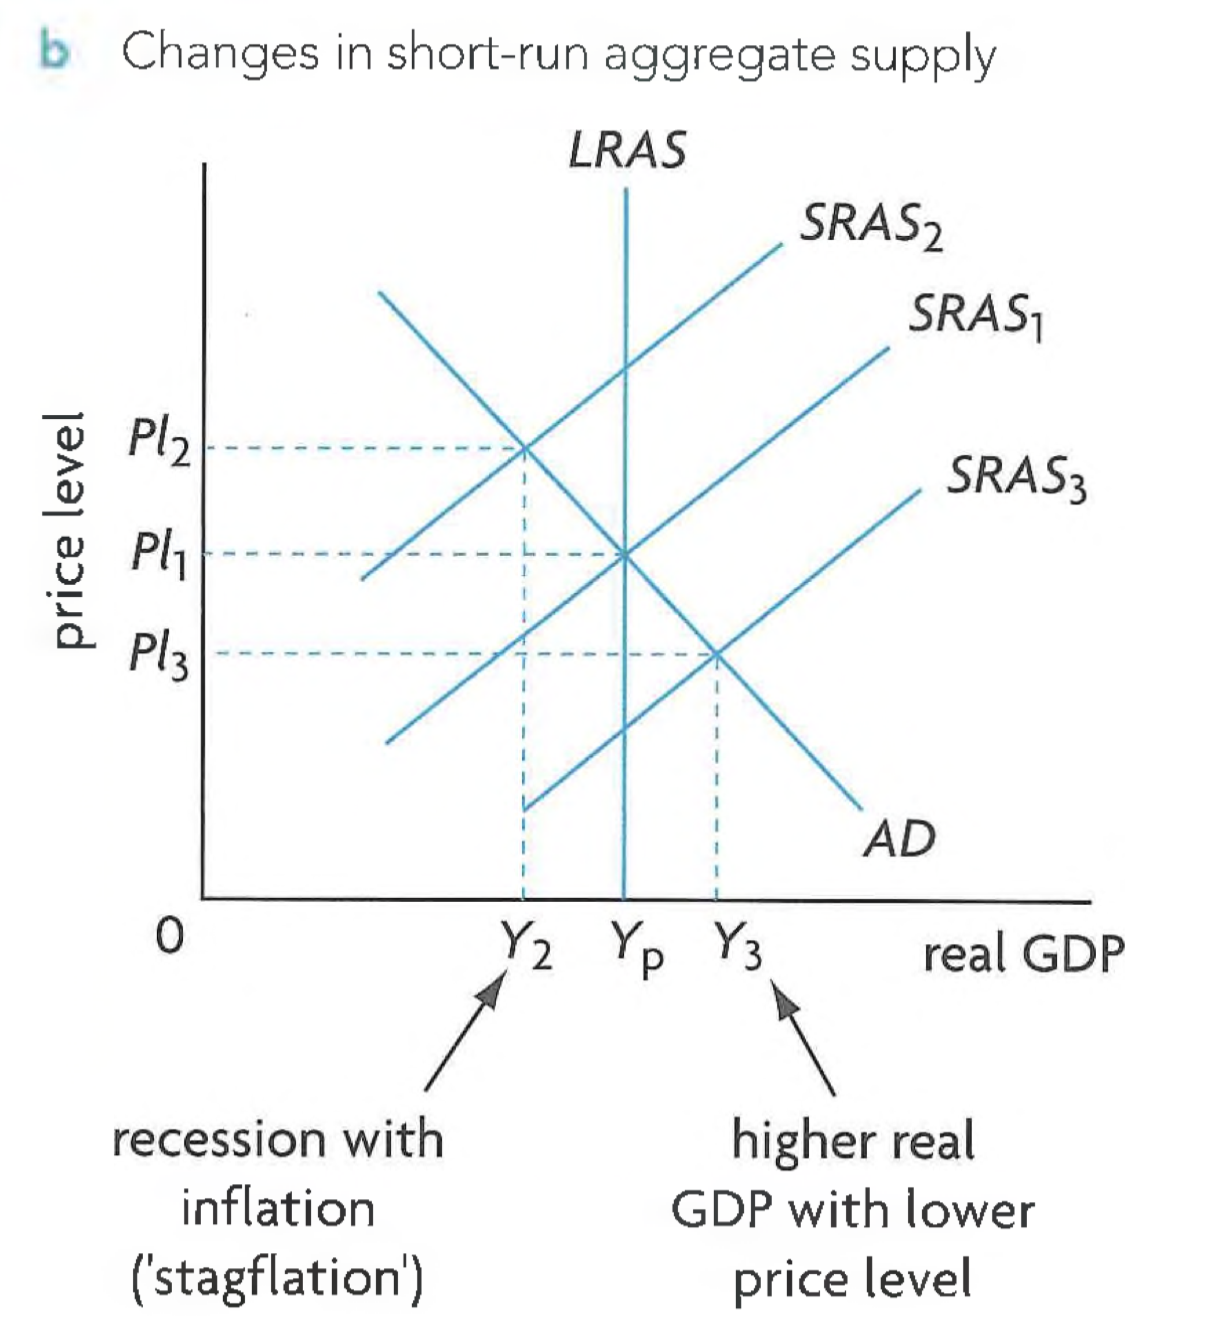
\includegraphics[width=0.38\linewidth]{Screenshot 2026-07-25 at 20.13.40.png}
\end{center}
In the long run, the gaps disappear, and the economy achieves full employment equilibrium. 
\\In the monetarist/new classical perspective, changes in aggregate demand can have an influence on real GDP only in the short run; in the long run, the only impact of a change in aggregate demand is to change the price level, having no impact on real GDP, as this remains constant at the level of potential or full employment output. Increase in AD in the long run only creates inflationary pressure.
\begin{center}
  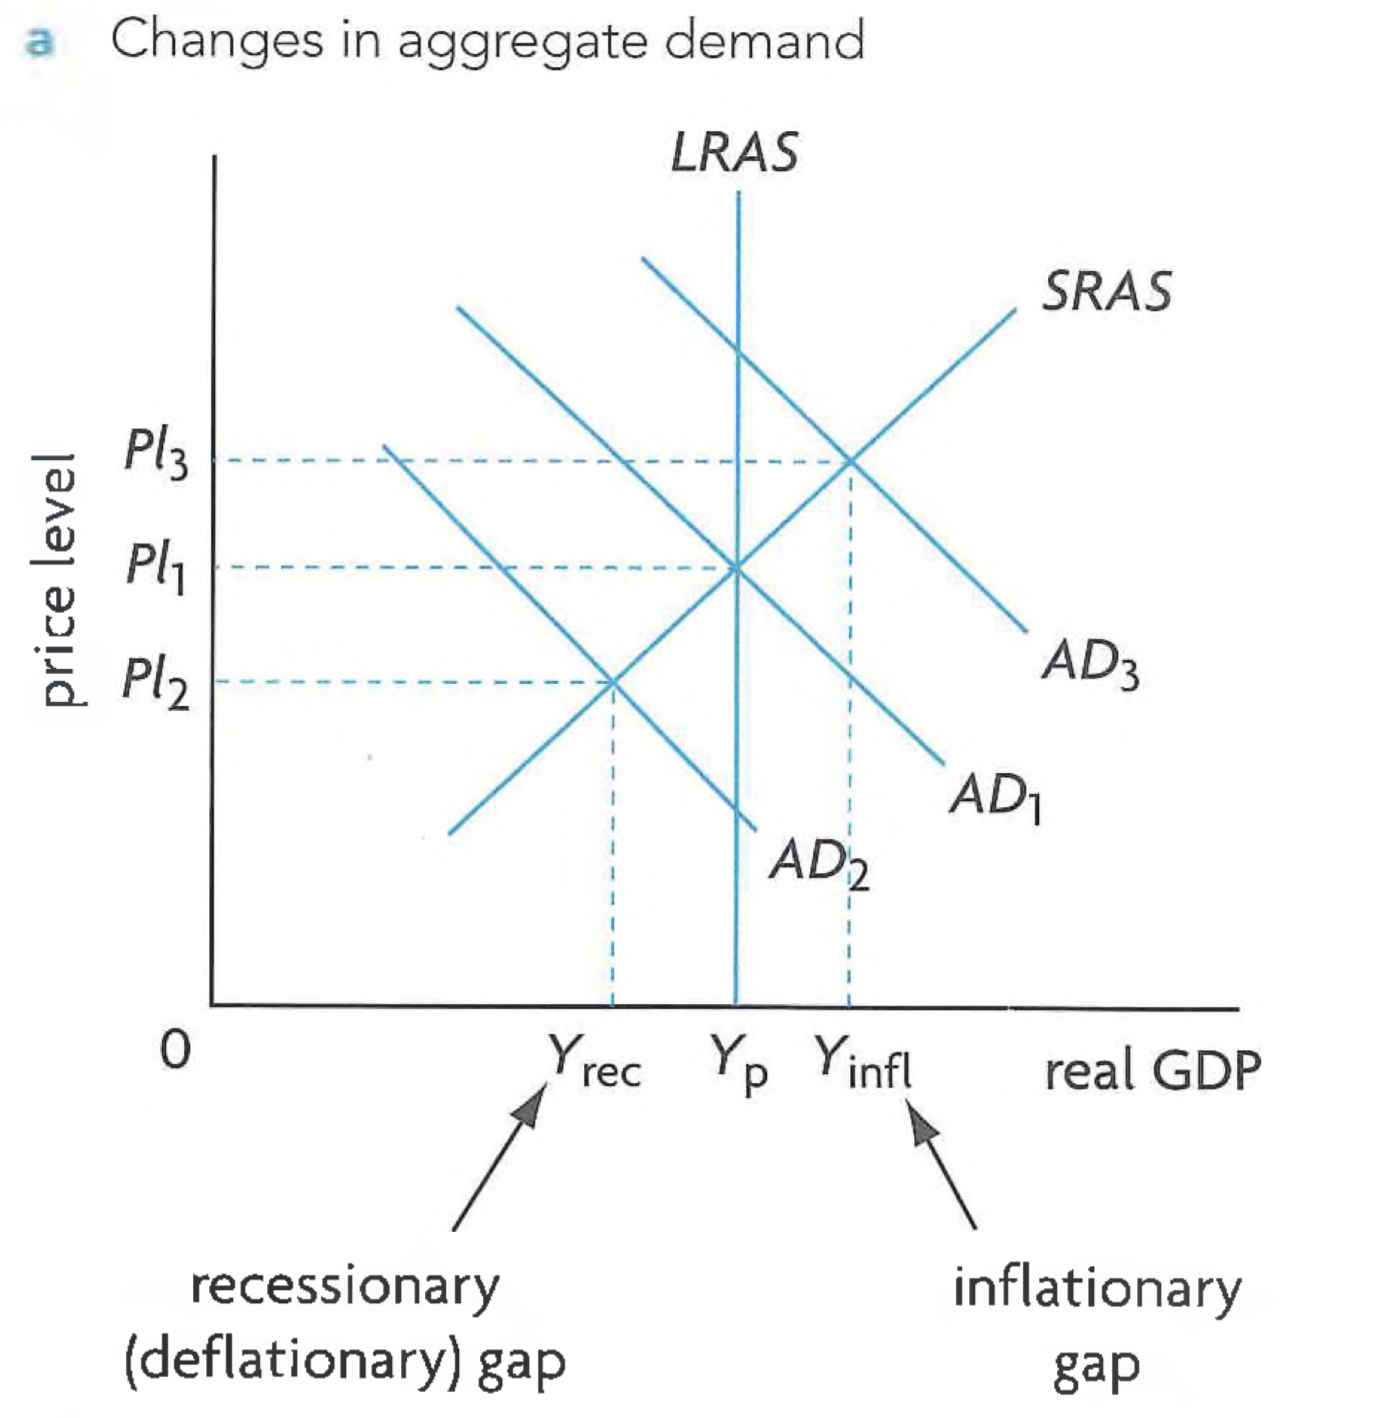
\includegraphics[width=0.32\linewidth]{Screenshot 2026-07-25 at 20.23.03.png}
  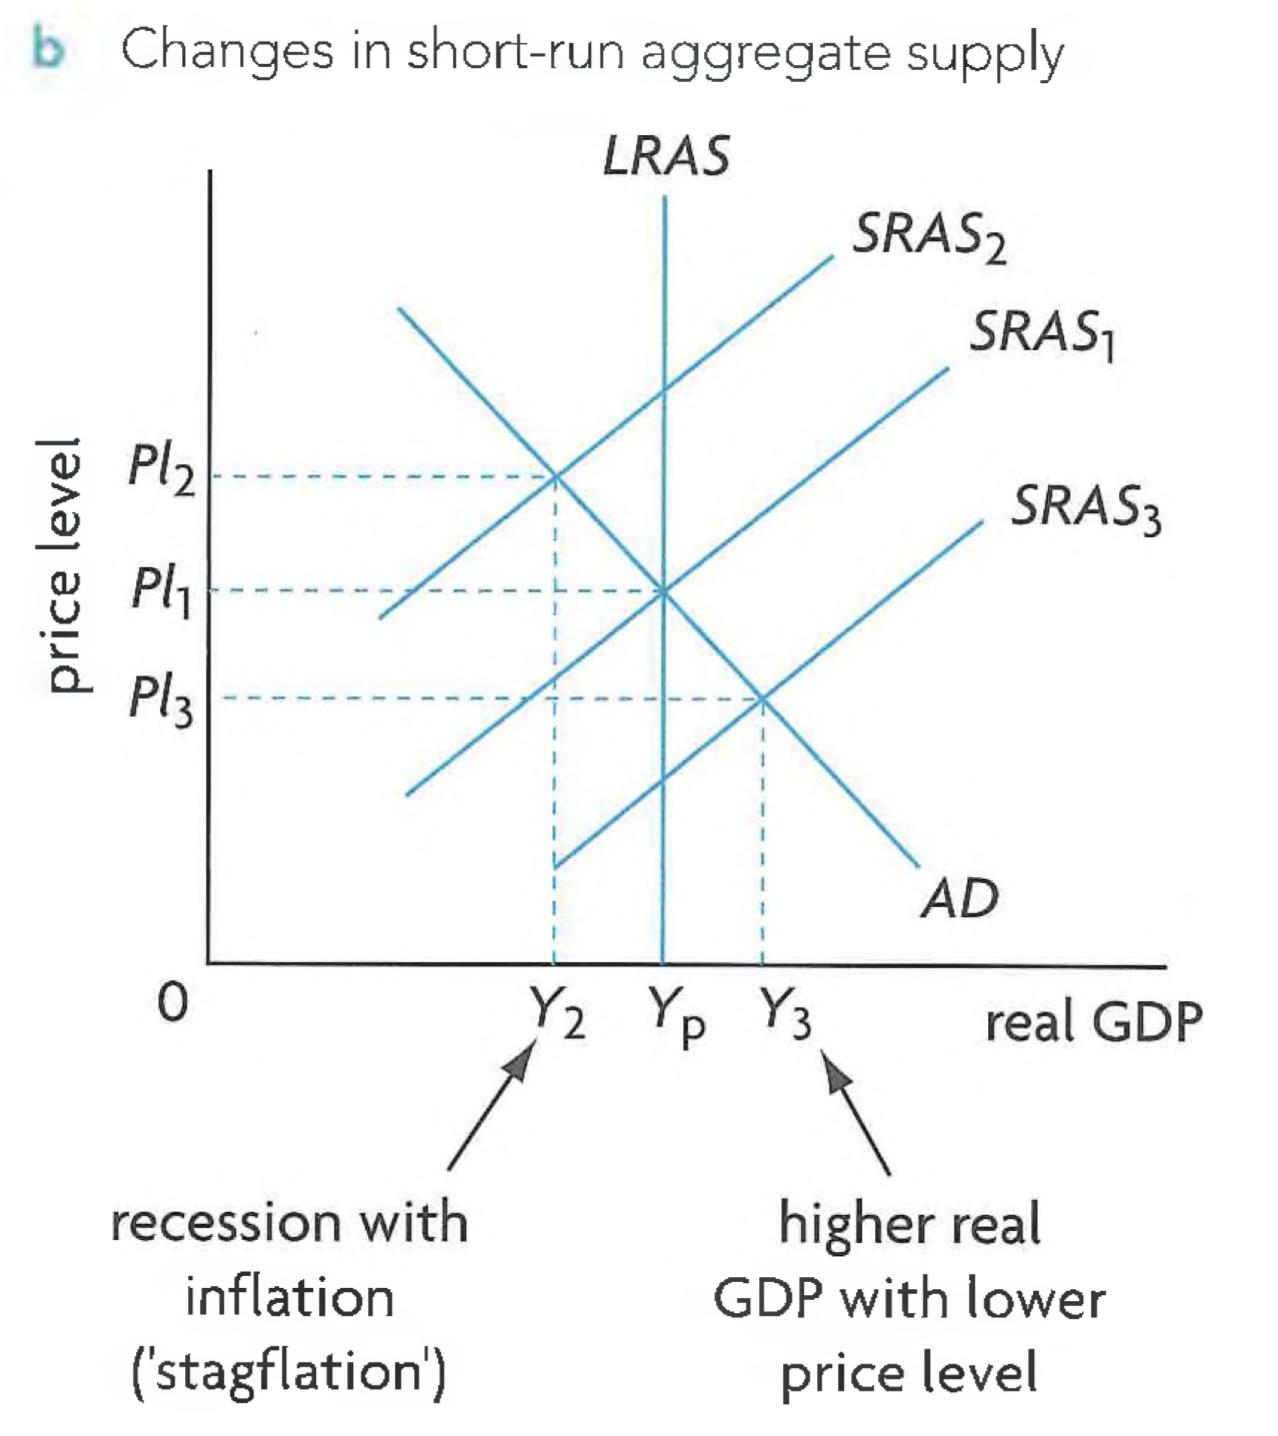
\includegraphics[width=0.3\linewidth]{Screenshot 2026-07-25 at 20.23.09.png}
\end{center}
\subsection{Aggregate supply and equilibrium in the Keynesian model}
\subsubsection*{Getting stuck in the short run}
Keynesian economists argue that there is an asymmetry between wage changes in the upward and downward directions.
\begin{itemize}
  \item Under conditions of an economic expansion and strong AD, with unemployment lower than the natural rate and a rising price level, wages quickly begin to move upward.
  \item in a recessionary gap, where AD is weak and the economy is in recession with unemployment greater than the natural rate, wages do not fall easily, even over long periods of time.
\end{itemize}
Keynesian economists also argue that not only wages but also product prices do not fall easily, even if an economy is in a recessionary gap. (To maintain profit and cover costs of production)\\\\
In the Keynesian model, inflexible wages and prices in the downward direction mean that the economy cannot move into the long run when experiencing a deflationary gap. Inflexible wages and prices are shown graphically by a horizontal section of the Keynesian aggregate supply (AS) curve.
\begin{center}
  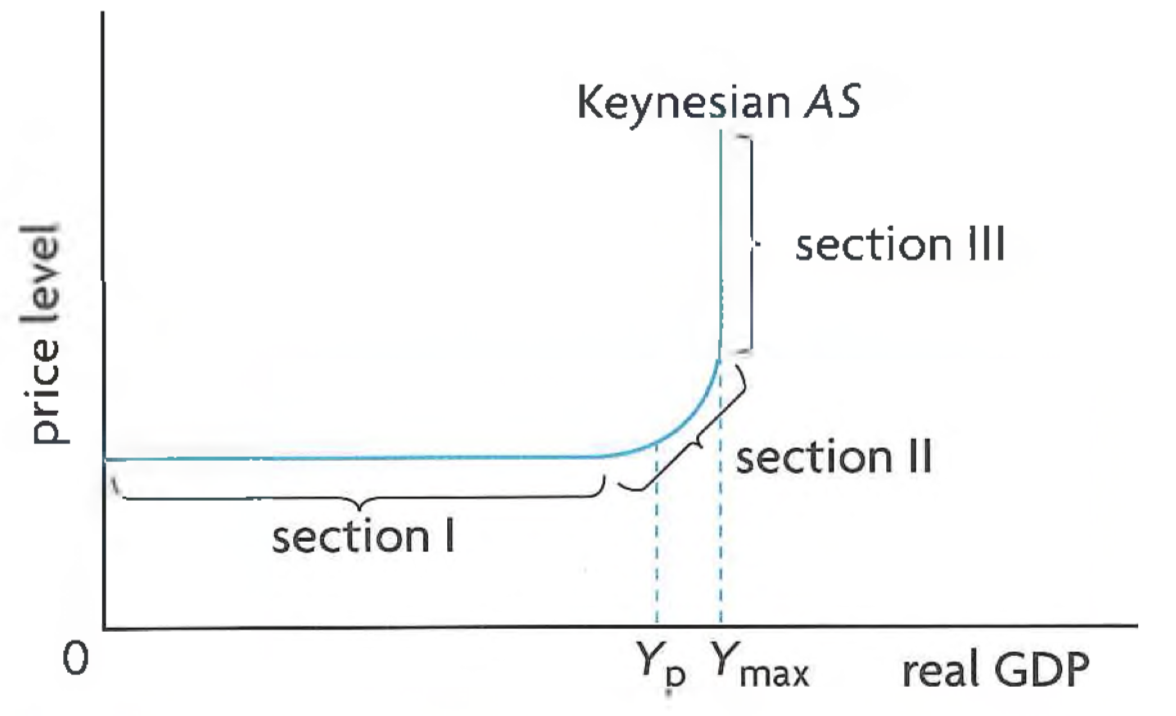
\includegraphics[width=0.5\linewidth]{Screenshot 2026-07-25 at 20.33.36.png}
\end{center}
\begin{enumerate}
  \item Real GDP is low, and the price level remains constant as real GDP increases. In this range of real GDP, there is a lot of unemployment of resources and spare capacity (free FoPs). When AD intersects in this region, the economy has a recessionary gap between $Y_e$ and $Y_p$.
  \item Real GDP increases are accompanied by increases in the price level. The reason is that as output increases, so does employment of resources, and eventually bottlenecks in resource supplies begin to appear as there is no longer spare capacity in the economy. CoP begins to increase. When AD intersects in this region, the economy reaches potential output for actual output.
  \item Real GDP reaches a level beyond which it cannot increase anymore; at this point, the price level rises very rapidly. Real GDP can no longer increase because firms are using the maximum amount of labour and all other resources in the economy. Any efforts on the part of firms to increase their output only result in greater increases in the price level. When AD intersects in this region, the economy experiences inflationary gap.
\end{enumerate}
\subsection{Shifting aggregate supply curves over the long term}
An increase in potential output signifies economic growth over the long term; a decrease signifies negative growth (or a fall in real output).
\subsubsection*{Determinants of long-term AS shifts}
\begin{itemize}
  \item \textbf{Increases in quantities of FoPs}: more physical capital, labour, land (e.g.\ discovery of new oil reserves) $\to$ economy can produce more real GDP. (Decreases shift left.)
  \item \textbf{Improvements in quality of FoPs}: better education, skills and health make workers more productive $\to$ more output per worker.
  \item \textbf{Improvements in technology}: improved machines/equipment from technological innovation $\to$ factors produce more output in the same time.
  \item \textbf{Increases in efficiency}: better use of scarce resources $\to$ greater potential output. (Decreases in efficiency shift left.)
  \item \textbf{Institutional changes}: degree of private vs.\ public ownership, competition, government regulation quality, bureaucracy --- all affect resource-use efficiency and output levels.
  \item \textbf{Reductions in the natural rate of unemployment}: fewer people unemployed $\to$ better resource utilisation $\to$ higher potential output. (Increases shift left.)
\end{itemize}
\subsubsection*{Monetarists / New Classical}
If an economy is experiencing long-term economic growth, its LRAS curve will be shifting rightward, indicating increases in potential output. Yet over long periods of
time, its SRAS curve will be shifting rightward as well. Any factor that shifts the LRAS curve must, over the long term, also shift the SRAS curve.\\\\
There are temporal changes to SRAS that wouldn't affect LRAS at all, such as temporal weather change, change in CoP etc. As an economy grows over time, it is likely that aggregate demand also increases. The reason is that many of the factors that cause the LRAS (and SRAS) curves to shift also cause the AD curve to shift.
\subsection{Implications of the Keynesian model and the monetarist/new classical model}
\subsubsection*{Automatic self-correction vs.\ persistence of deflationary gaps}
\begin{itemize}
  \item \textbf{Monetarist/new classical model}: inflationary and deflationary gaps are \textbf{automatically corrected} as long as wages and prices are free to change. The economy returns to full-employment equilibrium on its own.
  \item \textbf{Keynesian model}: deflationary/recessionary gaps can \textbf{persist indefinitely} due to (i) the inability of wages and prices to fall (sticky wages/prices) and (ii) \textbf{insufficient aggregate demand} --- the four components of AD cannot buy enough output to justify producing potential GDP, so equilibrium GDP $Y_e <$ potential GDP.
  \item Keynesian analysis is essentially \textbf{short-term}: Keynesians do not accept the monetarist idea that the economy automatically moves to a long-run full-employment equilibrium with flexible prices.
\end{itemize}
\textbf{Policy implications}:
\begin{itemize}
  \item Monetarist/new classical: governments should make markets work freely (flexible wages/prices) with \textbf{minimal interference}; focus on \textbf{shifting LRAS right} (supply-side policies).
  \item Keynesian: the government \textbf{must intervene} to increase AD and close the deflationary gap.
\end{itemize}
\subsubsection*{Increases in AD and the price level}
\begin{itemize}
  \item \textbf{Monetarist/new classical}: increases in AD \textbf{always cause price-level increases} --- in the short run (movement along upward-sloping SRAS, both real GDP and PL rise) and in the long run (only PL rises; real GDP unchanged). $\therefore$ policy should focus on \textbf{long-run growth} (shifting LRAS right).
  \item \textbf{Keynesian}: when the economy is on the \textbf{horizontal} part of the AS curve (deflationary gap), increases in AD raise \textbf{real GDP only}, with \textbf{no change in the price level}. Price-level increases begin only as the AS curve slopes upward near full employment; when the AS curve is vertical, AD increases cause only inflation. $\therefore$ policies to increase AD are \textbf{harmless and essential} when the economy is in a deflationary gap.
\end{itemize}
\section{Macroeconomic objectives I}
\subsection{Low unemployment}
\needbold{Unemployment}, in a general sense, refers to idle, or not fully used resources (referring to labors the most). \\
Unemployment refers to people of working age who are actively looking for a job but who are not employed.\\
\needbold{Underemployment}: people of working age with part-time jobs when they would rather work full time, or with jobs that do not make full use of their skills and education. \\
Both unemployment and underemployment mean that an economy is wasting scarce resources by not using them fully.\\\\
The \needbold{labor force}: the number of people who are employed (working) plus the number of people of working age who are unemployed (not working but seeking work).
\[\text{Unemployment rate}=\dfrac{\text{Unemployed}}{\text{Labor force}}\times 100\]
Difficulties in measuring unemployment: (underestimation: hidden unemployment; overestimation)
\begin{itemize}
  \item Unemployment figures include only unemployed persons who are \textbf{actively looking for work}. This excludes \textbf{marginally attached workers} --- people who want a job and have looked for one in the past 12 months but are \textit{not currently} searching (past 4 weeks) --- including \textbf{discouraged workers}, who gave up looking because they believe no jobs are available for them (see supplementary subsection below).
  \item Unemployment figures do not make a distinction between full-time and part-time employment, and count people with part-time jobs as having full-time jobs though in fact they are underemployed.
  \item Unemployment figures make no distinction on the type of work done. (Not regarding underemployment)
  \item Unemployment figures do not include people on retraining programmes who previously lost their jobs / people that have retired early.
  \item Unemployment figures do not include people working in the underground economy.
  \item National unemployment rate does not account for differences in unemployment that often arise among different population groups in a society. (factors including region, gender, ethnic groups, age, occupation and educational attainment)
\end{itemize}
\subsubsection*{Supplementary: Marginally attached workers and broader unemployment measures (AP)}
\needbold{Marginally attached workers} are people who \textbf{want a job}, have \textbf{looked for work sometime in the past 12 months}, but are \textbf{not currently counted as unemployed} because they have \textbf{not actively searched during the past 4 weeks}. Because they are not actively searching, they are classified as \textbf{out of the labour force} and are excluded from the official unemployment rate.
\begin{itemize}
  \item \needbold{Discouraged workers} are the primary subset of marginally attached workers: unemployed workers who \textbf{gave up looking for a job} because they believe no suitable jobs are available for them (due to lack of skills, age discrimination, or local economically depressed conditions). They represent the \textbf{hidden unemployed}.
  \item Other marginally attached workers stopped searching due to personal or family responsibilities, illness, or school attendance.
  \item \textbf{Significance for policy}:
  \begin{itemize}
    \item During economic downturns, many unemployed workers become discouraged and drop out of the labour force, causing the \textbf{official unemployment rate to understate the true severity of joblessness}.
    \item During recoveries, marginally attached workers re-enter the labour force and resume searching, causing the official unemployment rate to fall slowly or even temporarily rise.
    \item The \textbf{labour force participation rate} ($\text{Labour force} / \text{Working-age population}$) serves as an essential complement to the unemployment rate.
  \end{itemize}
  \item \textbf{Alternative (broader) unemployment measures} (US BLS / AP Macro):
  \begin{itemize}
    \item \textbf{U-3}: the official unemployment rate ($\text{Unemployed} / \text{Labour force}$).
    \item \textbf{U-4}: U-3 $+$ discouraged workers.
    \item \textbf{U-5}: U-4 $+$ all other marginally attached workers.
    \item \textbf{U-6}: U-5 $+$ involuntary part-time workers (underemployed workers seeking full-time jobs) --- the broadest measure of labour underutilisation.
  \end{itemize}
\end{itemize}
Costs of unemployment:
\begin{itemize}
  \item Economic costs
  \begin{itemize}
    \item A loss of real output (real GDP)
    \item A loss of income for unemployed workers
    \item A loss of tax revenue for the government. 
    \item Costs to the government of unemployment benefits.
    \item Costs to the government of dealing with social problems resulting from unemployment
    \item Larger budget deficit or smaller budget surplus.
    \item More unequal distribution of income. (unemployed becomes poorer)
    \item Unemployed people may have difficulties finding work in the future. (Loss of skills over time, know as \textit{hysteresis})
  \end{itemize}
  \item Personal and social costs
  \begin{itemize}
    \item Loss of income
    \item Increased indebtedness 
    \item Loss of self-esteem
    \item Increased rate of crime / violence
    \item Growing poverty
    \item ......
  \end{itemize}
\end{itemize}
Types and causes of unemployment:
\begin{itemize}
  \item \textbf{Structural unemployment}: caused by changes in demand for particular labour skills, changes in the geographical location of industries/jobs, and labour market rigidities.
  \begin{itemize}
    \item \textbf{Changes in labour skill demand}: technological change makes some skills obsolete while creating demand for new skills; structural shifts in the economy leave workers without the skills needed in growing industries $\to$ \textbf{mismatch} between skills demanded and supplied.
    \item \textbf{Geographical relocation of jobs}: when firms/industries move or close down, demand for labour falls in one region and rises in another; if workers cannot move to expanding regions, they become structurally unemployed.
    \item \textbf{Labour market rigidities}: factors preventing supply and demand from operating freely:
    \begin{itemize}
      \item \textbf{Minimum wage legislation}: wage set above equilibrium $\to$ excess supply of labour ($Q_s - Q_d$).
      \item \textbf{Labour union activities}: wage bargaining pushes wages above equilibrium.
      \item \textbf{Employment protection laws}: make firing costly $\to$ firms more cautious about hiring.
      \item \textbf{Generous unemployment benefits}: reduce incentive to work.
    \end{itemize}
    \begin{center}
      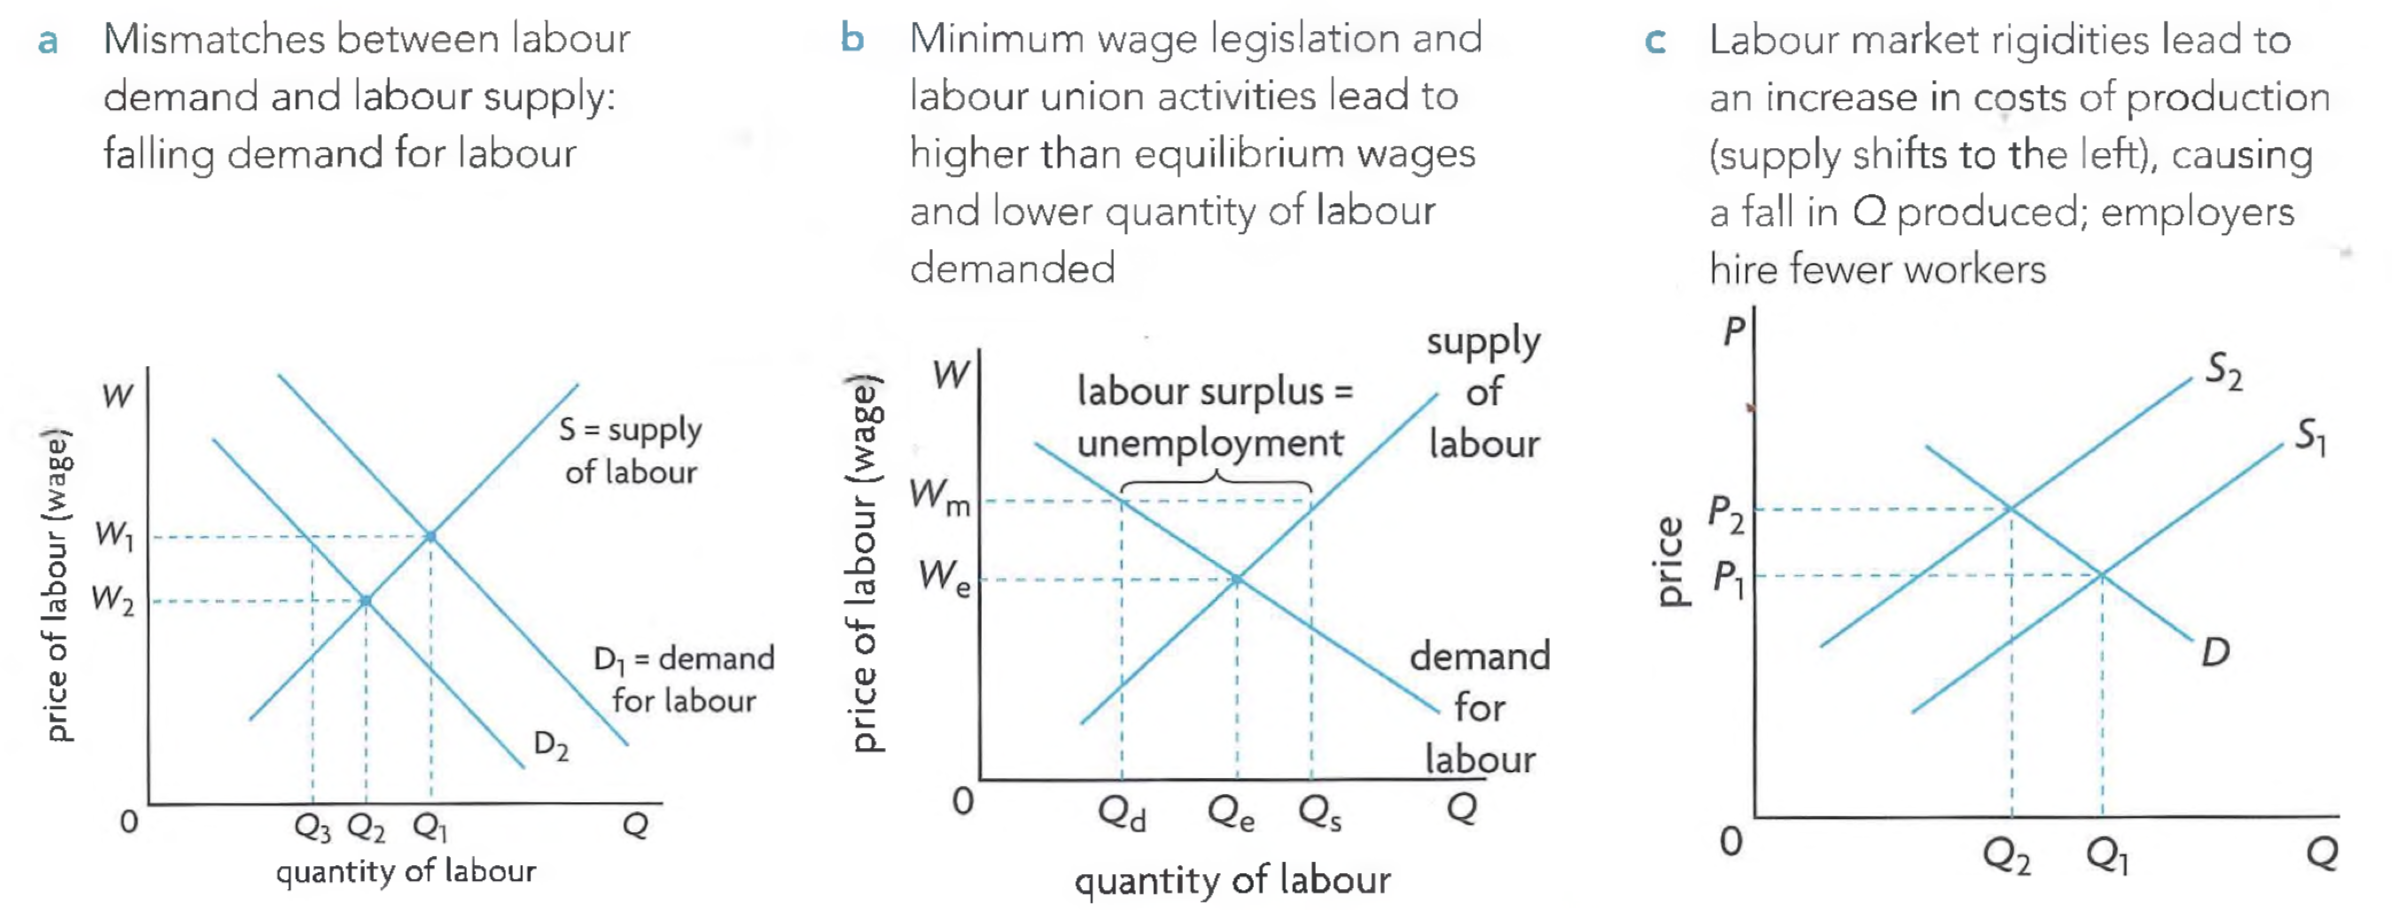
\includegraphics[width=0.9\linewidth]{Screenshot 2026-07-26 at 15.02.55.png}
    \end{center}
    \item Structural unemployment tends to be \textbf{long-term} and is part of \textbf{natural unemployment}, but can be reduced through retraining, relocation incentives, hiring subsidies, and reducing labour market rigidities.
  \end{itemize}
  \item \textbf{Frictional unemployment}: occurs when workers are \textbf{between jobs} (fired, searching for better jobs, waiting to start). Short-term; does not involve lack of in-demand skills. Caused partly by \textbf{incomplete information} between employers and workers about vacancies/qualifications. Part of \textbf{natural unemployment}; reducible by improving information flows and reducing search time.
  \item \textbf{Seasonal unemployment}: occurs when demand for labour varies \textbf{seasonally}. Some is unavoidable; part of \textbf{natural unemployment}.
  \item \textbf{Cyclical / demand-deficient unemployment}: occurs during \textbf{downturns of the business cycle} when the economy is in a deflationary/recessionary gap. Caused by \textbf{declining aggregate demand}: as real GDP falls, firms lay off workers. When AD recovers and real GDP returns to potential output, cyclical unemployment falls to \textbf{zero}. Illustrable in both monetarist/new classical and Keynesian AD-AS models (fall in AD $\to$ recessionary gap $\to$ cyclical unemployment).
  \begin{center}
    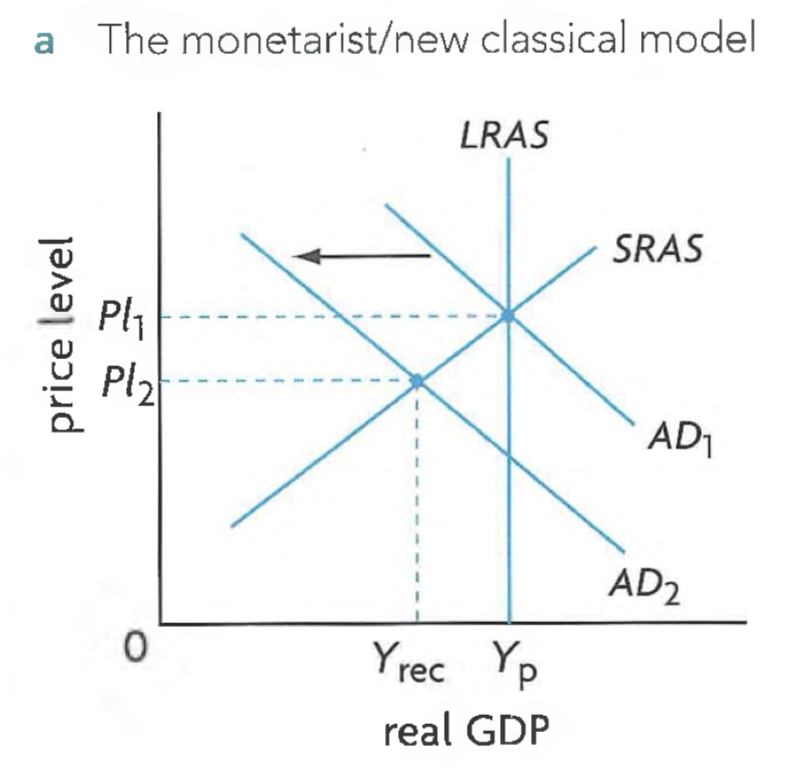
\includegraphics[width=0.3\linewidth]{Screenshot 2026-07-26 at 15.09.25.png}
    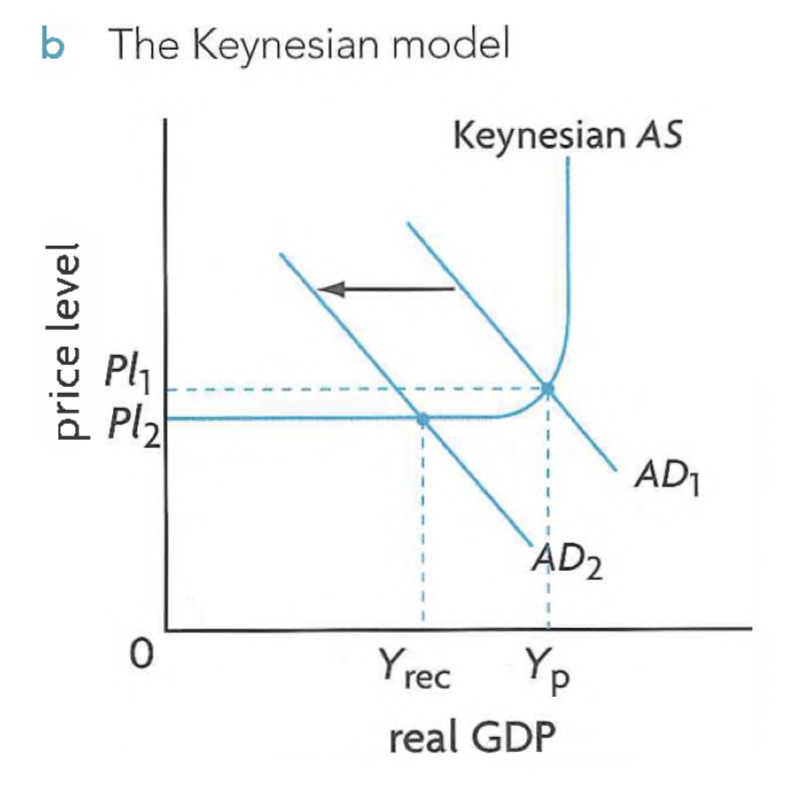
\includegraphics[width=0.3\linewidth]{Screenshot 2026-07-26 at 15.09.57.png}
  \end{center}
\end{itemize}
\textbf{The natural rate of unemployment} $=$ structural $+$ frictional $+$ seasonal unemployment. It is the unemployment that exists even when the economy produces at \textbf{full employment (potential) output}.
\begin{center}
  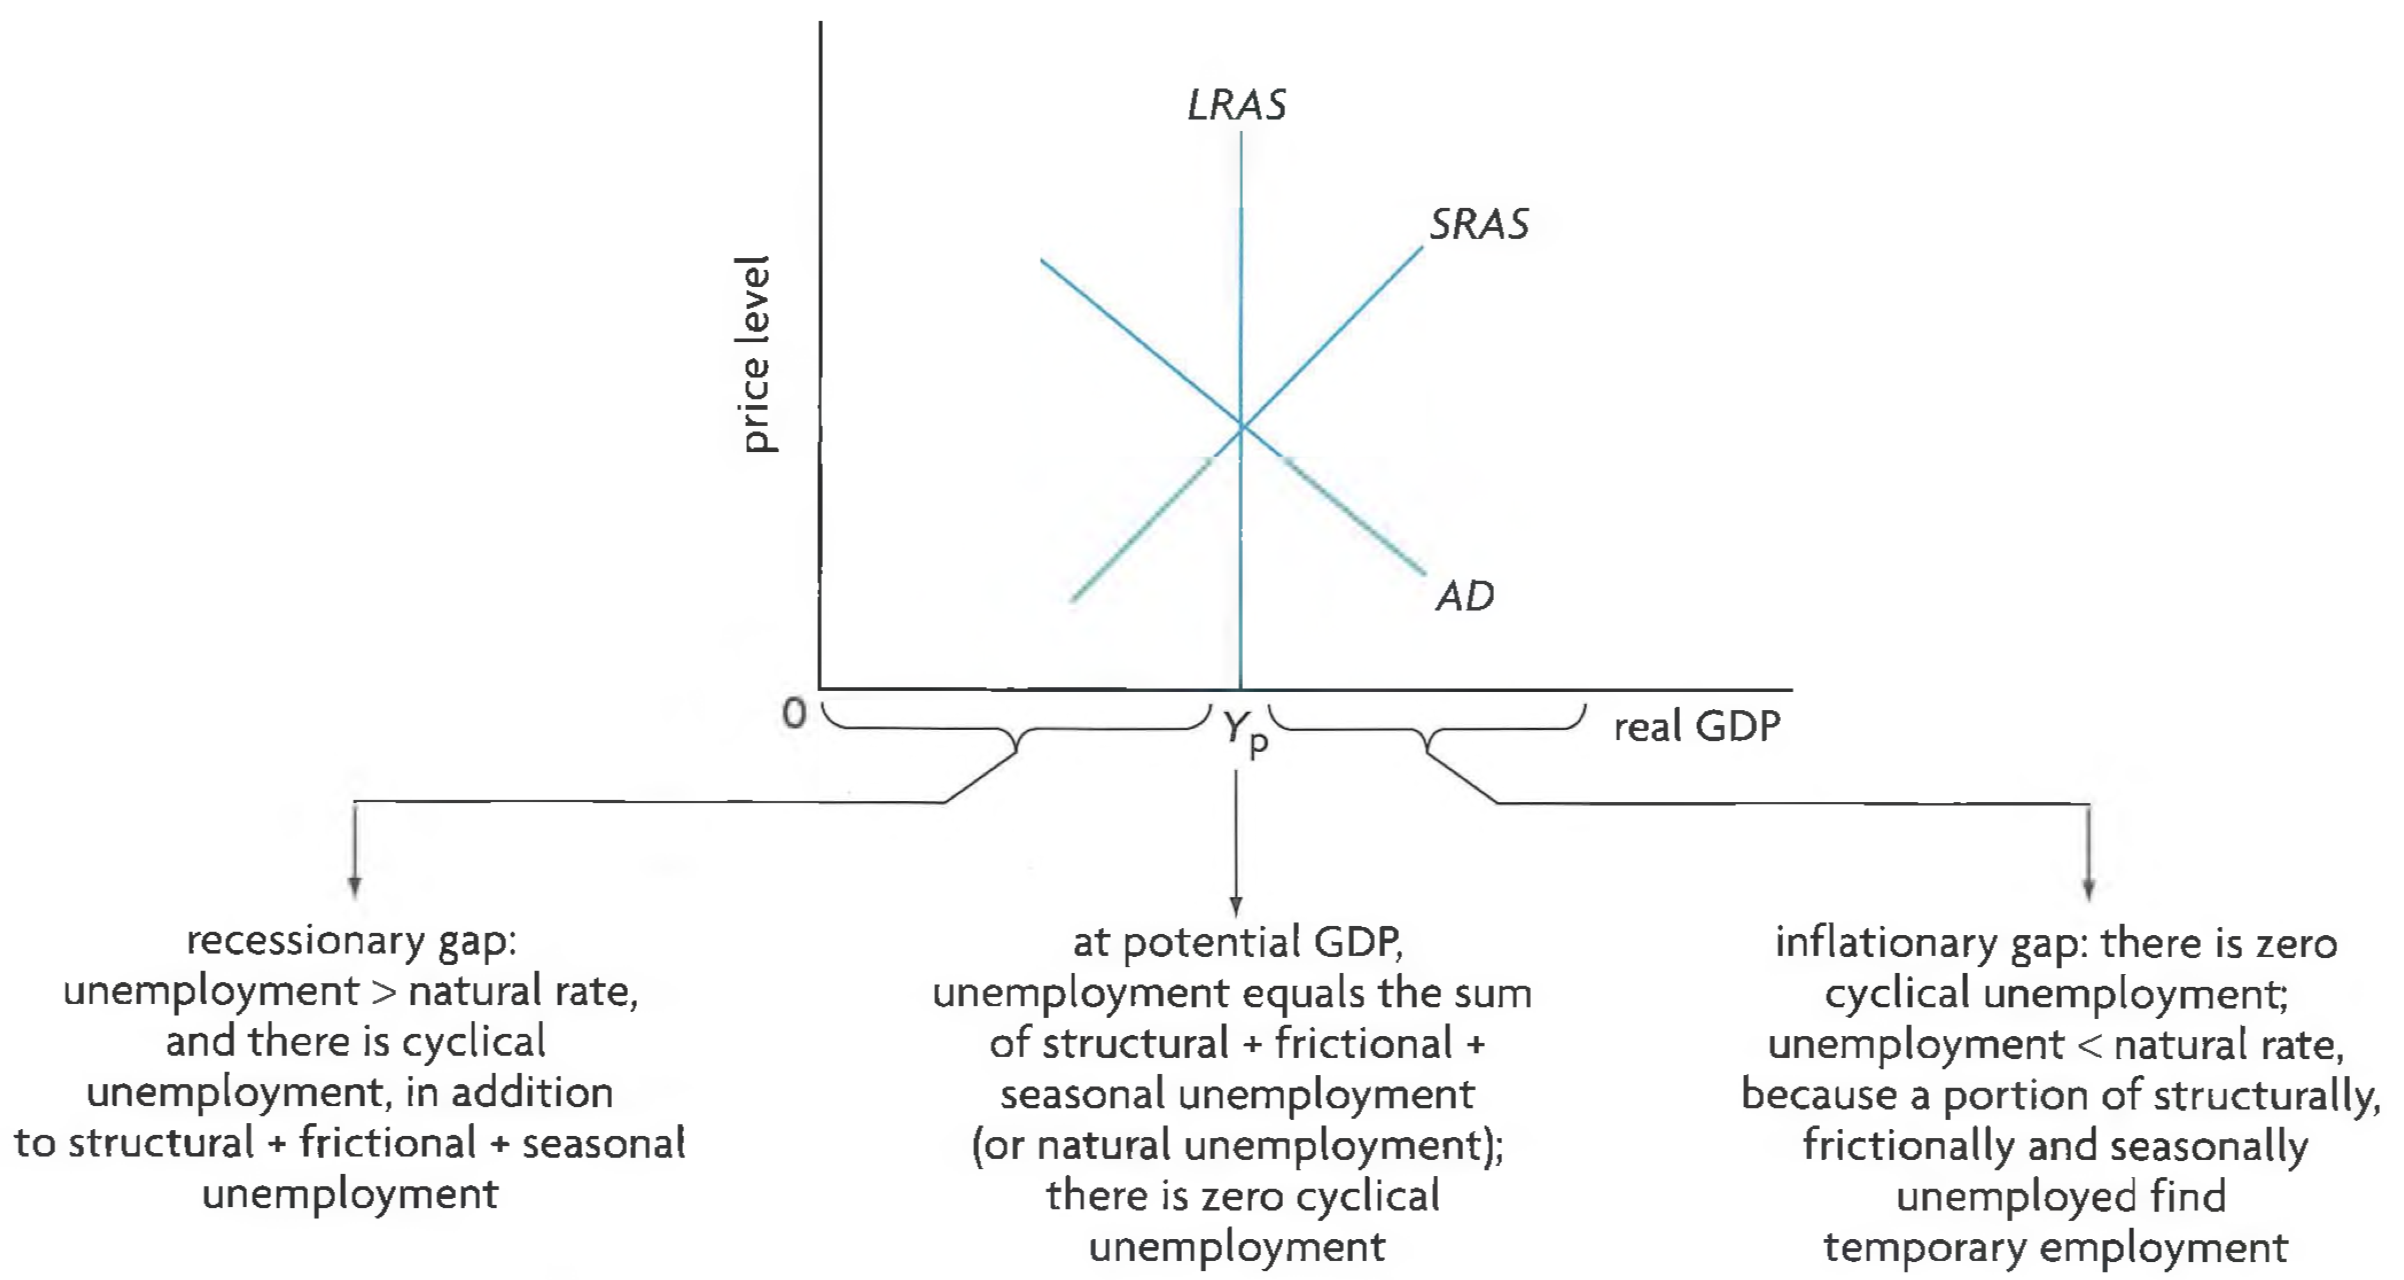
\includegraphics[width=0.9\linewidth]{Screenshot 2026-07-26 at 15.13.35.png}
\end{center}
\subsubsection*{Supplementary: Reservation wage (AP/Edexcel labour-market concept)}
\needbold{Reservation wage}: the \textbf{minimum wage rate} at which an individual worker is willing to accept a job offer and supply labour. Below this wage, the worker prefers non-market alternatives: leisure, household production, further education, or continued job search supported by unemployment benefits; at or above it, the worker enters employment.
\begin{itemize}
  \item \textbf{Individual and market supply}: at wages below the reservation wage, individual labour supply is zero. For the aggregate market, the reservation wage corresponds to the \textbf{vertical intercept of the labour supply curve}.
  \item \textbf{Determinants}:
  \begin{itemize}
    \item \textbf{Factors raising the reservation wage}: generous unemployment benefits or welfare safety nets (higher non-work income); greater family wealth; high search costs; high commuting or child-care costs.
    \item \textbf{Factors lowering the reservation wage}: expiry or reduction of unemployment benefits; lower household wealth; high cost of living; high job scarcity.
  \end{itemize}
  \item \textbf{Link to frictional unemployment}: unemployed workers accept the first wage offer that meets or exceeds their reservation wage. When reservation wages are high relative to prevailing wage distributions, search durations lengthen, increasing \textbf{frictional unemployment}. Policies that reduce unemployment benefit generosity lower reservation wages and speed up job acceptance (a market-based supply-side reform).
  \item \textbf{Link to labour force participation}: individuals whose reservation wages exceed all available wage offers drop out of the active labour force.
  \item \textbf{Policy implications}:
  \begin{itemize}
    \item \textbf{Minimum wage}: to be binding, a statutory minimum wage must exceed the reservation wage of marginal workers. If set moderately above monopsony wages, it can increase employment; if set far above productivity, it can price low-skilled workers out of work.
    \item \textbf{Labour income taxes}: taxes reduce net take-home pay, effectively requiring a higher gross wage to meet the worker's reservation threshold. Targeted tax credits (e.g.\ Earned Income Tax Credit) raise net pay and boost labour supply.
  \end{itemize}
\end{itemize}
\begin{center}
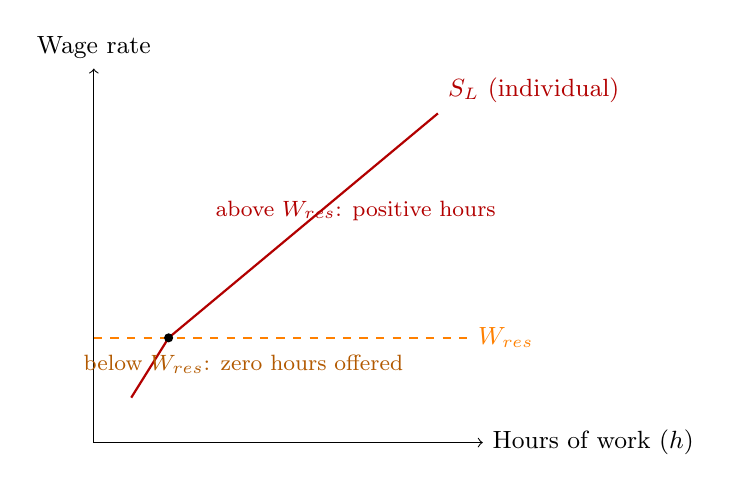
\begin{tikzpicture}[scale=0.95]
\draw[->] (0,0) -- (5.2,0) node[right, font=\small] {Hours of work ($h$)};
\draw[->] (0,0) -- (0,5.0) node[above, font=\small] {Wage rate};
% Reservation wage line
\draw[thick, orange, dashed] (0,1.4) -- (5.0,1.4) node[right, orange, font=\small] {$W_{res}$};
% Supply: zero below reservation, upward-sloping above (simple kinked curve)
\draw[thick, red!70!black] (0.5,0.6) -- (1.0,1.4);
\draw[thick, red!70!black] (1.0,1.4) -- (4.6,4.4) node[above right, red!70!black, font=\small] {$S_L$ (individual)};
\filldraw (1.0,1.4) circle (1.5pt);
% Labels
\node[font=\footnotesize, orange!70!black, align=center] at (2.0,1.05) {below $W_{res}$: zero hours offered};
\node[font=\footnotesize, red!70!black, align=center] at (3.5,3.1) {above $W_{res}$: positive hours};
\end{tikzpicture}
\end{center}
\subsection{Low and stable rate of inflation}
\needbold{Inflation}: sustained rise in general price level (an average of prices of goods and services in the entire economy).\\
\needbold{Deflation}: a sustained decrease in the general price level.
\needbold{Disinflation}: a decrease in the rate of inflation.\\
Measures of inflation and deflation are obtained by the use of price indices (CPI, PPI, RPI...), measure of average prices in one period relative to average prices in a reference period called a base period.\\
The \needbold{consumer price index (CPI)} is a measure of the cost of living for the typical household, and compares the value of a basket of goods and services in one year with the value of the same basket in a base year. Inflation (and deflation) are measured as a percentage change in the value of the basket from one year to another.
\[PI=\dfrac{\text{Value of basket in a specific year}}{\text{Value of the same basket in the base year}}\times 100\]
(Remember to consider weights for constructing PI if there exists such weights)
\[\Delta \% \text{Inflation / Deflation}=\dfrac{PI_2-PI_1}{PI_1}\times 100\]
\[\text{real income}=\dfrac{\text{nominal income}}{CPI}\times 100\]
Problems with CPI:
\begin{itemize}
  \item \textbf{Different rates of inflation for different income earners}: the CPI basket reflects the \textit{average} household, but consumption patterns vary by income level $\to$ different groups face different inflation rates.
  \item \textbf{Different rates of inflation by regional/cultural factors}: tastes and purchases vary by region and culture, so the CPI may not reflect specific groups' actual inflation.
  \item \textbf{Consumer substitutions when relative prices change}: as some goods become cheaper/more expensive, consumers substitute, but fixed weights in the basket cannot capture this $\to$ CPI usually \textbf{overstates} inflation.
  \item \textbf{Increasing use of discount stores and sales}: consumers buy at lower prices than those used in CPI calculations $\to$ CPI overstates inflation.
  \item \textbf{Introduction of new products}: a fixed basket cannot account for new products (e.g.\ Netflix replacing DVDs) or products becoming obsolete.
  \item \textbf{Changes in product quality}: the CPI cannot account for quality improvements over time.
  \item \textbf{International comparisons}: CPIs differ across countries in basket composition, weights and calc methods $\to$ limited comparability. The EU has devised the \textbf{Harmonised Index of Consumer Prices (HICP)} to ensure consistency.
  \item \textbf{Comparability over time}: countries periodically revise baskets and base years (roughly every 10 years; weights may change annually). Price indices are comparable over short periods, but comparability diminishes over longer periods due to cumulative basket changes.
\end{itemize}
Note that there are G\&S with highly volatile prices due to wide swings in supply and demand, which, if included in the calculation of CPI, could cause misleading impressions regarding rate of inflation. In order to tackle this problem, a CPI without these G\&S is constructed to represent the core rate of inflation (excluding the impact of those goods that have high price volatility)\\\\
\subsubsection*{Comparing the CPI with the GDP deflator (supplementary)}
Inflation can also be measured with the \textbf{GDP deflator} ($\text{Nominal GDP}/\text{Real GDP} \times 100$). The two indices usually move in the same direction but are \textbf{not identical}:
\begin{itemize}
  \item The \textbf{CPI} uses a \textbf{fixed basket} of goods and services (valued at prices that change over time); the \textbf{GDP deflator} uses \textbf{actual output} (which changes over time) valued at fixed base-year prices.
  \item Because the deflator is not based on a fixed basket, it \textbf{does not suffer from the CPI's substitution/new-product/quality biases} --- it is a more accurate measure of the \textit{average price level} of the whole economy.
  \item Yet the \textbf{CPI is preferred} for cost-of-living purposes because:
  \begin{itemize}
    \item the GDP deflator includes goods \textbf{irrelevant to consumers} (exports, capital goods, government purchases) and \textbf{excludes imports} (which consumers do buy, e.g.\ imported oil);
    \item a fixed basket with \textbf{weights based on the typical household's budget} lets us measure price changes relevant to households, which the deflator's GDP weights do not;
  \end{itemize}
  \item In short: the \textbf{CPI measures changes in the cost of living}; the \textbf{GDP deflator measures changes in average prices for the economy as a whole}. Governments and central banks use the CPI to adjust nominal incomes (wages, pensions, welfare) and to guide monetary policy.
\end{itemize}
Causes of inflation:
\begin{itemize}
  \item \needbold{Demand-pull inflation}: caused by increase in AD. Involves an excess of aggregate demand over aggregate supply at the full employment level of output,
  \begin{center}
    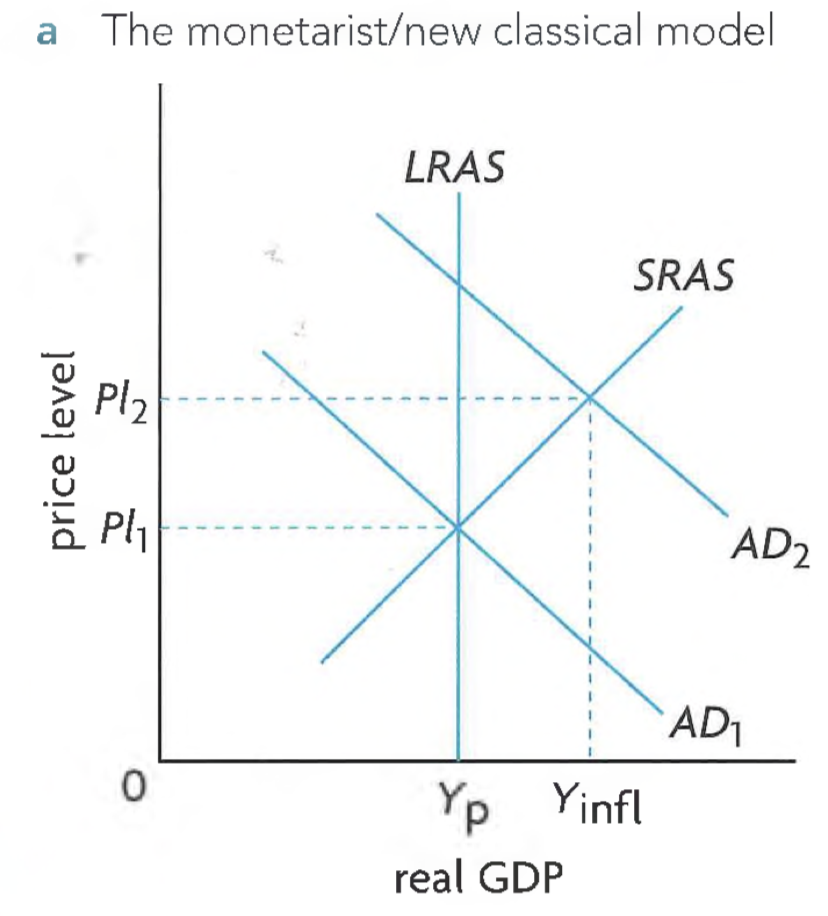
\includegraphics[width=0.35\linewidth]{Screenshot 2026-07-26 at 15.34.12.png}
    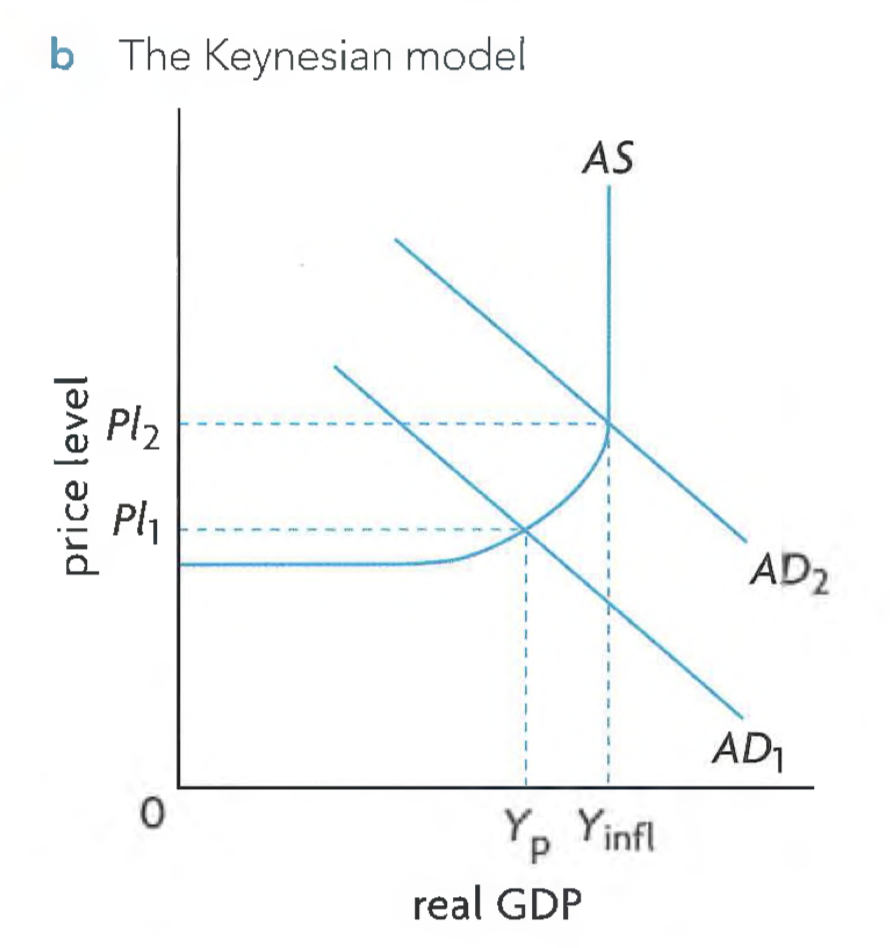
\includegraphics[width=0.37\linewidth]{Screenshot 2026-07-26 at 15.34.29.png}
  \end{center}
  \item \needbold{Cost-push inflation} / \needbold{stagflation}: increases in costs of production or supply-side shocks, decrease in AS, not desirable.
  \begin{center}
    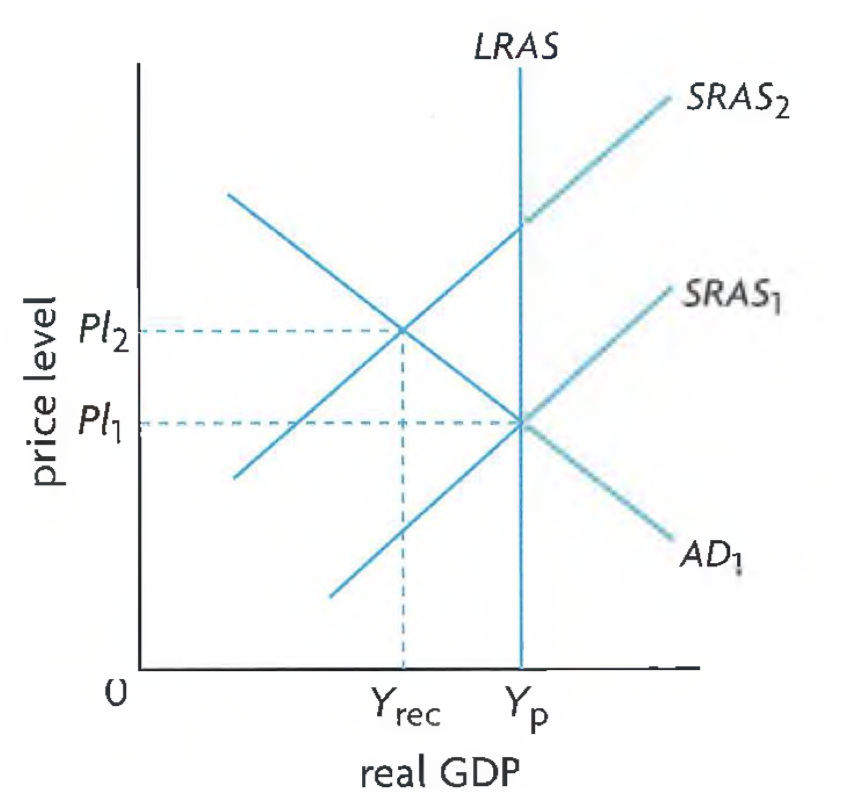
\includegraphics[width=0.35\linewidth]{Screenshot 2026-07-26 at 15.37.23.png}\\
    Note that there's no Keynesian interpretation of cost-push inflation.
  \end{center}
\end{itemize}
\needbold{Purchasing power}: the quantity of goods and services that can be bought with money.\\
\% change in real income = \% change in nominal income - \% change in price level / rate of inflation.\\
Therefore, if nominal income stays constant / increases more slowly than rate of inflation, then your purchasing power decreases.\\\\
Costs of inflation:
\begin{itemize}
  \item \textbf{Redistribution effects} --- inflation redistributes income and purchasing power:
  \begin{itemize}
    \item \textit{Groups that lose}: people on \textbf{fixed incomes/wages} (wage contracts, pensions, rent, welfare payments); people whose incomes rise \textbf{slower than inflation}; \textbf{holders of cash} (real value falls); \textbf{savers} (if interest $<$ inflation, real value of savings falls); \textbf{lenders/creditors} (repaid in money worth less than when lent).
    \item \textit{Groups that gain}: \textbf{borrowers/debtors} (repay with money worth less); \textbf{payers of fixed incomes} (firms, governments, landlords --- real value of payments falls).
  \end{itemize}
  \item \textbf{Uncertainty}: inability to predict future price levels $\to$ firms cannot forecast costs/revenues accurately $\to$ \textbf{less investment} $\to$ lower economic growth.
  \item \textbf{Lower saving}: savers lose when interest $<$ inflation $\to$ less incentive to save; people spend now to avoid higher future prices $\to$ further reduces saving.
  \item \textbf{Loss of international competitiveness}: domestic prices rise faster than trading partners $\to$ exports more expensive, imports cheaper $\to$ exports fall, imports rise $\to$ worsens balance of payments.
  \item \textbf{Lower economic growth}: uncertainty $\to$ less investment; lower saving $\to$ less funds for investment; lower net exports --- all reduce AD $\to$ lower real GDP.
  \item \textbf{Misallocation of resources}: rapid price rises distort the \textbf{signalling and incentive functions} of the price mechanism (prices don't rise uniformly) $\to$ allocative inefficiency increases.
  \item \textbf{Social/personal costs unequally distributed}: low-income groups are hit hardest (pensioners, unemployed, workers with slow-rising wages); they cannot protect savings with assets like real estate or gold; food and energy price rises cut deeply into their incomes.
\end{itemize}
\textbf{Hyperinflation}: defined as price level increasing $>50\%$ per month (can reach millions of percent per year). Caused by governments \textbf{printing money} (massive increases in money supply). Consequences:
\begin{itemize}
  \item Consumers rush to spend before prices rise further $\to$ \textbf{demand-pull} inflation.
  \item Workers demand higher wages $\to$ \textbf{cost-push} inflation $\to$ \textbf{inflationary spiral}.
  \item Businesses stop productive investment; shift to assets holding value (gold, real estate); firms withhold goods to sell later at higher prices.
  \item Creditors suffer massive losses; at the extreme, \textbf{money loses all value} $\to$ people resort to \textbf{barter}; economic activity is massively disrupted; political and social unrest may follow.
\end{itemize}
\textbf{Appropriate rate of inflation}: most governments prefer a \textbf{low and stable rate of $\sim$2--3\% per year}.\\\\
Why deflation is rare?
\begin{itemize}
  \item Wages of workers do not ordinarily fall.
  \item Large oligopolistic firms may fear price wars. 
  \item ......
\end{itemize}
Causes of deflation:
\begin{itemize}
  \item Decrease in AD, 'bad' deflation
  \item Increase in AS, 'good' deflation
\end{itemize}
\begin{center}
  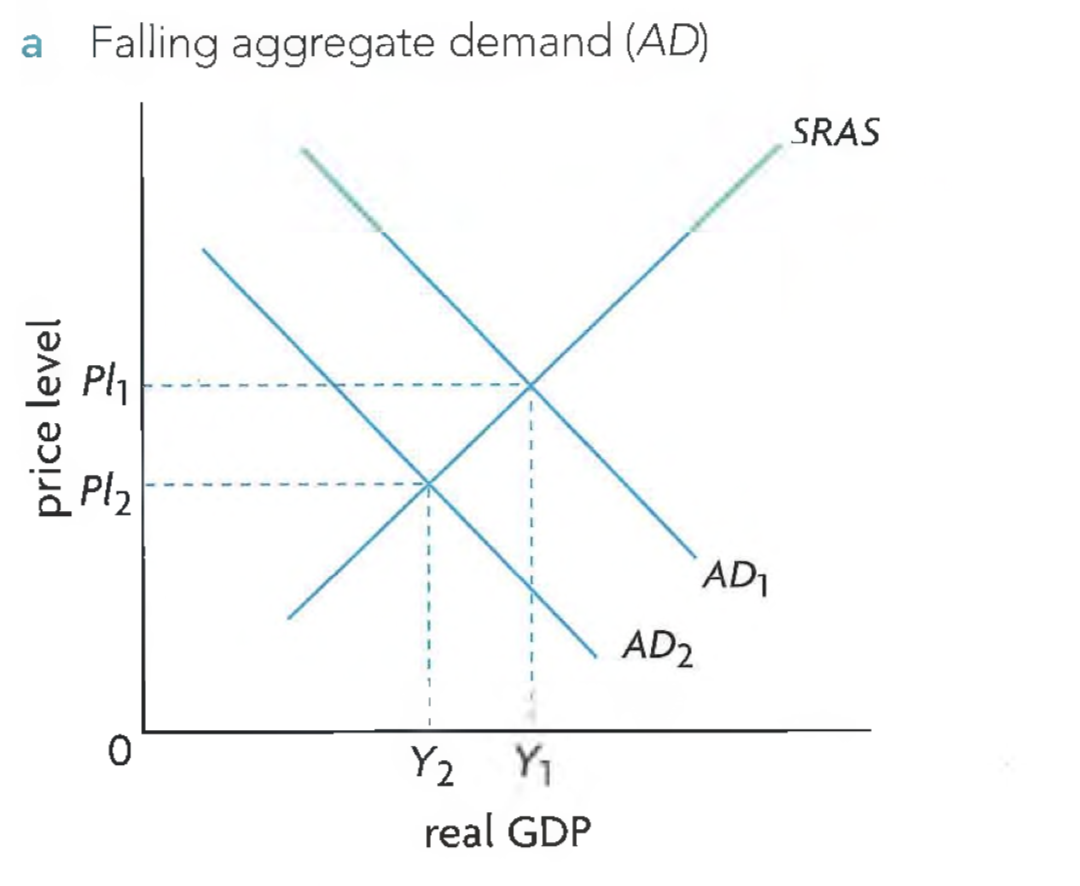
\includegraphics[width=0.4\linewidth]{Screenshot 2026-07-26 at 15.50.44.png}
  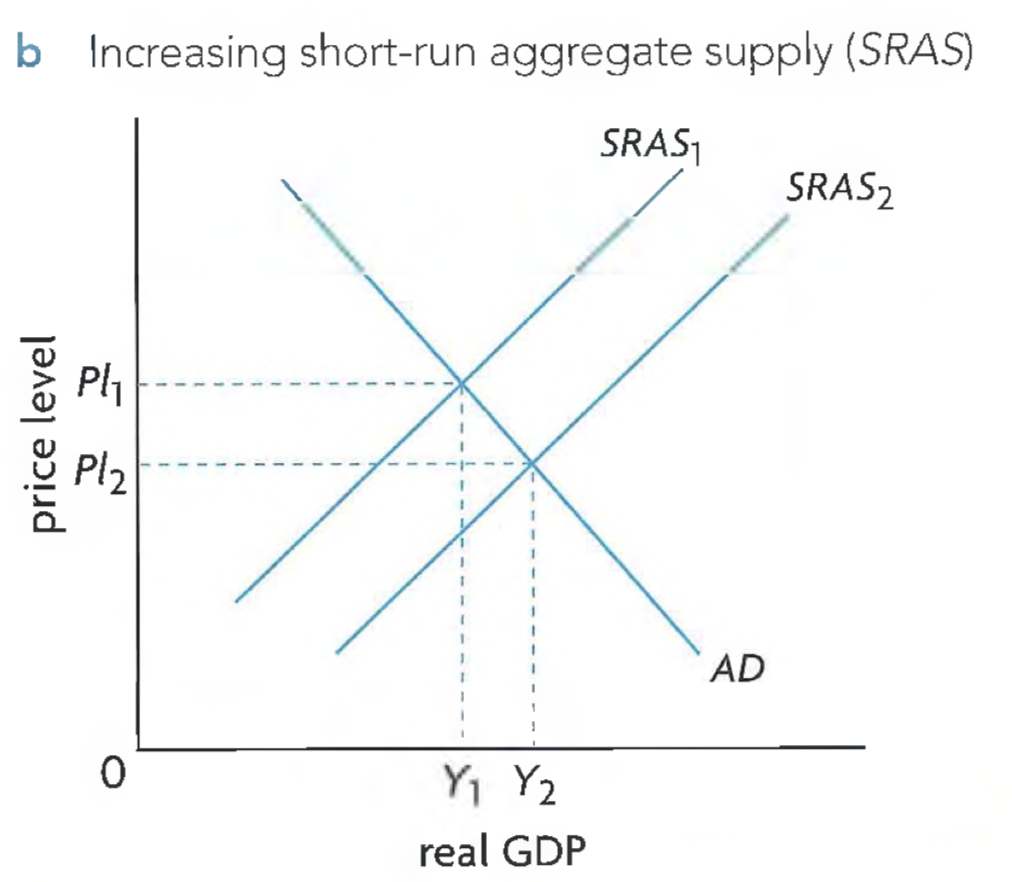
\includegraphics[width=0.38\linewidth]{Screenshot 2026-07-26 at 15.50.58.png}
\end{center}
Costs of deflation:
\begin{itemize}
  \item \textbf{Redistribution effects} (opposite of inflation): people on \textbf{fixed incomes}, \textbf{cash holders}, \textbf{savers} and \textbf{lenders} \textit{gain} (real value of holdings rises); \textbf{borrowers/debtors} and \textbf{payers of fixed incomes} \textit{lose} (must repay/pay out sums with increasing real value).
  \item \textbf{Increase in the real value of debt}: as the price level falls, the purchasing power of owed money increases $\to$ debts become heavier in real terms.
  \item \textbf{Uncertainty}: firms cannot forecast costs/revenues due to declining price levels $\to$ less investment.
  \item \textbf{Deferred consumption}: consumers \textbf{postpone spending} expecting further price falls; borrowing is discouraged (real value of debt rises) $\to$ consumer and business spending fall $\to$ AD falls $\to$ lower real GDP, higher cyclical unemployment, further price falls $\to$ further spending postponement $\to$ \textbf{deflationary spiral}.
  \item \textbf{Risk of bankruptcies and financial crisis}: falling incomes + rising real debt $\to$ firms and consumers unable to repay $\to$ bankruptcies; if widespread, banks/financial institutions are threatened $\to$ risk of major \textbf{financial crisis}.
  \item \textbf{Inefficient resource allocation}: prices do not fall uniformly $\to$ distorted price signals and incentives $\to$ resource misallocation.
  \item \textbf{Policy ineffectiveness}: once deflationary expectations set in, consumers are hard to change; more importantly, \textbf{expansionary monetary policy} (lowering interest rates) becomes ineffective once rates approach \textbf{zero} (the ``zero lower bound'').
\end{itemize}
\textbf{One positive effect}: deflation improves \textbf{international competitiveness} --- lower domestic prices $\to$ exports increase, imports decrease $\to$ net exports ($X - M$) rise, putting upward pressure on AD and real GDP. 
\subsection{Exploring the relationship between unemployment and inflation}
\textbf{Okun's Misery Index} = unemployment rate + inflation rate. A rough measure of economic well-being, but it does not distinguish which causes more harm.\\\\
\subsubsection*{Okun's Law}
\needbold{Okun's Law} (Arthur Okun, 1962; same economist as the Misery Index) is an empirical relationship between the \textbf{unemployment rate} and the \textbf{output gap} (real GDP relative to potential output):
\begin{itemize}
  \item \textbf{Output-gap version} (the usual AP rule of thumb):
  \[\text{Output gap} \approx -2 \times (u - u^*)\]
  where $u$ is the actual unemployment rate and $u^*$ is the natural rate. Each \textbf{1 percentage point} of unemployment \textbf{above the natural rate} corresponds to real GDP about \textbf{2\% below potential output}. (Negative output gap $=$ recessionary/deflationary gap; positive $=$ inflationary gap.)
  \item \textbf{Growth version} (predicting unemployment changes from GDP growth):
  \[\Delta u \approx -\dfrac{1}{2}\left(\text{real GDP growth} - \text{trend growth}\right)\]
  i.e.\ if real GDP grows about \textbf{2 percentage points above its trend rate for a year}, the unemployment rate falls by about \textbf{1 percentage point}.
  \item \textbf{Worked example}: natural rate $u^* = 5\%$, actual unemployment $u = 7\%$ $\Rightarrow$ output gap $\approx -2 \times (7\% - 5\%) = -4\%$, so real GDP is about 4\% below potential.
\end{itemize}
\textbf{Why it matters}:
\begin{itemize}
  \item \textbf{Quantifies the cost of unemployment}: every extra point of cyclical unemployment means roughly 2\% of output (income, tax revenue, living standards) is lost.
  \item \textbf{Links two macroeconomic objectives}: low unemployment and economic growth are two sides of the same coin --- closing a recessionary gap (raising real GDP to potential) simultaneously reduces cyclical unemployment toward the natural rate.
  \item \textbf{Only cyclical unemployment matters}: the law works through the output gap, so it applies to \textbf{cyclical} (demand-deficient) unemployment, not structural, frictional or seasonal unemployment --- those can change with $u^*$ itself (e.g.\ labour market reforms shift the natural rate).
  \item It also highlights \textbf{reverse causality}: low growth raises unemployment, but high unemployment also lowers growth (wasted resources, hysteresis), so the relationship is not a strict one-way law.
\end{itemize}
\textbf{Caveats}: it is an \textbf{empirical rule of thumb, not a physical law} --- the coefficient varies across countries and time periods (estimates commonly range from about 1.5 to 3, and the ``2-for-1'' figure is the standard AP convention); it is less reliable at very low unemployment; and it cannot tell us \textit{why} unemployment deviates from the natural rate.
\\\\
Economically, it is hard to generalise which is more costly --- it depends on circumstances (how high each rate is, the economy's structure). However, well-being studies find that \textbf{unemployment has a far stronger negative impact}. Unemployment also harms not just the unemployed but their families and communities. This explains why governments often tolerate moderate inflation to avoid high unemployment.\\\\
There exists a \textbf{conflict between low unemployment and low inflation}: as AD increases and the economy approaches potential output, cyclical unemployment falls but the price level begins to rise (due to resource bottlenecks and higher wages). Beyond potential output (inflationary gap), unemployment falls below the natural rate but inflation accelerates rapidly --- making it difficult to achieve both low inflation and low unemployment simultaneously.
\subsubsection*{Tradeoff between unemployment and inflation}
The Phillips curve: demonstrates the long-term negative relationship between unemployment and inflation. (With every increase in aggregate demand, we have an increase in the price level and a fall in unemployment.) Each point on the Phillips curve can be thought as an intersection of SRAS curve and a changing AD curve.\\
Shifts in AD is represented as a movement along the Phillips curve (increase in AD signifies higher price level and lower unemployment). Shifts in AS in represented as a shift of the Phillips curve. (Decrease in AS signifies increase in both unemployment and price level) This applies to short-run Phillips curve only.
\begin{center}
  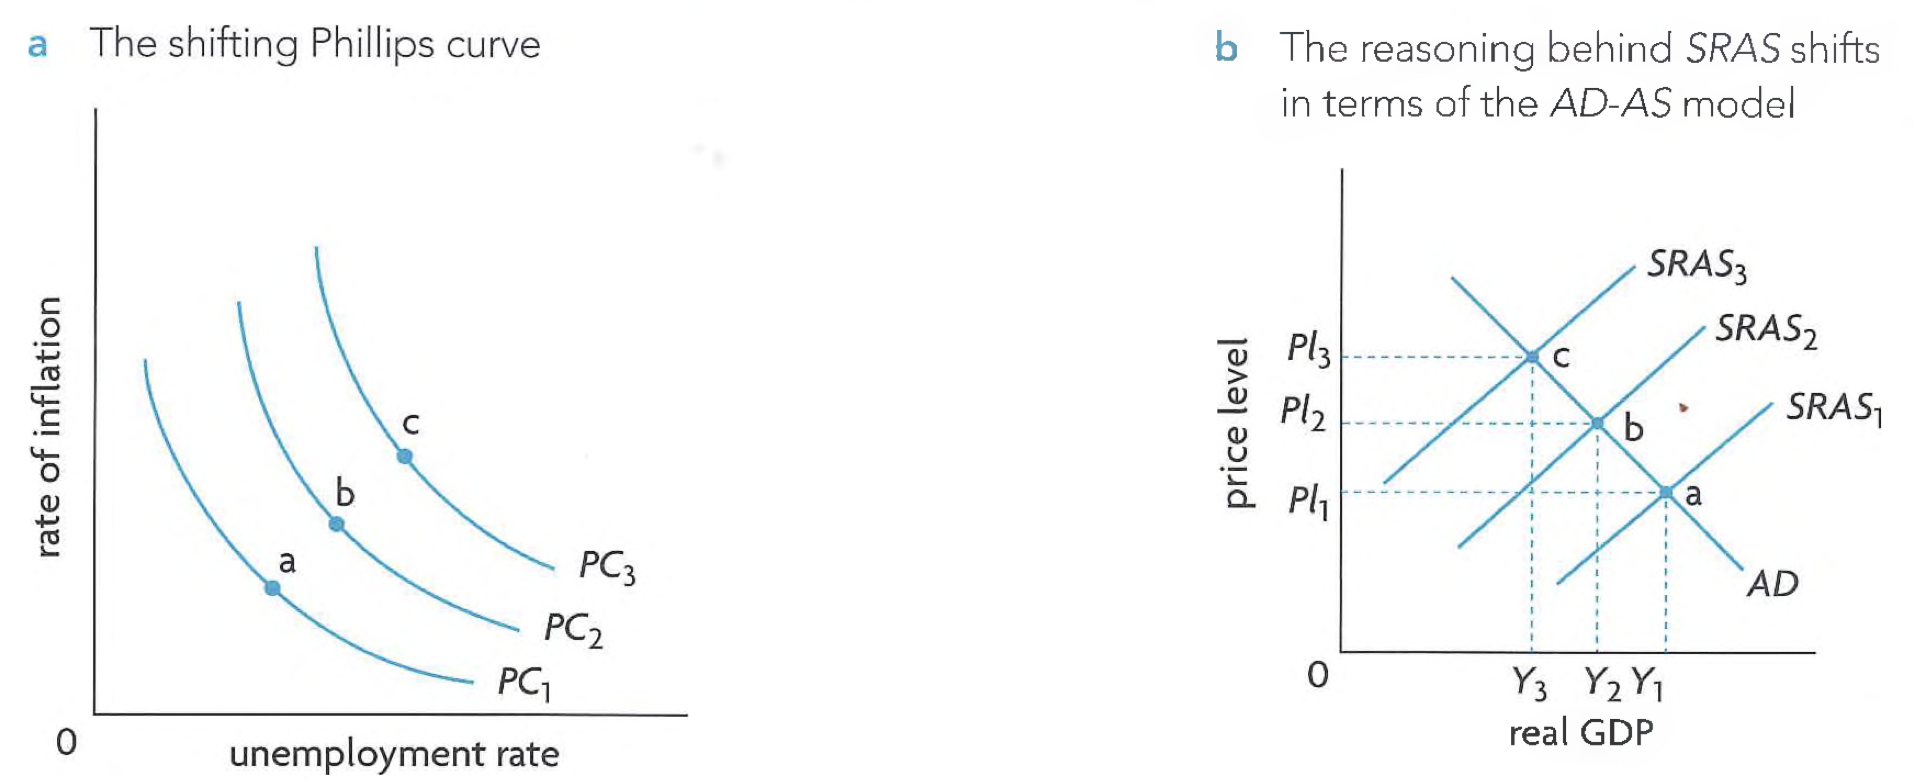
\includegraphics[width=0.8\linewidth]{Screenshot 2026-07-26 at 19.09.32.png}
\end{center}
For long-run Phillips curve, it's vertical at the level of full employment / when unemployment rate = natural rate of unemployment.
\begin{itemize}
  \item In the \textbf{short run}, an increase in AD moves the economy along the SRPC: lower unemployment, higher inflation (wages are constant $\to$ firm profitability rises $\to$ more output, less unemployment).
  \item In the \textbf{long run}, wages rise to catch up with the higher price level $\to$ SRAS shifts left $\to$ real GDP returns to potential, unemployment returns to the natural rate, but inflation is now permanently higher. The economy has shifted to a \textbf{new SRPC} further right.
  \item The LRPC connecting these points is \textbf{vertical}: in the long run, unemployment is \textbf{independent} of the inflation rate. Increases in AD only cause inflation, without changing real output or unemployment.
\end{itemize}
\textbf{Policy implications}:
\begin{itemize}
  \item \textbf{Keynesians} prefer the \textbf{SRPC}: demand-side policies can trade off inflation and unemployment.
  \item \textbf{Monetarist/new classical} economists prefer the \textbf{LRPC}: expansionary demand-side policies only cause inflation; they advocate \textbf{supply-side policies} to shift LRAS/LRPC rightward.
\end{itemize}
\section{Macroeconomic objectives II}
\subsection{Economic growth}
\needbold{Economic growth} refers to an increase in real GDP, or the real quantity of goods and services produced over a period of time (typically a year), and is usually expressed as a percentage change in GDP (per capita) over a period of time.
\[\Delta \%\text{Real GDP}=\dfrac{Y_2-Y_1}{Y_1}\times 100\]
If real GDP is growing faster than the population, then the amount of real GDP that corresponds to each person on average increases, resulting in positive growth in real GDP per capita.\\
\% Change in real GDP per capita = \% Change in real GDP - \% Change in population
\subsubsection*{Short-term vs Long-term growth}
In the AD-AS model, economic growth occurs as a result of
\begin{itemize}
  \item increase in AD, short-term growth (more often)
  \item increase in SRAS, short-term growth
  \item increase in LRAS / Keynesian AS, long-term growth
\end{itemize}
Short-term growth is shown in the expansion phase of the business cycle, when real GDP is increasing over time, though this is followed by a contraction, or a period of decreasing real GDP. The contraction illustrates situations where there is negative growth. 
The business cycle diagram, showing an upward-sloping, long-term growth trend, indicates that the economy's real GDP is growing over time. (i.e, long-term growth)\\\\
It could also be interpreted using the PPC: 
\begin{itemize}
  \item Short-term growth: growth in actual output (movement of point inside the area bounded by the curve) by improving efficiency or reducing unemployment
  \item Long-term growth: outward shifts in PPC \emph{per se}
  \begin{itemize}
    \item Increases in the quantity of resources (FoPs) in the economy
    \item Improvements in the quality of resources (e.g. education / physical capital)
    \item Efforts must be made to keep unemployment low and reduce inefficiencies
  \end{itemize} 
\end{itemize}
\subsubsection*{Why economic growth happens}
Different types of capital:
\begin{itemize}
  \item Physical capital: results from investments to produce man-made products
  \item Human capital: skills, abilities, knowledge, levels of health of workers.
  \item Natural capital: everything that falls within 'land', but the overall amount is changing
\end{itemize}
Investments are crucial to building all types of capitals:
\begin{itemize}
  \item \textbf{Physical capital, technology and growth}: increases in quantity (more machines, roads, ports) and improvements in quality (technological advances \textbf{embodied} in new capital goods, e.g.\ faster computers) are among the most important sources of long-term growth.
  \item \textbf{Human capital and growth}: increases in \textit{quantity} of labour are less important (many countries have unemployment/underemployment); improvements in \textit{quality} (skills, knowledge, health via education, training, health care, sanitation, clean water) are far more important --- a skilled, healthy worker produces more output.
  \item \textbf{Natural capital and growth}:
  \begin{itemize}
    \item \textbf{Marketable commodities}: can contribute to growth but are \textbf{not essential}.
    \item \textbf{Common pool resources}: \textbf{important} for long-term growth. Environmental destruction reduces output directly (poorer soils, depleted fisheries) and indirectly (pollution damages worker health $\to$ lower human capital). Continued growth requires \textbf{investment in natural capital}.
  \end{itemize}
\end{itemize}
\subsubsection*{Productivity as a source of economic growth}
\textbf{Productivity:} output produced per hour of work (measured as real GDP $\div$ total hours worked). \\Improvements in productivity mean each hour of work produces more output $\to$ economic growth. Factors causing productivity improvements are the same as those driving long-term growth:
\begin{itemize}
  \item increases in quantity and quality of \textbf{physical capital} (investment + technology)
  \item improvements in quality of \textbf{labour} (investment in human capital)
  \item maintenance/improvement of \textbf{ecological resources} (investment in natural capital)
\end{itemize}
Productivity improvements cause \textbf{rightward shifts of LRAS/Keynesian AS} curves and \textbf{outward shifts of the PPC}.
\subsubsection*{Consequences of economic growth}
\begin{itemize}
  \item Living standards (or standards of living) refer to levels of income, wealth and consumption of goods and services, including health care and education. Reflected by GDP per capita.
  \begin{itemize}
    \item Redistribution of income
    \item Household spending
    \item The share of income controlled by women
    \item Government spending on merit goods
    \item Contributions by non-governmental organizations
  \end{itemize}
  While EG offers the potential to achieve improvements in standards of living, these improvements o not occur automatically as a result of EG but require appropriate policies to make effective use of the resources growth makes available.
  \item Environmental consequences: rapid growth often leads to \textbf{unsustainable resource use}. Many governments follow ``\textbf{grow now, clean up later}'', but this is flawed because:
\begin{itemize}
  \item Some environmental damage is \textbf{irreversible} (lost biodiversity, pollution-related deaths).
  \item It justifies government \textbf{inaction} --- environmental recovery does not happen automatically with higher incomes.
  \item It is not growth \textit{per se} that harms the environment, but \textbf{how} growth is pursued.
  \item Growth based on unsustainable resource use may \textbf{threaten future growth} itself.
\end{itemize}
Growth and sustainability \textbf{can be pursued together} under certain conditions:
\begin{itemize}
  \item Market-based policies that \textbf{internalize externalities} (carbon taxes, tradable permits) gives incentives for sustainable use and green technology.
  \item Environmental regulations encouraging \textbf{pollution-free technological change}.
  \item Greater emphasis on \textbf{human capital} (pollution-free) over physical capital.
  \item \textbf{Green investments}: public transport, building insulation, clean technology R\&D.
  \item Structural shifts toward \textbf{services} (less polluting) plus investment in resource protection.
\end{itemize}
However, even under ideal conditions there is a \textbf{maximum sustainable rate of growth}: pursuit of sustainability uses some resources (anti-pollution controls, regulation costs) representing an opportunity cost in terms of slightly lower growth --- but this only affects a portion of very high growth rates.
  \item Income distribution: the relationship between GDP per capita growth and income distribution are \textbf{inconclusive}. Yet income inequalities have been \textbf{widening globally}. Major causes:
\begin{itemize}
  \item \textbf{Market-based supply-side policies} (privatisation, deregulation).
  \item \textbf{Economic/trade liberalisation} $\to$ winners (skilled, mobile) vs.\ losers (unskilled, isolated, government-sector job losses).
  \item \textbf{Inappropriate government policies} in developing countries: capital-using technologies despite abundant labour; low investment in human capital; infrastructure concentrated in urban/formal sectors while rural areas and slums are neglected.
\end{itemize}
\end{itemize}
\subsubsection*{Impact of economic growth on unemployment and inflation (supplementary)}
\textbf{Growth and unemployment}:
\begin{itemize}
  \item \textbf{Short-term growth} (expansionary phase of the business cycle) reduces \textbf{cyclical unemployment}. If AD keeps rising beyond full employment (inflationary gap), unemployment can even fall \textbf{below} the natural rate --- but only temporarily, since contractionary policies (or self-correction) bring it back.
  \item \textbf{Long-term growth} (increases in potential output, rightward shifts of LRAS/Keynesian AS) can reduce \textbf{natural} and especially \textbf{structural} unemployment (via supply-side factors: more/better resources, technology). But \textbf{not all growth lowers unemployment}: growth driven by technological change may \textit{increase} structural unemployment (skills become obsolete), and capital-intensive technologies in developing countries may raise unemployment.
\end{itemize}
\textbf{Growth and inflation}:
\begin{itemize}
  \item In the \textbf{Keynesian} model, growth from AD increases is non-inflationary while there is spare capacity (horizontal AS); as real GDP approaches potential output, resource bottlenecks push prices up, and beyond potential output further AD growth is highly inflationary.
  \item In the \textbf{monetarist/new classical} model, an AD increase \textit{always} raises the price level in the short run, and in the long run only raises the price level.
  \item Both models agree: \textbf{long-term growth} (increases in potential output) \textbf{reduces inflationary pressure} --- AD growth matched by LRAS/AS growth does not raise prices.
  \item The relationship also runs the other way: unemployment and inflation affect growth (unemployment wastes resources; high inflation discourages investment and net exports).
\end{itemize}
\begin{center}
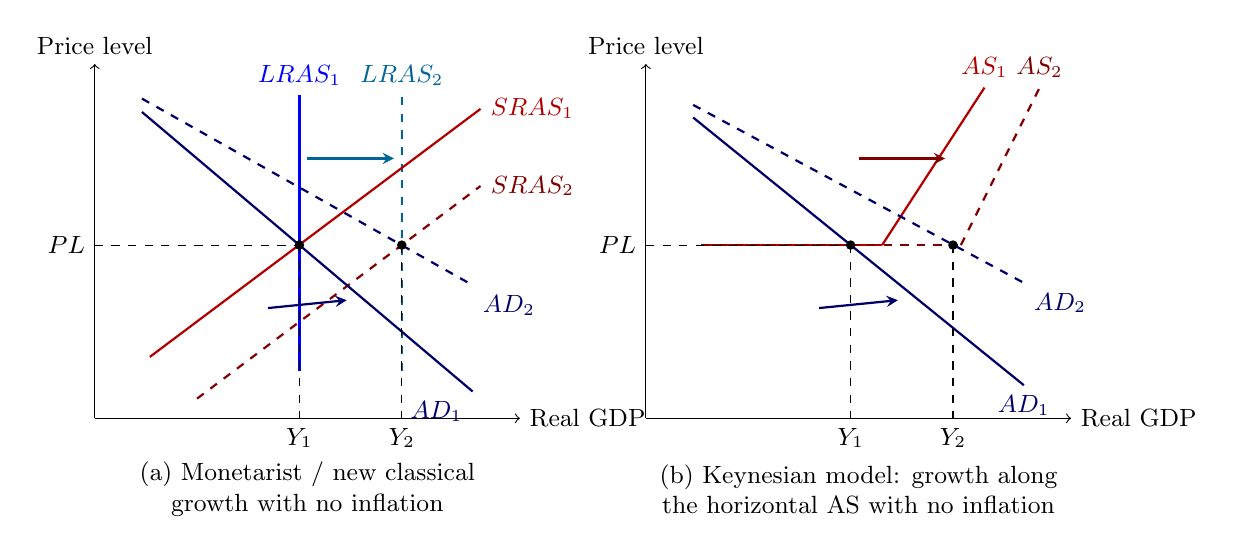
\begin{tikzpicture}[scale=1.0]
% (a) Monetarist / new classical model
\begin{scope}
\draw[->] (0,0) -- (5.4,0) node[right, font=\small] {Real GDP};
\draw[->] (0,0) -- (0,4.5) node[above, font=\small] {Price level};
\draw[thick, blue] (2.6,0.6) -- (2.6,4.1) node[above, blue, font=\small] {$LRAS_1$};
\draw[thick, blue!60!green, dashed] (3.9,0.6) -- (3.9,4.1) node[above, blue!60!green, font=\small] {$LRAS_2$};
\draw[thick, red!70!black] (0.7,0.78) -- (4.9,3.93) node[right, red!70!black, font=\small] {$SRAS_1$};
\draw[thick, red!50!black, dashed] (1.3,0.25) -- (4.9,2.95) node[right, red!50!black, font=\small] {$SRAS_2$};
\draw[thick, blue!40!black] (0.6,3.89) -- (4.8,0.34) node[below left, blue!40!black, font=\small] {$AD_1$};
\draw[thick, blue!40!black, dashed] (0.6,4.06) -- (4.8,1.69) node[below right, blue!40!black, font=\small] {$AD_2$};
\filldraw (2.6,2.2) circle (1.5pt);
\filldraw (3.9,2.2) circle (1.5pt);
\draw[dashed] (2.6,2.2) -- (2.6,0) node[below, font=\small] {$Y_1$};
\draw[dashed] (3.9,2.2) -- (3.9,0) node[below, font=\small] {$Y_2$};
\draw[dashed] (0,2.2) -- (2.6,2.2);
\node[left, font=\small] at (0,2.2) {$PL$};
\draw[->, >=stealth, thick, blue!60!green] (2.7,3.3) -- (3.8,3.3);
\draw[->, >=stealth, thick, blue!40!black] (2.2,1.4) -- (3.2,1.5);
\node[font=\small, align=center] at (2.7,-0.9) {(a) Monetarist / new classical\\ growth with no inflation};
\end{scope}
% (b) Keynesian model
\begin{scope}[xshift=7.0cm]
\draw[->] (0,0) -- (5.4,0) node[right, font=\small] {Real GDP};
\draw[->] (0,0) -- (0,4.5) node[above, font=\small] {Price level};
\draw[thick, red!70!black] (0.7,2.2) -- (3.0,2.2);
\draw[thick, red!70!black] (3.0,2.2) -- (4.3,4.2) node[above, red!70!black, font=\small] {$AS_1$};
\draw[thick, red!50!black, dashed] (0.7,2.2) -- (4.0,2.2);
\draw[thick, red!50!black, dashed] (4.0,2.2) -- (5.0,4.2) node[above, red!50!black, font=\small] {$AS_2$};
\draw[thick, blue!40!black] (0.6,3.82) -- (4.8,0.42) node[below, blue!40!black, font=\small] {$AD_1$};
\draw[thick, blue!40!black, dashed] (0.6,3.98) -- (4.8,1.72) node[below right, blue!40!black, font=\small] {$AD_2$};
\filldraw (2.6,2.2) circle (1.5pt);
\filldraw (3.9,2.2) circle (1.5pt);
\draw[dashed] (2.6,2.2) -- (2.6,0) node[below, font=\small] {$Y_1$};
\draw[dashed] (3.9,2.2) -- (3.9,0) node[below, font=\small] {$Y_2$};
\draw[dashed] (0,2.2) -- (2.6,2.2);
\node[left, font=\small] at (0,2.2) {$PL$};
\draw[->, >=stealth, thick, red!50!black] (2.7,3.3) -- (3.8,3.3);
\draw[->, >=stealth, thick, blue!40!black] (2.2,1.4) -- (3.2,1.5);
\node[font=\small, align=center] at (2.7,-0.9) {(b) Keynesian model: growth along\\ the horizontal AS with no inflation};
\end{scope}
\end{tikzpicture}
\end{center}
\subsection{Sustainable level of government debt}
\needbold{Government / national / public debt}: the amount of money that a government owes to lenders outside of the government itself.
\begin{itemize}
  \item If expenditures are larger than tax revenues, there is a budget deficit; solved through borrowing money from the private sector.
  \item If expenditures are smaller than tax revenues, there is a budget surplus.
\end{itemize}
\needbold{Sustainable debt}: a level of debt where the borrowing government has enough revenues to meet its debt obligations (payment of interest and repayment of the borrowed amount) without accumulating arrears (overdue debt payments) while also allowing economic growth to continue at an acceptable level.
\\\\How governments borrow: issue bonds. One of the most common ways to measure the size of a country's government debt is as a share of GDP of the borrowing country, which is referred to as the \emph{debt-to-GDP} ratio.
\subsubsection*{Costs of high levels of debt}
\begin{itemize}
  \item Debt servicing costs: thd payments that must be made in order to repay the principal plus interest payments. Large debt service payments have major OPC. Also, government must repay the external lenders using the export earnings, ultimately resulting in less foreign exchange to pay for imports.
  \item Poor credit ratings: assessment of the ability to pay back loans. This will make it more difficult for the government to find willing financial investors.
  \item Impacts on future taxation and government spending: in order to create budget surpluses, the govt. must either increase taxes or decrease spending, resulting in lower GDP, a recessionary gap, cyclical unemployment, and an even higher debt-to-GDP ratio. However, this vicious cycle can be escaped via economic growth.
  \item Increased income inequality: transfer of income away from lower income taxpayers and toward higher income bond holders.
  \item Lower private investment: crowding out effect and uncertainty discouraging investors.
  \item Possibility of a debt trap: new debt requires higher debt service payments, which require more foreign borrowing, which leads to more debt servicing payments...
  \item Lower economic growth: the reason is obvious...
\end{itemize}
\subsection{Potential conflict between macroeconomic objectives}
\begin{enumerate}
  \item Low unemployment and low inflation
  \item High EG and low inflation:
  \begin{itemize}
    \item Demand-pull inflation: as the economy approaches potential output (for Keynesian AS) / in every case (for AD-AS), inflationary pressure occurs, signified by an increase in general price level. Could only be prevented when LRAS / Keynesian AS are shifting to the right at the same time.
    \item Cost-push inflation: caused by SRAS. Stagflation: not able to achieve positive EG at the same time.
  \end{itemize}
  \item High EG and environmental sustainability
  \item High EG and equity in income distribution
\end{enumerate}
\section{Economics of inequality and poverty}
\subsection{Inequality}
\needbold{Economic inequality}: the degree that people in a population differ in their ability to satisfy their economic needs / inequality in living conditions that arise due to monetary factors.
\begin{itemize}
  \item Unequal distribution of income (payment received for employment, interest, holding of bonds, dividends from share, rents received, government benefits, pensions)
  \item Unequal distribution of wealth (money or things of monetary value: savings, stock, land, houses...)
\end{itemize}
How economic inequality is measured: how income is distributed by quintiles (20\% of the population) / deciles (10\%) / quartiles (25\%) of the population.
\subsubsection*{Lorenz curve}
Demonstrates degree of income inequality in an economy. In general, the closer a Lorenz curve is to the diagonal representing perfect income equality, the greater is the equality in income distribution.
\begin{center}
  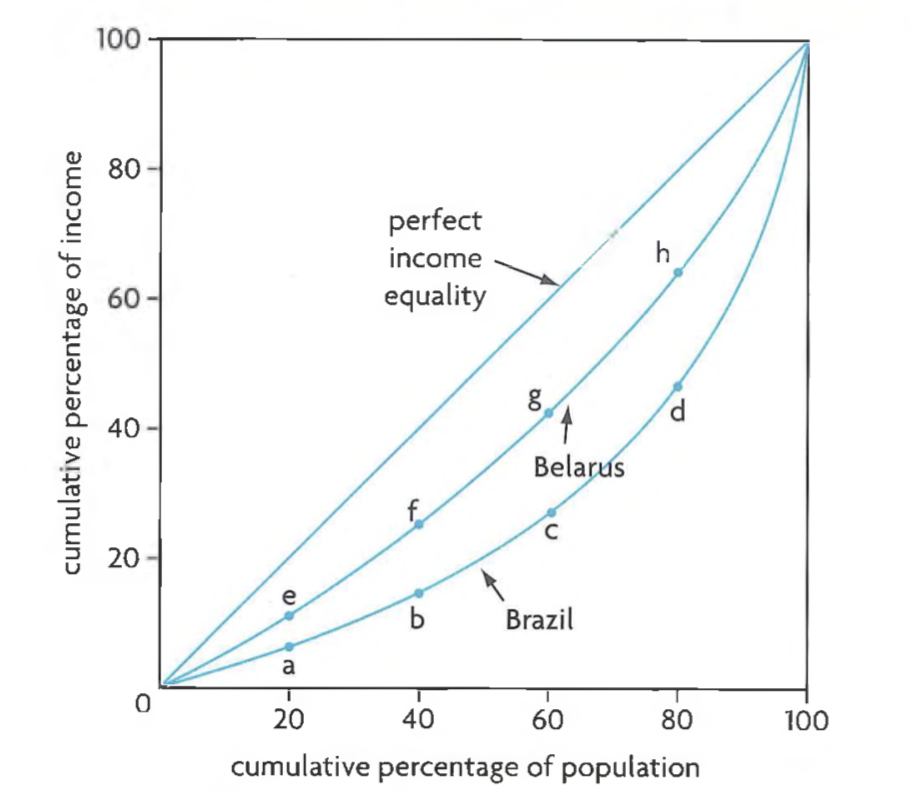
\includegraphics[width=0.5\linewidth]{Screenshot 2026-07-29 at 14.42.43.png}
\end{center}
\subsubsection*{The Gini coefficient}
$$\text{Gini coefficient}=\dfrac{\text{area between diagonal and Lorenz curve}}{\text{entire area under diagonal}}$$
\begin{itemize}
  \item Perfect income equality: 0
  \item Greatest income inequality: 1
\end{itemize}
Everything that has been said above about measurement of income inequality applies also to wealth inequality.\\
The distribution of wealth is generally far more unequal than the distribution of income in most countries in the world. On average, Gini coefficients in the case of wealth distribution are roughly double the size of the Gini coefficients of income distribution. Why?
\begin{itemize}
  \item Limited growth in wages makes it difficult for low-income and middle-income people to save and accumulate wealth.
  \item High-income people tend to consume a smaller fraction of their income than lower-income people therefore have greater possibilities of saving and accumulating wealth.
  \item Income and wealth inequalities feed on each other.
\end{itemize}
\subsection{Poverty}
\needbold{Poverty}: an inability to satisfy minimum consumption needs.
\begin{itemize}
  \item \needbold{Absolute poverty}: doesn't have enough income to meet basic human needs / income below poverty line (``minimally sufficient to sustain life'')
  \item \needbold{Relative poverty}: compares the income of individuals or households in a society with median incomes.
\end{itemize}
\subsubsection*{Measuring poverty}
\textbf{Minimum income standards (MIS)} (Joseph Rowntree Foundation, UK): ongoing research on what people believe are essentials for a minimum acceptable standard of living. Produces budgets for a basket of goods (food, clothing, housing, childcare, fuel, social/cultural participation) $\to$ calculates the minimum income required for different household types. Reveals: number of people below MIS, contribution of each item, and changes over time.
\\\\
\textbf{Multidimensional Poverty Index (MPI)}: measures poverty in three \textbf{dimensions} via ten \textbf{indicators}:
\begin{itemize}
  \item \textbf{Health}: child mortality, nutrition.
  \item \textbf{Education}: years of schooling, school attendance.
  \item \textbf{Living standards}: cooking fuel, sanitation, drinking water, electricity, housing, assets.
\end{itemize}
A person is counted as poor if deprived in at least \textbf{one-third} of the indicators. Each country receives an MPI value (0 to 1; higher = more poverty). Covers 105 countries / 5.7 billion people. Based on the concept of \textbf{deprivations} (Amartya Sen, Nobel laureate). Can be broken down by indicator to identify key contributors to poverty in each country.
\\\\
\textbf{World Bank MPI} (in development): complements UNDP/Oxford MPI by adding a \textbf{monetary indicator} (income per capita) plus additional indicators: electricity, child school enrolment, health service coverage, adult school attainment, malnourishment, water/sanitation quality, crime incidence, natural disaster incidence.

\subsubsection*{Difficulties in measuring poverty}
\begin{itemize}
  \item \textbf{Different meanings and approaches}: absolute vs.\ relative poverty, income-based vs.\ multidimensional --- these are not consistent with each other.
  \item \textbf{Measurement problems}:
  \begin{itemize}
    \item Income measures ignore \textbf{wealth and savings} that people can fall back on.
    \item Household surveys are \textbf{subjective}; exclude \textbf{homeless and institutionalised} people ($\to$ underestimates); freelance/investment income may be \textbf{understated} ($\to$ overestimates).
    \item \textbf{Urban areas} have higher costs of living $\to$ national poverty lines may exclude many urban poor.
    \item Poverty lines show \textbf{how many} fall below but not \textbf{how far below} --- depth of poverty is not captured.
  \end{itemize}
  \item \textbf{Over/underestimation of the national poverty line}: governments may \textbf{overestimate} (to receive more foreign aid) or \textbf{underestimate} (to spend less on poverty reduction programmes).
\end{itemize}
\subsection{Causes of economic inequality and poverty}
\begin{itemize}
  \item \textbf{Inequality of opportunity} (``lottery of birth''): inequalities in potential living standards arising from circumstances \textit{beyond one's control} --- parents' education/occupation/income, place of birth, gender, race/ethnicity. Studies show these contribute 4\% (Norway) to 51\% (Guatemala) of economic inequality. Distinct from \textbf{economic inequality} (inequalities in actual outcomes from income/wealth differences).
  \item \textbf{Different levels of human capital}: low education/skills/health $\to$ low productivity $\to$ low incomes; positive relationship between skill/education and income.
  \item \textbf{Different levels of resource ownership}: some inherit or accumulate financial capital/property $\to$ income and wealth advantage; others rely only on labour; renters pay rent without building wealth (unlike mortgage-paying homeowners).
  \item \textbf{Discrimination}: racial/ethnic groups and women face lower wages, greater difficulty finding work, poorer living environments, less access to services; women are at higher poverty risk (unpaid caring work, lower pay, lower pensions).
  \item \textbf{Unequal status and power}: high-status groups influence government policies to \textit{protect their own incomes/wealth} rather than favour redistribution.
  \item \textbf{Government tax and benefits policies}: reduced transfer payments/social services push low-income groups into poverty; tax policies favouring the rich increase inequality.
  \item \textbf{Technological change}: automation eliminates low-skill jobs (wages stagnate) while increasing demand for high-skill workers (wages rise) $\to$ widening skill-based wage gap; owners of capital benefit, widening labour-vs-capital income gap.
  \item \textbf{Globalisation}: FDI increases demand for skilled over unskilled workers $\to$ widening income gap; offshoring reduces domestic demand for certain skills in developed countries.
  \item \textbf{Market-based supply-side policies} (since 1980s): weakening unions, reducing minimum wage, reducing employment protection $\to$ increased inequality.
  \item \textbf{High abnormal profits of firms with market power}: monopolies/oligopolies charge higher prices $\to$ income transferred from consumers to firm owners.
  \item \textbf{Increases in executive pay}: CEO-to-average-worker pay ratio rose from 20:1 (1965) to 300:1 (2013) in the US.
  \item \textbf{Unemployment}: no income (or low benefits); long-term unemployment (structural) $\to$ high poverty risk, especially for single-parent or dual-unemployed households.
  \item \textbf{Geography}: remote/isolated regions with limited employment and relocation possibilities (rural areas in developing countries).
  \item \textbf{Age}: older people may receive inadequate or no pensions (especially in informal economies in developing countries).
  \item \textbf{Poverty itself} (\textbf{poverty cycle}): low incomes $\to$ low access to health/education/housing $\to$ low human capital $\to$ low incomes $\to$ self-perpetuating cycle.
\end{itemize}
\subsection{The impact of income and wealth inequality}
\begin{itemize}
  \item \textbf{Economic growth}: IMF studies confirm high inequality \textbf{lowers growth}. An increasing income share of the top 20\% reduces GDP growth; an increasing share of the bottom 20\% \textit{raises} growth. Reasons:
  \begin{itemize}
    \item Lower-income households cannot invest in \textbf{human and physical capital} (poor education $\to$ lower productivity $\to$ lower growth).
    \item Inequality of opportunity in education is \textbf{transferred across generations}.
    \item Wealthy spend a lower fraction of income; their savings often \textbf{leave the country} as foreign investments $\to$ less domestic investment.
    \item Concentrated wealth $\to$ \textbf{political control} by the rich $\to$ policies favouring themselves (e.g.\ deregulation leading to the 2008 financial crisis; less spending on merit goods).
    \item More equal distribution increases demand for \textbf{locally produced goods} $\to$ local production, employment, investment (especially relevant in developing countries).
    \item Poor cannot obtain \textbf{credit} (no collateral/wealth) $\to$ fewer investments in education, health, business $\to$ lower growth.
    \item Greater equality $\to$ greater \textbf{political stability}; high inequality $\to$ unrest, instability $\to$ lower growth.
  \end{itemize}
  \item \textbf{Low living standards}: greater psychological stress, substance abuse, poor nutrition/health $\to$ poorer job prospects; plus:
  \begin{itemize}
    \item \textbf{Lack of access to health care and education} $\to$ lower human capital $\to$ poverty cycle.
    \item \textbf{Higher infant, child and maternal mortality} (poor nutrition + lack of health care).
    \item \textbf{Higher preventable diseases} (poor hygiene and nutrition).
    \item \textbf{Social problems}: crime, drug use, family breakdowns, homelessness.
    \item \textbf{Inability to realise full potential} $\to$ waste of human talent $\to$ lower growth (PPC/LRAS shift less).
  \end{itemize}
  \item \textbf{Social and political stability}: inequality creates \textbf{polarised, divided societies} with reduced social solidarity and trust. Economic inequality leads to \textbf{political inequality} (rich influence policies in their favour $\to$ \textbf{vicious circle} of widening inequality). Growing dissatisfaction among lower groups may lead to \textbf{social instability and conflict}; consensus on challenges becomes harder as divisions widen.
\end{itemize}
\subsection{Policies to reduce income and wealth inequalities and poverty}
\subsubsection*{Taxation policies}
\textbf{Direct taxes} (paid directly to government by the taxpayer):
\begin{itemize}
  \item \textbf{Personal income taxes}: the most important revenue source in many countries; paid on all forms of income (wages, rent, interest, dividends).
  \item \textbf{Corporate income taxes}: taxes on profits of corporations.
  \item \textbf{Wealth taxes}: taxes on ownership of assets (property taxes, inheritance taxes).
  \item \textbf{Social insurance (social security) contributions / payroll taxes}: paid by workers and employers; revenues go into \textit{specific funds} (pensions, health care), not the general budget.
\end{itemize}
\textbf{Indirect taxes} (paid indirectly through suppliers/sellers):
\begin{itemize}
  \item \textbf{General expenditure taxes (sales taxes / VAT)}: fixed percentage of retail price (sales tax, US) or tax on value added at each production stage (VAT, EU/many countries). Some necessities (food, medicine) may be exempt/reduced on equity grounds.
  \item \textbf{Excise taxes}: on specific goods (cigarettes, petrol).
  \item \textbf{Customs duties (tariffs)}: on imports --- to make imports more expensive and/or raise revenue.
\end{itemize}
Tax systems vary enormously across countries in mix, rates and reliance on direct vs.\ indirect taxes.

\subsubsection*{Proportional, progressive and regressive taxation}
Defined by the relationship between income and the \textbf{fraction of income paid as tax}:
\begin{itemize}
  \item \textbf{Proportional}: tax rate is \textit{constant} as income rises (e.g.\ 15\% for all).
  \item \textbf{Progressive}: tax rate \textit{increases} as income rises (e.g.\ 10\% $\to$ 20\% $\to$ 30\%) $\to$ after-tax income distribution becomes \textbf{more equal}. The more progressive the system, the greater the equality achieved.
  \item \textbf{Regressive}: tax rate \textit{decreases} as income rises $\to$ after-tax distribution becomes \textbf{less equal}.
\end{itemize}
Corporate income taxes and social insurance contributions are usually \textbf{proportional}. All \textbf{indirect taxes are regressive}: a fixed tax on a good takes a \textit{larger} fraction of a low-income earner's income than a high-income earner's. 
\\\\Marginal tax rate: tax rate paid on additional income.\\
Average tax rate: tax paid divided by total income.\\
Tax brackets: different layers of income, used in progressive tax system. The corresponding tax rates are the marginal tax rates.
\[\text{Indirect tax}=\dfrac{r}{100}\times \dfrac{S}{1+\dfrac{r}{100}}\]
where $S$ is the amount available for purchases and $r$ is the rate of indirect tax.

\subsubsection*{Achieving progressivity through proportional taxation (supplementary)}
Some countries (e.g.\ Estonia, Latvia, Lithuania) use \textbf{flat (proportional) personal income taxes}, yet these systems are still \textbf{progressive in practice} because they contain \needbold{exclusions}: an amount of income that is not taxed at all. Example with a \pounds10\,000 exclusion and a 15\% flat rate on taxable income:
\begin{center}
\begin{tabular}{cccc}
\toprule
\textbf{Income (\pounds)} & \textbf{Taxable income (\pounds)} & \textbf{Tax (\pounds)} & \textbf{Effective tax rate} \\
\midrule
10\,000 & 0 & 0 & 0\% \\
15\,000 & 5\,000 & 750 & 5\% \\
20\,000 & 10\,000 & 1\,500 & 7.5\% \\
25\,000 & 15\,000 & 2\,250 & 9\% \\
\bottomrule
\end{tabular}
\end{center}
Because the \textbf{effective tax rate rises} with income, the proportional tax has become progressive. Since virtually all flat-tax systems include exclusions, almost all personal income tax systems worldwide are progressive in effect (differing in degree). A similar effect can be created with tax \textbf{credits} or \textbf{allowances}.

\subsubsection*{Evaluating taxes as a redistribution policy}
\begin{itemize}
  \item In advanced economies, $\sim$25\% of redistribution occurs through taxes (75\% through benefits/transfer payments).
  \item \textbf{Case for progressive taxes}: strong evidence that high inequality harms growth $\to$ progressive taxes (income, corporate, wealth) would \textit{reduce inequality and support growth}. Less reliance on regressive indirect taxes.
  \item \textbf{Case against (disincentive effects)}: progressive income taxes reduce after-tax income $\to$ \textbf{disincentive to work and save}, especially for high earners; corporate taxes reduce incentives to invest; wealth taxes may reduce efficiency/innovation $\to$ lower growth. This thinking aligns with market-based supply-side policies.
\end{itemize}
\subsubsection*{Other redistribution policies}
\textbf{Investment in human capital} (reducing inequality of opportunity):
\begin{itemize}
  \item Disadvantaged groups have far lower educational attainment and health care access
  \item Government must ensure \textbf{universal access} to quality education and health care, provided \textbf{free of charge} (not relying on out-of-pocket/private payments beyond the reach of the poor).
\end{itemize}
\textbf{Transfer payments (cash transfers)}: government payments to \textbf{vulnerable groups}. Include old-age pensions, unemployment benefits, child allowances, housing benefits, disability pensions, etc. Financed by taxes; contribute $\sim$75\% of redistribution in developed countries. \textit{Disadvantages}: budget burden, opportunity costs; debated disincentive to work.
\\
\textbf{Targeted government spending on goods and services}:
\begin{itemize}
  \item Provision of \textbf{merit goods} (education, health care, infrastructure: clean water, sanitation) free or at very low prices, financed by tax revenue.
  \item Also corrects positive consumption externalities (market failure).
  \item \textit{Disadvantage}: budget burden and opportunity costs.
\end{itemize}
\textbf{Universal basic income (UBI)}: a fixed sum paid to \textit{all} residents regardless of other income. Purpose: reduce inequality/poverty; gaining popularity due to rising inequality and automation fears.
\begin{itemize}
  \item \textit{Pros}: administratively simple; supports students, unpaid carers, entrepreneurs; stabilises economy in recession (automatic stabiliser); gives workers more bargaining power.
  \item \textit{Cons}: very expensive (goes to all including those who don't need it); may require cutting other social services; possible work disincentive; opportunity costs.
\end{itemize}
\textbf{Policies to reduce discrimination}: anti-discrimination legislation; education of employers/workers on multiculturalism benefits; management training; communication of anti-discrimination policies. \textit{Limitation}: employers may not always comply.
\\
\textbf{Government intervention in markets (price controls)}:
\begin{itemize}
  \item \textbf{Minimum wage legislation}: raises wages of low-income/unskilled workers above equilibrium. Standard theory predicts unemployment, but practice shows this is most often \textit{not} the case $\to$ improves income distribution.
  \item \textbf{Food price ceilings}: make food more affordable for low-income groups; \textbf{rent controls}: support low-income tenants.
  \item \textbf{Price floors for farmers}: raise farmers' incomes (often with government purchases of surpluses).
  \item \textit{Disadvantage}: all price controls lead to \textbf{allocative inefficiency} and loss of social surplus.
\end{itemize}
\section{Demand-side and supply-side policies}
\subsection{Introduction to macroeconomic policies}
Demand-side policies: focus on changing / shifting AD to achieve macroeconomic aims. Counteract the effects of short-term fluctuations that cause inflationary / recessionary gaps and bring AD to potential GDP. Including monetary policies and fiscal policies. Also called stabilization policies.\\
Supply-side policies: focus on the production of the economy, shifting LRAS / Keynesian AS \textbf{to the right} to increase potential output and achieve long-term economic growth. Focus on improving the quality and quantity of FoPs and institutional changes to improve productive capacity. Including market-based and interventionist approach.
\subsection{Demand management and monetary policy}
\textbf{Central bank vs.\ commercial banks}: commercial banks hold deposits, make loans, transfer funds, and buy government bonds for customers. The \textbf{central bank} is a government institution with four main responsibilities:
\begin{itemize}
  \item \textbf{Banker to the government}: holds government deposits, receives/makes payments, manages borrowing by selling bonds.
  \item \textbf{Banker to commercial banks}: holds their deposits and makes loans to them in times of need (not a banker to consumers/firms).
  \item \textbf{Regulator of commercial banks}: supervises to ensure appropriate cash levels and financial system safety.
  \item \textbf{Conducts monetary policy}: controls money supply and interest rates.
\end{itemize}
\textbf{Central bank independence}: in many countries the central bank has a degree of independence from political interference, ensuring monetary policy serves the longer-term interests of the economy (e.g.\ not stimulating artificially before elections). Global trend toward greater independence.

\subsubsection*{Goals of monetary policy}
\begin{itemize}
  \item \textbf{Low and stable rate of inflation} (often $\sim$2\% --- low but not dangerously close to deflation).
  \item \textbf{Low unemployment} (particularly cyclical unemployment from insufficient AD).
  \item \textbf{Reduce business cycle fluctuations}: minimise disruptive inflation (above potential output) and cyclical unemployment (below potential).
  \item \textbf{Promote a stable economic environment for long-term growth}: firms need stability to plan investment, R\&D and innovation.
  \item \textbf{External balance}: export revenues balanced by import spending over time; the central bank influences exchange rates through the interest rate--exchange rate relationship.
\end{itemize}

\subsubsection*{Inflation targeting}
An increasing number of central banks target a specific inflation rate (typically 1.5--2.5\%, with $\pm$1\% tolerance margin), based on CPI forecasts.\\
\textbf{Advantages}:
\begin{itemize}
  \item Achieves a low and stable rate of inflation.
  \item Improves ability of firms/consumers to \textbf{anticipate future inflation} and plan accordingly.
  \item Enables greater \textbf{co-ordination between monetary and fiscal policy}.
\end{itemize}
\textbf{Disadvantages}:
\begin{itemize}
  \item \textbf{Reduced ability to pursue other objectives}, especially full employment (given the inflation--unemployment conflict).
  \item \textbf{Reduced ability to respond to supply-side shocks}: e.g.\ oil price spikes causing cost-push inflation/stagflation may require expansionary policy with above-target inflation.
  \item A target that is \textbf{too low} may cause higher unemployment; \textbf{too high} may lead to problems of high inflation.
\end{itemize}
Monetary policy impacts indirectly on aggregate demand through the interest rate. The interest rate is affected by level of risk of loan, maturity (time to pay back the loan), size of loan, degree of market power.\\\\
Money: anything that is acceptable as payment for goods and services, including currency, cheque accounts.

\subsubsection*{Supplementary: Functions and measures of money (AP Barron Ch 14)}
\begin{itemize}
  \item \textbf{Three primary functions of money}:
  \begin{itemize}
    \item \textbf{Medium of exchange}: facilitates transactions and eliminates the need for the double coincidence of wants required under barter.
    \item \textbf{Unit of account}: provides a common measure and standard for quoting prices, calculating profits, and keeping economic records.
    \item \textbf{Store of value}: allows purchasing power to be transferred from the present to the future (subject to inflation risk).
    \item (\textit{Standard of deferred payment}: serves as a measure for settling debts contracted in the present to be repaid in the future.)
  \end{itemize}
  \item \textbf{Monetary aggregates}:
  \begin{itemize}
    \item \needbold{Narrow money (M1)}: highly liquid money used directly for transactions, consisting of physical currency in circulation plus demand (checking) deposits.
    \item \needbold{Broad money (M2)}: M1 plus savings deposits, small-denomination time deposits, and money market deposit accounts (near-money).
    \item \needbold{Monetary base (M0)}: total currency in circulation plus commercial bank reserve balances held at the central bank.
  \end{itemize}
  \item \needbold{Fiat money}: currency that has no intrinsic commodity value (not backed by gold or silver) and derives its value solely from government decree (legal tender) and public acceptance.
\end{itemize}

The rate of interest can be thought of as the 'price' of money services. The supply of money is fixed at a level decided upon by the central bank.\\
The demand for money has the familiar downward-sloping shape of a demand curve. \\
An increase in the supply of money leads to a fall in the rate of interest; a decrease in the supply of money leads to an increase in the rate of interest.
\begin{center}
  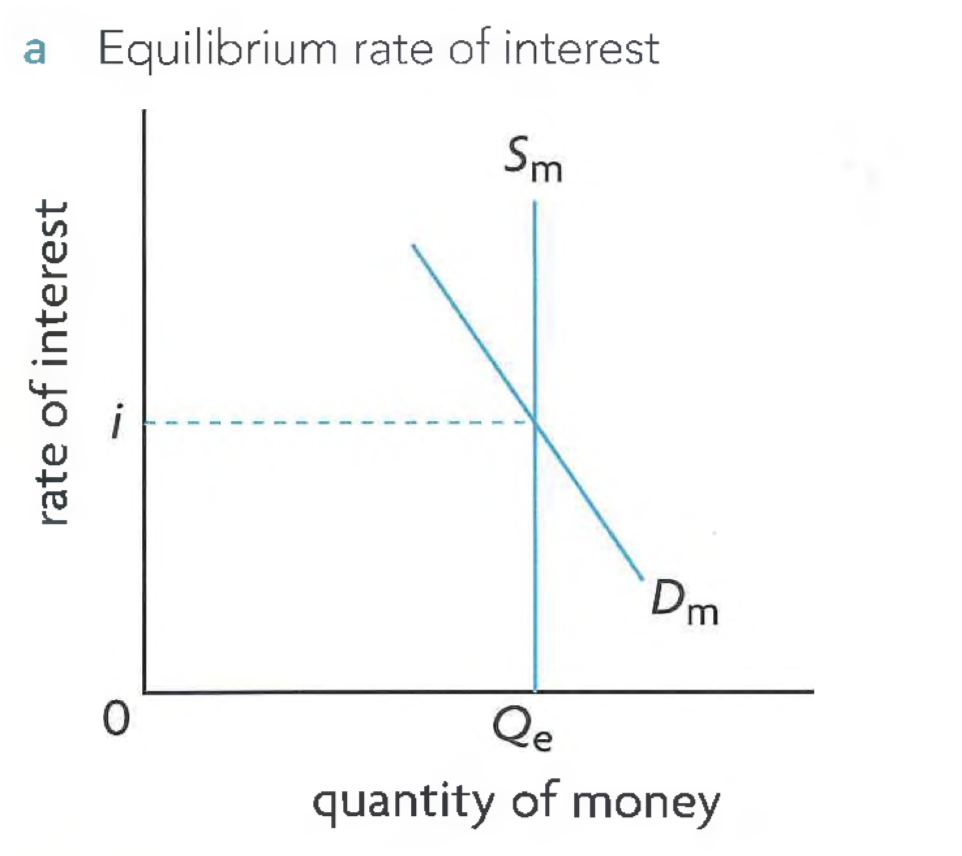
\includegraphics[width=0.32\linewidth]{Screenshot 2026-07-29 at 19.51.43.png}
  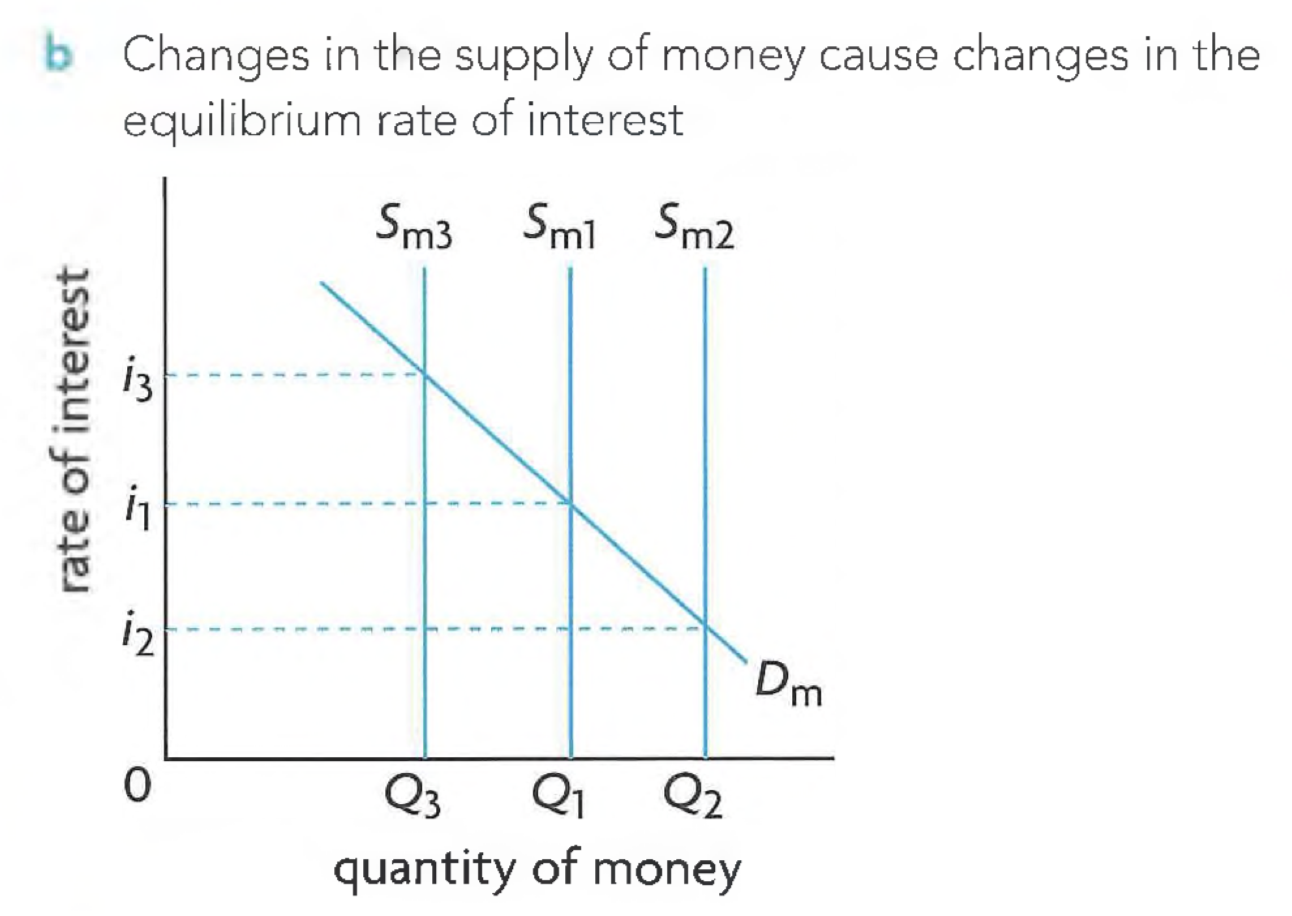
\includegraphics[width=0.4\linewidth]{Screenshot 2026-07-29 at 19.51.54.png}
\end{center}
\subsubsection*{How the central bank changes the money supply}
Commercial banks lend savers' deposits to borrowers. (In a fractional reserve system) The funds they must legally keep are called required reserves, which are a legally determined fraction of total deposits, called the minimum reserve requirement or required reserve ratio. The rest are called excess reserves and can be lent out. Over time the amount of loans will continue to get larger and larger. The initial excess reserves and amount of new loans created is correlated via the "monetary multipler" = $\dfrac{1}{\text{RRR}}$. These new loans are the money created.\\\\
Tools of monetary policies:
\begin{itemize}
  \item Open market operations: buying (increase MS) and selling bonds (decrease MS)
  \item Minimum reserve requirement: higher the RRR, lower the MS
  \item Minimum lending rate / discount rate: interest rate for central banks lend money to commercial banks. Lower the discount rate, higher the MS.
  \item Quantitative easing 量化宽松: Similar to OMO but on a larger scale (huge amount of assets that the commercial banks own). 
\end{itemize}

\subsubsection*{Supplementary: The reserve market (federal funds market) (AP)}
The \needbold{reserve market} (in the US, the \needbold{federal funds market}) is the operational interbank market where commercial banks borrow and lend reserve balances to each other on an overnight basis. The equilibrium interest rate determined in this market is the \needbold{federal funds rate} --- the principal operating target of central bank monetary policy.
\begin{itemize}
  \item \textbf{Demand for reserves ($D_r$)}: downward-sloping. Banks demand reserves to meet legal reserve requirements and to manage clearing and liquidity risks. As the federal funds rate rises, the opportunity cost of holding excess reserves increases, so the quantity of reserves demanded falls.
  \item \textbf{Supply of reserves ($S_r$)}: vertical. The central bank has monopoly control over the total volume of reserves created in the banking system, primarily through \textbf{open market operations}.
  \item \textbf{Monetary policy implementation}:
  \begin{itemize}
    \item \textbf{Expansionary policy}: the central bank \textbf{buys government securities} from banks $\to$ pays by crediting bank reserve accounts $\to S_r$ shifts \textbf{right} $\to$ the federal funds rate \textbf{falls} ($r_1 \to r_2$). Commercial banks experience lower borrowing costs and expand lending to households and businesses, lowering broader market interest rates and shifting AD rightward.
    \item \textbf{Contractionary policy}: the central bank \textbf{sells government securities} $\to$ deducts reserves from buyer banks' accounts $\to S_r$ shifts \textbf{left} $\to$ the federal funds rate \textbf{rises}, raising commercial borrowing rates and shifting AD leftward.
    \item \textbf{Administered rates}: the \textbf{discount rate} (lending rate directly from the central bank) acts as an upper ceiling for the market rate, while interest paid on reserve balances (IORB) sets a lower floor.
  \end{itemize}
\end{itemize}
\begin{center}
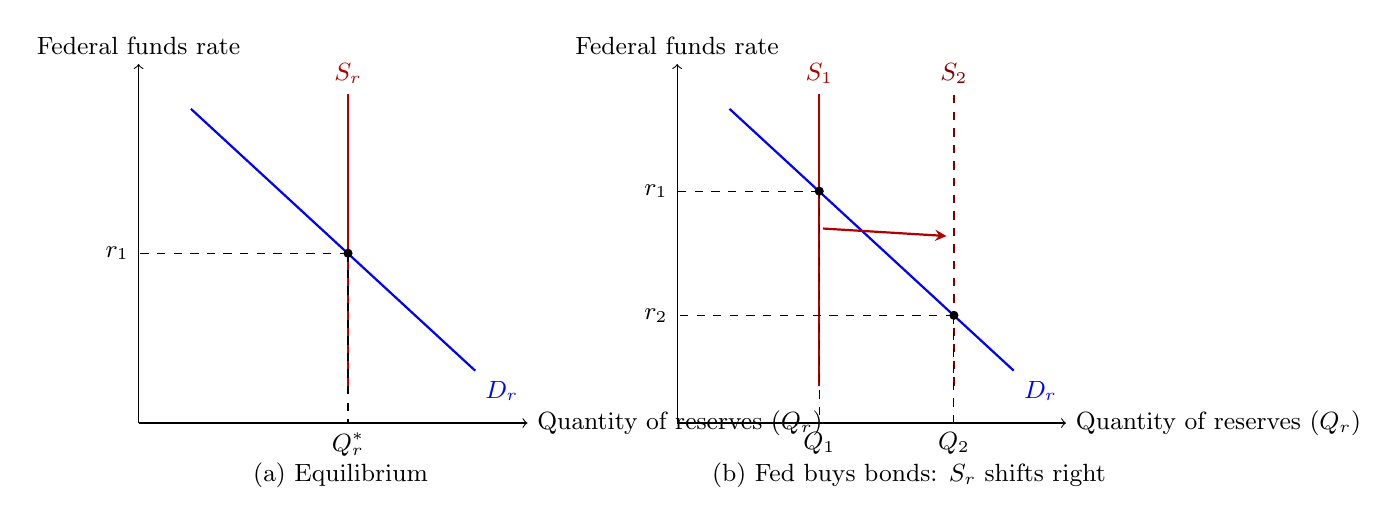
\begin{tikzpicture}[scale=0.95]
% --- Panel (a): equilibrium ---
\begin{scope}
\draw[->] (0,0) -- (5.2,0) node[right, font=\small] {Quantity of reserves ($Q_r$)};
\draw[->] (0,0) -- (0,4.8) node[above, font=\small] {Federal funds rate};
\draw[thick, blue] (0.7,4.2) -- (4.5,0.7) node[below right, blue, font=\small] {$D_r$};
\draw[thick, red!70!black] (2.8,0.5) -- (2.8,4.4) node[above, red!70!black, font=\small] {$S_r$};
\filldraw (2.8,2.27) circle (1.5pt);
\draw[dashed] (2.8,2.27) -- (2.8,0) node[below, font=\small] {$Q_r^*$};
\draw[dashed] (2.8,2.27) -- (0,2.27) node[left, font=\small] {$r_1$};
\node[font=\small] at (2.7,-0.7) {(a) Equilibrium};
\end{scope}
% --- Panel (b): expansionary open market operation ---
\begin{scope}[xshift=7.2cm]
\draw[->] (0,0) -- (5.2,0) node[right, font=\small] {Quantity of reserves ($Q_r$)};
\draw[->] (0,0) -- (0,4.8) node[above, font=\small] {Federal funds rate};
\draw[thick, blue] (0.7,4.2) -- (4.5,0.7) node[below right, blue, font=\small] {$D_r$};
\draw[thick, red!70!black] (1.9,0.5) -- (1.9,4.4) node[above, red!70!black, font=\small] {$S_1$};
\draw[thick, red!50!black, dashed] (3.7,0.5) -- (3.7,4.4) node[above, red!50!black, font=\small] {$S_2$};
\filldraw (1.9,3.1) circle (1.5pt);
\filldraw (3.7,1.44) circle (1.5pt);
\draw[dashed] (1.9,3.1) -- (0,3.1) node[left, font=\small] {$r_1$};
\draw[dashed] (3.7,1.44) -- (0,1.44) node[left, font=\small] {$r_2$};
\draw[dashed] (1.9,3.1) -- (1.9,0) node[below, font=\small] {$Q_1$};
\draw[dashed] (3.7,1.44) -- (3.7,0) node[below, font=\small] {$Q_2$};
\draw[->, >=stealth, thick, red!70!black] (1.95,2.6) -- (3.6,2.5);
\node[font=\small] at (3.1,-0.7) {(b) Fed buys bonds: $S_r$ shifts right};
\end{scope}
\end{tikzpicture}
\end{center}

Nominal IR: the market rate that prevails at any moment in time.\\
Real IR: the interest rate that has been corrected for inflation, = Nominal IR - Rate of inflation.

\subsubsection*{Supplementary: Quantity theory of money, loanable funds and the Fisher effect (AP Barron Ch 15)}
\begin{itemize}
  \item \needbold{Equation of exchange / quantity theory of money}:
  \[MV = PY\]
  where $M$ = money supply, $V$ = velocity of money (how many times a unit of currency changes hands), $P$ = price level, and $Y$ = real GDP ($PY$ = nominal GDP).
  \begin{itemize}
    \item Classical and monetarist assumption: $V$ and real output $Y$ are determined by real factors and are relatively stable in the long run.
    \item Therefore, any increase in money supply ($M$) translates proportionally into a higher price level ($P$) --- ``inflation is always and everywhere a monetary phenomenon''.
  \end{itemize}
  \item \needbold{Loanable funds market}: a model analysing the real interest rate determined by the demand for and supply of loanable funds:
  \begin{itemize}
    \item \textbf{Demand for loanable funds}: originates from firms undertaking \textbf{investment} expenditure and government borrowing to finance deficits (downward-sloping with respect to the real interest rate).
    \item \textbf{Supply of loanable funds}: originates from household and business \textbf{savings} plus foreign capital inflows (upward-sloping with respect to the real interest rate).
    \item \textbf{Crowding out}: government budget deficits increase the demand for loanable funds (shifting demand right), which pushes up the real interest rate and crowds out private investment.
  \end{itemize}
  \item \needbold{Fisher effect}: the nominal interest rate equals the real interest rate plus the expected inflation rate:
  \[\text{Nominal interest rate} \approx \text{Real interest rate} + \text{Expected inflation}\]
  In the long run, changes in expected inflation lead to one-for-one adjustments in nominal interest rates, leaving the equilibrium real interest rate determined by savings and investment fundamentals.
\end{itemize}

Two types of MS:
\begin{itemize}
  \item \textbf{Expansionary (easy money) policy}: used in a \textbf{deflationary/recessionary gap}. Central bank \textbf{increases money supply} $\to$ interest rate \textbf{falls} $\to$ lower cost of borrowing $\to$ consumers and firms borrow/spend more ($C \uparrow$, $I \uparrow$) $\to$ AD shifts \textbf{right} $\to$ real GDP rises toward potential output, closing the recessionary gap.
  \begin{itemize}
    \item Monetarist/new classical: AD increase raises both real GDP \textbf{and} the price level (upward-sloping SRAS).
    \item Keynesian: if AD shifts within the \textbf{horizontal} part of the AS curve, real GDP rises with \textbf{no} price-level increase; only a small price rise if AD reaches the upward-sloping part.
  \end{itemize}
  \item \textbf{Contractionary (tight money) policy}: used in an \textbf{inflationary gap}. Central bank \textbf{decreases money supply} $\to$ interest rate \textbf{rises} $\to$ higher cost of borrowing $\to$ consumers and firms borrow/spend less ($C \downarrow$, $I \downarrow$) $\to$ AD shifts \textbf{left} $\to$ real GDP falls back to potential output, closing the inflationary gap and reducing inflation.
  \begin{itemize}
    \item Monetarist/new classical: AD decrease lowers both real GDP \textbf{and} the price level.
    \item Keynesian: if AD falls within the upward-sloping part, effects are similar to the monetarist model. But if AD falls into the \textbf{horizontal} part, real GDP falls more and the price level falls less (or not at all).
  \end{itemize}
\end{itemize}
\textbf{The ratchet effect (Keynesian)}: the price level rises easily with strong AD but \textbf{does not easily fall} when AD decreases. In practice, a decrease in AD lowers real GDP while the price level \textbf{remains constant} --- a more realistic representation. This means a \textit{smaller} decrease in AD is needed to return to potential output compared with the model without the ratchet effect.

\subsubsection*{Evaluation of monetary policy}
\textbf{Constraints (weaknesses):}
\begin{itemize}
  \item \textbf{Possible ineffectiveness in deep recession}: (i) interest rates cannot fall below \textbf{zero}; (ii) low consumer/producer confidence $\to$ firms and consumers avoid borrowing even at low rates; (iii) banks may be \textbf{fearful of lending} (borrowers may default). Occurred in the Great Depression (1930s), Japan (late 1990s--2000s), and the global recession (2008).
  \item \textbf{Conflict between government objectives}: interest rate changes affect both domestic variables ($C$, $I$, inflation, unemployment) and the foreign sector (exchange rates) $\to$ pursuing domestic goals may conflict with external balance.
  \item \textbf{May be inflationary}: if expansionary policy lasts too long, AD may increase beyond what is needed to close the recessionary gap.
  \item \textbf{Ineffective against stagflation / cost-push inflation}: monetary policy is a \textit{demand-side} tool and cannot address supply-side causes of instability.
\end{itemize}
\textbf{Strengths:}
\begin{itemize}
  \item \textbf{Incremental}: interest rates can be adjusted in very small steps $\to$ well suited to ``fine-tuning''.
  \item \textbf{Reversible}: expansionary can easily become contractionary and vice versa.
  \item \textbf{Flexible}: interest rates can be changed frequently as needed.
  \item \textbf{Relatively short time lags}: can be implemented quickly (though effects take time; lags are shorter than fiscal policy).
  \item \textbf{Central bank independence}: can pursue policies in the longer-term interests of the economy, even if politically unpopular (e.g.\ raising interest rates).
  \item \textbf{Limited political constraints}: does not involve changes to government spending or taxes (unlike fiscal policy).
  \item \textbf{No budget deficits or debt}: does not increase government debt (unlike expansionary fiscal policy).
  \item \textbf{No crowding out}: does not lead to crowding out (a potential weakness of fiscal policy; see below).
\end{itemize}
\subsection{Demand management and fiscal policy}
\needbold{Fiscal policy} refers to manipulations by the government of its own expenditures and taxes to influence the level of aggregate demand.\\\\
The \needbold{government budget}: a type of plan of a country's revenues and expenditures over a period of time that the government makes to plan its activities.\\\\
Sources of government revenue:
\begin{itemize}
  \item Taxes of all types.
  \item From the sales of G\&S.
  \item From the sale of government-owned (state-owned) assets, or property.
\end{itemize}
Types of government expenditure:
\begin{itemize}
  \item Current expenditure: government's spending on day-to-day items that are recurring and items that are used up or 'consumed' as a G\&S is provided. 
  \item Capital expenditure: public investments, or spending to produce physical capital.
  \item Transfer payments:  payments by the government to vulnerable groups for the purposes of income redistribution. (Not included in government spending)
\end{itemize}
The goals of fiscal policies:
\begin{itemize}
  \item \textbf{Low and stable rate of inflation}: manipulate taxes and government spending to influence AD. No inflation target (unlike monetary policy), but may complement monetary policy.
  \item \textbf{Low unemployment}: influence AD to reduce \textbf{cyclical} unemployment in deflationary gaps.
  \item \textbf{Reduce business cycle fluctuations}: minimise inflationary and deflationary gaps.
  \item \textbf{Promote a stable economic environment for long-term growth}: firms need stability (no sharp gaps) for confident investment, R\&D and innovation planning.
  \item \textbf{External balance}: influence import levels through AD effects (see Chapter 17, HL).
  \item \textbf{Equitable distribution of income}: \textit{unique to fiscal policy} (not shared with monetary policy) --- achieved through tax policies and government spending on merit goods/transfer payments.
\end{itemize}
Fiscal policy can affect three of these components: C, I, and G component of GDP.
\begin{itemize}
  \item \textbf{Expansionary fiscal policy} (used in a \textbf{recessionary gap}):
  \begin{itemize}
    \item \textbf{Increase government spending} ($G \uparrow$) $\to$ AD shifts right \textit{directly}.
    \item \textbf{Decrease personal income taxes} $\to$ disposable income rises $\to$ consumption spending increases ($C \uparrow$) $\to$ AD shifts right.
    \item \textbf{Decrease business taxes} $\to$ after-tax profits rise $\to$ investment spending increases ($I \uparrow$) $\to$ AD shifts right.
    \item \textbf{Combination} of the above. Increasing $G$ while cutting taxes is financed by \textbf{borrowing} $\to$ creates/enlarges a \textbf{budget deficit} (or shrinks a surplus).
    \item Monetarist/new classical: smaller increase in real GDP + larger price-level rise (upward-sloping SRAS). Keynesian: larger real GDP increase + smaller/no price-level rise (horizontal AS portion).
  \end{itemize}
  \item \textbf{Contractionary fiscal policy} (used in an \textbf{inflationary gap}):
  \begin{itemize}
    \item \textbf{Decrease government spending} ($G \downarrow$) $\to$ AD shifts left \textit{directly}.
    \item \textbf{Increase personal income taxes} $\to$ disposable income falls $\to$ consumption spending falls ($C \downarrow$) $\to$ AD shifts left.
    \item \textbf{Increase business taxes} $\to$ after-tax profits fall $\to$ investment spending falls ($I \downarrow$) $\to$ AD shifts left.
    \item \textbf{Combination} of the above $\to$ creates/enlarges a \textbf{budget surplus} (or shrinks a deficit).
    \item \textbf{Ratchet effect} (Keynesian): price level does not easily fall when AD decreases $\to$ real GDP falls while price level remains constant.
  \end{itemize}
\end{itemize}

\subsubsection*{Evaluation of fiscal policy}
\textbf{Constraints (weaknesses):}
\begin{itemize}
  \item \textbf{Time lags}: delays in (i) recognising the problem, (ii) deciding on policy, and (iii) the policy taking effect. By the time it works, conditions may have changed.
  \item \textbf{Political constraints}: spending cuts on merit/public goods are politically difficult; tax increases are unpopular; tax cuts may be enacted for popularity rather than necessity.
  \item \textbf{Sustainable debt}: persistent deficits from borrowing accumulate debt. In recessions, falling tax revenues + rising spending worsen deficits $\to$ risk of \textbf{unsustainable debt} or \textbf{default}.
  \item \textbf{Tax cuts less effective in recession}: part of increased after-tax income is \textbf{saved} rather than spent (especially with pessimism) $\to$ weaker AD impact. Government spending increases are more powerful (they affect AD in their entirety).
  \item \textbf{Inability to ``fine-tune''}: can move AD in a general direction but cannot precisely target output, employment, or price level.
  \item \textbf{May be inflationary}: if expansionary policy overshoots, AD rises beyond what is needed to close the gap.
  \item \textbf{Ineffective against stagflation / cost-push inflation}: fiscal policy is demand-side, cannot address supply-side causes.
  \item \textbf{Crowding out}: Government borrowing involves an increase in the demand for money, which leads to an increase in the rate of interest, leading to lower investment and consumption. Keynesian economists mainly believe that crowding out is less likely to happen, while new classical / monetarist economists hold a different opinion.
  \begin{center}
    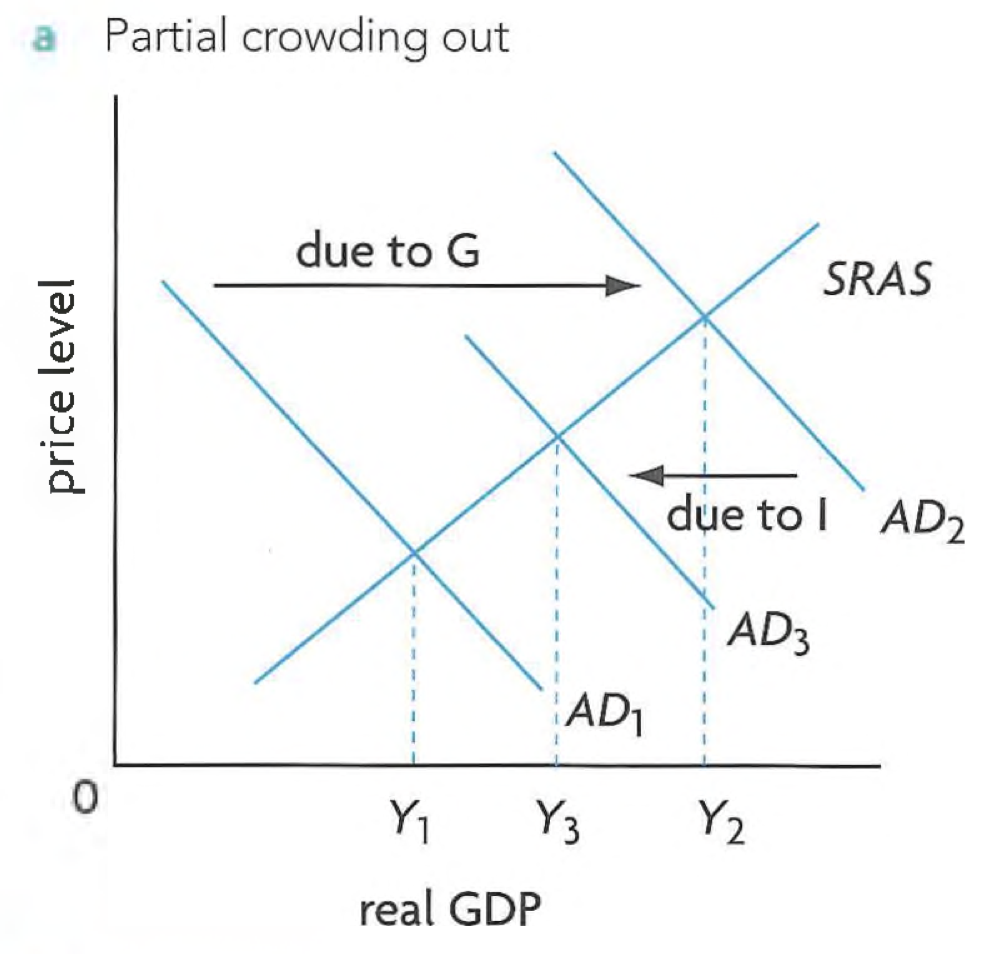
\includegraphics[width=0.35\linewidth]{Screenshot 2026-07-31 at 14.58.34.png}
    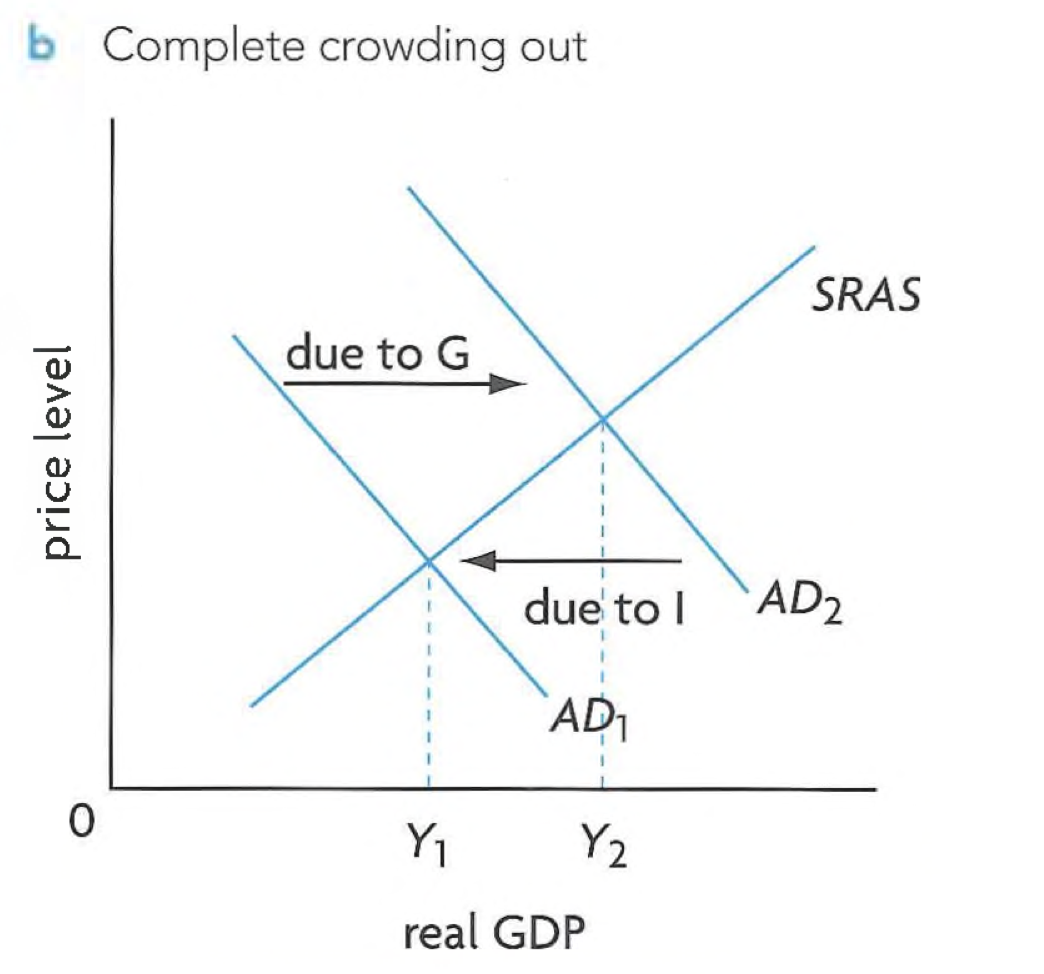
\includegraphics[width=0.35\linewidth]{Screenshot 2026-07-31 at 14.58.44.png}
  \end{center}
\end{itemize}
\textbf{Strengths:}
\begin{itemize}
  \item \textbf{Pulling an economy out of deep recession}: Keynes argued wages/prices are inflexible downward $\to$ the economy can be stuck in recession indefinitely; fiscal policy can stimulate AD directly (used globally in the 2008 recession).
  \item \textbf{Ability to target specific sectors}: education, health care, infrastructure, depressed regions, public goods --- spending can be directed by priority.
  \item \textbf{Direct impact of government spending on AD}: changes in $G$ affect AD directly (more certain than tax changes, which work indirectly via disposable income/profits).
  \item \textbf{Dealing with rapid inflation}: contractionary fiscal policy can effectively bring overheating under control.
  \item \textbf{Ability to affect potential output}: indirectly (stable macro environment) and directly (investment in human/physical capital, infrastructure, firm incentives).
\end{itemize}
\subsubsection*{Discretionary fiscal policy vs automatic stabilisers}
Fiscal policy can be classified by \textbf{how} it responds to the business cycle:
\begin{itemize}
  \item \needbold{Discretionary fiscal policy} (Edexcel definition): the \textbf{deliberate manipulation of government spending and taxes} by policy-makers to influence the economy. It requires an explicit policy decision --- a new act of government --- and includes:
  \begin{itemize}
    \item \textbf{Expansionary discretionary policy}: deliberate increases in government spending (e.g.\ a new infrastructure programme) or tax cuts (e.g.\ a legislated income-tax cut), chosen to close a recessionary gap.
    \item \textbf{Contractionary discretionary policy}: deliberate spending cuts or tax increases, chosen to close an inflationary gap.
  \end{itemize}
  \item \needbold{Automatic (built-in) stabilisers} are \textbf{already-existing rules} --- mainly progressive income taxes and welfare/unemployment benefits --- that change government spending and tax revenue \textbf{automatically} as GDP changes, \textbf{without any new decision} by policy-makers:
  \begin{itemize}
    \item in a recession, tax revenues fall automatically and welfare spending rises automatically $\to$ AD falls less than it otherwise would;
    \item in a boom, tax revenues rise automatically and welfare spending falls automatically $\to$ AD grows less rapidly (anti-inflationary).
  \end{itemize}
  \item \textbf{Key contrasts}:
  \begin{itemize}
    \item \textbf{Speed}: automatic stabilisers act immediately (no recognition/decision/implementation lag); discretionary policy suffers \textbf{time lags} --- recognition lag, decision lag and implementation/effect lag --- and may act pro-cyclically if it takes effect after the economy has already turned.
    \item \textbf{Political process}: discretionary policy requires legislation (Congress/parliament), so it is slow and politically contentious; automatic stabilisers need no vote.
    \item \textbf{Precision}: discretionary policy can target specific sectors and can be large enough to close deep gaps; automatic stabilisers only \textit{dampen} fluctuations --- they cannot prevent a recession or eliminate a gap on their own.
  \end{itemize}
  \item \textbf{Cyclical vs structural budget balances} (Edexcel):
  \begin{itemize}
    \item \textbf{Cyclical deficit/surplus}: the part of the actual fiscal balance caused by the automatic response of taxes and spending to the trade cycle. In a boom, the cyclical balance is positive (taxes high, welfare spending low); in a recession, it is negative (taxes low, welfare spending high).
    \item \textbf{Structural (cyclically adjusted) deficit/surplus}: the fiscal balance that would exist \textbf{at the peak of a boom} --- i.e.\ the actual balance with the effects of automatic stabilisers removed. A structural deficit means the government borrows even in good times, so the national debt grows over time; economists argue structural deficits need to be eliminated.
  \end{itemize}
  \item \textbf{Counter-cyclical vs pro-cyclical policy}: discretionary fiscal policy is \textbf{counter-cyclical} when the government deliberately expands in recessions and contracts in booms. Research (Edexcel) shows many \textbf{developing countries} historically behaved \textbf{pro-cyclically} (cutting spending and raising taxes in downturns --- often forced by inability to borrow --- and expanding in booms), partly because they lack significant automatic stabilisers (welfare payments are a small share of government spending). Counter-cyclical fiscal policy is easier in developed countries with credible borrowing capacity and larger automatic stabilisers.
\end{itemize}
\subsubsection*{Built-in (automatic) stabilisers}
\needbold{Built-in (automatic) stabilisers} are government policies \textbf{already in place} that automatically promote the \textbf{correct fiscal stance over the business cycle}: deficit spending (or smaller surpluses) during recessions, and surplus budgets (or smaller deficits) during expansions --- all \textbf{without any new decision by policy-makers}.
\begin{itemize}
  \item \textbf{Mechanism --- progressive income taxes}:
  \begin{itemize}
    \item In a \textbf{recession}, incomes fall $\to$ households move into lower tax brackets (or below the tax threshold) $\to$ tax revenues fall \textit{automatically} $\to$ disposable income falls by less than pre-tax income $\to$ consumption falls by less than it otherwise would. Falling tax revenues act like an automatic expansionary policy.
    \item In a \textbf{boom}, incomes rise $\to$ households move into higher tax brackets $\to$ tax revenues rise faster than incomes $\to$ disposable income and consumption grow more slowly $\to$ automatic contractionary (anti-inflationary) policy. The more progressive the tax system, the stronger this stabilising effect.
  \end{itemize}
  \item \textbf{Mechanism --- unemployment/welfare benefits} (e.g.\ unemployment insurance, anti-poverty transfer programmes such as TANF in the US):
  \begin{itemize}
    \item In a \textbf{recession}, unemployment rises $\to$ benefit payments automatically increase $\to$ the unemployed's lost income is partly replaced $\to$ consumption and AD fall less than they otherwise would.
    \item In a \textbf{boom}, unemployment falls $\to$ fewer households qualify $\to$ benefit spending automatically declines $\to$ AD grows less rapidly.
  \end{itemize}
  \item \textbf{What they can and cannot do}:
  \begin{itemize}
    \item They \textbf{dampen} fluctuations: they can prevent a recession from becoming a depression and help prevent an expansion from turning into hyperinflation.
    \item They \textbf{cannot prevent a recession or close an output gap on their own} --- a drop in income is what activates them, and they only reduce the size of the swing.
    \item They work through the \textbf{multiplier}: by reducing the size of the \textbf{MPC} (higher taxes and benefits leak more of each income change out of the spending stream), they lower the multiplier, so any given shock to AD produces smaller induced changes in real GDP (e.g.\ if unemployment benefits lower the MPC from $3/4$ to $1/2$, the multiplier falls from 4 to 2).
  \end{itemize}
\end{itemize}
\begin{center}
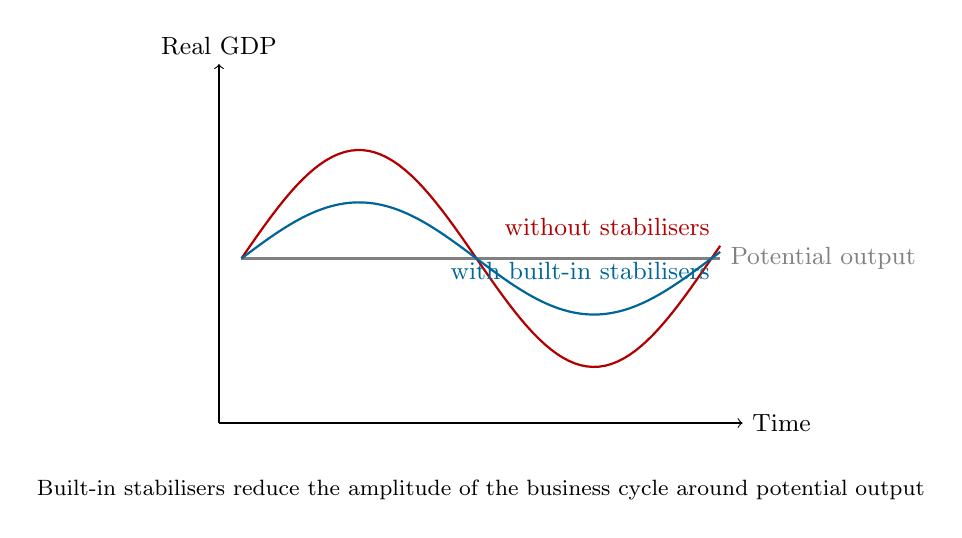
\begin{tikzpicture}[scale=0.95]
\draw[->] (0,0) -- (7.0,0) node[right, font=\small] {Time};
\draw[->] (0,0) -- (0,4.8) node[above, font=\small] {Real GDP};
% Trend line
\draw[thick, gray] (0.3,2.2) -- (6.7,2.2) node[right, gray, font=\small] {Potential output};
% Cycle without stabilisers (larger amplitude)
\draw[thick, red!70!black, domain=0.3:6.7, samples=80] plot (\x, {2.2+1.45*sin(deg(\x-0.3)/1.0)}) node[above left, red!70!black, font=\small] {without stabilisers};
% Cycle with stabilisers (smaller amplitude)
\draw[thick, blue!60!green, domain=0.3:6.7, samples=80] plot (\x, {2.2+0.75*sin(deg(\x-0.3)/1.0)}) node[below left, blue!60!green, font=\small] {with built-in stabilisers};
\node[font=\footnotesize, align=center] at (3.5,-0.9) {Built-in stabilisers reduce the amplitude of the business cycle around potential output};
\end{tikzpicture}
\end{center}
\textbf{Evaluation}: built-in stabilisers are \textbf{fast} (no recognition/decision/implementation lags), \textbf{automatic} (no political battle), and \textbf{self-reversing} (they do not add permanently to debt --- deficits in recessions are offset by surpluses in booms). Their main limitation is that they are \textbf{only partially stabilising}: they cushion shocks but cannot pull an economy out of a deep recession, which is why governments still use \textbf{discretionary} fiscal policy for large gaps. Developing countries often have \textbf{weak built-in stabilisers} because welfare spending is a small share of their budgets.
\textbf{Monetary vs.\ fiscal policy for demand management}: most economists favour \textbf{monetary policy} for routine demand management (incremental, flexible, reversible, shorter lags, less political interference). \textbf{Fiscal policy} plays a crucial role in \textbf{deep recessions} where monetary policy may become ineffective.
\subsection{The Keynesian multiplier}
Defined as $$\text{Multiplier}=\dfrac{\Delta \text{Real GDP}}{\text{Initial change in expenditure}}$$
The change in real GDP is likely to be greater than the initial change in expenditure (the initial change in expenditure causes a chain reaction of further expenditures, called \emph{induced spending}: increased investment means money is paid to the owners of FoPs, who then use it for increased consumption, causing GDP to increase further), causing the value of the multiplier to be >1.
\begin{itemize}
  \item MPC, marginal propensity to consume: fraction of additional income households spend on domestically produced G\&S.
  \item MPS, marginal propensity to save: fraction of additional income saved.
  \item MPT, marginal propensity to tax: fraction of additional income taxed
  \item MPM, marginal propensity to import: fraction of additional income spent on imported goods and services
\end{itemize}
MPC + MPS + MPT + MPM = 1.
$$\text{multipler} = \dfrac{1}{1-MPC}=\dfrac{1}{MPS+MPT+MPM}$$
The larger the MPC, (smaller the MPS / tax / lower the imports) the greater the multiplier.
\subsubsection*{How the multiplier relates to aggregate demand and price level}
\begin{center}
  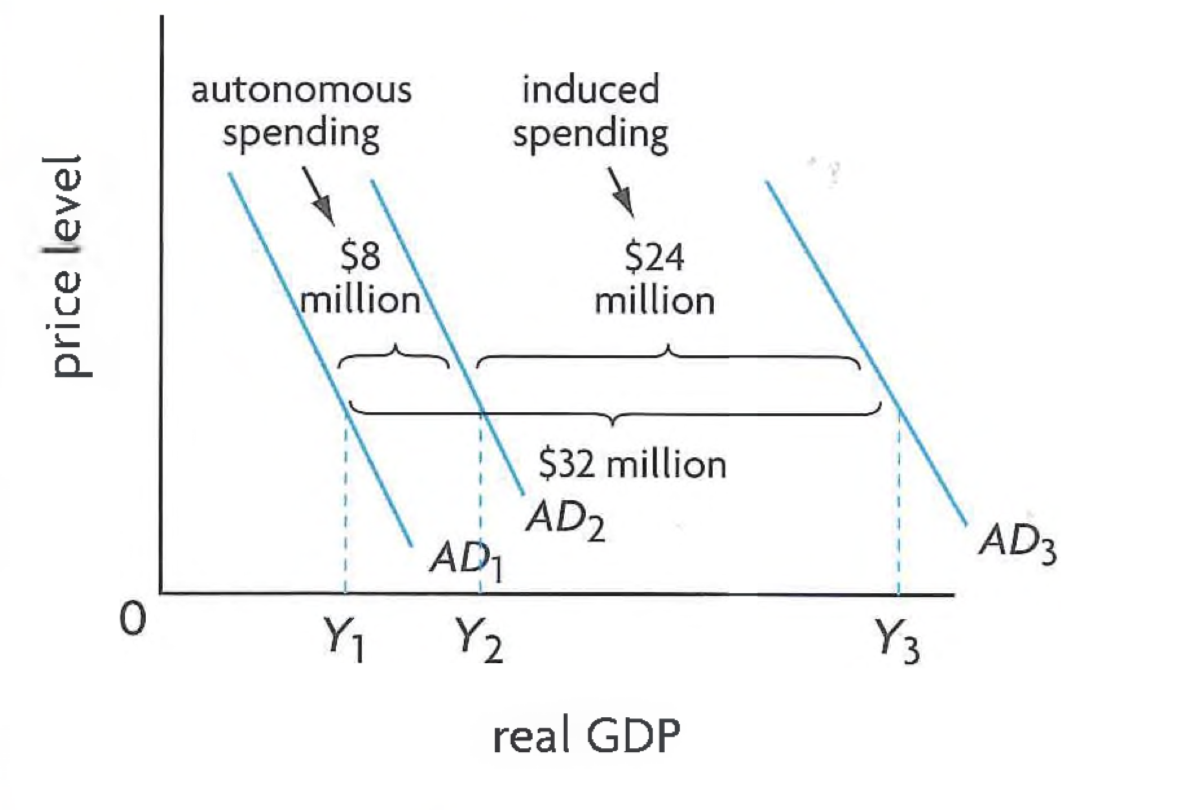
\includegraphics[width=0.5\linewidth]{Screenshot 2026-07-31 at 15.25.35.png}
\end{center}
Autonomous spending: not been caused by a change in income.\\Induced spending: caused by a change in income.\\
The multiplier effect can only be initiated by a change in spending that is not caused by a change in income.\\
In order for the multiplier to have the greatest possible effect on real GDP, it is necessary that the price level is constant. (The effect of the multiplier diminishes as AD approaches to potential output)
\subsection{Further topics on the multiplier and Keynesian economic theory }
\subsubsection*{The multiplier and fiscal policy}
The effects of fiscal policy depend on the value of the multiplier:
\begin{itemize}
  \item \textbf{Government spending increases}: the full amount enters the spending stream $\to$ multiplied impact on GDP. E.g.\ if MPC $= 3/4$, multiplier $= 4$; a \$1 increase in $G \to$ \$4 increase in AD.
  \item \textbf{Tax cuts}: less powerful than $G$ increases --- a \$1 tax cut with MPC $= 3/4$ leads to \$0.75 initial consumption increase (the remaining \$0.25 leaks out) $\to$ \$0.75 $\times$ 4 $=$ \$3 increase in AD (vs.\ \$4 from $G$).
  \item \textbf{High MPM reduces fiscal policy effectiveness}: a large fraction of additional income leaks abroad as import spending $\to$ lower MPC $\to$ smaller multiplier $\to$ weaker domestic impact.
  \item \textbf{Automatic stabilisers and the multiplier}: progressive taxes and unemployment benefits work by \textbf{reducing the MPC} $\to$ smaller multiplier $\to$ smaller induced changes in GDP $\to$ milder fluctuations. E.g.\ if unemployment benefits lower MPC from $3/4$ to $1/2$, the multiplier falls from 4 to 2.
\end{itemize}

\subsubsection*{Supplementary: Spending, tax and balanced-budget multipliers (AP Barron Ch 18)}
\begin{itemize}
  \item \needbold{Government spending multiplier}:
  \[k_G = \dfrac{1}{1-MPC} = \dfrac{1}{MPS+MPT+MPM}\]
  An increase in $G$ enters directly into aggregate demand in its entirety before generating secondary rounds of induced consumption.
  \item \needbold{Tax multiplier}:
  \[k_T = -\dfrac{MPC}{1-MPC}\]
  The tax multiplier is \textbf{negative} and \textbf{smaller in magnitude} than the spending multiplier. A tax cut of \$1 first increases disposable income by \$1, but households save a fraction ($MPS$) and spend only $MPC \times \$1$, meaning the first round of spending is smaller.
  \item \needbold{Balanced-budget multiplier}:
  \[k_{BB} = k_G + k_T = \dfrac{1}{1-MPC} + \left(-\dfrac{MPC}{1-MPC}\right) = \dfrac{1-MPC}{1-MPC} = 1\]
  When the government increases government spending and taxes by the exact same amount ($\Delta G = \Delta T$), real GDP expands by exactly the amount of the spending increase (multiplier equals 1).
\end{itemize}

\subsubsection*{The Keynesian cross model}
Jelps understand the relationship between AD and (real GDP), the idea of \textbf{less-than-full-employment equilibrium}, and the \textbf{multiplier effect}.
\\
\textbf{Key distinction}: \textbf{aggregate output (real GDP)} = sum of all \textit{actual} expenditures ($C + I + G + X - M$). \textbf{Aggregate demand} = sum of all \textit{desired} expenditures ($C + I + G + X - M$). The two are not always equal.
\\
\textbf{Consumption function}: desired consumption ($C$) depends positively on income ($Y$). The slope of the $C$ function $= \Delta C / \Delta Y =$ the \textbf{MPC}. At low income, $C > Y$ (negative saving / dissaving); at high income, $C < Y$ (positive saving).
\\
\textbf{Adding investment}: desired investment ($I$) is \textbf{autonomous} (independent of income). The $C + I$ line is parallel to the $C$ line (shifted up by a constant amount).
\\
\textbf{Equilibrium}: occurs where the \textbf{desired spending line ($C + I$)} intersects the \textbf{45$^\circ$ line} (where desired spending $=$ income $=$ real GDP). At this point, the amount buyers want to buy equals the amount produced $\to$ equilibrium output $Y_e$.
\begin{itemize}
  \item If output $< Y_e$: desired spending $>$ output $\to$ inventories sold $\to$ firms increase production $\to$ GDP rises toward $Y_e$.
  \item If output $> Y_e$: desired spending $<$ output $\to$ unsold goods accumulate $\to$ firms cut production $\to$ GDP falls toward $Y_e$.
\end{itemize}
Crucially, $Y_e$ may be \textbf{below full-employment output} $\to$ the economy can be in equilibrium with \textbf{cyclical unemployment} (a deflationary gap). This was Keynes's key insight against the classical view that the economy self-corrects to full employment.
\\
\begin{center}
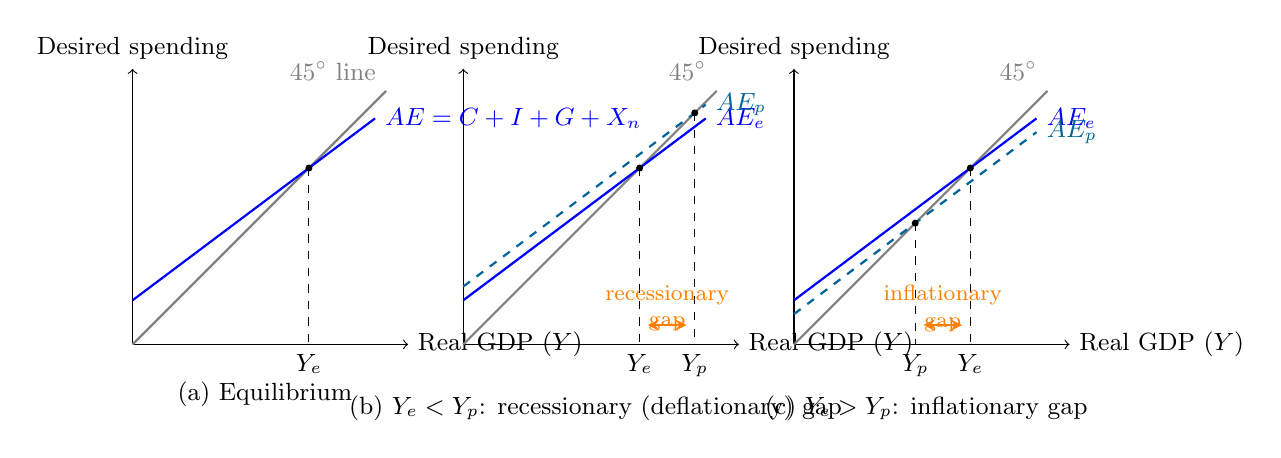
\begin{tikzpicture}[scale=0.7]
% (a) Equilibrium
\begin{scope}
\draw[->] (0,0) -- (5.0,0) node[right, font=\small] {Real GDP ($Y$)};
\draw[->] (0,0) -- (0,5.0) node[above, font=\small] {Desired spending};
\draw[thick, gray] (0,0) -- (4.6,4.6) node[above left, gray, font=\small] {45$^\circ$ line};
\draw[thick, blue] (0,0.8) -- (4.4,4.1) node[right, blue, font=\small] {$AE = C+I+G+X_n$};
\filldraw (3.2,3.2) circle (1.5pt);
\draw[dashed] (3.2,3.2) -- (3.2,0) node[below, font=\small] {$Y_e$};
\node[font=\small, align=center] at (2.4,-0.9) {(a) Equilibrium};
\end{scope}
% (b) Recessionary gap
\begin{scope}[xshift=6.0cm]
\draw[->] (0,0) -- (5.0,0) node[right, font=\small] {Real GDP ($Y$)};
\draw[->] (0,0) -- (0,5.0) node[above, font=\small] {Desired spending};
\draw[thick, gray] (0,0) -- (4.6,4.6) node[above left, gray, font=\small] {45$^\circ$};
\draw[thick, blue] (0,0.8) -- (4.4,4.1) node[right, blue, font=\small] {$AE_e$};
\draw[thick, blue!60!green, dashed] (0,1.05) -- (4.4,4.35) node[right, blue!60!green, font=\small] {$AE_p$};
\filldraw (3.2,3.2) circle (1.5pt);
\filldraw (4.2,4.2) circle (1.5pt);
\draw[dashed] (3.2,3.2) -- (3.2,0) node[below, font=\small] {$Y_e$};
\draw[dashed] (4.2,4.2) -- (4.2,0) node[below, font=\small] {$Y_p$};
\draw[<->, >=stealth, thick, orange] (3.35,0.35) -- (4.05,0.35);
\node[font=\footnotesize, orange, align=center] at (3.7,0.65) {recessionary\\gap};
\node[font=\small, align=center] at (2.4,-1.15) {(b) $Y_e < Y_p$: recessionary (deflationary) gap};
\end{scope}
% (c) Inflationary gap
\begin{scope}[xshift=12.0cm]
\draw[->] (0,0) -- (5.0,0) node[right, font=\small] {Real GDP ($Y$)};
\draw[->] (0,0) -- (0,5.0) node[above, font=\small] {Desired spending};
\draw[thick, gray] (0,0) -- (4.6,4.6) node[above left, gray, font=\small] {45$^\circ$};
\draw[thick, blue] (0,0.8) -- (4.4,4.1) node[right, blue, font=\small] {$AE_e$};
\draw[thick, blue!60!green, dashed] (0,0.55) -- (4.4,3.85) node[right, blue!60!green, font=\small] {$AE_p$};
\filldraw (2.2,2.2) circle (1.5pt);
\filldraw (3.2,3.2) circle (1.5pt);
\draw[dashed] (2.2,2.2) -- (2.2,0) node[below, font=\small] {$Y_p$};
\draw[dashed] (3.2,3.2) -- (3.2,0) node[below, font=\small] {$Y_e$};
\draw[<->, >=stealth, thick, orange] (2.35,0.35) -- (3.05,0.35);
\node[font=\footnotesize, orange, align=center] at (2.7,0.65) {inflationary\\gap};
\node[font=\small, align=center] at (2.4,-1.15) {(c) $Y_e > Y_p$: inflationary gap};
\end{scope}
\end{tikzpicture}
\end{center}
The Keynesian cross also illustrates the multiplier: an upward shift in autonomous spending (e.g.\ higher $I$ or $G$) moves the equilibrium to a \textbf{new, higher} $Y_e$, with the increase in output being a \textbf{multiple} of the initial spending change.
\subsection{Supply-side policies}
\textbf{Goals}: promote long-term growth (rightward shift of LRAS); improve competition and efficiency; reduce labour costs and unemployment through greater labour market flexibility; increase firm incentives to invest; reduce inflation to improve international competitiveness.
\\\\
Two types: \textbf{market-based} (favoured by monetarist/new classical) and \textbf{interventionist} (favoured by Keynesian economists).

\subsubsection*{Market-based supply-side policies}
\textbf{1. Encouraging competition}:
\begin{itemize}
  \item \textbf{Privatisation}: transfer public $\to$ private sector $\to$ improved efficiency/management (government enterprises often inefficient due to bureaucracy, lack of profit motive).
  \item \textbf{Deregulation}: reduce government regulation. \textit{Economic deregulation} (price/output controls, protection from competition) has been widely removed (transport, telecoms, energy). \textit{Social regulation} (consumer/worker safety, pollution) is being strengthened in many countries, though some argue it is excessive/bureaucratic.
  \item \textbf{Contracting out}: governments hire private firms to provide goods/services (IT, accounting, public goods) $\to$ increased competition.
  \item \textbf{Anti-monopoly regulation}: enforce legislation, break up large firms, prevent anti-competitive mergers.
  \item \textbf{Trade liberalisation}: reduce trade barriers $\to$ freer trade increases domestic and global competition.
\end{itemize}
\textbf{2. Labour market reforms} (increase labour market flexibility / reduce rigidities):
\begin{itemize}
  \item \textbf{Abolish/reduce minimum wage} $\to$ allow equilibrium wage to fall $\to$ lower unemployment, lower labour costs.
  \item \textbf{Weaken labour unions} $\to$ wages more responsive to supply and demand.
  \item \textbf{Reduce unemployment benefits} $\to$ increase incentive to find work $\to$ lower natural rate of unemployment.
  \item \textbf{Reduce job security} (make firing easier/cheaper) $\to$ firms more willing to hire $\to$ higher employment.
\end{itemize}
\textbf{3. Incentive-related policies} (tax cuts):
\begin{itemize}
  \item \textbf{Lower personal income taxes} $\to$ higher after-tax income $\to$ incentive to work more (more hours, more workers, delayed retirement, shorter unemployment) $\to$ LRAS shifts right.
  \item \textbf{Lower capital gains / interest income taxes} $\to$ more saving $\to$ more funds for investment $\to$ more capital goods $\to$ higher potential output.
  \item \textbf{Lower business taxes} $\to$ higher after-tax profits $\to$ more investment and R\&D $\to$ greater potential output.
\end{itemize}
\subsubsection*{Interventionist supply-side policies}
\begin{itemize}
  \item \textbf{Investment in human capital}: education, training (retraining programmes, grants, subsidies for hiring structurally unemployed, relocation assistance); improved health care access $\to$ higher labour productivity $\to$ LRAS shifts right. Positive externalities justify government intervention.
  \item \textbf{Investment in new technology (R\&D)}: government R\&D spending + incentives (tax breaks, patents) for private R\&D $\to$ new/improved capital goods $\to$ higher potential output.
  \item \textbf{Investment in infrastructure}: roads, ports, telecoms, power, irrigation $\to$ lower costs, higher efficiency, improved labour productivity $\to$ LRAS shifts right. Often merit/public goods justifying government provision.
  \item \textbf{Industrial policies}: support for \textbf{SMEs} (tax exemptions, grants, low-interest loans); support for \textbf{infant industries} in developing countries (subsidies, tariffs).
\end{itemize}
\subsubsection*{Overlaps between demand-side and supply-side policies}

\subsubsection*{Demand-side effects of supply-side policies}
\begin{itemize}
  \item \textbf{Interventionist}: government spending on education, health, R\&D, infrastructure $\to$ increases $G$ directly $\to$ AD shifts right (short-term demand-side effect) while also shifting LRAS right (long-term supply-side effect).
  \item \textbf{Market-based incentive policies}: tax cuts $\to$ higher disposable income $\to$ $C \uparrow$ and $I \uparrow$ $\to$ AD shifts right (demand-side), in addition to intended supply-side effects on LRAS.
\end{itemize}

\subsubsection*{Supply-side effects of demand-side policies}
\textbf{Fiscal policy} can affect potential output directly and indirectly:
\begin{itemize}
  \item \textbf{Direct}: government spending on infrastructure (roads, ports, telecoms), R\&D, education/training, health care $\to$ increases quantity/quality of physical and human capital $\to$ LRAS shifts right.
  \item \textbf{Indirect}: creates a stable macroeconomic environment (low inflation, low unemployment) $\to$ encourages private investment $\to$ capital formation, technological improvement.
  \item \textbf{Incentives}: lower business taxes $\to$ more investment and R\&D $\to$ new capital and innovation.
\end{itemize}
\textbf{Monetary policy}: lower interest rates $\to$ more spending on capital goods $\to$ increased quantity of physical capital $\to$ higher potential output.
\begin{center}
\begin{itemize}
  \item In practice, the distinction between short-term (demand-side) and long-term (supply-side) growth is \textbf{blurred} --- policy-makers focus on overall real GDP growth, using a mix of policies.
\end{itemize}
\end{center}

\subsubsection*{Evaluation of supply-side policies}
\textbf{Constraints on market-based policies}:
\begin{itemize}
  \item \textbf{Time lags}: effects on AS take significant time.
  \item \textbf{Possible short-term unemployment increase}: privatisation (cost-cutting/firing), deregulation (competitive pressure), contracting out (government job losses).
  \item \textbf{Negative effects on equity}: reduced worker protection (minimum wage, job security, benefits) $\to$ lower incomes, rising inequality; tax cuts benefit mainly higher-income groups; privatised firms may raise prices on necessities.
  \item \textbf{Negative impact on government budget}: tax cuts reduce revenues $\to$ deficit.
  \item \textbf{Vested interests}: unions, workers in public enterprises, firms with market power oppose reforms.
  \item \textbf{Possible negative environmental effects}: increased competition may increase negative externalities (pollution).
\end{itemize}
\textbf{Constraints on interventionist policies}:
\begin{itemize}
  \item \textbf{Time lags}: investments in human/physical capital, R\&D take time.
  \item \textbf{Negative impact on government budget}: heavy government spending $\to$ deficit.
\end{itemize}
\textbf{Strengths of market-based policies}: improved resource allocation; minimal budget burden (except tax cuts); ability to reduce natural rate of unemployment; reduce inflationary pressure (LRAS shifts right to match AD growth).
\textbf{Strengths of interventionist policies}: direct support for growth-critical sectors (infrastructure, R\&D, education); directly creates employment (skills training, relocation assistance); potential to reduce inflationary pressure; \textbf{positive effects on equity} (broadly distributed human capital investment).

\subsubsection*{Ongoing debates}
\begin{itemize}
  \item \textbf{Interventionist vs.\ market-based for potential output growth}: interventionists point to Asian Tigers (heavy government investment in human capital + industrial policy); market-based supporters argue government interference causes inefficiency/misallocation, political pressures, high taxes $\to$ disincentives.
  \item \textbf{Incentive-related policies}: questionable whether tax cuts actually increase work/saving/investment --- higher after-tax income may lead to more leisure, not work; US savings are at historic lows despite tax cuts. Supply-side effects may be small relative to demand-side effects.
  \item \textbf{Minimum wages}: market-based advocates argue for reducing minimum wage to cut unemployment; but evidence suggests higher wages can increase productivity $\to$ firms demand more labour $\to$ employment may not fall (or only falls at very high minimum wage levels).
\end{itemize}
Most economists agree policies should \textbf{complement each other}; the right mix depends on each country's conditions.

\subsection{Evaluation of policies to achieve macroeconomic objectives}
\subsubsection*{Policies for low unemployment}
\textbf{Cyclical unemployment} (caused by insufficient AD):
\begin{itemize}
  \item \textbf{Monetary policy} (expansionary): lower interest rates $\to$ higher $C$ and $I$ $\to$ AD shifts right $\to$ recessionary gap closes. \textit{Pros}: incremental, reversible, short lags, no political constraints, no crowding out/debt. \textit{Cons}: may be ineffective in deep recession (zero lower bound, low confidence, banks fearful of lending).
  \item \textbf{Fiscal policy} (expansionary): increase $G$ / cut taxes $\to$ AD shifts right. \textit{Pros}: can pull economy out of deep recession; $G$ impacts AD directly; can target specific sectors (infrastructure $\to$ also supply-side effects); automatic stabilisers lessen severity. \textit{Cons}: time lags; cannot fine-tune; budget deficit $\to$ debt $\to$ possible crowding out.
  \item \textbf{Supply-side policies}: market-based policies do not help cyclical unemployment (they affect AS, not AD). Interventionist policies \textit{can} help (they have demand-side effects via increased $G$).
\end{itemize}
\textbf{Natural unemployment} (structural, frictional, seasonal):
\begin{itemize}
  \item \textbf{Demand-side policies are generally not appropriate}: increasing AD when at potential output only causes inflation (temporarily lowers unemployment below natural rate, but it returns).
  \item \textbf{Interventionist supply-side}: retraining programmes, grants/loans for education, subsidies for hiring structurally unemployed, relocation assistance, job information centres/websites $\to$ reduce structural, frictional and seasonal unemployment. \textit{Pros}: direct positive impact without worsening inequality/job security. \textit{Cons}: budget burden, opportunity costs.
  \item \textbf{Market-based supply-side}: labour market reforms (reduce minimum wage, weaken unions, reduce job security, reduce unemployment benefits). \textit{Pros}: reduce natural rate without budget burden. \textit{Cons}: worsen income inequality and worker protection.
\end{itemize}

\subsubsection*{Policies for a low and stable rate of inflation}
\textbf{Demand-pull inflation} (caused by excess AD):
\begin{itemize}
  \item \textbf{Monetary policy} (contractionary): raise interest rates $\to$ lower $C$ and $I$ $\to$ AD shifts left. \textit{Pros}: incremental, reversible, short lags, no political constraints. \textit{Cons}: may conflict with external balance (higher interest rates $\to$ currency appreciation $\to$ exports less competitive, imports cheaper $\to$ worsens trade deficit).
  \item \textbf{Fiscal policy} (contractionary): cut $G$ / raise taxes $\to$ AD shifts left. \textit{Pros}: spending cuts have direct AD impact; automatic stabilisers help. \textit{Cons}: highly unpopular politically; cumbersome; time lags.
  \item \textbf{Supply-side policies}: cannot address short-term demand-pull inflation (long time lags), but over the long term, shifting LRAS right keeps inflationary pressures under control as potential output grows to match AD.
\end{itemize}
\textbf{Cost-push inflation} (caused by rising costs / supply-side shocks):
\begin{itemize}
  \item \textbf{Demand-side policies are problematic}: inflation requires lowering AD, but unemployment requires raising AD $\to$ \textbf{conflict}. Central banks committed to low inflation use contractionary monetary policy at the cost of more recession and unemployment. Fiscal policy generally not used.
  \item \textbf{Supply-side policies}: no general solution; depends on the cause:
  \begin{itemize}
    \item \textit{Wage increases}: labour market reforms (lower minimum wage, weaken unions).
    \item \textit{Imported input price increases} (e.g.\ oil): develop alternative energy, encourage conservation $\to$ reduce demand for oil $\to$ lower price (long-term policy).
    \item \textit{Firms with market power}: break up monopolies/oligopolies, encourage competition.
    \item \textit{Currency depreciation raising import prices}: reduce import dependence (``expenditure-switching'' policies; see Chapter 17 HL).
  \end{itemize}
\end{itemize}

\subsubsection*{Policies to promote economic growth}
\begin{itemize}
  \item \textbf{Short-term growth} (increases in AD within the LRAS): expansionary \textbf{monetary} and \textbf{fiscal} policies.
  \item \textbf{Long-term growth} (rightward shifts of LRAS): \textbf{supply-side policies} (both interventionist and market-based) --- investment in human capital, R\&D, infrastructure, industrial policies; plus market-based reforms (competition, labour market flexibility, tax incentives).
  \item In practice the distinction is \textbf{blurred}: demand-side policies have supply-side effects (e.g.\ fiscal spending on infrastructure) and supply-side policies have demand-side effects (e.g.\ increased $G$ on education). Policy-makers use a \textbf{mix} and focus on overall real GDP growth.
  \item If in a deflationary gap: expansionary demand-side policies (+ interventionist supply-side). As the economy approaches potential output: supply-side policies become more important (to avoid inflation by increasing productive capacity alongside AD).
  \item Each policy must be evaluated on its own strengths and weaknesses (see above sections) and selected according to the country's particular circumstances.
\end{itemize}
\newpage
% ------------------------------------------------------------
\section*{Unit 4 The Global Economy}
\section{International trade: Part I}
\subsection{The benefits of international trade}
\needbold{Free trade}: the absence of government intervention of any kind in international trade.
\begin{itemize}
  \item \textbf{Increased competition}: imports and exports expose domestic firms to foreign competition $\to$ forces firms to become more efficient.
  \item \textbf{Greater efficiency in production}: firms must produce at lowest possible cost to compete; higher-cost firms lose sales and may go out of business.
  \item \textbf{Lower prices for consumers}: greater competition + efficiency + imports of cheaper foreign goods $\to$ lower prices.
  \item \textbf{Greater choice for consumers}: trade allows import of a larger variety of goods/services, possibly of higher quality.
  \item \textbf{Acquiring needed resources}: countries import natural resources, capital goods, and inputs not available domestically (e.g.\ oil, timber, minerals, machinery).
  \item \textbf{Source of foreign exchange}: exports earn foreign currencies $\to$ enables payments for imports and other foreign payments.
  \item \textbf{Access to larger markets}: firms are not limited by domestic market size; exports expand potential sales.
  \item \textbf{Economies of scale}: access to larger markets allows firms to grow beyond national boundaries $\to$ lower average costs $\to$ lower prices and greater export competitiveness.
  \item \textbf{Increased domestic production and consumption through specialisation}: a country specialises in goods it produces efficiently $\to$ produces more of these, trades for goods produced more cheaply elsewhere $\to$ greater total output and consumption (basis of \textbf{comparative advantage} theory).
  \item \textbf{More efficient allocation of resources}: free trade + specialisation $\to$ less waste of scarce resources $\to$ more efficient resource allocation both within countries and globally.
  \item \textbf{Flow of new ideas and technology}: as G\&S flow between countries, new ideas, technologies and skills are transferred.
  \item \textbf{Reduced possibility of hostilities}: strong trade links create economic interdependence $\to$ reduces likelihood of war (e.g.\ the EEC/EU was created partly to prevent future Franco-German wars).
  \item \textbf{Trade as an ``engine for growth''}: all the above factors contribute to increases in domestic output and economic growth.
\end{itemize}
\begin{center}
  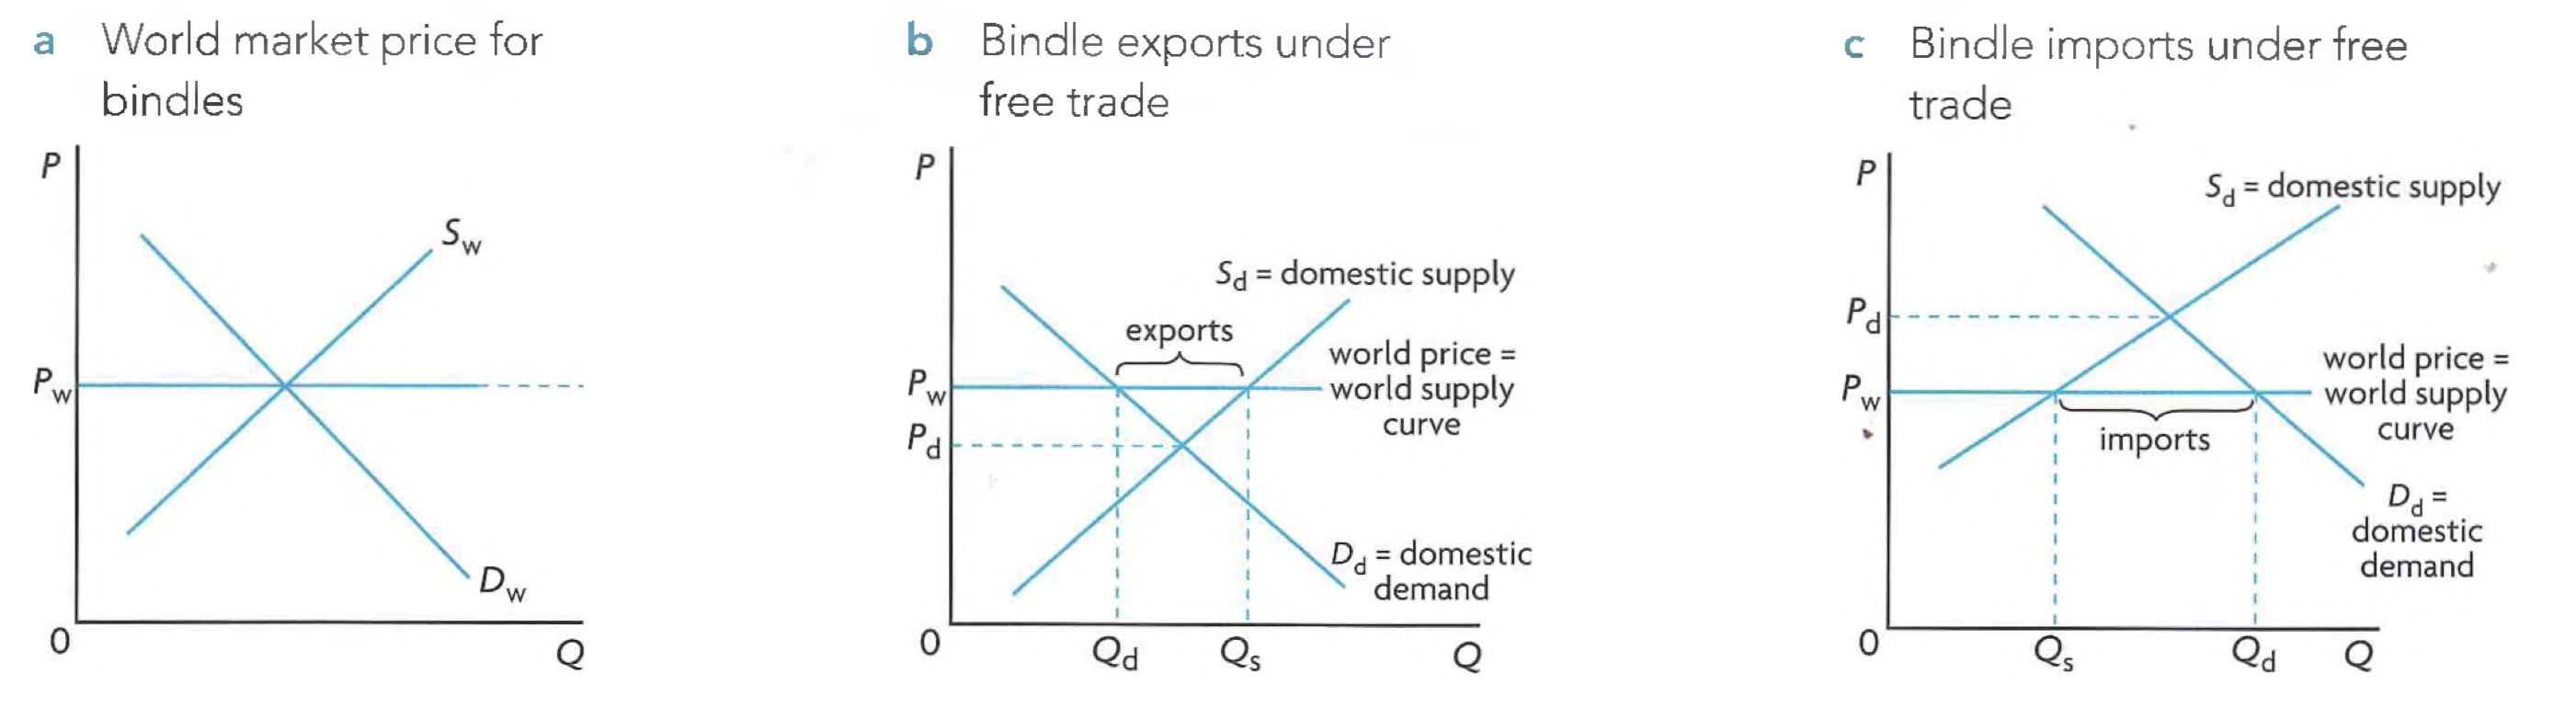
\includegraphics[width=0.9\linewidth]{Screenshot 2026-07-31 at 16.29.51.png}
\end{center}
Bindles: good produced by many countries around the world, allowed for free trade.\\
The world bindle price is determined by world demand and world supply, where world demand is the sum of all country demands and world supply is the sum of all country supplies. \\\\
Whether the goods should be exported / imported depends on the domestic price relative to the world price. 
\begin{itemize}
  \item \textbf{Domestic price $>$ world price}: domestic producers cannot compete with cheaper foreign goods $\to$ imports are encouraged; domestic consumers benefit from lower prices.
  \item \textbf{Domestic price $<$ world price}: domestic producers can sell at higher prices abroad $\to$ exports are encouraged; domestic producers benefit from higher prices.
\end{itemize}
Note that the world supply curve is perfectly elastic.
\subsubsection*{Calculation}
Quantities exported / imported is determined by the difference between domestic supply and domestic demand at the world price. \\
Export revenue / import expenditure = world price $\times$ quantity exported / imported.\\
For consumers, they are worse off in case of exports and better off in case of imports. \\
For producers, they are better off in case of exports and worse off in case of imports.\\
\textbf{Effects on surplus (supplementary, recommended for HL)}: with trade, the changes in producer surplus (PS), consumer surplus (CS) and social surplus can be calculated from the domestic demand and supply curves at the world price $P_w$:
\begin{itemize}
  \item \textbf{Exporting country}: producer revenue rises (larger quantity at the higher world price) $\to$ \textbf{PS rises}; consumers pay more and buy less $\to$ \textbf{CS falls}. The gain in PS \textbf{exceeds} the loss in CS by triangle $X$ (between the world price and the autarky price, over the extra exported quantity), so \textbf{social surplus rises}.
  \item \textbf{Importing country}: consumers pay less and buy more $\to$ \textbf{CS rises}; producers receive less and sell less $\to$ \textbf{PS falls}. The gain in CS \textbf{exceeds} the loss in PS by triangle $X$, so \textbf{social surplus rises}.
\end{itemize}
\begin{center}
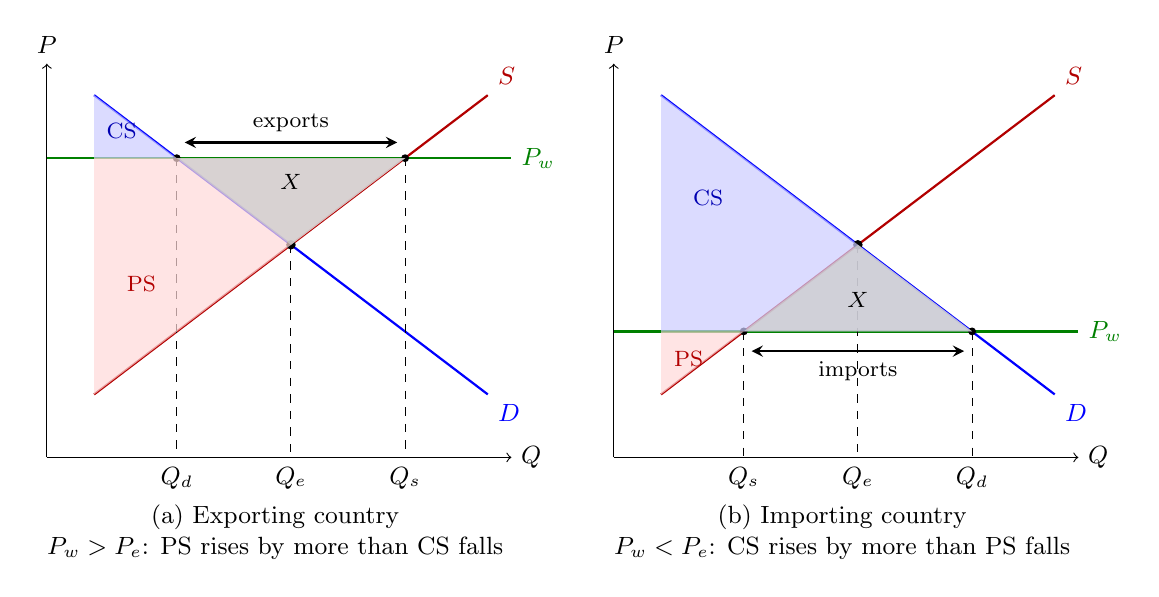
\begin{tikzpicture}[scale=1.0]
% (a) Exporting country
\begin{scope}
\draw[->] (0,0) -- (5.9,0) node[right, font=\small] {$Q$};
\draw[->] (0,0) -- (0,5.0) node[above, font=\small] {$P$};
\draw[thick, blue] (0.6,4.6) -- (5.6,0.8) node[below right, blue, font=\small] {$D$};
\draw[thick, red!70!black] (0.6,0.8) -- (5.6,4.6) node[above right, red!70!black, font=\small] {$S$};
\draw[thick, green!50!black] (0,3.8) -- (5.9,3.8) node[right, green!50!black, font=\small] {$P_w$};
\filldraw (3.1,2.7) circle (1.5pt);
\filldraw (1.65,3.8) circle (1.2pt);
\filldraw (4.55,3.8) circle (1.2pt);
\draw[dashed] (1.65,3.8) -- (1.65,0) node[below, font=\small] {$Q_d$};
\draw[dashed] (4.55,3.8) -- (4.55,0) node[below, font=\small] {$Q_s$};
\draw[dashed] (3.1,2.7) -- (3.1,0) node[below, font=\small] {$Q_e$};
\fill[blue!20, opacity=0.7] (0.6,4.6) -- (1.65,3.8) -- (0.6,3.8) -- cycle;
\node[blue!70!black, font=\footnotesize] at (0.95,4.15) {CS};
\fill[red!15, opacity=0.7] (0.6,0.8) -- (4.55,3.8) -- (0.6,3.8) -- cycle;
\node[red!70!black, font=\footnotesize] at (1.2,2.2) {PS};
\fill[gray!40, opacity=0.75] (1.65,3.8) -- (4.55,3.8) -- (3.1,2.7) -- cycle;
\node[font=\footnotesize] at (3.1,3.5) {$X$};
\draw[<->, >=stealth, thick] (1.75,4.0) -- (4.45,4.0);
\node[font=\footnotesize] at (3.1,4.25) {exports};
\node[font=\small, align=center] at (2.9,-0.95) {(a) Exporting country\\ $P_w > P_e$: PS rises by more than CS falls};
\end{scope}
% (b) Importing country
\begin{scope}[xshift=7.2cm]
\draw[->] (0,0) -- (5.9,0) node[right, font=\small] {$Q$};
\draw[->] (0,0) -- (0,5.0) node[above, font=\small] {$P$};
\draw[thick, blue] (0.6,4.6) -- (5.6,0.8) node[below right, blue, font=\small] {$D$};
\draw[thick, red!70!black] (0.6,0.8) -- (5.6,4.6) node[above right, red!70!black, font=\small] {$S$};
\draw[thick, green!50!black] (0,1.6) -- (5.9,1.6) node[right, green!50!black, font=\small] {$P_w$};
\filldraw (3.1,2.7) circle (1.5pt);
\filldraw (1.65,1.6) circle (1.2pt);
\filldraw (4.55,1.6) circle (1.2pt);
\draw[dashed] (1.65,1.6) -- (1.65,0) node[below, font=\small] {$Q_s$};
\draw[dashed] (4.55,1.6) -- (4.55,0) node[below, font=\small] {$Q_d$};
\draw[dashed] (3.1,2.7) -- (3.1,0) node[below, font=\small] {$Q_e$};
\fill[blue!20, opacity=0.7] (0.6,4.6) -- (4.55,1.6) -- (0.6,1.6) -- cycle;
\node[blue!70!black, font=\footnotesize] at (1.2,3.3) {CS};
\fill[red!15, opacity=0.7] (0.6,0.8) -- (1.65,1.6) -- (0.6,1.6) -- cycle;
\node[red!70!black, font=\footnotesize] at (0.95,1.25) {PS};
\fill[gray!40, opacity=0.75] (1.65,1.6) -- (4.55,1.6) -- (3.1,2.7) -- cycle;
\node[font=\footnotesize] at (3.1,2.0) {$X$};
\draw[<->, >=stealth, thick] (1.75,1.35) -- (4.45,1.35);
\node[font=\footnotesize] at (3.1,1.1) {imports};
\node[font=\small, align=center] at (2.9,-0.95) {(b) Importing country\\ $P_w < P_e$: CS rises by more than PS falls};
\end{scope}
\end{tikzpicture}
\end{center}
In both cases, trade raises social welfare relative to autarky; the only difference is \textbf{who gains}: with exports, producers gain at the expense of consumers; with imports, consumers gain at the expense of producers.
\subsection{Free trade: absolute and comparative advantage}
\subsubsection*{The theory of absolute advantage}
\needbold{Absolute advantage} refers to the ability of one country to produce a good using fewer resources than another country. Putting it differently, a country has an absolute advantage in a good if with the same quantity of resources it can produce more of the good than another country.\\\\
The determination of absolute advantage is only based on the number of goods produced, rather than comparing with OPC.\\
If countries specialise in the producing the goods that has absolute advantage, the result will be that whereas both countries will be producing somewhere on their PPC, due to specialisation and trade they can consume at a point outside their PPC.
\subsubsection*{The theory of relative advantage}
\needbold{Comparative advantage} refers to the situation where one country has a lower opportunity cost (relative cost) in the production of a good than another country.\\
Ricardo showed that countries can gain from specialisation and trade even if one country has an absolute advantage in both goods.\\
\textbf{Example: output per worker per day}
\begin{center}
\begin{tabular}{lcc}
\toprule
& \textbf{Country A} & \textbf{Country B} \\
\midrule
Wheat (tonnes) & 6 & 2 \\
Cloth (metres) & 3 & 2 \\
\bottomrule
\end{tabular}
\end{center}
Country A has an absolute advantage in both goods (6 $>$ 2 for wheat; 3 $>$ 2 for cloth). However, comparative advantage depends on \textbf{opportunity cost}:

\begin{center}
\begin{tabular}{lcc}
\toprule
\textbf{Opportunity cost of 1 unit} & \textbf{Country A} & \textbf{Country B} \\
\midrule
1 tonne of wheat & $\frac{3}{6} = 0.5$ m cloth & $\frac{2}{2} = 1$ m cloth \\
1 metre of cloth & $\frac{6}{3} = 2$ t wheat & $\frac{2}{2} = 1$ t wheat \\
\bottomrule
\end{tabular}
\end{center}
\begin{itemize}
  \item Country A has a \textbf{lower OPC} in wheat (0.5 $<$ 1) $\to$ \textbf{comparative advantage in wheat}.
  \item Country B has a \textbf{lower OPC} in cloth (1 $<$ 2) $\to$ \textbf{comparative advantage in cloth}.
\end{itemize}
\[OPC=\dfrac{\text{Sacrifice of one good}}{\text{Gain of one good}}\]
A country has a comparative advantage in the production of the good that has a lower opportunity cost (lower relative cost). \\
If A specialises in wheat and B specialises in cloth, total output increases and both countries can \textbf{consume beyond their PPC} through trade. \\\\
According to the theory (or law) of comparative advantage, as long as opportunity costs in two (or more) countries differ, it is possible for all countries to gain from specialisation and trade according to their comparative advantage. \\\\
For 2 countries with parallel PPCs, there's no meaning of trade since the OPC for producing the two goods are the same for these two countries.
\subsubsection*{Sources of comparative advantage}
Comparative advantage arises from differences in \textbf{factor endowments} --- the quantity and quality of factors of production (land, labour, capital, entrepreneurship) plus technology. Examples:
\begin{itemize}
  \item \textbf{Climate/geography}: temperate vs.\ tropical countries differ in agricultural comparative advantage (coffee/cocoa grow in tropics; wheat in temperate zones).
  \item \textbf{Physical geography}: mountainous countries are less suited to agriculture; landlocked countries cannot easily produce shipping services (Greece $\to$ shipping + tourism; Switzerland $\to$ precision watches/clocks).
  \item \textbf{Labour quality and quantity}: education, skills, health of the workforce.
  \item \textbf{Capital and technology}: countries with advanced technology have comparative advantage in high-tech/manufactured goods.
\end{itemize}

\subsubsection*{Strengths and limitations of the theory of comparative advantage}
\textbf{Strength}: the key conclusion --- that free trade increases global production and consumption, leading to improved global resource allocation --- forms the justification for the global trend toward \textbf{trade liberalisation} since the early 1990s.
\\\\
\textbf{Limitations --- unrealistic assumptions}:
\begin{itemize}
  \item \textbf{Factors of production are fixed}: in reality, labour and capital move between countries; quality changes over time (education, skills) $\to$ factor endowments and comparative advantage \textit{change}.
  \item \textbf{Technology is fixed}: new technologies continuously emerge $\to$ comparative advantage shifts.
  \item \textbf{Perfect mobility of FoPs within the country}: switching production from one good to another is assumed instant and costless; in reality, switching costs may be so high as to change comparative advantage.
  \item \textbf{Full employment of resources}: countries are assumed to produce on their PPCs; but many countries (especially developing ones) have high unemployment/underemployment $\to$ comparative advantage differs from the full-employment case.
  \item \textbf{Free trade}: in reality, governments intervene heavily in trade (tariffs, quotas, subsidies).
  \item \textbf{Homogeneous products}: all units of a good are assumed identical; in reality, products are differentiated.
  \item \textbf{Transportation costs ignored}: real transport costs change relative prices and may limit gains from specialisation.
\end{itemize}
\textbf{Structural changes may be blocked}: as economies grow, the agricultural sector shrinks while manufacturing and services grow (especially in developing countries). If countries specialise according to current comparative advantage, they may be locked into producing the same goods $\to$ \textbf{structural changes cannot occur} (e.g.\ an agricultural economy cannot industrialise).
\\\\
\textbf{Excessive specialisation}: if a country has comparative advantage in only one/few products, over-specialisation makes it \textbf{vulnerable} to global recessions, falling export prices, or fluctuating primary product prices $\to$ unstable export revenues and economic decline.

\subsection{Supplementary: Terms of trade (Edexcel Book 2 Ch 25)}
The \needbold{terms of trade (ToT)} measures the rate of exchange of one country's exports for another country's imports, expressed as the ratio of an export price index to an import price index:
\[\text{ToT index} = \dfrac{\text{Index of export prices}}{\text{Index of import prices}} \times 100\]
\begin{itemize}
  \item \textbf{Improvement in terms of trade}: occurs when the ToT index increases ($> 100$ relative to the base year). Export prices rise faster than import prices (or fall more slowly). A given volume of exports can purchase a \textbf{larger volume of imports}.
  \item \textbf{Deterioration (worsening) in terms of trade}: occurs when the ToT index decreases ($< 100$). Import prices rise faster than export prices. A given volume of exports purchases a \textbf{smaller volume of imports}.
  \item \textbf{Causes of changes in ToT}:
  \begin{itemize}
    \item Changes in global demand for or supply of exports and imports.
    \item Exchange rate movements: currency appreciation makes exports more expensive in foreign currency and imports cheaper, improving the ToT; depreciation worsens the ToT.
    \item Relative inflation rates: higher domestic inflation raises export prices relative to import prices.
    \item Tariffs and trade protection.
  \end{itemize}
  \item \textbf{Consequences}:
  \begin{itemize}
    \item An improvement driven by stronger export demand raises national income and improves the current account. However, if caused by domestic inflation, export competitiveness may suffer in the long run.
    \item \textbf{Prebisch--Singer thesis}: primary commodity exporters face a long-term decline in their terms of trade because world demand for manufactured goods grows faster than demand for agricultural products and raw materials (low YED of primary commodities). Developing nations must export ever-greater volumes of commodities to buy the same quantity of manufactured capital imports.
  \end{itemize}
  \item \textbf{Worked calculation example}:
  \begin{itemize}
    \item In the base year, $\text{Export Price Index} = 100$ and $\text{Import Price Index} = 100 \implies \text{ToT} = \frac{100}{100} \times 100 = 100$.
    \item In year 2, export prices rise 10\% to 110, while import prices rise 20\% to 120:
    \[\text{ToT}_2 = \dfrac{110}{120} \times 100 \approx 91.7\]
    Because $91.7 < 100$, terms of trade deteriorated by $100 - 91.7 = 8.3\%$.
    \item In year 3, export prices increase to 121 while import prices remain at 120:
    \[\text{ToT}_3 = \dfrac{121}{120} \times 100 \approx 100.8\]
    Because $100.8 > 100$, terms of trade improved by 0.8\% relative to the base year.
    \item Percentage change formula: $\dfrac{\text{ToT}_2 - \text{ToT}_1}{\text{ToT}_1} \times 100$.
  \end{itemize}
\end{itemize}

\subsection{Types of trade protection: restrictions on free trade}
In contrast to free trade, trade protection involves government intervention in international trade through the imposition of trade restrictions (barriers) to prevent the free entry of imports into a country.
\begin{itemize}
  \item \needbold{Tariffs}: taxes on imports, which protect domestic industry from foreign competition and raise government revenue.
  \begin{center}
    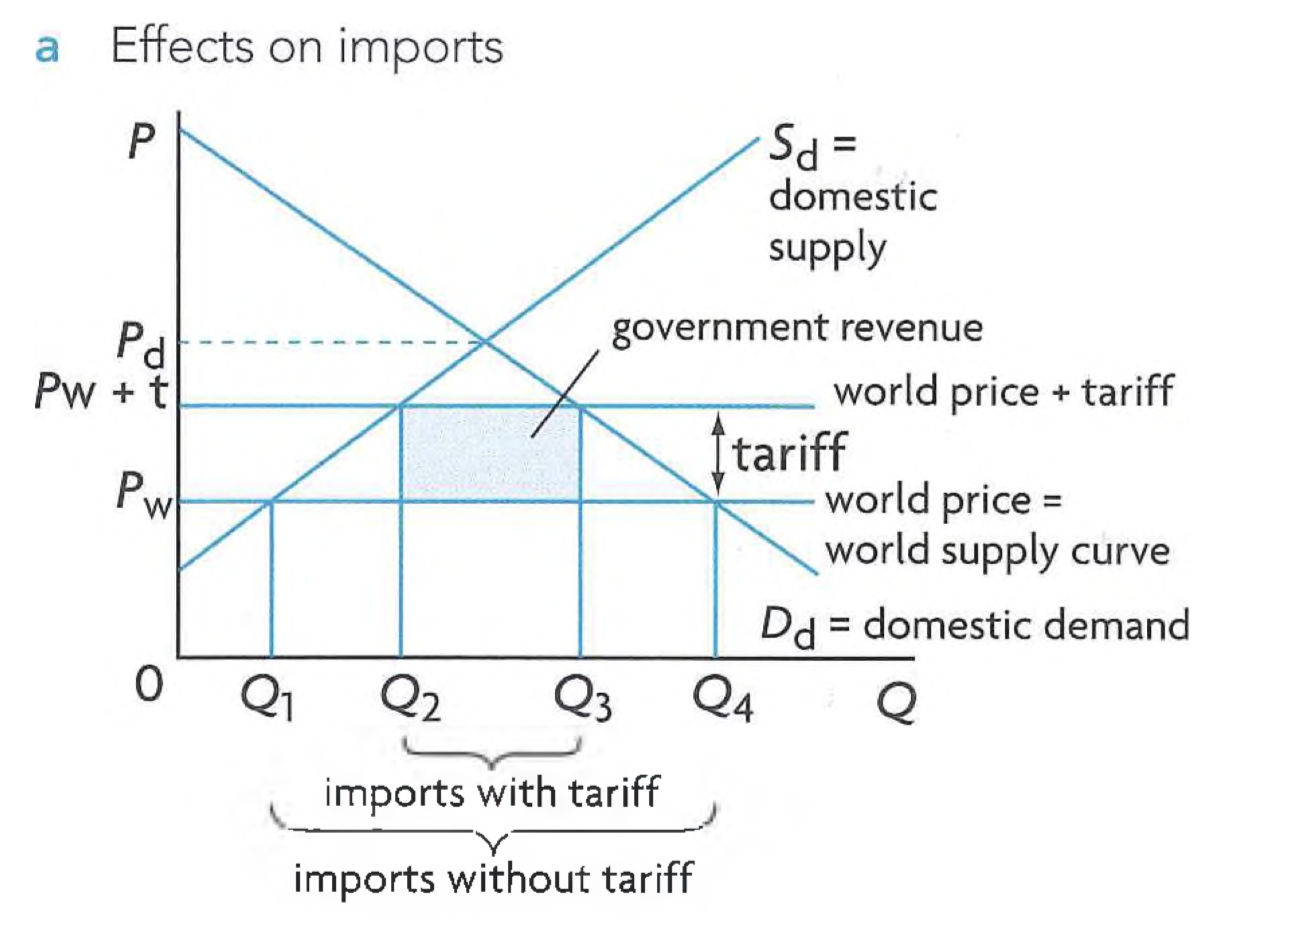
\includegraphics[width=0.45\linewidth]{Screenshot 2026-08-04 at 21.20.29.png}
    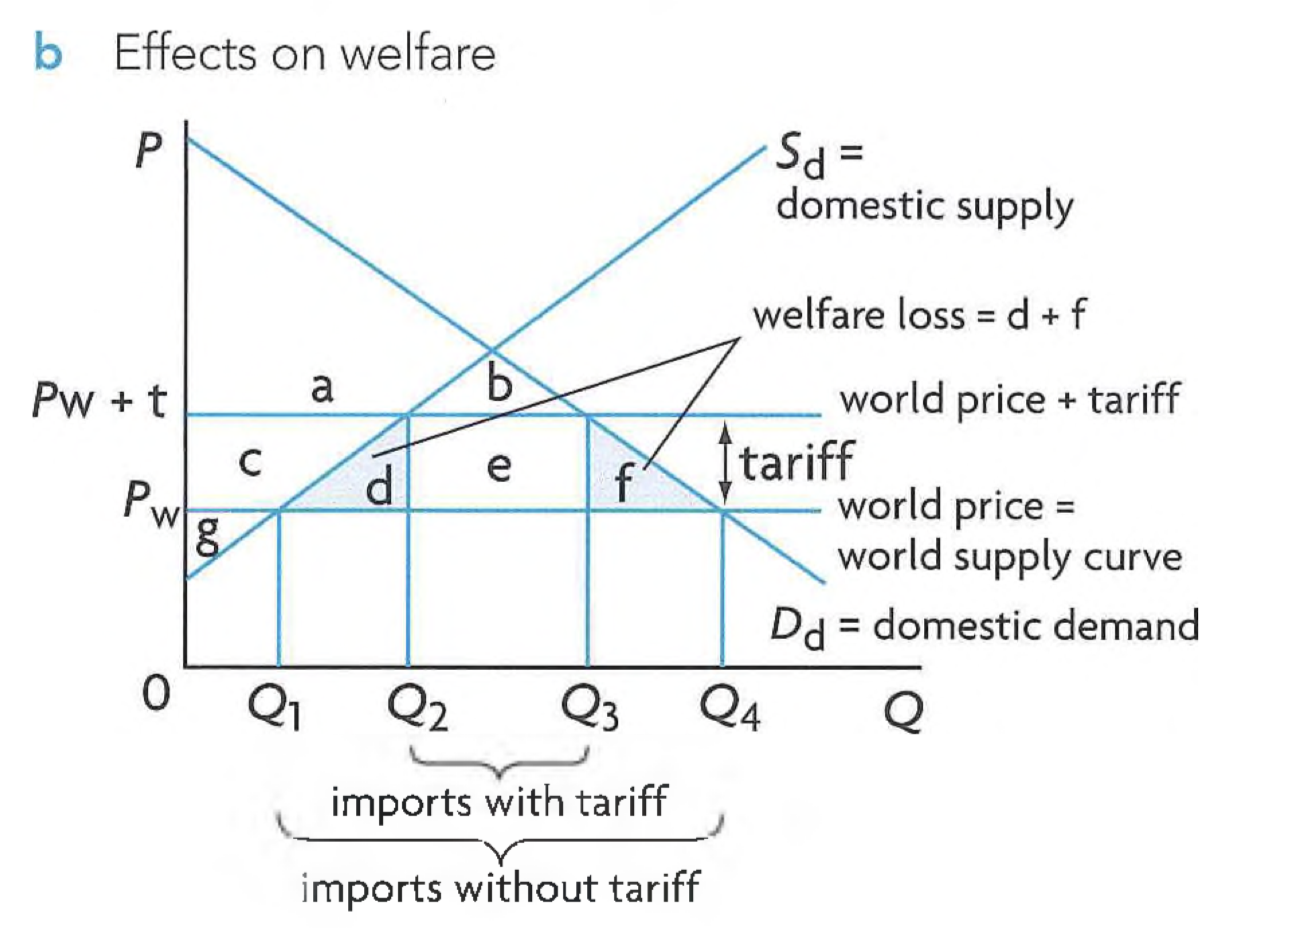
\includegraphics[width=0.45\linewidth]{Screenshot 2026-08-04 at 21.20.35.png}
  \end{center}
  \begin{itemize}
    \item \textbf{Winners}:
    \begin{itemize}
      \item \textbf{Domestic producers}: receive a higher price ($P_{w}+t$) and sell a larger quantity ($Q_s$ instead of $Q_{sw}$) $\to$ higher revenue and profit.
      \item \textbf{Domestic employment} in the protected industry increases (more output $\to$ more workers needed).
      \item \textbf{Government}: gains \textbf{tariff revenue} $= \text{tariff per unit} \times \text{quantity of imports}$ (transferred from consumers who pay $P_{w}+t$).
    \end{itemize}
    \item \textbf{Losers}:
    \begin{itemize}
      \item \textbf{Domestic consumers}: pay a \textbf{higher price} ($P_{w}+t$) and can only buy a \textbf{smaller quantity} ($Q_d$ instead of $Q_{dw}$) $\to$ loss of consumer surplus.
      \item \textbf{Domestic income distribution worsens}: the tariff acts as a \textbf{regressive tax} --- lower-income consumers pay a proportionately larger share of their income.
      \item \textbf{Inefficiency in production}: the increase in domestic output comes from \textbf{relatively inefficient} domestic producers (who couldn't compete at $P_w$) $\to$ waste of scarce resources.
      \item \textbf{Foreign producers}: export a \textbf{smaller quantity} at the same world price $P_w$ $\to$ lose export revenue.
      \item \textbf{Global misallocation of resources}: production shifts from efficient foreign producers to inefficient domestic producers; consumption falls $\to$ deadweight \textbf{welfare loss} both domestically and globally.
    \end{itemize}
    \item \textbf{Welfare loss}: the combined loss of consumer surplus exceeds the combined gains of producer surplus + government revenue; the remainder is the \textbf{deadweight welfare loss} (two triangles: one from production inefficiency, one from consumption loss).
    \item \textbf{Calculation of tariff revenue}: $\text{Tariff revenue} = (P_{w}+t - P_w) \times (Q_d - Q_s)$ (quantity after implementation of tariff). \\
    (Note here that import expenditures after the tariff are calculated using $P_w$ rather than $P_w+t$)
  \end{itemize}
  \item \needbold{Import quotas}: a legal limit to the quantity of a good that can be imported over a particular time period (typically a year). \\The effects are similar compared to that of tariffs, except that it doesn't generate government revenue.
  \begin{center}
    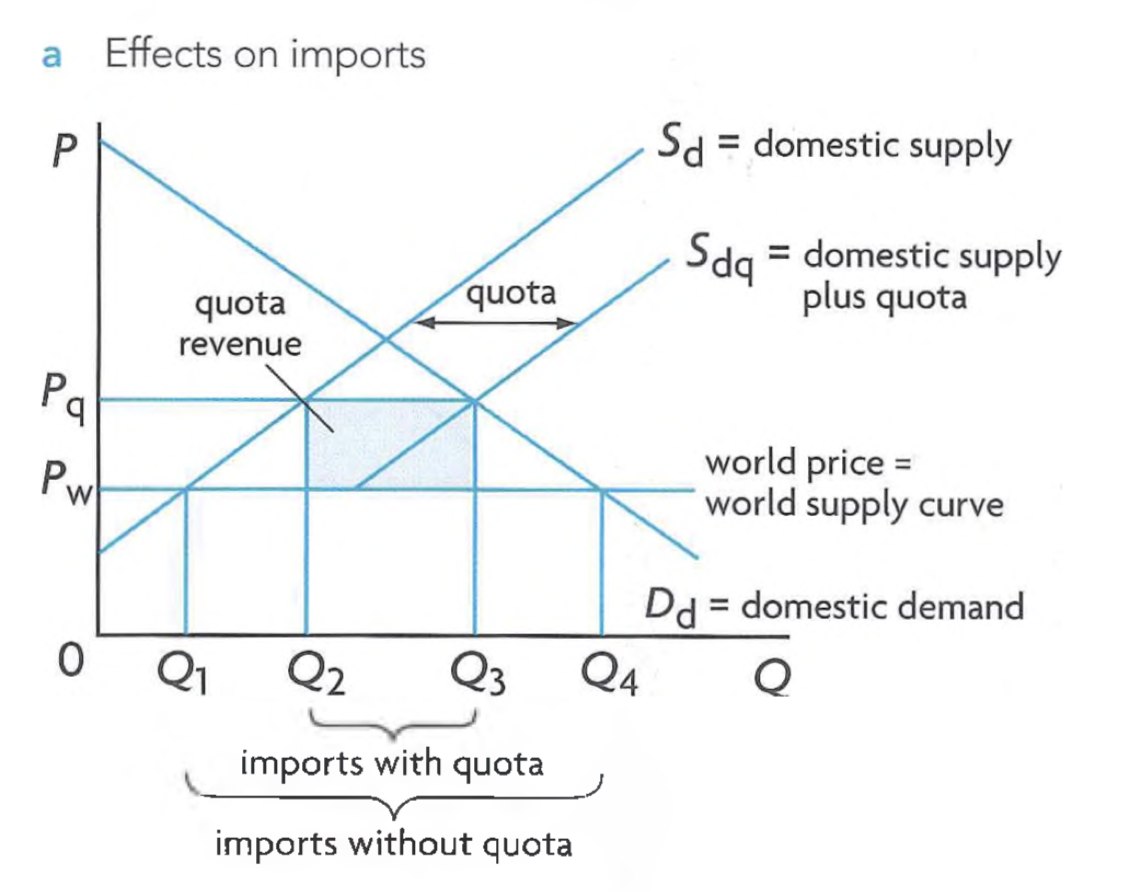
\includegraphics[width=0.45\linewidth]{Screenshot 2026-08-05 at 19.35.21.png}
    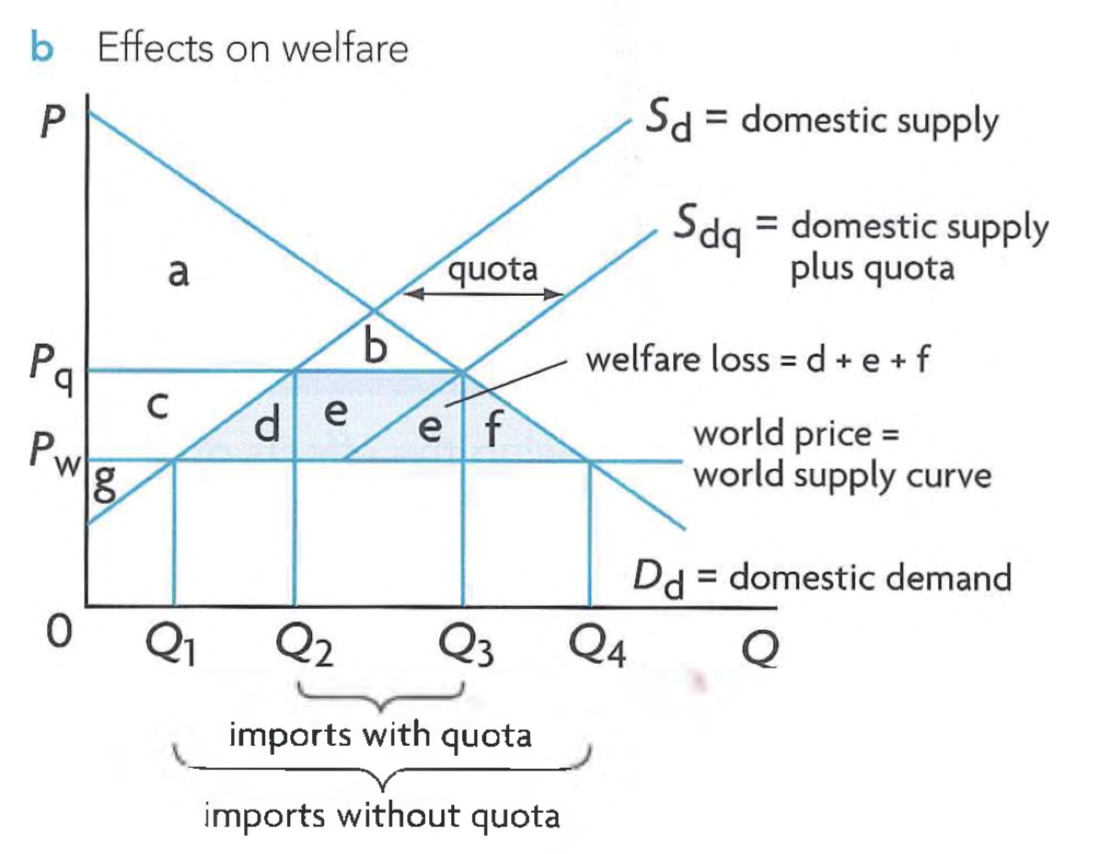
\includegraphics[width=0.45\linewidth]{Screenshot 2026-08-05 at 19.35.34.png}
  \end{center}
  When the government sets a quota, it issues a limited number of import licences determining the legal limit on the quantity of imports. The holders of these licences are the only individuals with the legal right to import. These licence holders gain quota revenues (buy at $P_w$ and sell at $P_q$). 
  \begin{itemize}
    \item \textbf{Winners}:
    \begin{itemize}
      \item \textbf{Domestic producers}: receive a higher price ($P_q$) and sell a larger quantity $\to$ higher revenue and profit.
      \item \textbf{Domestic employment} in the protected industry increases.
    \end{itemize}
    \item \textbf{Neutral impact}:
    \begin{itemize}
      \item \textbf{Government} neither gains nor loses --- import licences are usually given to foreign governments, so no quota revenue is collected by the domestic government.
    \end{itemize}
    \item \textbf{Losers}:
    \begin{itemize}
      \item \textbf{Domestic consumers}: pay a \textbf{higher price} ($P_q$) for a \textbf{smaller quantity} $\to$ loss of consumer surplus.
      \item \textbf{Domestic income distribution worsens}: the price increase ($P_q - P_w$) acts like a \textbf{regressive tax} --- lower-income consumers pay a proportionately larger share.
      \item \textbf{Inefficiency in production}: increased output by relatively inefficient domestic producers $\to$ waste of resources.
      \item \textbf{Exporting countries}: export a smaller quantity (lose export revenue) but \textit{gain} quota revenues (if they receive the import licences). Net effect depends on which is larger --- loss of export revenue vs.\ gain of quota revenue.
      \item \textbf{Global misallocation of resources}: consumption falls; production shifts from efficient foreign to inefficient domestic producers $\to$ welfare loss.
    \end{itemize}
  \end{itemize}
  \item \needbold{Production subsidies}: payments per unit of output granted by the government to domestic firms that compete with imports. The subsidy shifts the domestic supply curve \textbf{downward (rightward)}; domestic firms expand output, imports fall.
  \begin{center}
    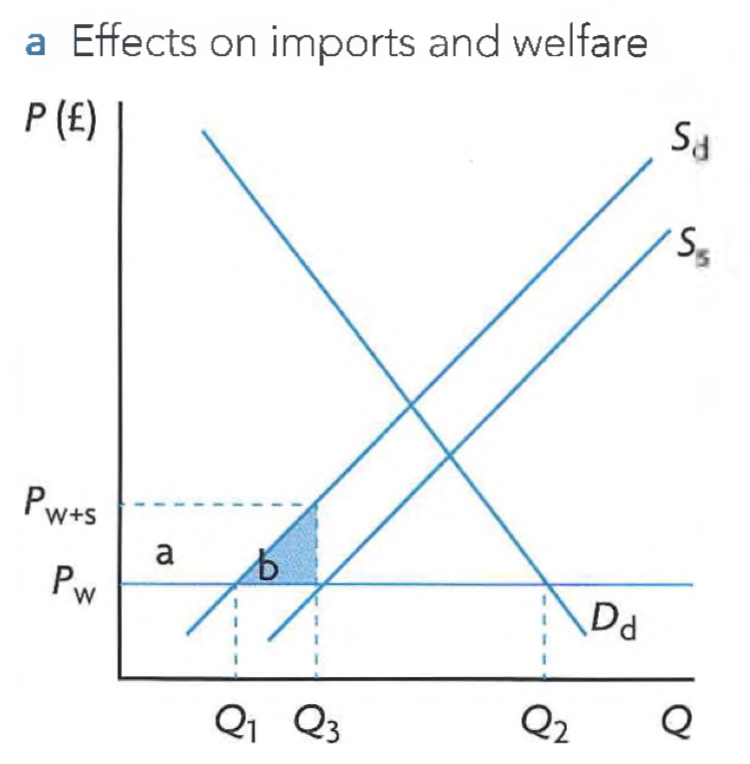
\includegraphics[width=0.3\linewidth]{Screenshot 2026-08-05 at 19.58.05.png}
  \end{center}
  Government has a welfare loss / subsidy cost = a + b.
  \begin{itemize}
    \item \textbf{Winners}:
    \begin{itemize}
      \item \textbf{Domestic producers}: receive $P_{w+s}$ ($= P_w$ + subsidy per unit) and produce a larger quantity $\to$ higher revenue and profit.
      \item \textbf{Domestic employment} in the protected industry increases.
    \end{itemize}
    \item \textbf{Neutral impact}:
    \begin{itemize}
      \item \textbf{Consumers are not affected}: consumption and price remain at $Q_2$ and $P_w$ (consumers buy more domestic output and less imports, but total quantity and price are unchanged).
    \end{itemize}
    \item \textbf{Losers}:
    \begin{itemize}
      \item \textbf{Government budget}: must spend tax revenue on the subsidy $= (P_{w+s} - P_w) \times Q_s'$ (subsidy per unit $\times$ quantity produced domestically after subsidy).
      \item \textbf{Taxpayers}: tax revenue diverted to subsidising inefficient producers $\to$ opportunity cost (funds could have been spent on merit goods, etc.).
      \item \textbf{Inefficiency in production}: output by relatively inefficient domestic producers increases while more efficient foreign producers lose market share.
      \item \textbf{Exporting countries}: export a smaller quantity $\to$ lose export revenue.
      \item \textbf{Global misallocation of resources}: production shifts from efficient to inefficient producers $\to$ welfare loss.
    \end{itemize}
    \item \textbf{Advantage over tariffs/quotas}: consumers are not harmed (no higher price, no reduced quantity); only a \textbf{production-side} distortion.
  \end{itemize}
  \item \needbold{Export subsidies}: Export subsidies are similar to production subsidies in that they involve a payment by the government per unit of the subsidised good, except that now the subsidy is paid for each unit of the good that is exported. 
  \begin{center}
    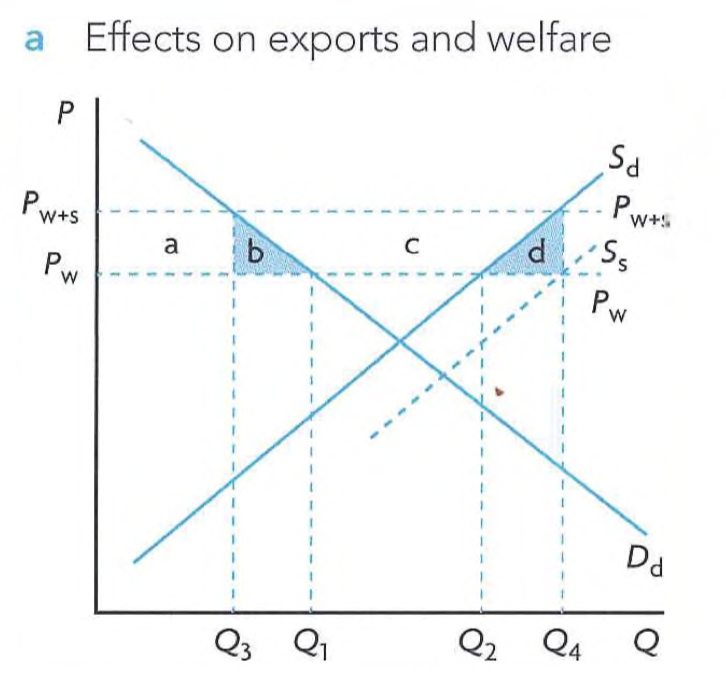
\includegraphics[width=0.3\linewidth]{Screenshot 2026-08-05 at 20.05.06.png}
  \end{center}
  Exported volume increases from $Q_2-Q_1$ to $Q_4-Q_3$ (Supply shifted rightward, find that the price level of the point moved upward from $P_w$ intersecting with $S_s$ of $P_{w+s}$, while the world (exported) price remains $P_w$.) (Government gives b + c + d to domestic producers for the exported products)
  \begin{itemize}
    \item \textbf{Winners}:
    \begin{itemize}
      \item \textbf{Domestic producers}: receive a higher price ($P_{w+s}$) and sell a larger quantity $\to$ higher revenue and profit; export volume increases.
      \item \textbf{Domestic employment} in the export industry increases.
    \end{itemize}
    \item \textbf{Losers}:
    \begin{itemize}
      \item \textbf{Domestic consumers}: must pay a \textbf{higher price} ($P_{w+s}$) and consume a \textbf{smaller quantity} $\to$ loss of consumer surplus.
      \item \textbf{Government budget}: must finance the subsidy $= (P_{w+s} - P_w) \times \text{quantity of exports}$.
      \item \textbf{Taxpayers}: subsidy is financed by tax revenue $\to$ opportunity cost (funds diverted from alternative uses such as merit goods).
      \item \textbf{Domestic income distribution worsens}: the price increase ($P_{w+s} - P_w$) is \textbf{regressive} --- hurts lower-income consumers proportionately more.
      \item \textbf{Inefficiency in production}: inefficient domestic producers are protected by the artificially higher price.
      \item \textbf{Foreign producers (exporting countries)}: lose global market share to subsidised exports $\to$ falling export revenues.
      \item \textbf{Global misallocation of resources}: increased inefficiency in resource allocation worldwide.
    \end{itemize}
    \item \textbf{Note}: export subsidies can have \textbf{very serious negative effects} globally, as they distort world markets and harm foreign producers who cannot compete with artificially cheap subsidised exports.
  \end{itemize}
\end{itemize}
\section{International trade: Part II}
\subsection{Arguments for and against trade protection}
\subsubsection*{Arguments economists justify under certain conditions}
\begin{itemize}
  \item \textbf{Infant industry argument}: new domestic industries have not yet achieved EOS and cannot compete with mature foreign firms $\to$ need \textbf{temporary} protection until they grow large enough to compete. Strongest theoretical argument (Hamilton, 1791; used mainly by developing countries). \textit{Dangers}: hard to identify which industries have potential; protected firms may lack incentive to become efficient; governments may not remove protection after maturation.
  \item \textbf{National security}: certain industries (aircraft, weapons, chemicals, minerals) are essential for defence $\to$ should not depend on imports. \textit{Non-economic argument} --- decisions should be political/military, but hard to draw the line (steel, candles, umbrellas have all claimed ``national security'' protection).
  \item \textbf{Health, safety and environmental standards}: imported goods must meet domestic standards. \textit{Risk}: standards may be used as ``hidden protection'' to keep out competing goods (administrative barriers).
  \item \textbf{Diversification in developing countries}: ELDCs are often over-specialised in a few primary commodities $\to$ excessive specialisation is risky. Trade protection can help diversify into new industries. \textit{Risk}: governments may not know which industries to select.
\end{itemize}
\subsubsection*{Arguments economists find questionable}
\begin{itemize}
  \item \textbf{Anti-dumping}: \needbold{dumping} = selling below cost in foreign markets (usually via export subsidies). Anti-dumping tariffs/quotas may be justified, but the argument is often \textbf{abused} as an excuse to protect domestic producers since proving dumping is difficult and time-consuming.
  \item \textbf{Unfair competition}: includes dumping, production/export subsidies, administrative barriers, undervalued currencies, intellectual property violations. \textit{Same problem}: hard to prove $\to$ easily abused as pretext for protection.
  \item \textbf{Correcting a balance of payments deficit}: tariffs/quotas reduce imports $\to$ less outward payment. \textit{Problem}: invites retaliation; only a short-term emergency measure; better long-term solutions exist (Chapters 16--17).
  \item \textbf{Tariffs as government revenue}: common in developing countries (easy to collect at borders). \textit{Problems}: regressive tax $\to$ worsens income distribution; allocative inefficiency; may delay broader tax reform. Should be temporary and gradually phased out.
  \item \textbf{Protection of domestic jobs}: import restrictions increase domestic production/employment. \textit{Problems}: (i) if protected goods are inputs for other industries, higher input prices $\to$ lower production and \textit{increased} unemployment elsewhere (may exceed gains); (ii) retaliation from exporting countries; (iii) fiscal/monetary/supply-side policies or targeted subsidies are better tools for employment.
\end{itemize}

\subsubsection*{Arguments against trade protection}
\textbf{Summary of stakeholder impacts} (all five protection types):
\begin{center}
\renewcommand{\arraystretch}{1.3}
\footnotesize
\begin{tabular}{lccccc}
\toprule
\textbf{Stakeholder} & \textbf{Tariff} & \textbf{Quota} & \textbf{Prod.\ sub.} & \textbf{Export sub.} & \textbf{Admin.\ barr.} \\
\midrule
Producers & gain & gain & gain & gain & gain \\
Workers & gain & gain & gain & gain & gain \\
Government & gain & neutral & lose & lose & neutral \\
Taxpayers & neutral & neutral & lose & lose & neutral \\
Consumers & lose & lose & neutral & lose & lose \\
Producer efficiency & lose & lose & lose & lose & lose \\
Income distribution & lose & lose & neutral & lose & lose \\
Resource alloc.\ (dom.) & lose & lose & lose & lose & lose \\
Foreign producers & lose & lose & lose & lose & lose \\
Global resource alloc. & lose & lose & lose & lose & lose \\
\bottomrule
\end{tabular}
\end{center}
\textbf{Key points from the table}:
\begin{itemize}
  \item Producers and workers are the \textbf{only} universal winners.
  \item Consumers lose in almost all cases (except production subsidies, where price/quantity are unchanged).
  \item Foreign producers lose in \textbf{all} cases.
  \item Domestic and global resource allocation worsens in \textbf{all} cases.
  \item Consumer losses generally \textbf{exceed} producer gains (welfare loss).
\end{itemize}
\textbf{Additional negative effects on the broader economy}:
\begin{itemize}
  \item \textbf{Cost-push inflation}: protected goods used as inputs (e.g.\ textiles, fertiliser) raise costs for downstream industries $\to$ SRAS shifts left $\to$ higher prices, lower real GDP, higher unemployment.
  \item \textbf{Reduced export competitiveness}: if protected inputs are used in exported goods, higher domestic costs $\to$ less competitive exports.
  \item \textbf{Trade wars / retaliation}: one country's barriers invite retaliatory barriers $\to$ chain reaction $\to$ declining global output and trade.
  \item \textbf{Corruption}: import restrictions create opportunities for bribes, smuggling, and misappropriated tariff revenues.
\end{itemize}
\subsection{Economic integration: trading blocs}
A \textbf{trading bloc} is a group of countries that have agreed to reduce tariff and other barriers to trade for the purpose of encouraging free or freer trade and co-operation between them.

\textbf{Preferential trade agreements (PTAs)}: agreements between countries to lower trade barriers on particular products between members; barriers remain on non-members. PTAs can be \textbf{bilateral} (two countries), \textbf{regional} (a geographic group), or \textbf{multilateral} (WTO, involving many countries worldwide).
\\\\
\textbf{Degrees of economic integration} (from lowest to highest):
\begin{itemize}
  \item \textbf{Free trade area (FTA)}: members eliminate tariffs/quoters among themselves but each retains \textbf{independent trade policies} toward non-members. Requires ``rules of origin'' to prevent non-members exploiting lower internal barriers. Examples: NAFTA/USMCA, ASEAN Free Trade Area.
  \item \textbf{Customs union}: FTA + \textbf{common external tariff} on non-members. No rules of origin needed; members act as a group in trade negotiations. Examples: CEFTA, SACU. \textit{Challenge}: members must co-ordinate policies toward non-members, which may lead to disagreements.
  \item \textbf{Common market}: customs union + \textbf{free movement of factors of production} (labour and capital). Example: EEC (1957, precursor to EU), CARICOM. \textit{Advantages}: free trade benefits + resource mobility + greater investment. \textit{Challenge}: requires significant co-ordination (migration policy, labour standards, etc.).
\end{itemize}
\textbf{Trade creation vs.\ trade diversion}:
\begin{itemize}
  \item \textbf{Trade creation}: formation of a trading bloc causes a member to \textbf{replace higher-cost domestic production} with \textbf{lower-cost imports} from another member $\to$ greater efficiency, lower prices, higher consumption, increased social welfare.
  \item \textbf{Trade diversion}: a member shifts imports from a \textbf{lower-cost non-member} to a \textbf{higher-cost member} (because the member's goods are now tariff-free) $\to$ less efficient allocation, reduced welfare.
  \item Overall welfare improves only if \textbf{trade creation $>$ trade diversion}. Trade diversion cannot occur under multilateral (WTO) liberalisation --- an argument in favour of WTO over regional blocs.
\end{itemize}
\textbf{Benefits of trading blocs}:
\begin{itemize}
  \item \textbf{Trade creation}: replacement of higher-cost domestic production with lower-cost imports from members $\to$ greater efficiency, lower prices, higher consumption, increased welfare.
  \item \textbf{Increased competition}: removal of barriers forces domestic firms to compete with lower-cost member producers $\to$ improved efficiency, lower prices, better resource allocation.
  \item \textbf{Expansion into larger markets}: firms can sell beyond national boundaries $\to$ increased exports and sales.
  \item \textbf{Economies of scale}: larger markets allow firms to grow $\to$ lower average costs.
  \item \textbf{Lower prices and greater consumer choice}: elimination of barriers + increased competition + EOS $\to$ lower prices; increased imports $\to$ greater variety.
  \item \textbf{Increased investment}: enlarged markets attract both internal investment and \textbf{FDI} from non-member firms wanting to access the bloc.
\end{itemize}
\textbf{Disadvantages of trading blocs}:
\begin{itemize}
  \item \textbf{Trade diversion}: imports shift from a \textbf{lower-cost non-member} to a \textbf{higher-cost member} (because member goods are now tariff-free) $\to$ less efficient allocation, reduced welfare.
  \item \textbf{Reduced multilateral trade}: trading blocs may divert trade away from non-members, reducing global trade liberalisation efforts (WTO).
  \item \textbf{Loss of sovereignty}: members must co-ordinate trade policies (especially customs unions and common markets) $\to$ lose independence in setting tariffs, regulations and policies.
  \item \textbf{Unequal distribution of gains}: benefits may be uneven --- larger/more developed members may gain disproportionately; smaller members may lose industries or face increased competition.
  \item \textbf{Administrative costs}: ``rules of origin'' in FTAs create complex bureaucratic procedures.
  \item \textbf{Risk of retaliation}: non-members may impose retaliatory barriers against the bloc.
\end{itemize}
\subsection{Economic integration: monetary union}
\textbf{Monetary union}: the highest degree of integration --- member countries adopt a \textbf{common currency} and a \textbf{common central bank} responsible for monetary policy. Example: the \textbf{European Monetary Union} (euro zone) --- 19 EU countries adopted the euro (1999); national currencies were locked at fixed exchange rates and then abandoned (2002--03).
\subsection{World Trade Organization}
The \textbf{WTO} (established 1995, successor to GATT 1947; 164 members in 2019) is the international organisation responsible for \textbf{liberalising trade}.
\\\textbf{Objectives and functions}:
\begin{itemize}
  \item \textbf{Administers WTO trade agreements} (implementation and administration).
  \item \textbf{Forum for trade negotiations} between members.
  \item \textbf{Handles trade disputes} (legal rulings based on trade agreements).
  \item \textbf{Monitors national trade policies} (periodic reviews; members must notify changes).
  \item \textbf{Technical assistance and training} for developing countries.
  \item \textbf{Co-operation with other international organisations} (IMF, World Bank).
\end{itemize}
\textbf{Core principles} (from GATT): \textbf{non-discrimination} (cannot favour one member over another); gradual \textbf{elimination of non-tariff barriers}; consultations to resolve disputes.
\\\\
\textbf{Criticisms and challenges}:
\begin{itemize}
  \item \textbf{Unfavourable treatment of developing countries}: developed countries received larger tariff cuts; non-tariff/hidden barriers against developing country exports were insufficiently addressed; agricultural subsidies in developed countries not reduced; intellectual property protection raised technology costs for developing countries.
  \item \textbf{Inability to agree on agricultural protection and services}: the \textbf{Doha Development Round} (2001) collapsed in 2008 due to developed countries refusing to cut farmer protection. One success: 2015 agreement to \textbf{phase out export subsidies}.
  \item \textbf{No distinction between developed and developing economies}: all countries treated equally (except Least Developed Countries) $\to$ unfair to developing countries that need policy flexibility.
  \item \textbf{Unequal bargaining power}: powerful countries dominate agenda-setting and negotiations; weaker members give in out of fear of retaliation; coalitions further entrench wealthy-country power. Calls for reform of the decision-making process.
  \item \textbf{Fragmentation of global trade}: growing tendency toward bilateral/regional agreements outside the WTO; rising protectionism (e.g.\ US trade policies since 2018) threatens the multilateral trading system.
\end{itemize}
\textbf{Key successes}: prevented return to full-scale protectionism during the 2008 financial crisis; agreement on phasing out export subsidies (2015); information technology tariff cuts; dispute resolution mechanism (e.g.\ US meat labelling case, 2015).

\subsection{Supplementary: Globalisation (Edexcel Book 2 Ch 21--22)}
\needbold{Globalisation} refers to the deepening economic integration and growing interdependence between national economies across the globe, characterised by increasing cross-border flows of goods, services, finance, technology, and labour.
\begin{itemize}
  \item \textbf{Key drivers of globalisation}:
  \begin{itemize}
    \item \textbf{Trade liberalisation}: reductions in tariffs and removal of non-tariff barriers under the GATT and WTO.
    \item \textbf{Transport revolutions}: containerisation, modern maritime shipping, and lower air freight costs dramatically reducing geographical distance.
    \item \textbf{Information and communication technologies (ICT)}: the internet, telecommunications, and digital platforms enabling instantaneous financial transfers and cross-border service trade.
    \item \textbf{Financial deregulation}: dismantling capital controls and liberalising foreign exchange markets.
    \item \textbf{Multinational corporations (MNCs)}: expansion of global value chains and foreign direct investment (FDI).
  \end{itemize}
  \item \textbf{Economic benefits}:
  \begin{itemize}
    \item Expanded global markets, greater exploitation of economies of scale, and enhanced comparative advantage gains.
    \item Lower prices, higher quality, and wider variety of goods and services for consumers.
    \item Accelerated transfer of technology, management expertise, and foreign capital to developing nations.
  \end{itemize}
  \item \textbf{Costs and challenges}:
  \begin{itemize}
    \item \textbf{Structural unemployment and regional decline}: manufacturing workers in advanced economies face job losses from lower-cost foreign competition.
    \item \textbf{Rising within-country inequality}: skilled workers benefit disproportionately from global integration, while unskilled workers face downward wage pressure.
    \item \textbf{Tax competition and ``race to the bottom''}: multinational firms exploit tax havens, undermining national tax bases and environmental regulations.
    \item \textbf{Financial contagion}: cross-border financial integration increases vulnerability to external financial crises (e.g.\ 2008 global financial crisis).
  \end{itemize}
\end{itemize}

\section{Exchange rates and the balance of payments}
\subsection{Floating exchange rates}
International transactions involve the use of different national currencies, known as foreign exchange.\\
These national currencies are traded for each other in the foreign exchange market, where currencies are bought and sold.\\\\
The demand for foreign currencies generates a supply of domestic currency; and demand for the domestic currency generates a supply of foreign currencies.\\\\
\needbold{Exchange rate}: the value of one currency expressed in terms of another.\\\\
In a floating exchange rate system (also known as flexible exchange rate system), exchange rates are determined by market forces, or the forces of demand and supply, with no government or central bank intervention in the foreign exchange market.
\begin{itemize}
  \item An increase in the value of a currency (such as the dollar) in a floating exchange rate system is called an appreciation.
  \item A fall in the value of a currency (the dollar) in a floating exchange rate system is called a depreciation. 
\end{itemize}
\begin{center}
  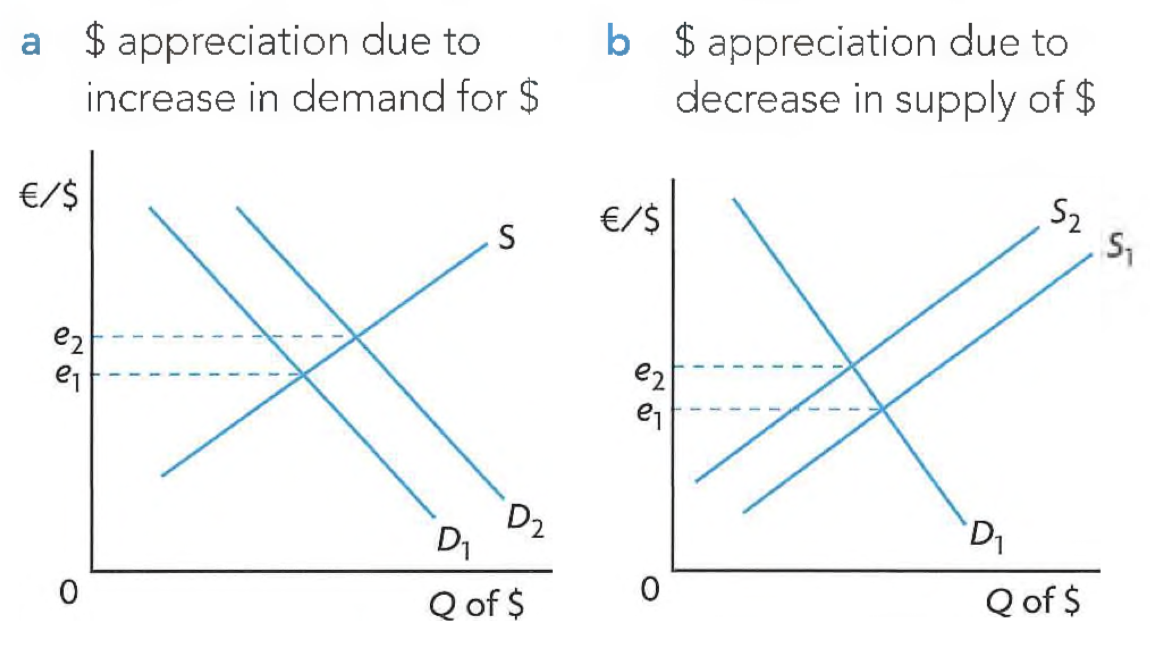
\includegraphics[width=0.45\linewidth]{Screenshot 2026-08-06 at 12.59.06.png}
  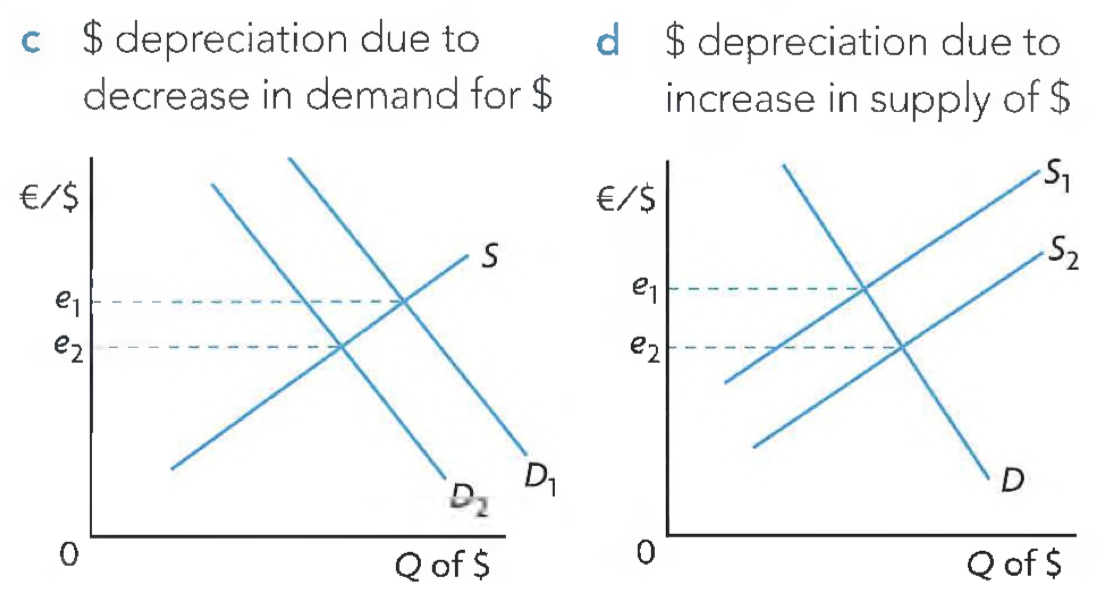
\includegraphics[width=0.45\linewidth]{Screenshot 2026-08-06 at 12.59.11.png}
\end{center}

\subsubsection*{Causes of changes in exchange rates}
\textbf{Factors affecting currency \textit{demand} (inflows of funds $\to$ appreciation)}:
\begin{itemize}
  \item \textbf{Exports of goods}: higher foreign demand for a country's exports $\to$ demand for currency rises $\to$ \textbf{appreciation}; lower export demand $\to$ depreciation.
  \item \textbf{Exports of services (tourism)}: more foreign tourists $\to$ demand for currency rises $\to$ appreciation; fewer tourists $\to$ depreciation.
  \item \textbf{Relative inflation rate}: lower inflation than trading partners $\to$ exports become relatively cheaper $\to$ higher demand for exports $\to$ appreciation. Higher relative inflation $\to$ depreciation.
  \item \textbf{Relative growth rates abroad}: higher growth in trading partners $\to$ rising incomes $\to$ more demand for exports $\to$ appreciation. Recession abroad $\to$ depreciation.
  \item \textbf{Inward FDI and portfolio investment}: more foreign investment (factories, stocks, bonds) $\to$ demand for currency rises $\to$ appreciation; less inward investment $\to$ depreciation.
  \item \textbf{Relative interest rates}: higher domestic interest rates $\to$ more attractive to foreign investors $\to$ capital inflow $\to$ demand rises $\to$ appreciation. Lower rates $\to$ depreciation. Expectations of rate changes can have the same effect.
  \item \textbf{Inward remittances}: more money sent home by workers abroad $\to$ demand for currency rises $\to$ appreciation; fewer remittances $\to$ depreciation.
  \item \textbf{Speculation (expected appreciation)}: speculators buy the currency expecting it to rise $\to$ demand increases $\to$ \textbf{self-fulfilling} appreciation.
  \item \textbf{Central bank buying}: central bank buys domestic currency (sells foreign reserves) $\to$ demand rises $\to$ appreciation.
\end{itemize}
\textbf{Factors affecting currency \textit{supply} (outflows of funds $\to$ depreciation)}:
\begin{itemize}
  \item \textbf{Imports of goods}: higher demand for imports $\to$ must buy foreign currency $\to$ supply of domestic currency rises $\to$ \textbf{depreciation}; lower imports $\to$ appreciation.
  \item \textbf{Imports of services (outbound tourism)}: more domestic tourists travelling abroad $\to$ supply of currency rises $\to$ depreciation; fewer outbound tourists $\to$ appreciation.
  \item \textbf{Relative inflation rate}: higher inflation than partners $\to$ imports become relatively cheaper $\to$ more imports $\to$ supply rises $\to$ depreciation (reinforces the export demand effect). Lower relative inflation $\to$ appreciation.
  \item \textbf{Relative growth rates (domestic)}: higher domestic growth $\to$ rising incomes $\to$ more imports $\to$ supply rises $\to$ depreciation. Lower growth $\to$ appreciation.
  \item \textbf{Outward FDI and portfolio investment}: more investment abroad $\to$ supply of currency rises $\to$ depreciation; less outward investment $\to$ appreciation.
  \item \textbf{Relative interest rates}: lower domestic rates $\to$ capital flows out $\to$ supply rises $\to$ depreciation. Higher rates $\to$ less outflow $\to$ appreciation (reinforces the demand effect).
  \item \textbf{Outward remittances}: more money sent abroad by foreign workers $\to$ supply rises $\to$ depreciation; fewer $\to$ appreciation.
  \item \textbf{Speculation (expected depreciation)}: speculators sell the currency expecting it to fall $\to$ supply increases $\to$ \textbf{self-fulfilling} depreciation.
  \item \textbf{Central bank selling}: central bank sells domestic currency (buys foreign reserves) $\to$ supply rises $\to$ depreciation.
\end{itemize}
\textbf{When both demand and supply change simultaneously}:
\begin{itemize}
  \item \textbf{Relative inflation}: lower domestic inflation $\to$ export demand rises \textit{and} import demand falls $\to$ \textbf{both} push toward appreciation (double effect).
  \item \textbf{Relative interest rates}: higher domestic rates $\to$ demand for currency rises (inflow) \textit{and} supply falls (less outflow) $\to$ \textbf{both} push toward appreciation (double effect).
\end{itemize}
\begin{center}
  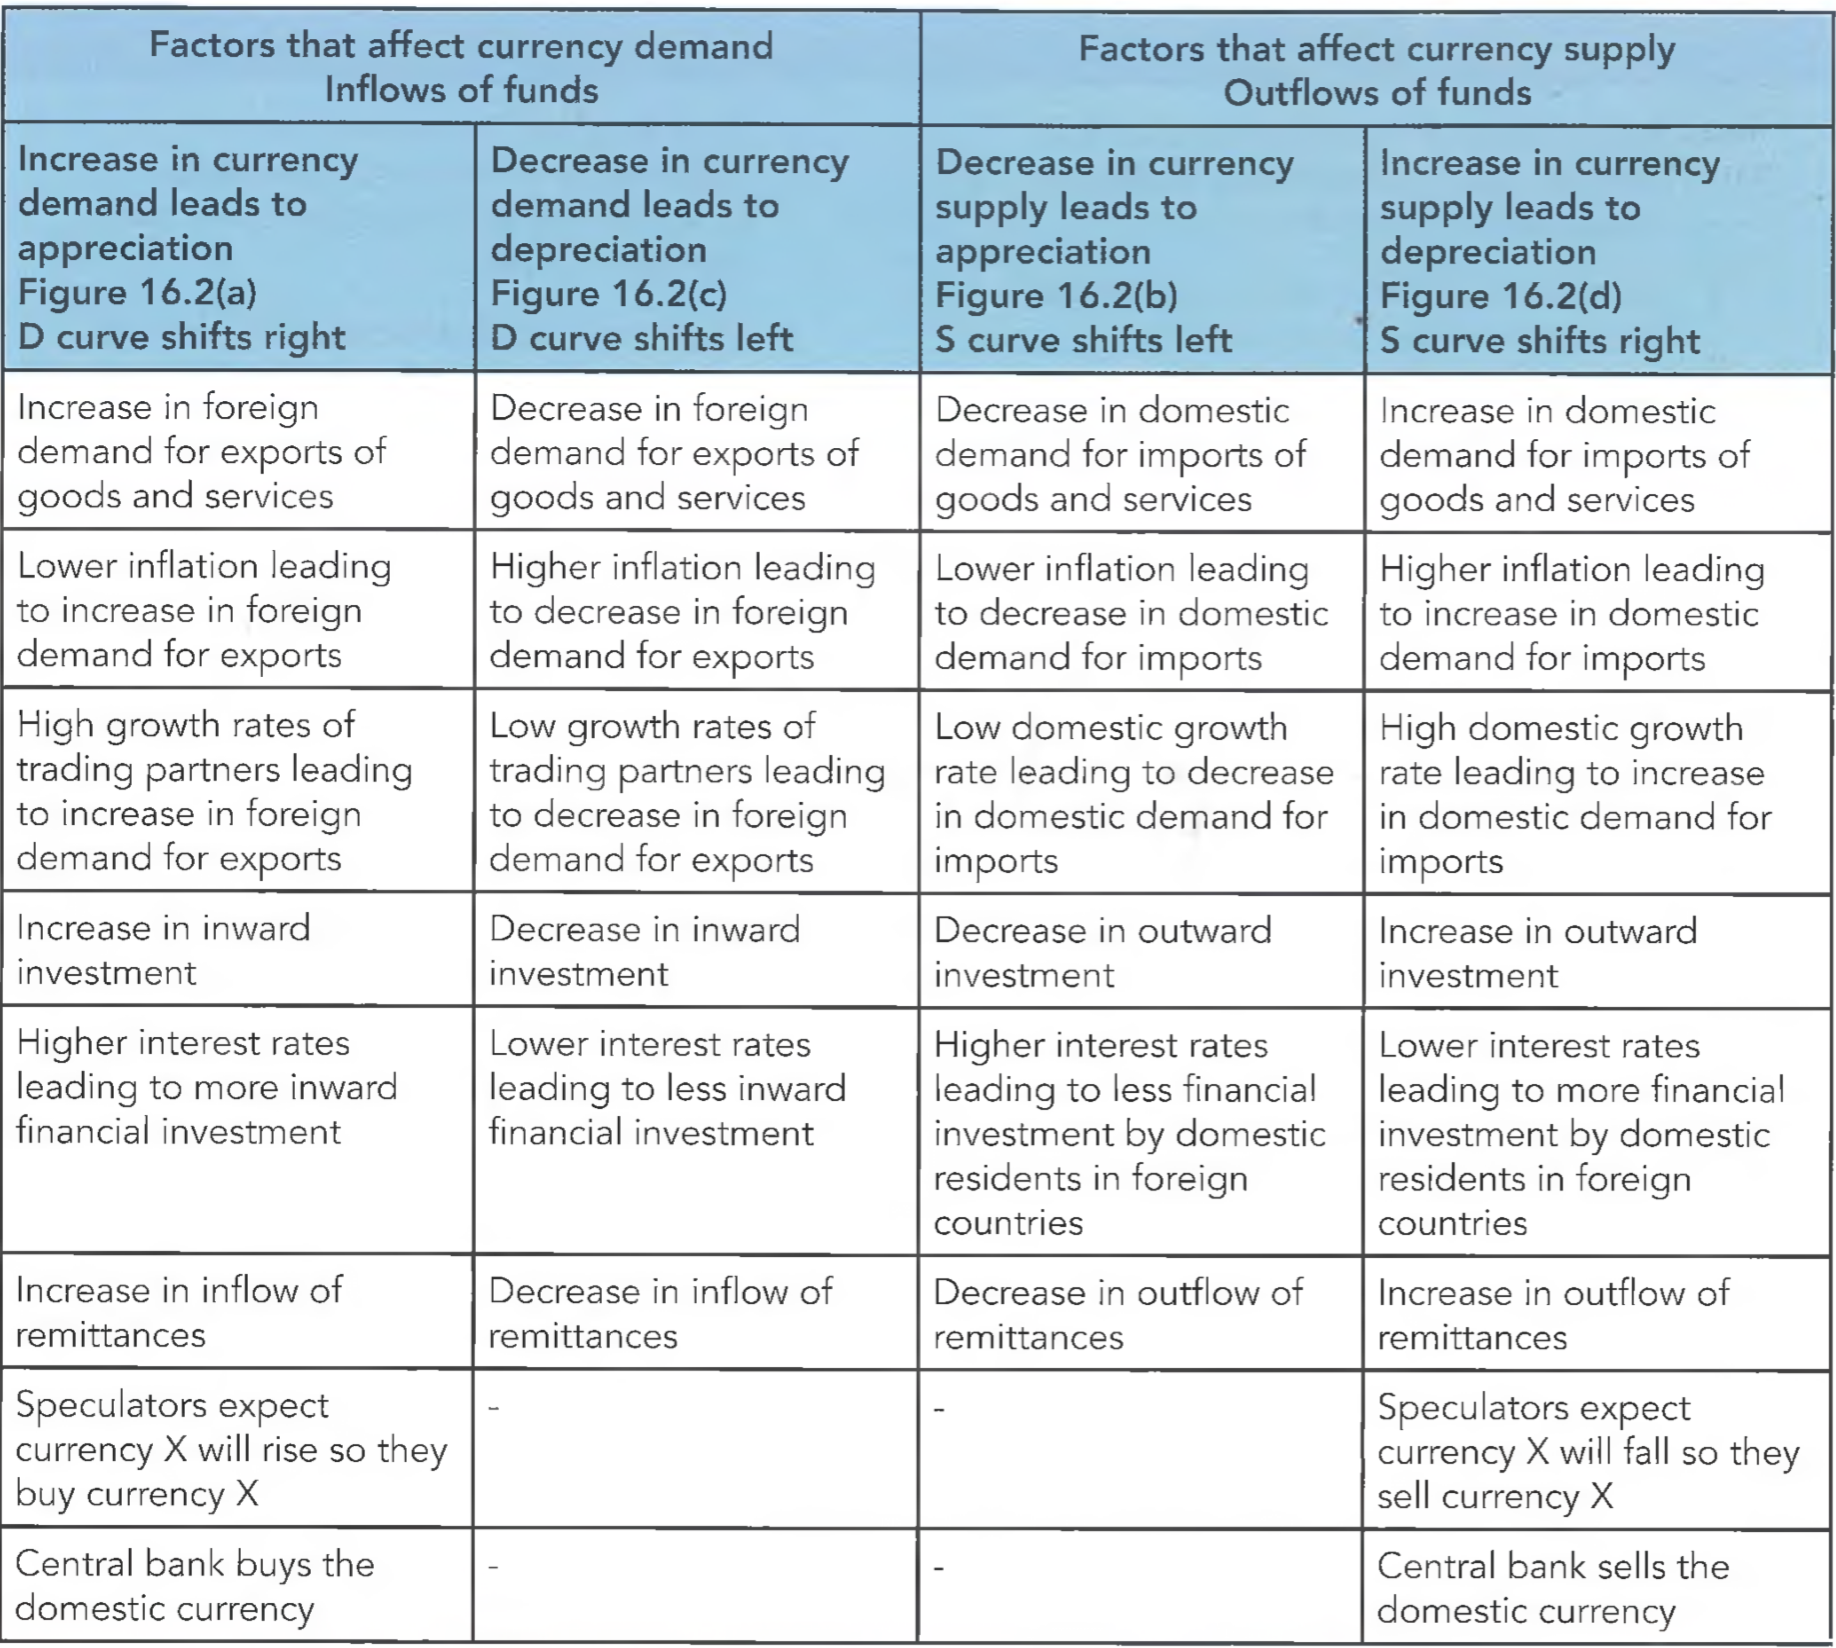
\includegraphics[width=0.9\linewidth]{Screenshot 2026-08-06 at 13.02.21.png}
\end{center}
\subsection{Consequences of changes in exchange rates: an evaluation}
When a currency appreciates, the following effects occur:
\begin{itemize}
  \item More foreign goods can be imported
  \item Foreigners can buy less of the domestic goods
  \item Combined, net exports will decrease
\end{itemize}
When a currency depreciates, the opposite effects occur.\\
\textbf{Depreciation effects}:
\begin{itemize}
  \item \textbf{Inflation}: (i) \textit{Demand-pull}: net exports ($X - M$) increase $\to$ AD shifts right $\to$ inflation if at/near potential output. (ii) \textit{Cost-push}: imported inputs become more expensive $\to$ SRAS shifts left $\to$ higher production costs $\to$ inflation.
  \item \textbf{Economic growth}: net exports increase $\to$ AD shifts right $\to$ \textbf{short-term growth} in real GDP. If export growth spurs investment $\to$ possible \textbf{long-term growth} (LRAS shifts right). \textit{However}, cost-push inflation (SRAS left) may reduce real GDP --- net effect depends on which is stronger.
  \item \textbf{Unemployment}: higher net exports $\to$ higher AD $\to$ lower \textbf{cyclical unemployment}; employment rises in export industries and import-competing industries. \textit{However}, cost-push inflation (SRAS left) may raise unemployment --- net effect depends on relative strength of AD increase vs.\ SRAS decrease.
  \item \textbf{Current account balance}: exports increase, imports decrease $\to$ trade \textbf{deficit shrinks} or surplus grows (HL: Marshall-Lerner condition, Chapter 17).
  \item \textbf{Foreign debt}: domestic currency buys less foreign currency $\to$ value of foreign debt \textbf{increases} (a major problem for developing countries).
  \item \textbf{Living standards}: imports more expensive $\to$ higher cost of living; cost-push + demand-pull inflation $\to$ lower real incomes; outbound travel more expensive. \textit{Unemployment effects mixed}.
\end{itemize}
\textbf{Appreciation effects}:
\begin{itemize}
  \item \textbf{Inflation}: net exports fall $\to$ AD decreases $\to$ \textbf{less demand-pull} inflation; cheaper imports $\to$ SRAS shifts right $\to$ \textbf{less cost-push} inflation.
  \item \textbf{Economic growth}: lower net exports $\to$ AD shifts left $\to$ \textbf{lower real GDP} growth.
  \item \textbf{Unemployment}: lower net exports $\to$ AD falls $\to$ \textbf{higher cyclical unemployment}; employment falls in export and import-competing industries.
  \item \textbf{Current account balance}: exports fall, imports rise $\to$ trade \textbf{deficit widens} or surplus shrinks.
  \item \textbf{Foreign debt}: domestic currency buys more foreign currency $\to$ value of foreign debt \textbf{decreases}.
  \item \textbf{Living standards}: cheaper imports $\to$ lower cost of living; lower inflation $\to$ higher real incomes; outbound travel cheaper. \textit{Unemployment effects mixed}.
\end{itemize}
\subsubsection*{Export industries vs import-competing industries}
\needbold{Export industries} are domestic industries that produce goods and services \textbf{sold to foreign buyers} (exported). \needbold{Import-competing industries} are domestic industries that produce goods and services \textbf{competing with imports} --- goods that domestic consumers could also buy from foreign producers. These two groups have \textbf{opposing interests} in exchange-rate and trade-policy changes:
\begin{itemize}
  \item \textbf{Effects of a currency depreciation}:
  \begin{itemize}
    \item \textbf{Export industries gain}: their goods become cheaper in foreign currency $\to$ exports rise $\to$ output, employment and profits in export industries increase (Tragakes: ``employment in export industries is likely to increase since exports are likely to rise'').
    \item \textbf{Import-competing industries gain}: imports become more expensive in domestic currency $\to$ consumers switch to domestic substitutes $\to$ sales, output and employment in import-competing industries rise (``employment in industries producing goods that compete with imports is also likely to increase since imports are expected to fall with depreciation'').
    \item \textbf{Import-dependent industries lose}: industries that rely heavily on imported inputs (e.g.\ electronics with imported components, automobiles using imported parts) face higher production costs, even though they may also compete with imports --- the cost-push effect may dominate.
  \end{itemize}
  \item \textbf{Effects of a currency appreciation}:
  \begin{itemize}
    \item \textbf{Export industries lose}: their goods become more expensive in foreign currency $\to$ exports fall $\to$ output, employment and profits fall.
    \item \textbf{Import-competing industries lose}: imports become cheaper $\to$ consumers switch to foreign goods $\to$ domestic sales and employment fall.
    \item \textbf{Import-dependent industries gain}: cheaper imported inputs lower production costs.
  \end{itemize}
  \item \textbf{Trade protection (tariffs, quotas)}: benefits \textbf{import-competing industries} (higher domestic price, larger quantity sold) but \textbf{harms export industries} indirectly --- protected inputs raise their costs, and trading partners may \textbf{retaliate} against the country's exports.
  \item \textbf{Trade liberalisation}: hurts \textbf{import-competing industries} (must now compete with lower-cost foreign producers; some firms close, workers lose jobs --- see the winners/losers discussion in Unit 4, \hyperref[sec:strategies]{Strategies to promote EG and ED}) while benefiting \textbf{export industries} (access to larger markets, cheaper imported inputs).
  \item \textbf{Policy significance}: the conflict between export and import-competing industries is central to exchange-rate policy (an undervalued currency favours both export and import-competing industries at the expense of consumers and import-dependent firms), trade-policy debates, and the politics of liberalisation.
\end{itemize}

\subsubsection*{Supplementary: International competitiveness (Edexcel Book 2 Ch 31)}
\needbold{International competitiveness} refers to the ability of a country's firms to sell their goods and services successfully in international and domestic markets against foreign competitors.
\begin{itemize}
  \item \textbf{Key indicators of competitiveness}:
  \begin{itemize}
    \item \textbf{Relative unit labour costs (RULC)}: total labour costs divided by real output, measured relative to trading partners. Lower RULC improves cost competitiveness.
    \item \textbf{Relative export prices}: export prices converted into a common currency relative to competitor nations.
    \item \textbf{Productivity}: labour productivity and total factor productivity; higher productivity offsets higher money wages.
    \item \textbf{Non-price factors}: product quality, reliability, brand reputation, customer service, innovation, and delivery speed.
  \end{itemize}
  \item \textbf{Policies to improve international competitiveness}:
  \begin{itemize}
    \item \textbf{Supply-side policies}: investment in human capital (education/training), modern infrastructure, tax incentives for R\&D, and reduction of regulatory burdens.
    \item \textbf{Exchange rate policy}: maintaining a competitive or depreciated exchange rate to keep export prices attractive in foreign markets.
    \item \textbf{Cost control}: wage restraint agreements and labour market flexibilities.
  \end{itemize}
\end{itemize}

\subsubsection*{Supplementary: Purchasing power parity (PPP) and exchange-rate calculations}
The \needbold{purchasing power parity (PPP) exchange rate} is the theoretical exchange rate at which an identical basket of goods and services costs exactly the same in two countries when expressed in the same currency:
\[\text{PPP exchange rate (local currency per foreign currency)} = \dfrac{\text{Price of basket in local currency}}{\text{Price of same basket in foreign currency}}\]
\begin{itemize}
  \item \textbf{Example}: suppose a representative basket of goods costs \textyen 12 in China and \$6 in the US:
  \[\text{PPP exchange rate} = \dfrac{\text{\textyen}12}{\$6} = \text{\textyen}2 \text{ per US\$}\]
  Under this PPP rate, an income of \textyen 12 in China provides the exact same purchasing power as \$6 in the United States.
  \item \needbold{PPP conversion factor}: the amount of domestic currency needed to purchase the equivalent volume of goods that US\$1 buys in the United States.
  \[\text{Value in PPP dollars} = \dfrac{\text{Local price}}{\text{PPP factor (local currency per US\$)}}\]
  \item \textbf{Unit-cancellation rule for calculations}:
  \begin{itemize}
    \item If the exchange rate is quoted in \textbf{local per foreign} currency (\textyen/\$): \textbf{divide} by the rate:
    \[\text{\textyen}12 \div (\text{\textyen}2 / \$1) = \$6\]
    \item If the exchange rate is quoted in \textbf{foreign per local} currency (\$/\textyen): \textbf{multiply} by the rate:
    \[\text{\textyen}12 \times (\$0.50 / \text{\textyen}1) = \$6\]
  \end{itemize}
  \item \textbf{Economic application}: PPP adjustments are essential when comparing GDP, GDP per capita, and living standards internationally because market exchange rates fail to account for large international differences in non-traded goods prices and domestic price levels. The \textbf{Big Mac Index} (compiled by \textit{The Economist}) is a popular simplified PPP illustration.
  \item \textbf{PPP vs.\ GDP Deflator}: do not confuse PPP with the GDP deflator. The GDP deflator ($= \frac{\text{Nominal GDP}}{\text{Real GDP}} \times 100$) measures domestic price inflation over time within an economy and involves no currency conversion.
  \item \textbf{Real exchange rate (RER)}:
  \[RER = e \times \dfrac{P_d}{P_f}\]
  where $e$ is the nominal exchange rate (foreign currency per unit of domestic currency), $P_d$ is the domestic price level, and $P_f$ is the foreign price level. A rise in RER indicates a real appreciation, eroding price competitiveness.
\end{itemize}

\subsection{Government intervention: fixed ER}
In a fixed exchange rate system, exchange rates are fixed by the central bank of each country at a particular level (or narrow range), and are not permitted to change freely in response to changes in currency supply and demand. The exchange rate is still determined by currency demand and supply, but these are manipulated by the central bank or government in order to arrive at the particular equilibrium that will give rise to the desired exchange rate. \\\\
This intervention takes the form of buying and selling reserve currencies by the central bank, as well as making other adjustments in the domestic economy.\\
\begin{center}
  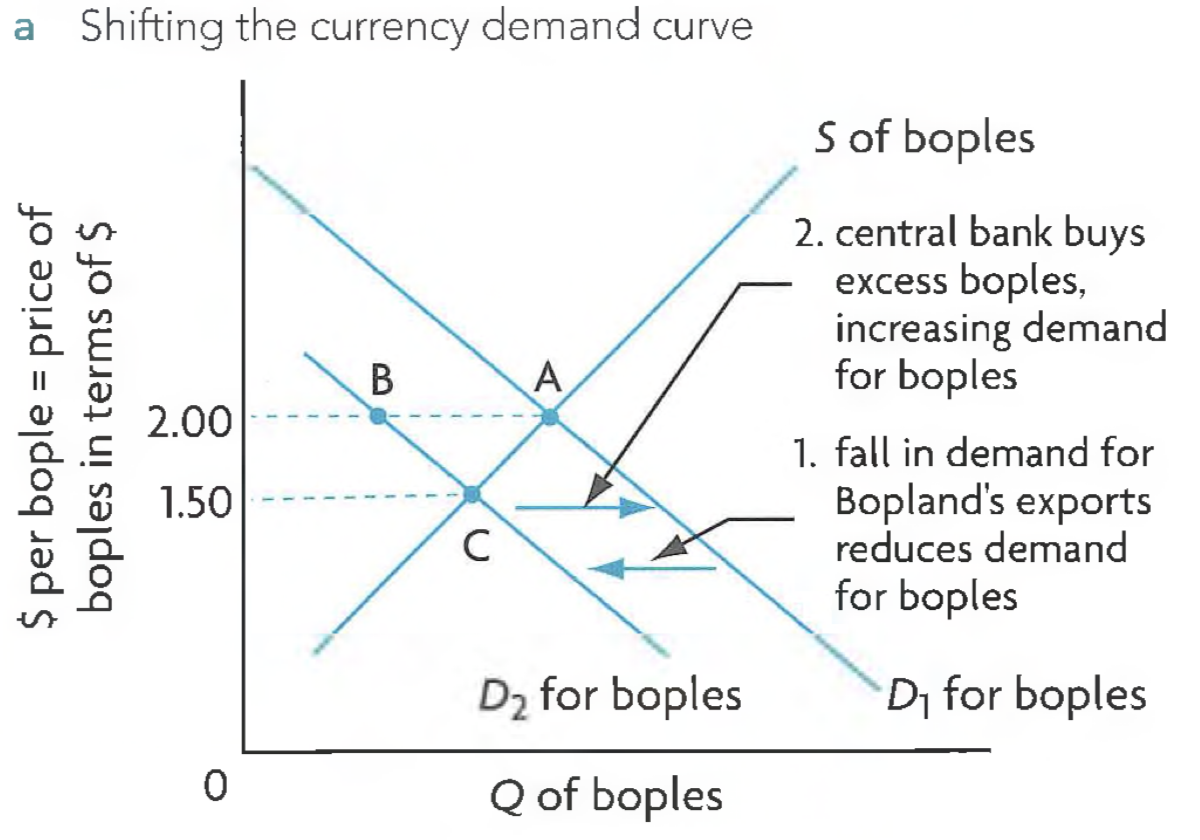
\includegraphics[width=0.45\linewidth]{Screenshot 2026-08-06 at 13.20.55.png}
  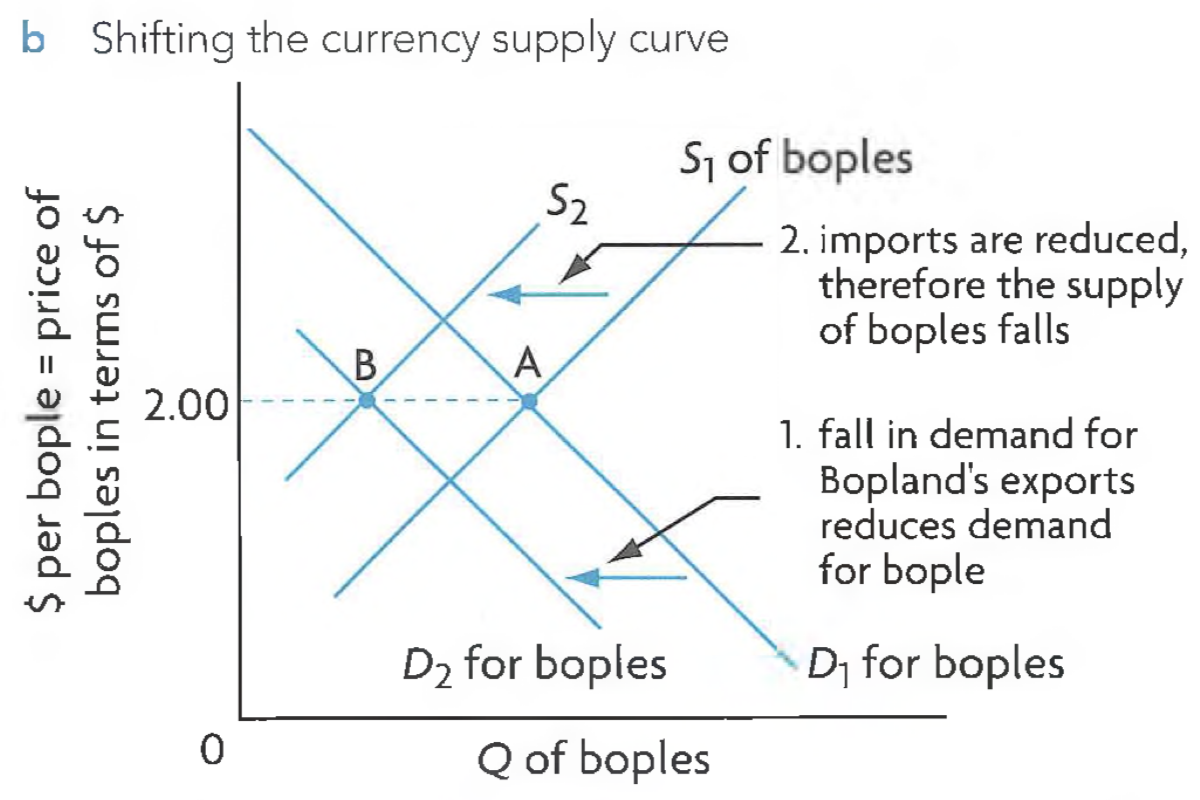
\includegraphics[width=0.45\linewidth]{Screenshot 2026-08-06 at 13.21.05.png}
\end{center}
\subsubsection*{Methods to maintain a fixed exchange rate}
\begin{enumerate}
  \item \textbf{Using official reserves}: the central bank buys excess domestic currency (sells foreign reserves) when there is excess supply, or sells domestic currency (buys foreign reserves) when there is excess demand. \textit{Limitation}: if excess supply persists, the central bank will eventually \textbf{run out of foreign reserves} and must use other methods.
  \item \textbf{Increasing interest rates}: attracts foreign financial investment $\to$ demand for domestic currency rises $\to$ maintains the fixed rate. \textit{Disadvantage}: contractionary monetary policy $\to$ may cause \textbf{recession}.
  \item \textbf{Borrowing from abroad}: foreign loans increase demand for domestic currency. \textit{Disadvantage}: accumulates \textbf{foreign debt} with associated costs (Chapters 19--20).
  \item \textbf{Efforts to limit imports}: reduces supply of domestic currency (less foreign exchange needed). Methods include: (a) contractionary fiscal/monetary policies $\to$ lower AD $\to$ lower incomes $\to$ fewer imports; (b) trade protection policies $\to$ directly reduce import quantities. \textit{Disadvantages}: contractionary policies may cause recession; trade protection invites retaliation $\to$ lower exports.
\end{enumerate}
\textit{Note}: if there is excess \textit{demand} for the currency (upward pressure), the central bank can keep selling domestic currency indefinitely (accumulating foreign reserves) --- reserves are not a constraint in this direction.
\begin{itemize}
  \item If the currency value is higher than what can be maintained through intervention, the government may change it to a new, lower value; this is called devaluation of the currency. (Like depreciation)
  \item If, on the other hand, the currency has a lower value than can be maintained by intervention, the government may set a new higher value; this is called revaluation. (Like appreciation)
\end{itemize}
\subsubsection*{Managed ER}
Combining elements of both, though closer to floating exchange rates, this is the current system. 
\begin{itemize}
  \item Exchange rates are for the most part free to float to their market levels over long periods of time.
  \item However, central banks periodically intervene to stabilise them over the short term. (prevent large and abrupt fluctuations in exchange rates that could arise if currencies were left entirely to market forces.)
\end{itemize}
Pegged ER: The pegged currency is allowed to fluctuate only within a narrow range above and below a target exchange rate relative to the dollar or the euro, so that if the actual exchange rate hits the upper or lower limit of the range, the central bank intervenes to keep it within the limits.\\\\
Overvalued currency: has a value that is too high relative to its equilibrium free market value. Its exchange rate has been set at a higher level than the equilibrium market exchange rate.\\
Undervalued currency: has a value that is too low relative to its equilibrium free market value. Its exchange rate is low relative to the one the market would have determined.\\
\textbf{Overvalued currencies}:
\begin{itemize}
  \item \textbf{Benefits}:
  \begin{itemize}
    \item \textbf{Cheaper imports}: capital goods, raw materials and other inputs become less expensive $\to$ speeds up \textbf{industrialisation} (main reason developing countries overvalue).
  \end{itemize}
  \item \textbf{Costs}:
  \begin{itemize}
    \item \textbf{Exports become more expensive} $\to$ hurts domestic exporters.
    \item \textbf{Worsening current account balance}: increased imports + reduced exports $\to$ payments difficulties.
    \item \textbf{Domestic producers hurt}: must compete with artificially cheap imports $\to$ negative effects on employment and resource allocation.
    \item Often forces eventual \textbf{devaluation} to correct the overvaluation.
  \end{itemize}
\end{itemize}
\textbf{Undervalued currencies}:
\begin{itemize}
  \item \textbf{Benefits}:
  \begin{itemize}
    \item \textbf{Exports become cheaper} to foreign buyers $\to$ expands export industries, economic growth and employment.
  \end{itemize}
  \item \textbf{Costs}:
  \begin{itemize}
    \item \textbf{Imports become more expensive} $\to$ possible \textbf{cost-push inflation}.
    \item Considered an \textbf{unfair competitive advantage} (``cheating'') $\to$ harms trading partners who face increased imports and lower exports.
    \item In a managed float, this is called a \textbf{``dirty float''}.
    \item Correction requires \textbf{revaluation} (appreciation) of the currency.
  \end{itemize}
\end{itemize}
\subsection{The balance of payments}
The \needbold{balance of payments} of a country is a record (usually for a year) of all transactions between the residents of the country and the residents of all other countries. Its role is to show all payments received from other countries, called credits, and all payments made to other countries, called debits. In the course of a year, all inflows of payments (credits) must exactly equal the outflows of payments (debits); the sum of all credits is equal to the sum of all debits.
\begin{itemize}
  \item All credits (inflows of money into the country) create a foreign demand for the country's currency;
  \item All debits (outflows of money from the country) create a supply of the domestic currency.
\end{itemize}
\begin{center}
  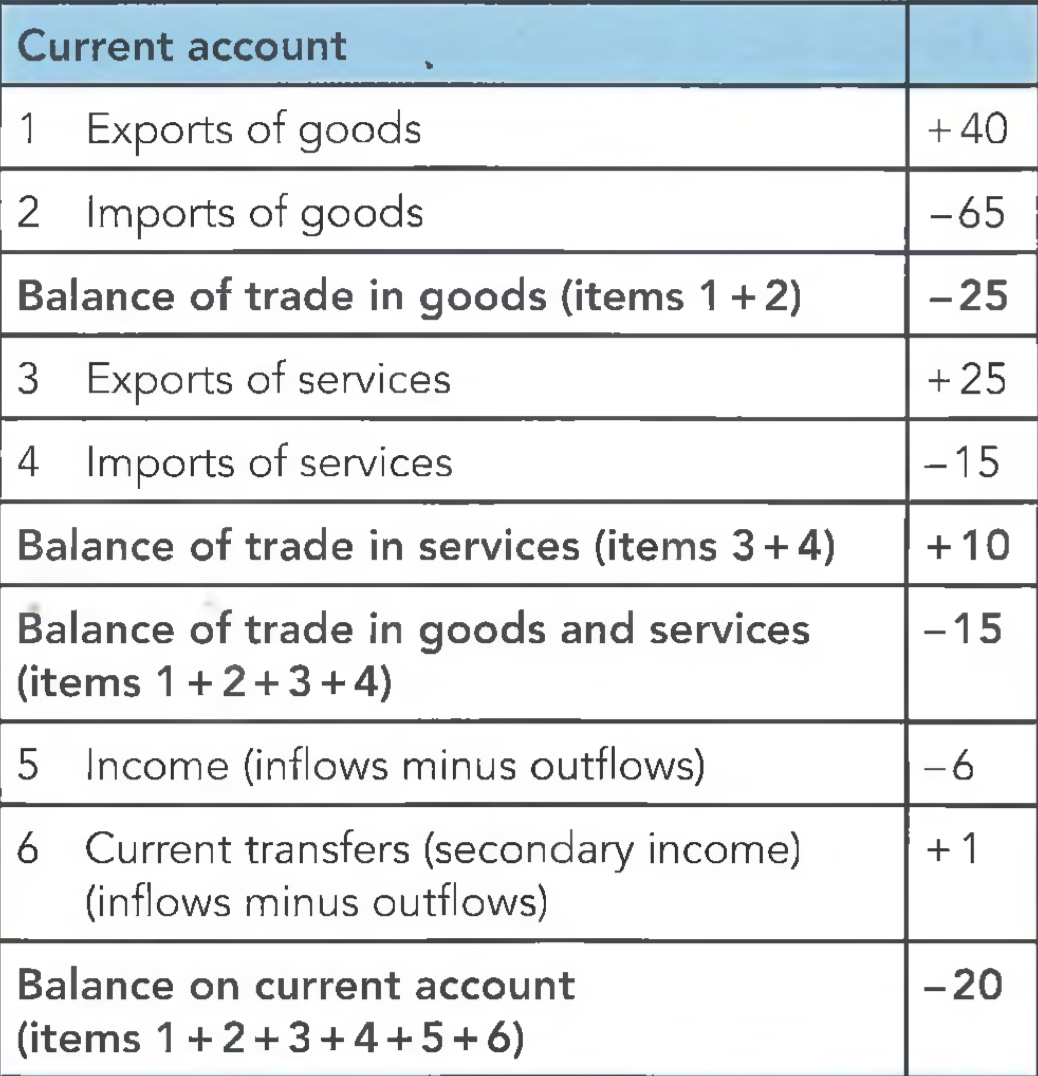
\includegraphics[width=0.36\linewidth]{Screenshot 2026-08-06 at 13.46.35.png}
  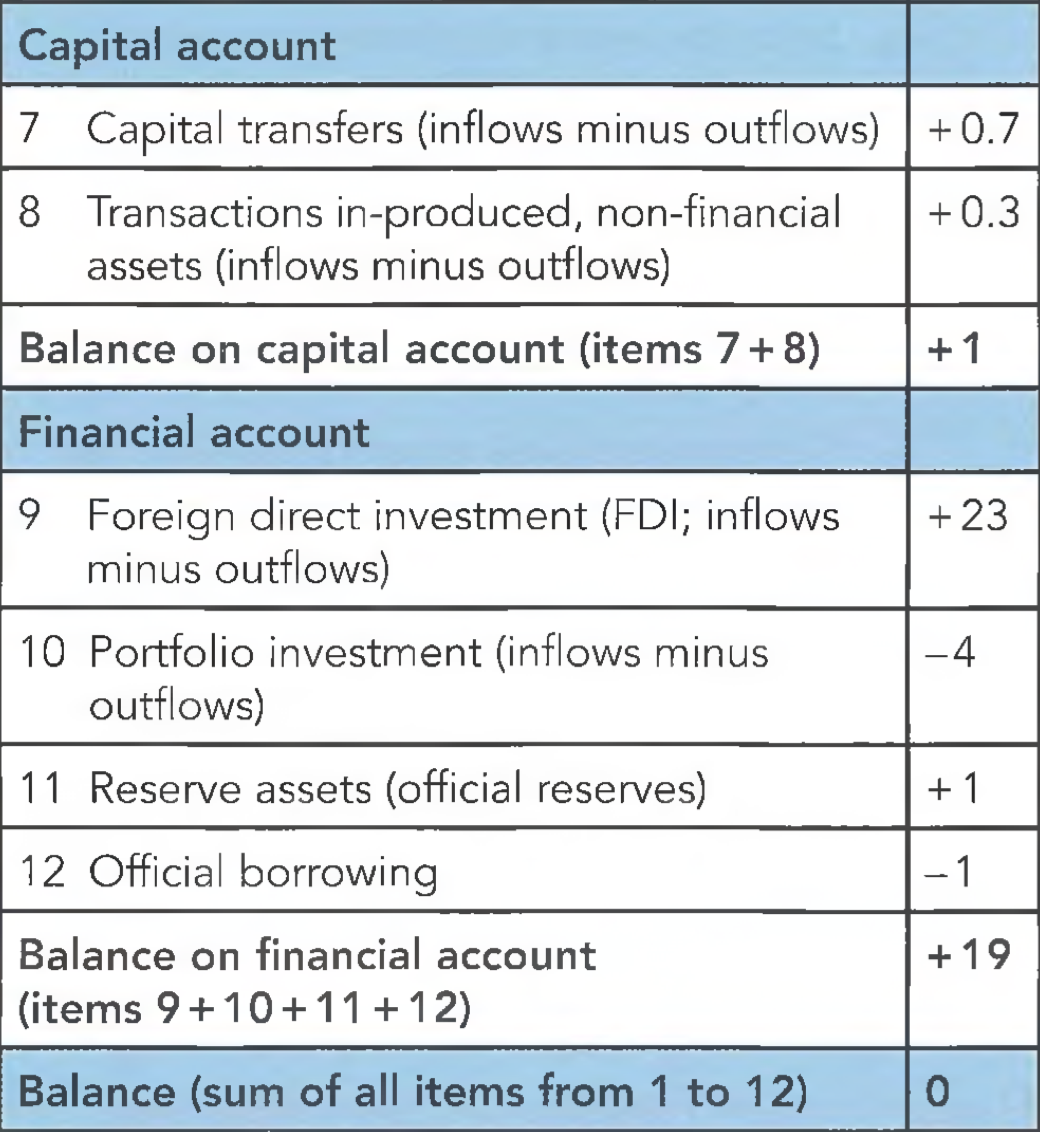
\includegraphics[width=0.35\linewidth]{Screenshot 2026-08-06 at 13.46.49.png}
\end{center}
A surplus in an account occurs whenever a balance has a positive value, meaning that credits are larger than debits (there is an excess of credits).\\
A deficit in an account occurs whenever a balance has a negative value, meaning that debits are larger than credits (there is an excess of debits).
\subsubsection*{The current account}
\begin{enumerate}
  \item \textbf{Balance of trade in goods}: exports of goods (credit, $+$) minus imports of goods (debit, $-$). A negative balance = \textbf{deficit} in goods trade.
  \item \textbf{Balance of trade in services}: exports of services (credit, $+$) minus imports of services (debit, $-$). Services include insurance, tourism, transportation, consulting. Foreign tourists visiting = export of tourism services; domestic tourists going abroad = import of tourism services.
  \item \textbf{Balance of trade in goods and services} (``trade balance'' / ``net exports'' $X - M$): sum of items 1--4.
  \item \textbf{Income}: inflows of rents, interest, profits and dividends from abroad (credit) minus outflows (debit). Includes income from rental property, bank accounts, stocks, and subsidiary profits abroad.
  \item \textbf{Current transfers}: inflows of gifts, remittances (money sent home by workers abroad), foreign aid, pensions (credit) minus outflows (debit).
\end{enumerate}
\subsubsection*{The capital account}
The capital account consists of two items:
\begin{itemize}
  \item \textbf{Capital transfers}: inflows minus outflows for debt forgiveness (cancelled debt), non-life insurance claims, and investment grants (gifts from governments to finance physical capital).
  \item \textbf{Transactions in non-produced, non-financial assets}: purchase/use of natural resources not produced (land, mineral rights, forestry rights, water, fishing rights, airspace, electromagnetic spectrum). Inflows (credits) minus outflows (debits).
\end{itemize}
\textbf{Capital account balance} $=$ sum of both items. A surplus means credits $>$ debits $\to$ excess demand for the domestic currency in the forex market.
\subsubsection*{The financial account}
The financial account consists of four items:
\begin{itemize}
  \item \textbf{Foreign direct investment (FDI)}: inward investment by foreign multinational corporations in productive facilities (buildings, factories) --- credits; minus outward investment by domestic firms abroad --- debits.
  \item \textbf{Portfolio investment}: inflows for purchase of domestic stocks/bonds by foreigners (credits) minus outflows for purchase of foreign stocks/bonds by domestic residents (debits).
  \item \textbf{Reserve assets}: foreign currency reserves bought/sold by the central bank to influence the exchange rate. Selling foreign currency (buying domestic currency) $=$ credit; buying foreign currency (selling domestic currency) $=$ debit.
  \item \textbf{Official borrowing}: government borrowing from abroad (credits) minus loans to foreign governments (debits).
\end{itemize}
\textbf{Financial account balance} $=$ sum of all four items. A surplus means credits $>$ debits $\to$ excess demand for the domestic currency.\\\\
\textit{Note}: the \textbf{current account} and \textbf{financial account} are linked --- a current account deficit must be financed by an equal surplus in the financial account (capital inflows, reserve sales, or borrowing). The two accounts (plus the capital account and statistical discrepancy) sum to zero.
\subsubsection*{Why is there a zero balance in BoP?}
Recall that:
\begin{enumerate}
  \item All credits in the balance of payments create demand for a currency, and all debits create supply of the currency.
  \item ER are always determined by currency demand and supply, in both floating and fixed exchange rate systems.
\end{enumerate}
It follows then that at the point where an equilibrium exchange rate is determined, in other words at the point where currency demand equals currency supply, it is also the case that the sum of credits is equal to the sum of debits. Therefore deficits must match surpluses.
\subsubsection*{Why are current and financial account interdependent?}
\begin{itemize}
  \item \textbf{Current account deficit} ($M > X$): the country \textbf{consumes more than it produces} --- consuming at a point \textbf{outside its PPC}. The excess imports must be paid for $\to$ \textbf{financial account surplus} (foreigners invest/lend to the country, providing the needed foreign exchange). The deficit is \textit{financed} by borrowing from abroad.
  \item \textbf{Current account surplus} ($X > M$): the country \textbf{produces more than it consumes} --- consuming at a point \textbf{inside its PPC}. The excess foreign exchange earned from exports is used to \textbf{buy assets abroad} (FDI, portfolio investment, loans) $\to$ \textbf{financial account deficit}.
\end{itemize}
Most economists believe the financial account balance is often a \textbf{reflection} of what is happening in the current account: a financial account surplus exists to finance the current account deficit (or vice versa).\\
\textit{(Note: consuming outside the PPC via a trade deficit is very different from achieving this via comparative advantage. Comparative advantage assumes $X = M$ --- the gain comes from \textbf{allocative efficiency}. A trade deficit is temporary and creates debt liabilities; comparative advantage gains are sustainable.)}\\\\
BoP deficit: deficit in the combined accounts \emph{excluding central bank intervention}\\
BoP surplus: surplus in the combined accounts \emph{excluding central bank intervention}
\section{Further topics on exchange rates and the balance of payments}
\subsection{How the current account and the financial account are related to ER}
Under floating exchange rates, when there is a deficit in the current account, market forces create a downward pressure on the currency exchange rate. When there is a surplus in the current account, market forces create an upward pressure on the currency exchange rate. As a result, exchange rate changes automatically eliminate current account deficits and surpluses (by the change in ER that causes net export to change), and create a balance in the balance of payments.\\\\
The most common intervention (of ER) involves buying and selling of reserve currencies (reserve assets). \\\\
How to increase credits:
\begin{itemize}
  \item Increase IR, attracting FDI
  \item Borrow from abroad
\end{itemize}
How to decrease debits:
\begin{itemize}
  \item Limit imports (through contractionary fiscal and monetary policies or trade protection)
  \item Impose exchange controls (limits to the amount of domestic currency that can be exchanged for foreign currencies)
\end{itemize}
In a fixed exchange rate system, the balance of payments are made to balance by policies that change currency demand or supply in order to keep the exchange rate fixed.\\
Everything that is recorded in the balance of payments creates a demand for or supply of a domestic currency.\\\\
The financial account can exert an influence on ER. While the financial account is partly a reflection of the current account, it can also \textbf{independently affect the exchange rate}:
\begin{itemize}
  \item \textbf{Financial account surplus $\to$ appreciation}: if higher domestic interest rates attract capital inflows, credits in the financial account increase (more foreign demand for domestic currency). Simultaneously, domestic investors keep funds at home $\to$ fewer debits. More credits $+$ fewer debits $=$ excess demand for currency $\to$ \textbf{appreciation} (even if the current account deficit is unchanged).
  \item \textbf{Financial account deficit $\to$ depreciation}: if capital flows out (e.g.\ lower domestic interest rates, or speculation of depreciation), debits exceed credits $\to$ excess supply of currency $\to$ \textbf{depreciation}.
  \item \textbf{Capital flight}: if speculators expect sharp depreciation, massive outflows can cause \textbf{very large depreciation} (a self-fulfilling crisis; see Chapter 19).
\end{itemize}
\subsubsection*{Fiscal and monetary policy in an open economy (supplementary)}
\textbf{Fiscal policy}: an \textbf{expansionary} fiscal policy financed by government borrowing tends to \textbf{raise interest rates}, which (i) \textbf{crowds out} private investment and (ii) in an open economy \textbf{appreciates the currency} $\to$ exports fall and imports rise ($X - M$ falls) $\to$ both effects weaken the expansionary impact of the spending increase.
\textbf{Monetary policy}:
\begin{itemize}
  \item \textbf{Expansionary} monetary policy (lower interest rates) \textbf{depreciates} the currency $\to$ exports rise and imports fall ($X - M$ rises) $\to$ this \textbf{strengthens} the expansionary effect. Effect on the trade balance: a trade \textbf{deficit shrinks}, a trade \textbf{surplus grows}.
  \item \textbf{Contractionary} monetary policy (higher interest rates) \textbf{appreciates} the currency $\to$ $X - M$ falls $\to$ this \textbf{strengthens} the contractionary effect. Effect on the trade balance: a trade \textbf{deficit grows}, a trade \textbf{surplus shrinks}.
\end{itemize}
\textbf{Special cases}:
\begin{itemize}
  \item \textbf{Defending the currency against speculation}: raising interest rates makes the currency more attractive, but may cause (or deepen) a \textbf{recession}.
  \item \textbf{Cost-push inflation from higher import prices}: higher interest rates appreciate the currency and lower import prices (helping correct cost-push inflation), but risk a recession --- and the economy may already be in recession from the negative SRAS shift.
\end{itemize}
Under \textbf{fixed} exchange rates, fiscal and monetary policy must respond to balance-of-payments needs; under \textbf{floating} rates, they can target domestic goals, but may have unintended foreign-sector consequences.

\subsection{Comparing and contrasting exchange rate systems}

\begin{center}
\renewcommand{\arraystretch}{1.4}
\footnotesize
\begin{tabular}{p{0.2\linewidth}|p{0.36\linewidth}|p{0.36\linewidth}}
\toprule
\textbf{Criterion} & \textbf{Fixed exchange rates} & \textbf{Floating exchange rates} \\
\midrule
\textbf{Exchange rate determination} & Set by the central bank at a particular level; not permitted to change freely. & Determined by market forces (demand and supply); no central bank intervention. \\
\textbf{Uncertainty \& stability} & \textbf{Stable} --- exchange rate does not change $\to$ certainty for trade and investment $\to$ better resource allocation and more international trade. & \textbf{Uncertain} --- future exchange rate unknown $\to$ negative effects on trade, investment planning; large/abrupt changes can cause financial crises. \\
\textbf{Foreign currency reserves} & Central bank must hold \textbf{sufficient reserves} to intervene (buy/sell currency). Problems arise if reserves run out. & \textbf{No need} for reserves --- balance of payments balances through market forces. \\
\textbf{Correction of current account imbalances} & \textbf{No easy method} --- cannot use exchange rate changes; must use contractionary policies (interest rate hikes, borrowing, import limits, trade protection) $\to$ may cause recession, debt, inefficiency. & \textbf{Automatic correction} --- deficit $\to$ depreciation $\to$ exports cheaper, imports more expensive $\to$ deficit shrinks (if Marshall-Lerner condition holds). \\
\textbf{Policy flexibility} & \textbf{No flexibility} --- must pursue policies to maintain the fixed rate (higher interest rates, borrowing, contractionary fiscal/monetary, trade protection) $\to$ may cause recession, debt, retaliation. & \textbf{High flexibility} --- policy can focus on domestic priorities (growth, employment); current account corrects itself via depreciation/appreciation. \\
\textbf{Inflation} & Fixed rates provide \textbf{anti-inflationary discipline} --- the need to maintain the rate forces contractionary policies when currency is under downward pressure. & \textbf{Less discipline} --- governments can pursue expansionary policies $\to$ inflation may result; depreciation can also cause imported inflation. \\
\textbf{Speculation} & \textbf{Limited} --- rate cannot move (exception: speculation about devaluation/revaluation). & \textbf{Unlimited} --- speculators can cause large exchange rate movements; risk of capital flight and self-fulfilling crises. \\
\textbf{Monetary policy independence} & \textbf{Lost} --- must use interest rates to maintain the exchange rate, not for domestic objectives. & \textbf{Retained} --- interest rates can be set for domestic goals (inflation, growth, unemployment). \\
\textbf{Trade \& investment} & \textbf{Favoured} --- stability encourages trade and investment flows; accurate price calculations across countries. & \textbf{Discouraged} --- uncertainty hampers trade/investment planning; volatile rates complicate international transactions. \\
\bottomrule
\end{tabular}
\end{center}
\subsection{Evaluating monetary union}
\needbold{Monetary union} $=$ common market $+$ \textbf{common currency} $+$ \textbf{common central bank}. Like a permanently fixed exchange rate system among members, with no possibility of devaluation/revaluation (e.g.\ European Monetary Union / euro zone).
\\
\textbf{Advantages}:
\begin{itemize}
  \item \textbf{Eliminates exchange rate risk and uncertainty} $\to$ benefits importers, exporters, consumers, investors $\to$ encourages trade and investment $\to$ more efficient resource allocation.
  \item \textbf{Encourages price transparency}: prices in a single currency are directly comparable across member countries $\to$ greater competition, lower prices, better consumer choice.
  \item \textbf{Lower transaction costs}: no need to exchange currencies $\to$ cost savings for businesses and travellers.
  \item \textbf{Lower interest rates} (for historically high-inflation countries): the common central bank's credibility anchors inflation expectations $\to$ lower risk premiums $\to$ cheaper borrowing.
  \item \textbf{Greater FDI inflows}: stable currency, larger market, no exchange risk attract foreign investment.
  \item \textbf{Political integration benefits}: fosters closer political co-operation, sense of shared identity.
\end{itemize}
\textbf{Disadvantages}:
\begin{itemize}
  \item \textbf{Loss of independent monetary policy}: the single central bank sets one interest rate for all members (``one-size-fits-all'') $\to$ cannot address country-specific conditions (different inflation, unemployment, growth rates). The ECB's policy may suit Germany but not Greece.
  \item \textbf{Loss of exchange rate as an adjustment mechanism}: a member with a trade deficit cannot depreciate/devalue to restore competitiveness $\to$ must rely on painful contractionary fiscal policy (spending cuts, tax increases) $\to$ recession, unemployment, social costs (Greek crisis, 2010--18).
  \item \textbf{Fiscal policy constraints}: convergence requirements limit budget deficits ($\leq 3\%$ of GDP) and public debt ($\leq 60\%$ of GDP) $\to$ reduces policy flexibility during recessions.
  \item \textbf{Risk of asymmetric shocks}: if a recession hits one member but not others, the affected country cannot use monetary or exchange rate policy to respond $\to$ deep, prolonged recessions.
  \item \textbf{No lender of last resort}: individual member central banks cannot print money to bail out domestic banks $\to$ financial instability risk.
  \item \textbf{Unequal distribution of costs and benefits}: stronger economies (e.g.\ Germany) benefit from an ``undervalued'' currency $\to$ large trade surpluses; weaker economies lose competitiveness and accumulate debt. Calls for a common fiscal authority to transfer funds to depressed regions face political opposition.
\end{itemize}
\subsection{Understanding current account deficits and surpluses}
\subsubsection*{Consequences of persistent current account deficits}
A current account deficit allows a country to consume more than it produces (outside its PPC), but this \textbf{cannot continue indefinitely}. Persistent deficits lead to:
\begin{itemize}
  \item \textbf{Foreign debt accumulation}: financed by financial account surpluses (borrowing from abroad, selling assets) $\to$ debt grows over time.
  \item \textbf{Declining confidence \& credit ratings}: international agencies downgrade creditworthiness $\to$ harder to borrow; must offer higher interest rates $\to$ deepens recession.
  \item \textbf{Asset sales}: country may be forced to sell domestic physical/financial assets to foreigners $\to$ loss of domestic ownership.
  \item \textbf{Import shortages}: if foreign exchange runs low, country may be unable to secure essential imports (oil, capital goods, inputs for production).
  \item \textbf{Painful demand management}: contractionary monetary/fiscal policies needed to reduce imports $\to$ lower incomes, recession, unemployment.
  \item \textbf{Lower economic growth}: accumulating debt + contractionary policies + declining confidence $\to$ lower long-term growth.
  \item \textbf{Currency depreciation pressure}: excess supply of domestic currency in the forex market $\to$ downward pressure; if investors panic, sharp depreciation or capital flight.
\end{itemize}
\subsubsection*{Methods to correct persistent current account deficits}
\textbf{1. Expenditure-switching policies} (switch spending from imports to domestic goods):
\begin{itemize}
  \item \textbf{Depreciation/devaluation}: makes exports cheaper and imports more expensive $\to$ switches consumption toward domestic goods. \textit{Risks}: cost-push inflation (higher import prices); may worsen deficit initially if PEDs are low (J-curve effect); requires Marshall-Lerner condition ($PED_m + PED_x > 1$).
  \item \textbf{Trade protection} (tariffs, quotas): directly restricts imports. \textit{Risks}: inefficiency, higher prices, resource misallocation, retaliation $\to$ lower exports.
\end{itemize}
\textbf{2. Expenditure-reducing policies} (reduce overall spending $\to$ fewer imports):
\begin{itemize}
  \item \textbf{Contractionary monetary policy}: higher interest rates $\to$ lower $C$ and $I$ $\to$ lower incomes $\to$ fewer imports. \textit{Risks}: recession, unemployment.
  \item \textbf{Contractionary fiscal policy}: lower $G$ / higher taxes $\to$ lower AD $\to$ lower incomes $\to$ fewer imports. \textit{Risks}: recession, unemployment.
\end{itemize}
\textbf{3. Supply-side policies} (improve competitiveness, long-term):
\begin{itemize}
  \item Market-based policies (lower costs, increase efficiency) $\to$ SRAS and LRAS shift right $\to$ lower inflation, more competitive exports, higher potential output.
  \item Interventionist policies (education, training, infrastructure, R\&D) $\to$ higher productivity, better export quality, reduced structural unemployment.
  \item \textit{Advantage}: no negative short-term demand effects. \textit{Disadvantage}: long time lags.
\end{itemize}
\subsubsection*{Consequences of persistent current account surpluses}
Countries with persistent surpluses produce more than they consume (consuming \textit{inside} their PPC) and are net lenders/asset buyers abroad (financial account deficit). Consequences:
\begin{itemize}
  \item \textbf{Low domestic consumption and living standards}: production exceeds consumption $\to$ lower standards of living than potentially achievable.
  \item \textbf{Insufficient domestic investment}: funds flow abroad (financial account deficit) $\to$ risk of underinvestment domestically $\to$ limited growth prospects.
  \item \textbf{Currency appreciation pressure}: surplus $\to$ upward pressure on exchange rate $\to$ exports become more expensive, imports cheaper $\to$ net exports may fall $\to$ lower AD.
  \item \textbf{Lower inflation}: reduced net exports $\to$ lower demand-pull inflation; cheaper imports $\to$ lower cost-push inflation.
  \item \textbf{Mixed employment effects}: lower AD may raise unemployment; but firms benefiting from cheaper imports may hire more.
  \item \textbf{Reduced export competitiveness}: appreciation makes exports dearer to foreigners $\to$ harder to compete globally.
  \item \textbf{Risk of retaliation}: persistent surpluses correspond to deficits in trading partners $\to$ deficit countries may impose trade barriers against surplus countries.
\end{itemize}
\subsubsection*{Marshall-Lerner condition and J-curve}
When a country's currency devalues or depreciates, its imports become more expensive domestically and exports become less expensive to foreigners.\\
The Marshall-Lerner condition is a condition that, if satisfied, allows devaluation or depreciation to lead to an improvement in a country's balance of trade (and therefore in its current account). Involves the PED for imports and exports (from domestic and foreign consumers).
\begin{itemize}
  \item If $PED_m<1$, a percentage increase in the price of imports (due to the devaluation/depreciation) leads to a smaller percentage decrease in quantity of imports demanded (inelastic) so that the value of imports increases, producing a negative effect on the trade balance.
  \item If $PED_m>1$, the value of imports will fall, producing a positive effect on the trade balance.
  \item (The larger the $PED_x$, the larger the increase in quantity of exports that results following a devaluation/depreciation, and the larger the positive effect on the trade balance.)
\end{itemize}
A better, formal statement of Marshall-Lerner condition:
\begin{itemize}
  \item If the sum of the PEDs for imports and exports is greater than 1, i.e. PEDm + PEDx >1, devaluation/depreciation will improve the trade balance (will make a trade deficit smaller).
  \item If the sum of the two PEDs is less than 1, devaluation/depreciation will worsen the trade balance (will make a trade deficit bigger).
  \item If the sum of the two PEDs is equal to 1, devaluation/depreciation will leave the trade balance unchanged.
\end{itemize}
J-curve effect: shown in a graph that plots the balance of trade (the value of exports minus imports) on the vertical axis and time on the horizontal axis. 
\begin{enumerate}
  \item A devaluing/depreciating country may see a worsening trade balance in the period immediately following the devaluation or depreciation of its currency;
  \item Later, the trade deficit will begin to shrink, and the trade balance will begin to improve.
\end{enumerate}
\begin{center}
  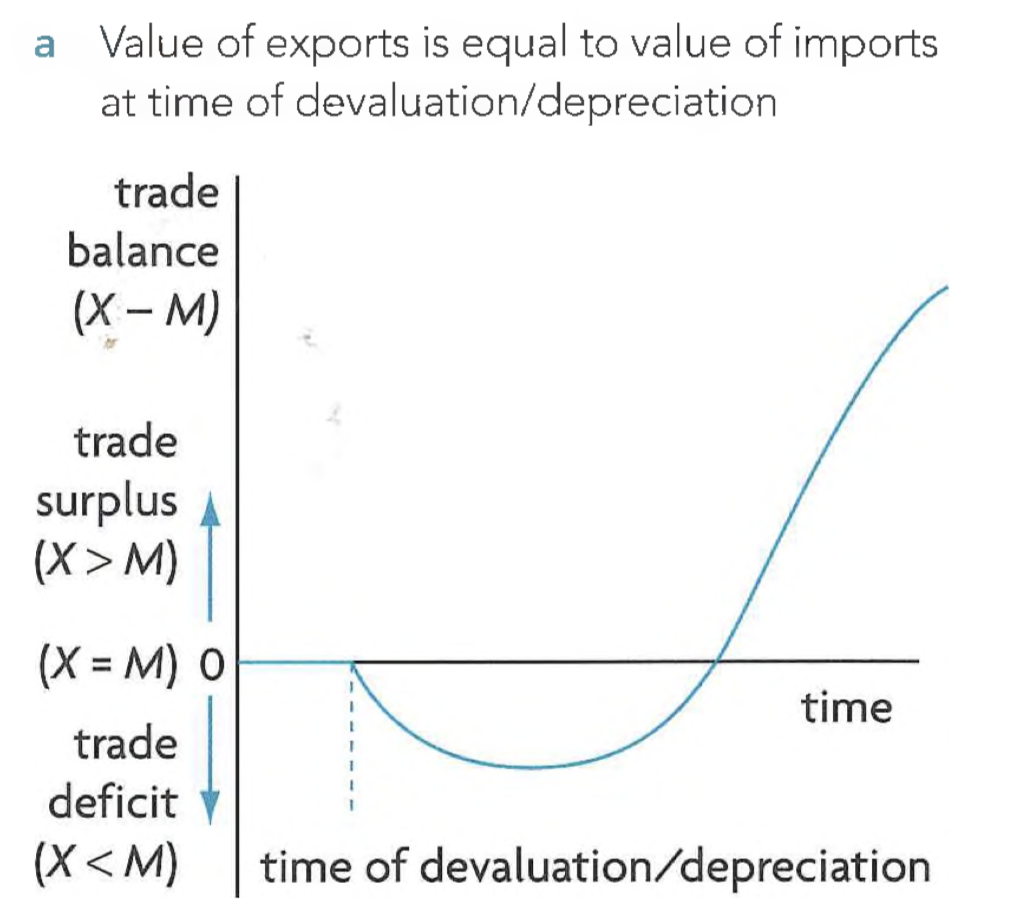
\includegraphics[width=0.4\linewidth]{Screenshot 2026-08-08 at 15.04.18.png}
  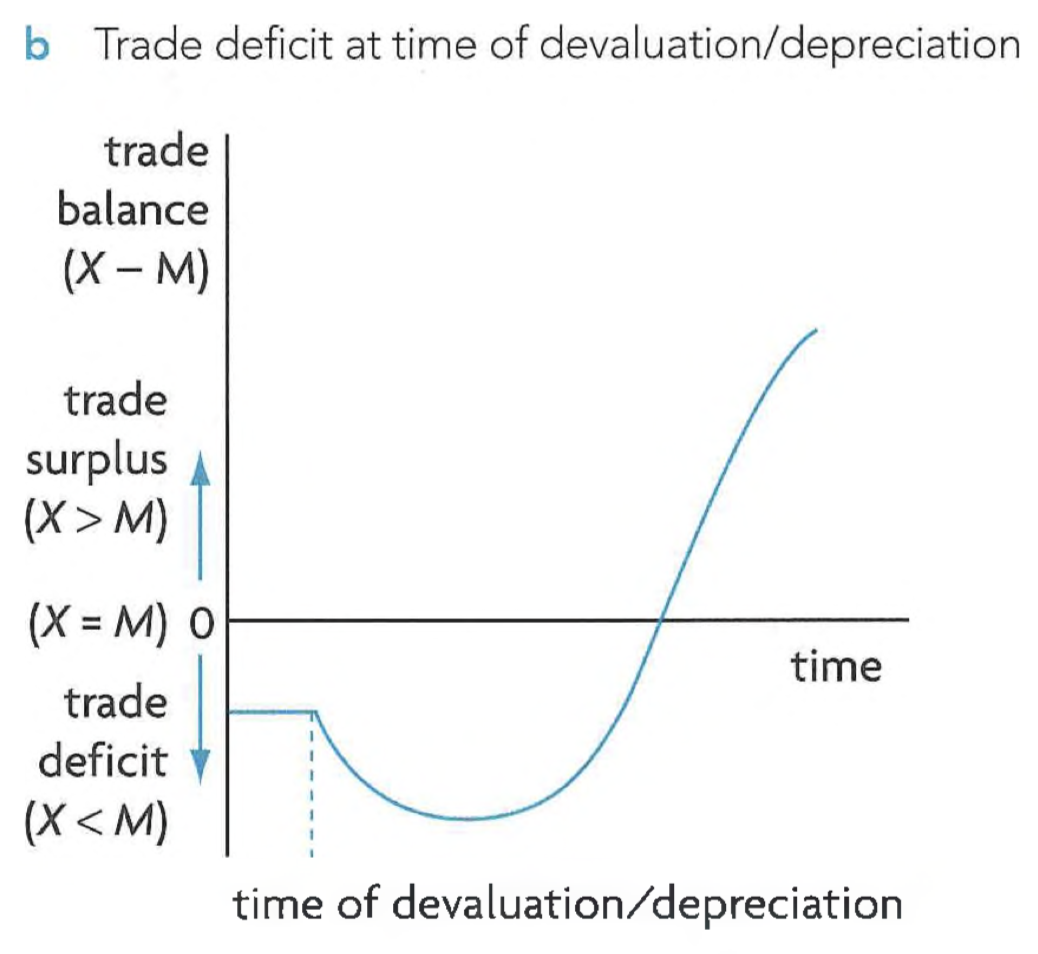
\includegraphics[width=0.4\linewidth]{Screenshot 2026-08-08 at 15.04.32.png}
\end{center}
The explanation behind the shape of the J-curve can be traced directly to the Marshall-Lerner condition. 
\begin{itemize}
  \item In the period immediately following a currency devaluation / depreciation, price elasticities of demand for imports and exports are very low, and the Marshall-Lerner condition is not satisfied: PEDm + PEDX < 1. Therefore the trade balance deteriorates. (Caused by time lags / delays. Consumers / producers need time to adjust to the new prices / affected by prior commitments.)
  \item As time passes, PEDs for imports and exports increase, and if there comes a point when PEDm + PEDx > 1, the trade balance begins to improve.
\end{itemize}
\section{Understanding economic development}\label{sec:development}
\subsection{Sustainable development}
The problem of sustainability arises because of conflicts between environmental and economic goals.\\
Recall that \needbold{sustainable development} is defined as development that meets the needs of the present without compromising the ability of future generations to meet their own needs.\\
It means that societies should pursue economic growth that does not deplete or degrade natural resources, so that future generations will not have fewer or lower-quality natural resources to satisfy their own needs.\\
SDGs: a set of universal goals that meet the urgent environmental, political and economic challenges facing our world.
\begin{center}
\footnotesize
\renewcommand{\arraystretch}{1.3}
\begin{longtable}{cp{0.78\linewidth}}
\toprule
\textbf{\#} & \textbf{Sustainable Development Goal} \\
\midrule
1 & End poverty in all its forms everywhere \\
2 & End hunger, achieve food security and improved nutrition, and promote sustainable agriculture \\
3 & Ensure healthy lives and promote well-being for all at all ages \\
4 & Ensure inclusive and equitable quality education and promote lifelong learning opportunities for all \\
5 & Achieve gender equality and empower all women and girls \\
6 & Ensure availability and sustainable management of water and sanitation for all \\
7 & Ensure access to affordable, reliable, sustainable and modern energy for all \\
8 & Promote sustained, inclusive and sustainable economic growth, full and productive employment and decent work for all \\
9 & Build resilient infrastructure, promote inclusive and sustainable industrialisation and foster innovation \\
10 & Reduce inequality within and among countries \\
11 & Make cities and human settlements inclusive, safe, resilient and sustainable \\
12 & Ensure sustainable consumption and production patterns \\
13 & Take urgent action to combat climate change and its impacts \\
14 & Conserve and sustainably use the oceans, seas and marine resources for sustainable development \\
15 & Protect, restore and promote sustainable use of terrestrial ecosystems, sustainably manage forests, combat desertification, halt and reverse land degradation and halt biodiversity loss \\
16 & Promote peaceful and inclusive societies for sustainable development, provide access to justice for all and build effective, accountable and inclusive institutions at all levels \\
17 & Strengthen the means of implementation and revitalise the global partnership for sustainable development \\
\bottomrule
\end{longtable}
\end{center}
\subsubsection*{The relationship between sustainability and poverty}
Pollution of affluence: the rich produce more pollution per capita than the poor / environmental degradation as the by-product of high-income production and consumption activities resulting from increasing quantities of output produced and consumed (economic growth).\\
Pollution of poverty: the poor produce more pollution per unit of output than the rich / economic activities pursued by very poor people in an effort to survive (overexploitation by poor people of their scarce environmental resources). Can be interpreted as negative externalities involving overuse of common pool resources.\\
\subsection{Measuring development}
Economic Development: a process where increases in real per capita output and incomes are accompanied by improvements in standards of living of the population and reductions in poverty, increased access to goods and services that satisfy basic needs (including food, shelter, health care, education, sanitation and others), improved gender equality, increasing employment opportunities and reduction of unemployment, and reductions of serious inequalities in incomes and wealth.\\\\
Three core values of development:
\begin{itemize}
  \item Life sustenance: access to basic services \& satisfaction of basic needs
  \item Self-esteem: absence of exploitation and dominance associated with poverty and dependence.
  \item Freedom: freedom from want, ignorance and squalor
\end{itemize}
Human development is a process of expanding human freedoms: the*freedom to satisfy hunger; to be adequately fed; to be free of preventable illnesses; to have adequate clothing and shelter; to have access to clean water and sanitation; to be able to read, write and receive an appropriate education; to be knowledgeable; to be able to find work; to enjoy legal protection; to participate in social and political life; and, in general, to have the freedom to develop one's potential and lead a full and productive life.\\\\
Income poverty: when income falls below a nationally or internationally determined poverty line.\\
Human poverty: deprivations and the lack of opportunities that allow individuals 'to lead a long, healthy, creative life and to enjoy a decent standard of living, freedom, dignity, self-esteem and the respect of others'.\\\\
An indicator is a measurable variable that indicates the state or level of something being measured. In addition to individual attributes and their indicators, economists also use composite indicators, which are a summary measure of several dimensions or goals of development. \\\\
Single indicators:
\begin{itemize}
  \item \textbf{GDP per capita}: the value of output produced \textit{within} a country per person. Measures domestic production regardless of who owns the factors of production.
  \item \textbf{GNI per capita}: the income received by a country's residents per person (wherever that income is earned). Differs from GDP per capita when there are significant inflows/outflows of income (e.g.\ worker remittances, foreign profit repatriation). Countries with many foreign workers or foreign corporations sending profits home have GNI $<$ GDP; countries receiving large remittances from workers abroad have GNI $>$ GDP.
  \item The previous indicators among two countries can be compared using PPP (purchasing power parity) to eliminate the influence of differing price levels. Without PPP, comparisons overstate income gaps between rich and poor countries (prices tend to be lower in poor countries).
  \item \textbf{Health indicators}: life expectancy at birth, infant mortality rate, maternal mortality ratio. These correlate with GNI per capita but with many exceptions --- limited resources are not always the main cause of poor health; government priorities, inequality, HIV/AIDS, sanitation and education matter greatly.
  \item \textbf{Education indicators}: adult literacy rate (\% aged 15+ who can read/write), primary school enrolment (\%), lower secondary school enrolment (\%). Tend to rise with income but exceptions exist (e.g.\ former communist countries have high education outcomes due to historical government priorities).
  \item \textbf{Social inequality indicators}: adolescent fertility rates, prevalence of undernourishment, inequality in life expectancy/education, gender inequalities, child malnutrition, child labour, homeless populations, etc.
  \item \textbf{Economic inequality indicators}: Gini coefficient, income share of the poorest 20\%/richest 20\%, poverty headcount ratio, Palma ratio (ratio of richest 10\%'s income share to poorest 40\%'s), wealth distribution measures.
  \item \textbf{Energy indicators}: renewable energy consumption, access to electricity, energy use per capita, share of household income spent on fuel/electricity. Classified by social, economic and environmental dimensions.
  \item \textbf{Environmental indicators}: air pollutant emissions, deforestation rate, CO$_2$ emissions, biodiversity loss, access to clean water/sanitation. Monitor progress toward environmental objectives.
\end{itemize}
\textbf{Composite indicators} (summary measures of multiple dimensions of development):
\\
\textbf{Human Development Index (HDI)}:
\begin{itemize}
  \item Three dimensions: \textbf{health} (life expectancy at birth), \textbf{education} (mean years of schooling + expected years of schooling), \textbf{income} (GNI per capita US\$ PPP).
  \item Score: 0 to 1 (higher = more developed). Countries ranked accordingly.
  \item Shows that similar HDI levels can be achieved with very different GNI per capita levels $\to$ GNI alone is a poor measure of development.
\end{itemize}
\textbf{Inequality-adjusted HDI (IHDI)}:
\begin{itemize}
  \item Adjusts HDI \textbf{downward} for inequality in each dimension (income, education, life expectancy).
  \item IHDI $\leq$ HDI always. The larger the gap, the greater the inequality.
  \item Countries with low inequality (low Gini coefficient) lose the least HDI value; high-inequality countries lose the most.
  \item Income inequality contributes the most to overall loss, followed by education and life expectancy.
\end{itemize}
\textbf{Gender Inequality Index (GII)}:
\begin{itemize}
  \item Measures gender-based inequalities in three dimensions:
  \begin{itemize}
    \item \textbf{Reproductive health}: maternal mortality ratio, adolescent birth rate.
    \item \textbf{Empowerment}: share of parliamentary seats held by women, share of adult population with at least secondary education (by gender).
    \item \textbf{Economic status}: labour force participation rate (by gender).
  \end{itemize}
  \item Higher GII value $=$ greater gender inequality. Sub-Saharan Africa and Arab States have the highest GII; OECD countries the lowest.
\end{itemize}
\textbf{Happy Planet Index (HPI)} (see also Chapter 8):
\begin{itemize}
  \item Measures \textbf{sustainable well-being}: life expectancy $\times$ well-being $\times$ (inequality-adjusted) $\div$ ecological footprint.
  \item Little correspondence with GNI per capita or HDI ranks --- high-income countries rank lower due to large ecological footprints.
  \item Only composite indicator that adjusts for \textbf{unsustainable resource use}.
\end{itemize}
\textbf{Strengths and limitations of all measurement approaches}:
\begin{itemize}
  \item \textbf{Strengths}: composite indicators capture multiple dimensions; allow country comparisons; help governments devise targeted policies.
  \item \textbf{Limitations}: statistical data problems (limited data collection capacity, missing data, estimated values, inconsistent definitions/methods across countries, data from different years); indicators should be used as \textbf{rough guides}, not precise measures.
\end{itemize}
\textbf{Relationship between economic growth and economic development}:
\begin{itemize}
  \item \textbf{Growth without development}: possible --- GDP may grow but benefits may not reach the poor (1950s--60s experience; ``trickle-down theory'' failed).
  \item \textbf{Some development without growth}: possible via \textbf{reallocation of resources} toward merit goods (education, health care, sanitation) without increasing total output (movement along the PPC).
  \item \textbf{Long-term development requires growth}: sustained improvements in living standards ultimately require increases in potential output (PPC outward shift) $\to$ economic growth is necessary but not sufficient for development.
\end{itemize}
\section{Barriers to economic growth and economic development}
\subsection{Poverty cycles}
\begin{center}
  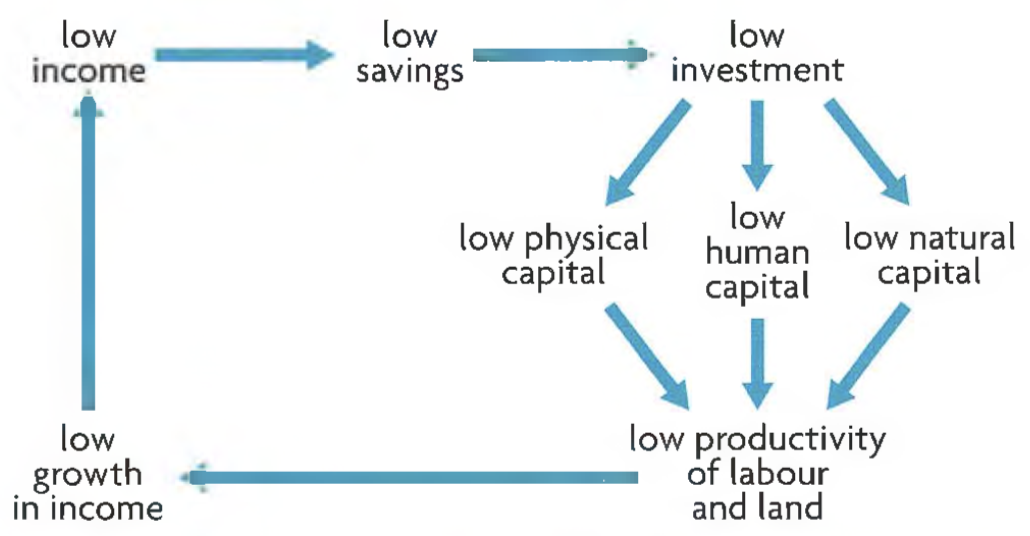
\includegraphics[width=0.5\linewidth]{Screenshot 2026-08-08 at 19.50.01.png}
\end{center}
How poverty is transmitted through generations:
\begin{itemize}
  \item People often cannot afford to send their children to school;
  \item They cannot afford the necessary medical care for themselves or for their children;
  \item Can't provide enough food
  \item They often have large families.
  \item Deplete CPR due to poverty
  \item Unable to buy modern inputs to improve productivity
  \item Can't make investments
\end{itemize}
Breaking out from the poverty cycle requires government intervention (undertake investments in human, physical, natural capital).
\subsection{Economic barriers}
The following are all barriers to economic growth:
\begin{itemize}
  \item \textbf{Economic inequality}: highly unequal income distribution is a barrier to growth --- the poor cannot invest in human/physical capital; lower-income groups spend a higher fraction of income (less saving); political control by the rich blocks redistribution. Asian Tigers (more equal distributions) grew faster than Latin American/African countries.
  \item \textbf{Limited access to infrastructure}: inadequate power, transport, telecoms, water, sanitation. Problems include:
  \begin{itemize}
    \item \textbf{Insufficient revenue}: prices charged below cost by state enterprises $\to$ insufficient funds.
    \item \textbf{Inadequate maintenance}: poor quality, unreliable services.
    \item \textbf{Limited access for the poor}: rural areas and urban slums disproportionately affected.
    \item \textbf{Misallocation of resources}: inappropriate investments (e.g.\ unused ports) while basic needs (roads, maintenance) are neglected.
    \item \textbf{Environmental neglect}: emissions, wasteful irrigation, roads/dams in ecologically vulnerable areas.
  \end{itemize}
  \item \textbf{Limited access to appropriate technology}: technologies from developed countries are often inappropriate to developing country conditions.
  \begin{itemize}
    \item \textbf{Different factor supplies}: developing countries have abundant labour but scarce capital $\to$ need labour-using technologies, not capital-intensive ones. Copying developed-country techniques (tractors, capital-intensive industry) contributed to unemployment and growth of the informal economy.
    \item \textbf{Different climate/ecological conditions}: technologies suited to temperate climates may not work in tropical/subtropical conditions (different soils, diseases, agronomic factors).
    \item \textbf{Difficulties developing appropriate technologies}: R\&D spending in developing countries is very low ($<0.5\%$ of GDP vs.\ $>2\%$ in developed countries); most innovation occurs in developed countries; intellectual property protection raises technology acquisition costs.
  \end{itemize}
  \item \textbf{Low levels of human capital} (education and health barriers):
  \begin{itemize}
    \item \textbf{Education barriers}: insufficient funding, teacher shortages, poor school facilities, gender discrimination (130M+ girls out of school), conflict (250M children in conflict zones), distance to school, hunger/malnutrition, inability to pay informal fees.
    \item \textbf{Health barriers}: insufficient health care funding (financing gap of \$370B for SDG targets), insufficient access to services (half the world lacks essential health care), private/out-of-pocket payments pushing 800M people into poverty, malnutrition, preventable diseases (malaria, HIV/AIDS, tuberculosis, diarrhoea).
  \end{itemize}
  \item \textbf{Dependence on primary sector production and exports}: many developing countries specialise in a few primary commodities (e.g.\ oil, copper, cocoa, tobacco). Risks include:
  \begin{itemize}
    \item \textbf{Price volatility of primary products}: low PED and PES $\to$ large price fluctuations $\to$ unstable export revenues, unstable incomes, uncertain investment planning.
    \item \textbf{Inability to diversify}: over-specialisation makes countries vulnerable to global recessions and falling commodity prices.
    \item \textbf{Barriers to vertical diversification} (moving into processing/manufacturing): tariff escalation by developed countries (low tariffs on raw materials, high on processed goods) discourages manufacturing.
  \end{itemize}
  \item \textbf{Limited access to international markets}:
  \begin{itemize}
    \item \textbf{Tariff barriers}: products of interest to developing countries (agriculture, textiles) face relatively high tariffs in developed countries; \textbf{tariff escalation} blocks vertical diversification.
    \item \textbf{Agricultural subsidies in developed countries}: price supports and subsidies to rich-country farmers ($\sim$\$1B/day in OECD countries) $\to$ overproduction, lower world prices, global inefficiency (US is the largest cotton exporter despite having among the highest production costs), lower export earnings and increased poverty for developing-country farmers.
    \item \textbf{Non-tariff barriers} (``new trade protection''): health/safety standards, administrative barriers, environmental standards --- sometimes used as hidden protection against developing-country exports.
  \end{itemize}
  \item \textbf{Existence of informal economy}: 61.2\% of global employment (2 billion people; 93\% in developing countries). Workers are unregistered $\to$ no labour protection, no social security, very low wages, long hours, unhealthy conditions. Government loses tax revenue. Informal employment correlates negatively with HDI and education levels; more prevalent in rural areas.
  \item \textbf{Capital flight}: financial capital leaves the country due to fears of devaluation, political instability, debt problems, or poor economic management. Effects:
  \begin{itemize}
    \item Loss of domestic investment capital.
    \item Downward pressure on the exchange rate (selling domestic currency) $\to$ forced devaluation --- often a \textbf{self-fulfilling prophecy}.
    \item Worsens foreign debt problems (increases need for external borrowing).
  \end{itemize}
  \item \textbf{Indebtedness}: many developing countries accumulated massive foreign debt (especially in the 1980s and again after 2008). Causes include:
  \begin{itemize}
    \item Global financial crisis (2008) $\to$ budget surpluses turned to deficits.
    \item Commodity price drops (2014) $\to$ lost export revenues.
    \item Low global interest rates $\to$ easier borrowing.
    \item Large infrastructure financing needs (e.g.\ Chinese loans to sub-Saharan Africa: \$125B in 2000--2017).
    \item Poor governance and exchange rate depreciation (increasing real debt value).
  \end{itemize}
  Debt servicing crowds out spending on health, education and infrastructure $\to$ deepens poverty and underdevelopment.
  \begin{itemize}
    \item \textbf{Historical background (supplementary)}: before the 1970s, developing countries borrowed only on a small scale (mainly from the World Bank, IMF and foreign governments) to supplement savings for growth and development. The debt problem began with the \textbf{1973--74 oil shock}: OPEC sharply raised oil prices, so oil-importing developing countries faced higher import bills \textit{and} lower export revenues (recessions/stagflation in developed countries reduced demand for their exports) $\to$ large current account deficits $\to$ increased foreign borrowing.
    \item Oil-exporting countries deposited their new revenues in commercial banks in developed countries; the banks then aggressively \textbf{recycled these ``petrodollars''} as loans to developing countries. Lending was often imprudent, partly because banks assumed the public sector would cover losses. Loan funds were sometimes wasted on inefficient public enterprises, low tax collection, or corruption.
    \item After the \textbf{second oil shock (1979)}, countries either borrowed more or adopted restrictive fiscal/monetary policies; by the \textbf{early 1980s}, several Latin American and sub-Saharan African countries were on the verge of bankruptcy. From \textbf{1982}, the IMF, World Bank and US government intervened to prevent defaults (see the IMF/World Bank discussion in the strategies section).
  \end{itemize}
  \item \textbf{Geography and landlocked countries}: landlocked developing countries (LLDCs) face higher transport costs, lack of direct access to seaports, dependence on transit countries, and trade barriers. 32 LLDCs globally (e.g.\ Bolivia, Chad, Mali, Nepal, Zambia). Also, overdependence on primary commodities and vulnerability to climate shocks.
  \item \textbf{Tropical climates and endemic diseases}: tropical/subtropical climates reduce soil quality, labour productivity (heat/humidity) and increase disease burden. Endemic diseases (malaria, parasitic infections, pneumonia, diarrhoea, tuberculosis, HIV/AIDS) reduce life expectancy, worker productivity, and investment in human capital. Most are preventable/curable but require resources and infrastructure that poor countries lack. Global warming is expected to worsen these effects disproportionately in poor countries.
\end{itemize}

\subsection{Political and social barriers}
\begin{itemize}
  \item \textbf{Weak institutional framework}: institutions (rules, organisations, social norms) are underdeveloped in many ELDCs. Key weaknesses include:
  \begin{itemize}
    \item \textbf{Legal framework and access to justice}: lack of effective enforcement of laws/contracts; unequal access to justice for vulnerable groups $\to$ discourages investment and economic activity.
    \item \textbf{Ineffective taxation system}: low tax revenues due to corruption in collection, bureaucratic inefficiency, tax evasion, exemptions for the wealthy/large firms, low property tax rates, and poorly designed taxes that distort resource allocation (e.g.\ favouring capital-intensive technologies, penalising medium-sized and new firms).
    \item \textbf{Banking system and access to credit}: banks prefer large, creditworthy borrowers (multinationals, manufacturing firms); poor people and SMEs lack collateral $\to$ forced into informal credit (loan sharks, pawnbrokers) at very high rates. $\sim$3 billion people lack access to basic financial services.
    \item \textbf{Property rights and land rights}: weak or non-existent property rights discourage investment. Hernando de Soto argued that land titling would unlock ``dead capital'' (using land as collateral). However, land titling often failed because:
    \begin{itemize}
      \item Western concept of private property doesn't always fit communal/traditional land systems.
      \item Titling can lead to \textbf{land grabs} --- dispossession of small farmers by large agribusinesses $\to$ undermines food security.
      \item Benefits were exaggerated; may be inappropriate for agricultural land in developing countries.
    \end{itemize}
  \end{itemize}
  \item \textbf{Lack of good governance and corruption}: corruption diverts resources away from productive uses; weakens institutions; discourages FDI; undermines tax collection; distorts public spending (favouring politically connected groups); erodes public trust. Common forms: bribery, embezzlement, nepotism, patronage, vote buying.
  \item \textbf{Unequal political power and status}: elites with economic and political power influence policies to protect their own interests $\to$ block reforms (land reform, progressive taxation, social spending) that would benefit the broader population. This creates a \textbf{vicious circle}: economic inequality $\to$ political inequality $\to$ policies favouring the rich $\to$ more economic inequality.
  \item \textbf{Gender inequality}: discrimination against women and girls in:
  \begin{itemize}
    \item \textbf{Education}: fewer years of schooling, lower literacy rates for females (especially in low-income countries); 130M+ girls out of school.
    \item \textbf{Health}: higher maternal mortality, less access to health care, nutritional disadvantages.
    \item \textbf{Economic opportunities}: lower labour force participation, lower wages, unpaid domestic/caring work, limited property/inheritance rights.
    \item \textbf{Political participation}: fewer women in parliament and decision-making roles.
  \end{itemize}
  Gender inequality is a major barrier to development $\to$ \textbf{empowerment of women} (eliminating deprivations, creating equal opportunities) produces positive externalities: better health and education for children, lower fertility rates, higher economic growth. ``Development is the best contraception'' --- as countries develop and women gain education and employment, birth rates fall.
\end{itemize}
\section{Strategies to promote EG and ED}\label{sec:strategies}
\subsection{International trade strategies}
\needbold{Import substitution (ISI)} (also known as import-substituting industrialisation) is a growth and trade strategy where a country begins to manufacture simple consumer goods (shoes, textiles, beverages, electrical appliances) for the domestic market to promote its domestic industry, using protective measures (tariffs, quotas, import licences) to keep out competing imports.
\begin{itemize}
  \item It was justified theoretically by the \textbf{infant industry argument} (protect infant domestic firms against import competition).
  \item \textbf{Typical characteristics and consequences}:
  \begin{itemize}
    \item \textbf{Heavy protection} (tariffs, quotas, import licences) $\to$ lack of competition $\to$ high costs, inefficiency, resource misallocation and high consumer prices in private and public industries.
    \item \textbf{Overvalued exchange rates} (set above the free-market level): intended to make imported capital inputs cheaper, but with two negative effects --- (i) cheap capital imports encouraged \textbf{capital-intensive, inappropriate technologies} $\to$ unemployment and growth of the urban informal economy; (ii) agricultural exports became more expensive $\to$ \textbf{worsening rural poverty}.
    \item \textbf{Extensive industrial policies and public ownership / too much govt. intervention}: subsidised credit, tax allowances, production subsidies, wage subsidies, price controls, and state ownership of fertilisers, steel, petrochemicals, cement, banking and infrastructure $\to$ serious resource misallocation and inefficiency.
    \item \textbf{Neglect of agriculture}: failed agricultural investment $\to$ increased need for food imports.
    \item \textbf{Deteriorating balance of payments}: rising capital-equipment imports, food imports, and profit repatriation by foreign MNCs.
    \item \textbf{No support for small entrepreneurs} more likely to use labour-intensive techniques $\to$ worsening unemployment, income distribution and poverty.
    \item \textbf{Negative impacts on employment and income distribution}: favor of capital-intensive production contributed to the development and growth of the informal economy, along with worsening income distribution and increasing poverty.
    \item \textbf{Limits to long run growth}: many protected firms never grew up into efficient low-cost producers; firms that should have closed down were kept alive while potentially successful ones were not created.
  \end{itemize}
  \item By the 1970s--80s, economists generally agreed ISI had not lived up to expectations, and it was largely abandoned in favour of export promotion. Today it survives only as \textbf{selective import substitution} (industrial policies for particular infant industries), not as a general growth strategy.
\end{itemize}
\needbold{Export promotion} is a growth and trade strategy where a country attempts to achieve growth by expanding exports. Like ISI, it was originally based on strong government intervention, justified by the need to develop a strong manufacturing sector oriented toward exports. In many cases the industries that became the strongest exporters were precisely those that had first received import-substituting protection.
\begin{itemize}
  \item Typical policies included:
  \begin{itemize}
    \item \textbf{Financial incentives for export industries}: targeting industries using increasingly higher skill and technology levels; investment grants, production subsidies, exemptions from tariffs on imported inputs, tax exemptions, export subsidies, and special benefits for export-oriented MNCs; incentives for private R\&D in high-technology products appropriate to local conditions.
    \item \textbf{State support}: state ownership/control of financial institutions (banking, insurance) to provide subsidised credit (lower interest rates, favourable borrowing terms); large public investments in education and skills, R\&D, and modern transport/communications infrastructure.
    \item \textbf{Regulation to maximise the benefits of FDI}: promotion of R\&D, transfer of desired technologies, training of domestic workers, use of local inputs.
    \item \textbf{Exchange-rate policies}: \textbf{undervalued currencies} that encourage exports while making imports more expensive.
  \end{itemize}
  \item \textbf{Why the Asian Tigers succeeded}: export volumes large enough to exploit \textbf{economies of scale}; \textbf{evolving specialisation} (starting with simple labour-intensive goods such as textiles, then moving to higher skill/technology levels); \textbf{macroeconomic stability}; \textbf{investment in human capital} (education, training, skills); \textbf{appropriate technologies} (labour-intensive first, then supported R\&D and technology transfer); \textbf{employment creation}; \textbf{no serious debt problems} (significant export earnings).
  \item \textbf{Problems of export promotion}: over-dependence on exports (a recession in major trading partners directly lowers AD and domestic output); pressure to keep wages low to maintain competitiveness $\to$ workers may not share the gains; persistent trade surpluses correspond to deficits in trading partners $\to$ risk of retaliatory trade protection.
\end{itemize}

\subsubsection*{Economic integration: regional vs bilateral agreements}
\begin{itemize}
  \item \textbf{Growth of trade agreements}: the number of trade agreements reported to the WTO grew from \textbf{20 in 1990} to \textbf{159 in 2007} and \textbf{270 by 2019}. Two main reasons: (i) many countries are frustrated with what they see as the \textbf{slow progress of the WTO}; (ii) developing countries see trading blocs as a way to enjoy the benefits of free trade while \textbf{bypassing rich-country trade protection}, yet still keep some of the benefits of trade protection toward non-members.
  \item \textbf{Regional FTAs} have the greatest potential to help developing countries when they involve:
  \begin{itemize}
    \item \textbf{regional agreements} among neighbouring countries;
    \item \textbf{geographical closeness};
    \item \textbf{similar levels of development and technological capabilities};
    \item \textbf{similar market sizes};
    \item a \textbf{shared commitment to co-operation}.
  \end{itemize}
  Under these conditions members can expand markets (economies of scale), diversify production and exports, attract more domestic and foreign direct investment, and face competition that is ``fair'' --- no firm enjoys an unfair advantage from much more advanced technology, managerial know-how or a larger home market. With shared commitment to co-operation, members can jointly invest in transport infrastructure, energy and water supplies, collaborate on R\&D and new technology development, and work together on environmental issues of common interest. These factors greatly increase the likelihood that integration leads to growth and development. 
  \item \textbf{Bilateral FTAs} (mostly between a developing country and a developed country --- the US, the EU acting as a unit, or Japan --- usually not in the same geographical region) offer the \textbf{prospect of access to the developed country's market}, which is why developing countries enter them. But they carry serious risks:
  \begin{itemize}
    \item the developing country must make \textbf{equal and matching tariff cuts}, often far greater than WTO agreements require $\to$ even efficient local firms are put at a competitive disadvantage against lower-cost developed-country firms, and may be destroyed;
    \item when \textbf{many developing countries sign FTAs with the same developed country}, each loses its hoped-for individual advantage because they must now compete with each other for the same market $\to$ limited export gains;
    \item increased imports with only slightly increased exports $\to$ \textbf{trade deficits, balance of payments problems and increasing foreign debt}, plus greater unemployment, worsening income distribution and increased poverty;
    \item \textbf{weaker bargaining power} than in the WTO, where developing countries can present their interests together;
    \item additional requirements that may not be in the country's best interests (e.g.\ freer rules on foreign direct investment, stricter copyright and patent laws);
    \item bilateral agreements \textbf{divide developing countries} and weaken regional trade agreements when a member country signs a bilateral deal with a third country.
  \end{itemize}
  Developing countries are generally \textbf{better off pursuing regional trade agreements}. 
\end{itemize}

\subsection{Diversification and social enterprise}
\needbold{Diversification} involves a reallocation of resources into new activities that broaden the range of goods or services produced. As a country grows, the relative share of the primary sector in GDP shrinks and is progressively replaced by manufacturing and later services; exports become more varied accordingly.
\begin{itemize}
  \item \textbf{Value added and higher value-added production}: value added is the value added at each step of a production process (e.g.\ cocoa beans $\to$ cleaned/roasted/shelled $\to$ cocoa liquor $\to$ cocoa butter and cocoa powder $\to$ chocolate). A country that processes its raw materials rather than exporting them in raw form:
  \begin{itemize}
    \item engages in more varied production activities;
    \item creates employment opportunities;
    \item establishes new manufacturing firms;
    \item expands into activities requiring higher skill and technology levels.
  \end{itemize}
  Exporting primary commodities in raw form traps the country in stagnant production methods with limited prospects for change.
  \item \textbf{The natural resource curse}: since the 1960s, resource-\textit{poor} developing countries have grown faster than resource-rich ones. Countries such as Russia, Nigeria, Mexico, Venezuela, Congo, Sierra Leone and South Africa experienced low or negative growth despite abundant resources. Explanation: resource-poor countries had to diversify early into labour-intensive manufacturing, human capital and appropriate technologies, while resource-rich countries became dependent on primary commodities $\to$ volatile export revenues, external borrowing, large debts and BoP difficulties.
  \item \textbf{Benefits of diversification}:
  \begin{itemize}
    \item \textbf{Sustained export growth}: commodity exports cannot satisfy the need for markets with sustained global demand growth.
    \item \textbf{Incentives for technology, training, education and skills} (a factor behind the Asian Tigers' success).
    \item \textbf{Reduced vulnerability} to fluctuating export prices.
    \item \textbf{Use of domestic raw materials} as the base for manufacturing (successful examples: Malaysia, Thailand, Indonesia, China, Chile, Mauritius).
  \end{itemize}
  \item \needbold{Social enterprise}: a type of commercial organisation that aims to achieve social goals to improve people's well-being and promote social change. It may be for-profit or not-for-profit; if for-profit, its primary objective is its social goals, not profit maximisation. It tries to be \textbf{commercially viable} (covering all costs through sales) rather than rely on grants, and any profits are reinvested rather than distributed to owners. Social enterprises operate in education, health, social care, agriculture, fisheries, forestry, energy, clean technology and transport; most workers are relatively young with high female participation. \textbf{Microfinance} is considered a type of social enterprise (Muhammad Yunus used the term for his work with the Grameen Bank).
\end{itemize}

\subsection{Market-based policies}
\textbf{Background}: the spectacular success of the Asian Tigers contrasted sharply with the poor export/growth performance and heavy indebtedness of many other developing countries in the early 1980s. At that time monetarist/new classical ideas emphasising limited government intervention and competitive free markets became influential, producing the \needbold{Washington Consensus} (so called because it was shared by the World Bank, the IMF, the US Congress and US agencies, all based in Washington, DC).
\begin{itemize}
  \item \textbf{Main policies recommended}:
  \begin{itemize}
    \item \textbf{Trade liberalisation}: move to free trade by lowering and eliminating tariffs and other trade barriers.
    \item \textbf{Privatisation} of state-owned enterprises (transport, oil, gas, utilities).
    \item \textbf{Deregulation of labour and product markets}: market-based supply-side policies for labour (reducing union power and unemployment benefits, reducing or eliminating minimum wages) and removal of barriers to entry in product markets.
    \item Additional measures: encourage \textbf{floating exchange rates}; reduce restrictions on FDI by MNCs; limit government borrowing and keep budget deficits under control; restrict the use of industrial policies.
  \end{itemize}
  \item Countries that increasingly adopted liberalising policies from the 1980s include Argentina, Brazil, China, Chile, India, Kenya, Sri Lanka, Tanzania, Turkey and many East Asian countries --- usually as a gradual reduction of intervention, not a complete abandonment.
\end{itemize}
\textbf{Results by the 1990s} --- the expected benefits did not materialise:
\begin{itemize}
  \item \textbf{Lost export share}: many countries (losses greatest in Africa) saw their share of world exports fall. The UNDP estimated that if Africa had kept its 1980 share of world exports into the early 2000s, its exports would have been US\$119 billion greater --- about five times the aid provided by donors in 2002.
  \item \textbf{Failure to diversify into manufacturing}: in 2000, just five developing countries accounted for two-thirds of developing-country low-technology manufactured exports, and six for over four-fifths of medium- and high-technology manufactured exports; manufacturing export growth was low or moderate in most Latin American and African countries, and its relative share even fell in some.
  \item \textbf{The countries that fared best were those that already had significant export sectors} (the East Asian countries) --- whose earlier success was itself built on strong government intervention and industrial policies.
  \item \textbf{No clear link between liberalisation and growth}: well-known development economists concluded there is little evidence that open trade policies are significantly associated with faster growth, and the most comprehensive assessment found no clear link.
  \item \textbf{Increased inequality and poverty}: a World Bank study found trade liberalisation led to lower income growth for the poorest 40\% of the population and higher income growth for higher-income groups --- ``it helps the rich get richer and the poor get poorer.''
\end{itemize}
\textbf{Winners and losers from liberalisation}:
\begin{itemize}
  \item \textbf{Winners}: workers in new export industries; those finding jobs in a growing formal sector; educated and skilled workers able to exploit new opportunities.
  \item \textbf{Losers}: less educated/illiterate people unable to compete; poor people without collateral and access to credit; people in remote areas without transport links; people with nothing to export; farmers switched to commodity production for export (more vulnerable to price volatility); public-sector employees laid off as government shrinks; private-sector workers whose firms close against imports; workers fired in privatised enterprises; people hurt by cuts in merit-good spending and lower social protection; people forced into the informal economy (e.g.\ formal employment in Zambia fell by 15\% in the 1990s).
  \item Trade theory argues that since overall gains exceed overall losses, gainers could compensate losers so no one is worse off --- but in the real world such compensation rarely (if ever) takes place. Joseph Stiglitz (former World Bank Chief Economist) criticised the ``neoliberal'' model for focusing excessively on market liberalisation while ignoring its distributional and human costs.
\end{itemize}
\textbf{The new (post-Washington) consensus} (since the late 1990s) holds that developing countries need a \textbf{mix of markets and government intervention}:
\begin{itemize}
  \item governments should support \textbf{education, health services, infrastructure development, R\&D and technology transfer} (for both industry and agriculture);
  \item large budget deficits should be avoided, but contractionary fiscal policy should \textbf{not cut education, health and infrastructure spending};
  \item policy should pay attention to \textbf{income distribution} and promote equity and poverty alleviation;
  \item governments must provide a proper \textbf{regulatory framework} (e.g.\ effective competition regulation so privatisation does not create private monopolies);
  \item efforts are needed to build \textbf{institutions}: property and land rights, an effective tax system, and an effective banking/credit system;
  \item developed countries must support development by \textbf{increasing foreign aid} and \textbf{opening their markets} to developing-country exports, including special treatment under WTO rules (e.g.\ removing rich-country agricultural protection);
  \item in short: \textbf{government intervention is important to create the conditions for markets and trade to work in favour of developing countries}.
\end{itemize}

\subsection{Interventionist policies: redistribution and provision of merit goods}
\textbf{Taxation policies} (SDG 17.1: strengthen domestic resource mobilisation and tax collection). The IMF recommends developing countries:
\begin{itemize}
  \item increase the \textbf{progressivity} of the tax system (usually lower than in developed countries);
  \item gradually \textbf{expand the coverage of personal income taxes};
  \item expand \textbf{indirect taxes on luxury goods and goods creating negative externalities} (cigarettes, alcohol, fossil-fuel energy);
  \item increase taxation of \textbf{capital income (profits)} --- essential for progressivity;
  \item impose or increase taxes on \textbf{real estate and land};
  \item take measures to \textbf{reduce tax evasion}.
\end{itemize}
\textbf{Transfer payments} (SDG 1.3: nationally appropriate social protection systems with floors, covering the poor and vulnerable by 2030). The World Bank and ILO call for \textbf{universal social protection} (child benefits, old-age pensions, maternity, disability, work-injury and unemployment benefits) by 2030.
\begin{itemize}
  \item In 2019, \textbf{more than half the world's population (4 billion people) had no access to even one social protection benefit}; 45\% had access to one benefit, one-third of children had a family/child benefit, only 28\% of people with disabilities had a benefit, and old-age pensions were the most prevalent (68\% of older persons).
  \item Benefits (mostly cash transfers or benefits in kind): reduce poverty and encourage social inclusion; empower individuals to make decisions reflecting their own preferences; raise demand for locally produced goods; promote growth via higher incomes/consumption/investment (AD); provide safety against emergencies; improve access to health care and education; encourage women's empowerment and delayed marriage; reduce malnutrition and child mortality; bring the poor into the formal economy; reduce child labour; build political stability; and --- according to numerous studies --- do \textbf{not} reduce adults' incentive to work.
  \item \textbf{Conditional cash transfers (CCTs)} pay money on condition that households undertake education/health-care activities (often for children); non-conditional transfers give households flexibility. There is no consensus yet on which type is more successful.
  \item Implementation difficulties: universal systems are costly, may exceed developing-country budgets in the short term; effectiveness depends on complementary government provision of schools, hospitals, roads, clean water, sanitation and trained health workers; design problems can prevent money reaching those most in need.
\end{itemize}
\textbf{Minimum wages}: standard theory predicts unemployment, but a growing number of studies show such job losses \textbf{do not occur unless minimum wages are set at very high levels}; since the late 1990s many countries have introduced or raised minimum wages as an anti-inequality policy. Policy-design guidance (IPC-IG): set minimum wages after consulting workers and employers; consider workers' and families' needs; monitor and evaluate effects; build in regular review (every year or two); establish compliance and enforcement measures to avoid work below the legal minimum.
\\
\textbf{Provision of merit goods: education} (SDG 3, SDG 4, SDG 1.A.2). Education has large positive externalities:
\begin{itemize}
  \item contributes to \textbf{economic growth} via higher labour productivity and output;
  \item improves the quality of physical capital (knowledge applied to R\&D, especially \textbf{appropriate technology} for local economic, ecological and climate conditions);
  \item lowers unemployment and absenteeism, increases international competitiveness and attracts FDI;
  \item increases political stability;
  \item lowers crime rates and improves quality of life;
  \item education of women raises labour-force participation and lowers birth rates/population growth;
  \item spillovers into health: education of women improves maternal health and lowers maternal and child mortality; schools teach hygiene and sanitation.
\end{itemize}
The successful East Asian countries invested more heavily in education than comparable countries, beginning with \textbf{universal literacy} and only later expanding secondary and tertiary education in line with technological capability. A common misallocation in developing countries is investing too heavily in higher education while ignoring primary education:
\begin{itemize}
  \item \textbf{International brain drain}: university graduates migrate to developed countries $\to$ poor-country resources build human capital in rich countries;
  \item \textbf{Internal brain drain}: highly educated people work in unrelated lower-skill jobs (a doctor driving a taxi); doctors trained in public institutions work in the private sector instead of serving low-income groups; researchers focus on developed-country problems rather than local technological needs.
\end{itemize}
\textbf{Provision of merit goods: health care}. Health also has external benefits: greater worker productivity and output; less disease transmission; immunisation protects the community; healthier people participate more actively; better health improves school attendance/performance, makes better use of knowledge and skills, and lengthens the productive lifespan.
\begin{itemize}
  \item Appropriate intervention is mainly \textbf{direct government provision free of charge}: an estimated \textbf{100 million people are pushed into extreme poverty} by having to pay for health care, and many die unnecessarily because they cannot afford it.
  \item Complementary investments: sanitation, clean water and sewerage; legislation making education compulsory; advertising/persuasion/nudges for immunisation and preventive care (useless if no schools or clinics exist).
  \item Oxfam's principles for public services: \textbf{universal}; \textbf{free at the point of use}; \textbf{public} (government-provided); able to \textbf{prioritise services important to women} and promote women as workers; and \textbf{accountable} to those they serve.
\end{itemize}
\textbf{Provision of infrastructure} (SDG 6: water and sanitation; SDG 9: resilient infrastructure, inclusive industrialisation and innovation):
\begin{itemize}
  \item Infrastructure raises \textbf{productivity} and lowers production costs: roads/rail save transport time; telecommunications speed communication; irrigation raises yields and expands agricultural output; electricity allows simple powered machinery; safe water, sanitation and sewerage support health and enable diversification into processed foods.
  \item Infrastructure determines a country's \textbf{international competitiveness} (shipping costs) and \textbf{attracts FDI}.
  \item Transport brings remote rural people closer to education/health facilities, creates employment (especially when built with labour-intensive methods), and integrates isolated areas into the market economy.
  \item Water and energy infrastructure have major effects on \textbf{gender equity}: without piped water, electricity or gas, women and girls spend a large share of time (up to two-thirds of household time in some African countries) carrying water and fuel; providing these services frees time $\to$ higher girls' school enrolment, women's outside employment, and lower fertility.
  \item Safe energy sources reduce \textbf{indoor air pollution} (from burning polluting fuels), with strong health benefits for women and children.
\end{itemize}

\subsection{Foreign direct investment and multinational corporations (MNCs)}
\needbold{Foreign direct investment (FDI)} is investment by firms based in one country (the \textbf{home} country) in productive activities in another country (the \textbf{host} country), with control of at least \textbf{10 per cent} of the firm in the host country. A firm that undertakes FDI is a \needbold{multinational corporation (MNC)} --- it operates in more than one country; a corporation is a legal entity separate from the individuals who own it.
\begin{itemize}
  \item \textbf{Scale and history}: MNCs have operated since about the mid-19th century; their importance grew in the 1950s (US multinationals investing in European post-war reconstruction) and exploded in recent decades: from an estimated 37\,000 MNCs in the early 1990s to 82\,000 by 2009, employing 80 million people in foreign affiliates. The top ten non-financial MNCs had revenues above US\$2.7 trillion in 2017. MNCs produce an estimated \textbf{33\% of global output} (about two-thirds at home, one-third in foreign affiliates) and account for more than half of world exports and nearly half of imports. FDI remains a small share of total private investment in developing countries (local firms invest far more), but it is \textbf{qualitatively different} because of MNCs' huge size, economic/political power and superior technology/management. FDI is the most important source of foreign finance flows to developing countries as a whole --- though many low-income countries are almost completely bypassed, so \textbf{foreign aid} is their main source of foreign finance.
  \item \textbf{Why MNCs expand into developing countries}:
  \begin{itemize}
    \item \textbf{Investment opportunities}: large or rapidly growing markets (China, India, Latin America) offer potential for big sales increases.
    \item \textbf{Bypassing trade barriers}: producing inside a country with trade barriers secures access to its market.
    \item \textbf{Lower labour costs} (labour is a large share of production costs).
    \item \textbf{Use of local raw materials} (cheaper than importing them).
    \item \textbf{Natural resource extraction} (oil, aluminium, bauxite) in resource-rich developing countries.
  \end{itemize}
  \item \textbf{What MNCs seek in a host country}: political stability; a stable macroeconomic environment (low inflation, stable currency, acceptable foreign debt, no major BoP problems); favourable tax rules; weak labour protection laws; a liberalised economy and trade policy with an export emphasis; large markets; rapid growth; well-functioning infrastructure (transport, communications); and a well-educated labour force.
  \item \textbf{Advantages for host countries}:
  \begin{itemize}
    \item \textbf{Capital inflow}: FDI credits in the financial account can offset a current account deficit; export-oriented MNCs raise export earnings.
    \item \textbf{Technology and managerial transfer}: local workers and businesses can learn and adopt new production technologies and management practices.
    \item \textbf{Supplementing domestic savings} for investment.
    \item \textbf{Tax revenues} (if MNCs are taxed).
    \item \textbf{Linkages with local industry}: buying local inputs promotes the growth of existing firms and the creation of new ones.
    \item \textbf{Employment} from hiring local workers.
    \item \textbf{Growth and development} via investment, technology, human capital and tax revenues.
  \end{itemize}
  \item \textbf{Disadvantages}:
  \begin{itemize}
    \item \textbf{Small net foreign-exchange inflows}: profit repatriation, imports of raw materials/inputs, and repayment of loans from the parent corporation offset the initial capital inflow.
    \item \textbf{Limited technology/skill transfer}: links with the local economy are often limited, and MNCs often hire personnel from the home country.
    \item \textbf{Transfer pricing}: MNCs buy inputs from their own affiliates and overstate the prices paid, understating profits and taxes; lost tax revenues are estimated in the billions of dollars annually.
    \item \textbf{Crowding out}: MNC operations may force local competing firms out of business or prevent new local firms from entering.
    \item \textbf{Limited job creation}: prevention of local industry development, plus capital-intensive (inappropriate) technologies, can contribute to unemployment and growth of the informal economy (though some MNCs use labour-intensive methods).
    \item \textbf{Environmental damage}: MNCs prefer countries with few environmental restrictions; a Union Carbide plant explosion in India (1984) killed over 20\,000 and left 100\,000+ with permanent health problems; since 1988, 100 MNCs are estimated responsible for over 71\% of greenhouse gas emissions.
    \item \textbf{Inappropriate consumption patterns}: advertising creates new consumption needs (soft drinks, sweets, fast food, brand-name goods) that poor populations can ill afford.
    \item \textbf{Infrastructure demands}: host countries may shift scarce resources away from merit goods (clean water, sanitation, schools, health care) toward infrastructure needed to attract MNCs.
    \item \textbf{Political power and weak bargaining position}: MNCs can pressure host governments for policies in their own interest (e.g.\ Peru: a mining company pressed the government not to conduct children's health tests near its operations); governments fear losing the investment to other countries.
    \item \textbf{Race to the bottom}: developing countries compete to offer ever-better conditions to attract MNCs, sacrificing policies needed for growth and development.
  \end{itemize}
\end{itemize}

\subsection{Foreign aid}
\needbold{Foreign aid} is the transfer of funds or goods and services to developing countries with the main objective of bringing about improvements in their economic, social or political conditions. To count as aid, transfers must be:
\begin{itemize}
  \item \textbf{concessional} --- on more favourable conditions than the market (loans have lower interest rates and longer repayment periods than commercial borrowing; aid may also involve \textbf{grants}, gifts of money or goods/services that do not need repayment);
  \item \textbf{non-commercial} --- not involving buying, selling or profit-making activities.
\end{itemize}
Military aid, peacekeeping and refugee assistance are \textbf{not} counted as foreign aid (they are not directly concerned with improving developing countries' economic, social or political conditions).
\begin{itemize}
  \item \textbf{Types of aid}:
  \begin{itemize}
    \item \textbf{Humanitarian aid}: for emergencies caused by violent conflicts or natural disasters (floods, earthquakes, tsunamis); saves lives, ensures access to food, water, shelter and health care, and assists reconstruction; delivered through grants or goods-in-kind (food, medical supplies, blankets).
    \item \textbf{Development aid}: intended to help countries achieve growth and development objectives; may involve financial support for specific projects (schools, clinics, hospitals, irrigation), sectoral support (education, health, agriculture, energy, environment), \textbf{technical assistance} (specialists such as doctors, teachers, agronomists), and \textbf{debt relief}; delivered through grants, concessional long-term loans and debt forgiveness.
  \end{itemize}
  \item \textbf{Sources of aid}:
  \begin{itemize}
    \item \textbf{Official Development Assistance (ODA)}: public funds from donor governments; the largest part of foreign aid, with nearly three-quarters taking the form of grants. ODA reaches recipients (i) \textbf{bilaterally} (directly, e.g.\ USAID in the US, DFID in the UK --- the most important channel), (ii) \textbf{multilaterally} (through international organisations: UN agencies, the Global Fund to Fight AIDS, Tuberculosis and Malaria, the IDA, regional development banks, IMF debt-relief assistance), or (iii) \textbf{through NGOs}. Donors include most OECD members, some OPEC members and some Eastern European countries.
    \item \textbf{Non-governmental organisations (NGOs)}: private organisations pursuing activities to relieve suffering, promote the interests of the poor, protect the environment, provide basic social services, or undertake community development (World Bank definition). They are part of civil society --- the ``third sector'' alongside government and markets. Examples: Amnesty International, Greenpeace, Oxfam, Save the Children, WWF. NGOs obtain funds from private voluntary contributions and increasingly from bilateral/multilateral ODA (especially for humanitarian assistance). Their activities include humanitarian aid, sustainable development, community development, service delivery, poverty alleviation, child health, women's rights, small-scale entrepreneurship, informal-sector support, technical assistance to small farmers, \textbf{microfinance}, research, political advocacy and support for people's movements.
  \end{itemize}
  \item \textbf{Donor motives}: political/strategic (during the Cold War the US aided countries to restrict the spread of communism, the USSR aided communist states; European powers aided former colonies; aid has supported friendly regimes); economic (supporting countries with strong trade/investment links, e.g.\ much of Japan's aid goes to neighbouring countries; \textbf{tied aid} is an economic motive); and humanitarian (emergency relief and long-term poverty-reduction concern). As a result, aid does \textbf{not} go to the countries that need it most --- developing countries with poor governance and little strategic/economic importance receive disproportionately less aid.
  \item \textbf{Why aid matters (arguments in favour)}:
  \begin{itemize}
    \item allows poor countries to \textbf{escape the poverty cycle} by funding investments in physical, human and natural capital that tax revenues cannot finance;
    \item funds health, education and infrastructure even when a country is not in a poverty cycle, improving employment opportunities and incomes;
    \item can improve \textbf{income distribution} by focusing on the most disadvantaged groups;
    \item there is strong evidence that aid \textbf{contributes to growth} (by raising investment and consumption);
    \item aid is crucial for achieving the \textbf{SDGs} --- the UNDP states developing countries cannot achieve them without sufficient aid;
    \item \textbf{debt relief} reduces debt burdens and frees resources for poverty reduction and development.
  \end{itemize}
  \item \textbf{Factors limiting aid effectiveness}:
  \begin{itemize}
    \item \textbf{Tied aid}: donors require recipients to spend all or part of the funds buying goods/services from the donor country (only possible with bilateral aid). Disadvantages: recipients cannot shop for lower-price alternatives and therefore face higher-than-necessary import costs; forced purchases often involve inappropriate, capital-intensive technologies; the main beneficiaries are large firms in donor countries.
    \item \textbf{Conditionality}: donors impose conditions (greater market orientation --- privatisation, elimination of trade barriers --- or particular projects). Disadvantages: donor preferences override recipient/population preferences; policy prescriptions may be wrong or incompatible with the government's development strategy; conditions weaken recipient government authority and accountability to citizens.
    \item \textbf{Volatility and unpredictability}: aid flows (especially bilateral) change with donor budgets and priorities $\to$ recipients cannot plan investments; aid cuts can devastate basic services in highly aid-dependent countries.
    \item \textbf{Lack of co-ordination}: many uncoordinated donors finance hundreds of overlapping or inconsistent projects, producing inefficiency and incoherence.
    \item \textbf{Substitution for domestic resources}: recipients may use aid to substitute for tax effort instead of supplementing domestic resources (evidence is mixed).
    \item \textbf{Allocation not based on need}: donors allocate by their own interests (aid as ``carrot and stick''), recipients may lack commitment or expertise for poverty alleviation, and tied aid favours inappropriate projects.
    \item \textbf{Corruption}: misuse of aid funds by recipient governments.
    \item \textbf{Insufficient quantity}: donors have repeatedly promised 0.7\% of GNI as ODA, but only a few meet the target --- and those that fail include the largest/richest donors.
  \end{itemize}
  \item \textbf{NGO strengths}: reach the very poor more effectively than governments; work closely with beneficiaries and involve local people in project design/implementation (ownership and commitment); contribute to \textbf{democratisation} by giving poor people political voice; accumulate cross-country experience; can be more creative, innovative and independent (not subject to conditionality or tied aid); and often enjoy greater trust than governments.
  \item \textbf{NGO weaknesses}: may be too small/weak with limited resources and difficulty attracting skilled personnel; may lose independence as they become dependent on funders; may poach scarce highly qualified personnel from governments; and their advocacy role can conflict with governments. The consensus view is favourable, but NGOs must act \textbf{in partnership with governments}, not replace them --- governments alone can provide the overall policy framework, legal/institutional/regulatory framework, economic stability and market-failure correction.
  \item \textbf{Debt relief}: following the 1982 debt crisis, the international community responded with \textbf{debt restructuring} (new commercial-bank loans stretched over longer periods at lower interest rates), plus \textbf{conditional loans} from the IMF (tight fiscal/monetary policies, liberalisation, market-based supply-side policies) and World Bank (economic/trade liberalisation). In 1996 the World Bank and IMF launched the \textbf{Heavily Indebted Poor Countries (HIPC) Initiative} to cancel part of the external debts of the poorest highly indebted countries; in 2005 the \textbf{Multilateral Debt Relief Initiative (MDRI)} provided 100\% debt relief on debts owed to the World Bank, IMF and other multilateral institutions. Eligibility requires: income per capita below a threshold; an unsustainable debt level (debt trap); evidence of following certain IMF/World Bank policies (spending cuts, market liberalisation); and commitment to a poverty-reduction strategy. By 2019, 39 countries were eligible and 36 had received full debt relief.
  \begin{itemize}
    \item \textbf{Benefits of HIPC relief}: savings from cancelled debt must be spent on attacking poverty (rural infrastructure, health services, education, new jobs, family planning); debt reduction is embedded in a broader development effort, so social spending averages about \textbf{five times} the debt-service payments saved.
    \item \textbf{Criticisms}: some bilateral creditors have not provided relief and participation is voluntary; the programme acts too slowly; qualifying conditions can be severe (school/hospital fees, privatisation of key public enterprises, cuts in social services and infrastructure); and many highly indebted countries that are ``not poor or indebted enough'' to qualify still suffer the consequences of high debt without relief.
  \end{itemize}
\end{itemize}

\subsection{Multilateral development assistance}
Multilateral development assistance involves lending to developing countries on \textbf{non-concessional} terms (interest rates and repayment periods determined in the market). The major multilateral lenders are the \textbf{multilateral development banks} (World Bank, African Development Bank, Asian Development Bank, Inter-American Development Bank, European Bank for Reconstruction and Development) and the \textbf{IMF}. Unlike commercial banks, they lend for economic development or international financial stability rather than for profit.
\begin{itemize}
  \item \textbf{The World Bank} (established 1944 to help reconstruct Europe; activities extended to developing countries from the late 1950s; 189 member states as joint owners):
  \begin{itemize}
    \item \textbf{Structure}: the \textbf{IBRD} lends on non-concessional (commercial) terms to middle-income developing countries --- about 75\% of Bank lending, so most of the World Bank is \textbf{not} an aid agency; the \textbf{IDA} (established 1960) lends to low-income countries on highly concessional terms. Three additional organisations (IFC, ICSID, MIGA) focus mainly on private investment in developing countries.
    \item \textbf{History}: initially lent for \textbf{infrastructure} (energy, transport, telecommunications, irrigation); by the early 1970s it turned to \textbf{poverty alleviation} (helping the poorest 40\% of populations via water, sanitation, education, health, employment projects); in the late 1970s--80s it shifted to \textbf{structural adjustment loans (SALs)} --- loans conditioned on removing price controls, liberalising interest rates and trade, removing FDI restrictions, privatisation, deregulation and cutting government spending --- which came under strong criticism by the 1990s; since the mid-1990s it has returned to a \textbf{poverty orientation} (MDGs, now SDGs; environmentally sustainable projects; a new view that governments must intervene in education, health, infrastructure, credit access, land reform, environmental degradation, poverty cycles and gender equity) and stresses \textbf{institutional development} (education/health services, infrastructure, effective taxation, credit access, property/land rights, corruption control, women's empowerment, appropriate technology, political voice for the economically weak, competition).
    \item \textbf{Criticisms}: early socially unsound projects (hydroelectric dams displacing indigenous people) and environmentally unsustainable projects; governance is weighted by financial contributions, giving rich countries far greater power; excessive interference in domestic policy; conditionality deprives countries of control over domestic economic activities; insufficient funds for poverty-oriented lending and for HIPC debt relief; the 2019 \textit{World Development Report} was criticised by the ILO for excessive focus on labour-market flexibility and for ignoring negative effects on workers; and it has been criticised for encouraging land grabs through privatisation and land takeovers that displace poor farmers.
  \end{itemize}
  \item \textbf{The International Monetary Fund (IMF)} (established jointly with the World Bank in 1944; 189 members):
  \begin{itemize}
    \item \textbf{Purpose}: oversee the global financial system; follow member countries' macroeconomic policies; stabilise exchange rates; and help countries with international payments difficulties by extending \textbf{short-term loans on commercial (non-concessional) terms}. Its original purpose was lending to countries with BoP deficits under the fixed-exchange-rate system.
    \item \textbf{History}: in its first two decades over half its lending went to developed countries; its role in developing countries grew with the 1970s--80s debt crisis (oil-importing poor countries with serious BoP difficulties); in the 1990s it lent to transition economies (central/eastern Europe, former Soviet Union); since 2008 lending has increased sharply due to the global financial crisis, including to developed countries (Greece, Iceland, Ireland, Portugal).
    \item \textbf{Stabilisation policies} (typical conditions): \textbf{contractionary monetary policy} (higher interest rates to lower AD, reduce imports and attract capital inflows); \textbf{contractionary fiscal policy} (cuts in government spending --- including merit goods, food subsidies --- tax increases, and fees for schooling/health care); \textbf{currency devaluation/depreciation}; \textbf{real wage cuts} (market-based supply-side policy); and \textbf{liberalisation policies} (removing price, interest-rate, import and foreign-exchange controls).
    \item \textbf{Criticisms}: governance weighted toward rich countries; excessive interference in domestic economies; harsh conditions running counter to growth/development objectives; stabilisation policies lower growth and create recession, unemployment and poverty (cuts in real wages, merit goods and food subsidies, and school/health fees impose huge human costs); and the approach may be fundamentally wrong --- many countries following IMF programmes suffer low or negative growth and cannot grow out of BoP/debt problems.
    \item \textbf{Recent moderation}: an IMF article (\textit{Neoliberalism: Oversold?}) acknowledged that some neoliberal policies increased inequality rather than delivering growth; that benefits for growth are difficult to establish; that the costs in inequality are prominent; and that inequality hurts the level and sustainability of growth.
  \end{itemize}
\end{itemize}

\subsection{Institutional change}
\begin{itemize}
  \item \needbold{Microfinance / microcredit} (SDG 1.4): credit in small amounts to people who do not ordinarily have access to credit --- ``micro'' refers to the small loans, the very small businesses financed (\textbf{micro-enterprises}), and the short repayment periods.
  \begin{itemize}
    \item Delivered by \textbf{microfinance institutions (MFIs)}: credit unions, financial NGOs, informal savings and loan groups, and some commercial banks with special programmes for the poor.
    \item History: first appeared in the 1970s as experimental programmes lending tiny amounts to groups of poor women lacking collateral; repayment was enforced by a \textbf{group guarantee} (each member guarantees every other member). Programmes expanded in the 1980s--90s and revealed that the poor (especially women) have excellent repayment rates and can pay interest high enough for MFIs to cover costs.
    \item Borrowers: micro-entrepreneurs (street vendors, carpenters, seamstresses --- mostly in the informal economy), landless rural workers, small farmers, female heads of households, pensioners and displaced persons. MFIs tend to target women because women are more likely to repay and more likely to use earnings to improve family well-being.
    \item Criticisms/dangers: microcredit must not substitute for complementary government policies (provision of merit goods, infrastructure, and protection for disabled/ill/displaced people --- poor people should not have to borrow for health care and education); it encourages growth of the unregulated informal economy; the poorest of the poor often lack even basic literacy/numeracy skills, so loans can become a burden (some schemes integrate credit with education); and interest rates are high relative to market rates because very many very small loans are costly to provide --- some argue subsidies are needed for the poorest borrowers, but donor funds are insufficient and unreliable.
    \item A well-known example is the \textbf{Grameen Bank} in Bangladesh, which provides credit to poor people without collateral.
  \end{itemize}
  \item \textbf{Mobile banking}: using mobile phones to send/receive money and pay bills. \textbf{53\% of adults globally lack access to formal financial services} (80\% in sub-Saharan Africa, 65\% in Latin America, 68\% in the Middle East, 59\% in East/Southeast Asia, 58\% in South Asia, vs 8\% in high-income OECD countries); in most developing countries more people have phones than bank accounts. Advantages: instant payments with no delays; no need to travel long distances holding cash (theft risk); lower transfer costs; stronger rural--urban links; easier to pay workers delivering aid to remote areas; easier access to loans, insurance and business services; easier instalment payments for equipment; helps women expand beyond subsistence farming into small businesses; easier purchase of inputs; and overall a major contribution to poverty reduction. Challenges: network problems; cost relative to very low incomes; and inability of some older illiterate people to use services (fraud risk).
  \item \textbf{Women's empowerment} (SDG 5): women account for half the world's population but 70\% of the world's poor and earn about 10\% of world income. External benefits of women's education/income:
  \begin{itemize}
    \item \textbf{children's health}: more educated women and higher women's incomes improve children's health, nutrition and survival much more than equivalent improvements in men's same aspects;
    \item \textbf{children's education}: more educated mothers raise more educated children;
    \item \textbf{quality of human resources}: these effects accumulate over years, profoundly affecting growth, development and human development, and help families break the poverty cycle;
    \item \textbf{lower population growth}: more education, work outside the home and higher incomes lead to later marriage and greater reproductive choice $\to$ fewer children.
  \end{itemize}
  Amartya Sen views women as ``active agents of change''; the UNDP measures gender gaps with the \textbf{Gender Inequality Index (GII)}. Policies (UNFPA): equal political participation/representation; education, skill development and employment with priority to eliminating poverty, illiteracy and poor health; income-earning beyond traditional occupations with equal labour-market rights; eliminating violence and all discrimination against women; and enabling women to combine childbearing/child-rearing with labour-force participation.
  \item \textbf{Reducing corruption} (SDG 16.5): requires political will to create strong fiscal institutions promoting integrity and accountability throughout the public sector. Recommended policies: high \textbf{transparency} and independent external scrutiny (e.g.\ online platforms in Colombia, Costa Rica and Paraguay let citizens monitor public investment projects); \textbf{reform of tax administration}; a \textbf{professional civil service} based on transparent, merit-based hiring and pay; focus on \textbf{high-risk areas} (procurement, revenue administration, natural-resource management); and \textbf{cross-border cooperation} (40+ countries have made it a crime for companies to bribe foreign officials). The World Bank supports anti-corruption by establishing institutions/incentives to prevent corruption, creating penalties and sanctions, and influencing governance perceptions.
  \item \textbf{Property rights and land rights} (SDG 1.4.2): titling encourages investment and facilitates credit, and can be successful in urban areas, but Western-style private titling may not fit land based on custom or communal use. Secure land rights:
  \begin{itemize}
    \item contribute to \textbf{food security} (improved sustainable land use, credit access, productivity of small farmers);
    \item lead to \textbf{lower rates of deforestation};
    \item preserve \textbf{diverse food cultures and biodiversity};
    \item support \textbf{indigenous peoples} and improve their economic/social status;
    \item contribute to \textbf{gender equality} when granted to women;
    \item contribute to \textbf{poverty reduction}.
  \end{itemize}
  In 2012 the FAO (with civil society, the private sector and research institutions) established the \textbf{Voluntary Guidelines on the Responsible Governance of Tenure of Land, Fisheries and Forests} --- first-ever global guidelines on land tenure, including recording individual and collective tenure rights, systems for maintaining/publicising rights, dispute-resolution mechanisms, anti-eviction legislation, and access to legal advisers. Where extreme poverty is linked to landlessness, governments should consider \textbf{agrarian reform} to redistribute land for more equitable access.
\end{itemize}

\subsection{Strengths and limitations of government intervention versus market-oriented approaches}
\textbf{Historical context}: through much of the 20th century government intervention increased in most countries; from the 1980s the direction shifted toward less intervention and stronger markets. By the early 2000s it had become apparent that \textbf{neither extreme} --- very strong intervention nor a highly free-market orientation --- is appropriate for developing countries, so attention turned to finding the right \textbf{mix}.
\\
\textbf{Market-oriented strengths}:
\begin{itemize}
  \item free markets, working under competitive conditions, answer the \textbf{what} and \textbf{how} to produce questions in the best possible way: market-determined prices act as signals and incentives, coordinating countless independent decisions and maximising social surplus (allocative efficiency);
  \item competition policies (deregulation, privatisation, anti-monopoly regulation) $\to$ greater production efficiency, lower prices, better quality, better resource allocation, growth and improved well-being;
  \item labour market reforms improve resource allocation in labour markets;
  \item incentive-related policies (tax adjustments) improve incentives to work, innovate and invest;
  \item trade liberalisation enlarges markets $\to$ more competition, efficiency, lower prices, better quality, more choice, better allocation and growth;
  \item freely floating exchange rates extend the price mechanism to the currency market, automatically adjusting BoP imbalances and giving policy-makers flexibility to pursue domestic objectives.
\end{itemize}
\textbf{Market-oriented weaknesses}:
\begin{itemize}
  \item \textbf{Market failure}: cannot deal with common pool resources and negative environmental externalities, insufficient merit goods (education, health care, sanitation, clean water, roads, irrigation, power), or public goods --- all more widespread in developing countries;
  \item \textbf{Weak institutional framework}: markets need a legal system with enforced contracts and legal recourse, an effective tax system, a developed banking system, property/land rights and good governance --- which market-oriented policies themselves cannot build;
  \item \textbf{Insufficient credit for poor people}: markets do not lend to people with no collateral seeking very small loans $\to$ lower investment, more poverty, worse income distribution, inability to escape the poverty cycle;
  \item \textbf{Income inequalities and poverty}: loss of worker protection, unemployment from increased competition, and firm closures from trade liberalisation often raise inequality and poverty;
  \item \textbf{Inability to alleviate poverty}: redistribution (taxation, transfers, minimum wages, merit goods) and breaking the poverty cycle require government action;
  \item \textbf{Inability to empower women}: requires merit-good provision and legislation only governments can undertake;
  \item \textbf{Informal economy growth}: privatisation, reduced government size and labour-market policies push workers into the informal economy;
  \item \textbf{Questionable effects on growth and development}: countries that already had an industrial base benefited most from liberalisation; low-income countries performed worst (competition from larger foreign firms weakened their industry, raising unemployment and poverty); the withdrawal of government from merit-good provision harms human development.
\end{itemize}
\textbf{Interventionist strengths}:
\begin{itemize}
  \item \textbf{Correcting market failures}: negative environmental externalities, overuse of common pool resources, public goods, and merit goods underprovided due to positive externalities;
  \item \textbf{Investment in human capital} (education and health): major productivity, growth, and human development benefits, with significant external benefits justifying direct provision;
  \item \textbf{Provision of infrastructure} (water, sanitation, sewerage, power, communications, transport, roads, irrigation): raises productivity, lowers costs, improves standards of living, and enables development;
  \item \textbf{Development of stronger institutions}: legal, taxation, banking, property/land-rights systems that enable markets to work;
  \item \textbf{Redistribution of income and poverty reduction}: taxes, transfer payments and minimum wages ensure everyone receives at least a minimum income;
  \item \textbf{Promotion of gender equality}: education, health, labour-market, inheritance/property and credit policies;
  \item \textbf{Industrial policies}: support for SMEs, infant-industry protection (tariffs/subsidies), appropriate-technology transfer and R\&D --- a key factor behind the Asian Tigers' success;
  \item \textbf{Stable macroeconomic environment} (price stability, full employment, manageable budget deficit and trade balance), essential for planning, investment and growth.
\end{itemize}
\textbf{Interventionist weaknesses}:
\begin{itemize}
  \item \textbf{Budget funds, opportunity costs, deficits and debt}: developing-country governments face weak tax collection and low taxpayer incomes; any government spending sacrifices alternatives and risks larger deficits/debt;
  \item \textbf{Excessive bureaucracy and inefficiency}: too many rules, red tape, unproductive workers and high administrative costs --- the classic argument for privatisation/contracting out;
  \item \textbf{Corruption}: government officials may accept bribes to carry out projects;
  \item \textbf{Poor governance}: policies may be designed or implemented ineffectively;
  \item \textbf{Possible protection of inefficient producers}: trade protection, price floors and subsidies to inefficient firms waste resources;
  \item \textbf{Excessive intervention causes allocative inefficiency}: too many industrial policies, too much foreign-exchange intervention or trade protection;
  \item \textbf{Elite influence}: powerful groups may pressure politicians into policies favouring their own interests rather than society's.
\end{itemize}
\textbf{Conclusion}: markets and government intervention should \textbf{complement each other}. Governments must create the institutional framework (legal, tax, banking, land rights), provide public and merit goods, correct market failures, promote equity and maintain stability --- while markets operate freely where they function well. The appropriate mix depends on each country's circumstances.

\subsection{Progress toward meeting selected Sustainable Development Goals}
The SDGs were explained in \hyperref[sec:development]{Unit 4, Understanding economic development}; each goal comes with several \textbf{targets} and \textbf{indicators} used to monitor and measure countries' progress. Progress is assessed by comparing indicator values across time and between countries (e.g.\ using the World Bank DataBank's SDG database). Examples:
\begin{itemize}
  \item \textbf{SDG 1 (No poverty)}: extreme poverty (below \$1.90/day) has declined globally, but progress is uneven and sub-Saharan Africa is lagging; SDG 1 also includes targets on social protection systems (1.3), equal access to economic resources (1.4), and building resilience to shocks.
  \item \textbf{SDG 2 (Zero hunger)}: 7 targets and 14 indicators. The indicator ``prevalence of undernourishment'' rose from \textbf{784 million (2015) to 821 million (2017)} --- a worrisome rise in world hunger for a third consecutive year.
  \item \textbf{SDG 3 (Good health and well-being)}: 13 targets and 26 indicators. The under-five mortality rate fell from \textbf{77 deaths per 1000 live births (2000) to 42 (2015) and 39 (2017)} --- major progress in improving the health of millions, though gaps remain.
  \item \textbf{SDG 4 (Quality education)}: primary enrolment has improved, but learning outcomes remain poor in many countries and over 130 million girls are out of school.
  \item \textbf{SDG 5 (Gender equality)} and \textbf{SDG 16 (Peace, justice and strong institutions)} are also monitored through their own targets/indicators (e.g.\ women's political representation; corruption and bribery prevalence; access to justice).
  \item Overall: some progress on many goals, but \textbf{no country is on track to meet all SDGs by 2030}, and progress is highly uneven across regions and income groups. (IB exam-style task: download the latest SDG report and compare the progress of two or more countries on a chosen goal using its indicators.)
\end{itemize}

\end{document}
